%%
%% This is file `thesis-ex.tex',
%% generated with the docstrip utility.
%%
%% The original source files were:
%%
%% uiucthesis2009.dtx  (with options: `example')
%% 
\documentclass[fullpage]{uiucthesis2009}
\usepackage{graphicx}
\usepackage{placeins}
\usepackage[
    backend=biber,
	citestyle=numeric-comp,
	refsegment=section,
	sorting=none
]{biblatex}
\usepackage{hyperref}
\usepackage{subcaption}
\captionsetup{compatibility=false}
% !TEX encoding = UTF-8 Unicode
% !TEX root = thesis-ex.tex
\newcommand{\sigmainel}{\sigma_{\mathrm{inel}}^{\mathrm{NN}}}
\newcommand{\DeltaP}{$\Delta_P(\rvar)$}
\newcommand{\DeltaTheta}{$\Delta_{\Theta(\rvar)}$}
\newcommand{\RP}{$R_{P(\rvar)}$}
\newcommand{\RTheta}{$R_{\Theta(\rvar)}$}
\newcommand{\DeltaDptr}{\mbox{$\Delta\Dptr$}}
\newcommand{\alphas}{$\alpha_s$}

\newcommand{\EM}{\mbox{\text{EM}}}
\newcommand{\HI}{\mbox{\text{HI}}}

\newcommand{\ptEM}{\mbox{$p_{\mathrm{T}}^{\mathrm{EM}}$}}
\newcommand{\ptHI}{\mbox{$p_{\mathrm{T}}^{\mathrm{HI}}$}}
\newcommand{\REM}{\mbox{$R_{\mathrm{EM}}$}}
\newcommand{\RHI}{\mbox{$R_{\mathrm{HI}}$}}
\newcommand{\sEM}{\mbox{$s_{\mathrm{EM}}$}}
\newcommand{\sHI}{\mbox{$s_{\mathrm{HI}}$}}
\newcommand{\deltaEM}{\mbox{$\Delta_{\mathrm{EM}}$}}
\newcommand{\deltaHI}{\mbox{$\Delta_{\mathrm{HI}}$}}




\newcommand{\pttrkreco}{\mbox{$p_{{\mathrm{T}}}^{\mathrm{trk,reco}}$}}
\newcommand{\Dptrmeas}{\mbox{$D^{\mathrm{meas}}(\pT,r)$}}
\newcommand{\Dptrsub}{\mbox{$D^{\mathrm{sub}}(\pT,r)$}}
\newcommand{\Rdptr}{\mbox{$R_{D( \pT, r)}$}}


\newcommand{\phijet}{\mbox{$\phi^{\mathrm{jet}}$}}
\newcommand{\NchUECone}{\mbox{$N_{\mathrm{ch}}^{\mathrm{UE\ cone}}$}}


\newcommand{\radlen}{\mbox{$X_{0}$}}
\newcommand{\intlen}{\mbox{$\lambda_{I}$}}
\newcommand{\rphi}{\mbox{$R - \phi$}}


\newcommand\blfootnote[1]{%
  \begingroup
  \renewcommand\thefootnote{}\footnote{#1}%
  \addtocounter{footnote}{-1}%
  \endgroup
}


\newcommand{\AtlasCopyrightFooter}{%
  \parbox[b]{\linewidth}{%
    \rmfamily\mdseries\fontsize{10}{12}\selectfont
    \copyright\ 2018 \ CERN for the benefit of the ATLAS Collaboration.\newline
    Reproduction of this article or parts of it is allowed as specified in the CC-BY-4.0 license.
  }\par
}

\newcommand{\pb}{pb$^{-1}$}
\newcommand{\nb}{nb$^{-1}$}

\newcommand{\pttrktruth}{\mbox{$p_{\mathrm{T}}^{\mathrm{trk, Truth}}$}}
\newcommand{\etatrktruth}{\mbox{$\eta^{\mathrm{trk}}_{\mathrm{truth}}$}}


\newcommand{\Dptr}{\mbox{$D( \pT, r)$}}
\newcommand{\RDptr}{\mbox{$R_{D( p_{\mathrm{T}}, r)}$}}
\newcommand{\nucnuc}{\mbox{A+A}}
\newcommand{\AuAu}{\mbox{Au+Au}}
\newcommand{\PbPb}{\mbox{Pb+Pb}}
\newcommand{\pbpb}{\mbox{Pb+Pb}}
\newcommand{\pp}{\mbox{$pp$}}
\newcommand{\dR}{\mbox{$\Delta R$}}

\newcommand{\pTmin}{\mbox{$p_{\mathrm{T,min}}$}}
\newcommand{\pTmax}{\mbox{$p_{\mathrm{T,max}}$}}
\newcommand{\dpT}{\mbox{$\mathrm{d}p_{\mathrm{T}}$}}
\newcommand{\NBJ}{\mbox{$R_{\Delta R}$}}
\newcommand{\Etmiss}{\mbox{$E_{\mathrm{T}^{\mathrm{miss}}}$}}
\newcommand{\Et}{\mbox{$E_{\mathrm{T}}$}}
\newcommand{\pt}{\mbox{$p_{\mathrm{T}}$}}
\newcommand{\pT}{\mbox{$p_{\mathrm{T}}$}}
\newcommand{\RNBJ}{\mbox{$\rho_{R_{\Delta R}}$}}
\newcommand{\ETtest}{\mbox{$E_{\mathrm{T}}^\mathrm{test}$}}
\newcommand{\ETnbj}{\mbox{$E_{\mathrm{T}}^\mathrm{nbr}$}}
\newcommand{\ETcombi}{\mbox{$E_{\mathrm{T}}^\mathrm{comb}$}}
\newcommand{\ETmerged}{\mbox{$E_{\mathrm{T}}^\mathrm{merged}$}}

\newcommand{\ANpart}{\mbox{$\langle N_{\mathrm{part}}\rangle$}}
\newcommand{\Ncoll}{\mbox{$N_{\mathrm{coll}}$}}
%\newcommand{\Nevt}{\mbox{$N_{\mathrm{evt}}$}}
\newcommand{\Ncone}{\mbox{$N_{\mathrm{cone}}$}}
\newcommand{\Njetcent}{\mbox{$N_{\mathrm{jet}}^{\mathrm{cent}}$}}
\newcommand{\Njet}{\mbox{$N_{\mathrm{jet}}$}}
\newcommand{\Nch}{\mbox{$N_{\mathrm{ch}}$}}
\newcommand{\NchUE}{\mbox{$N_{\mathrm{ch}}^{\mathrm{UE}}$}}
\newcommand{\nchUE}{\mbox{$n_{\mathrm{ch}}^{\mathrm{UE}}$}}
\newcommand{\nchmeas}{\mbox{$n_{\mathrm{ch}}^{\mathrm{meas}}$}}
\newcommand{\nchsub}{\mbox{$n_{\mathrm{ch}}^{\mathrm{sub}}$}}
\newcommand{\nchunf}{\mbox{$n_{\mathrm{ch}}^{\mathrm{unfolded}}$}}
\newcommand{\nch}{\mbox{$n_{\mathrm{ch}}$}}
\newcommand{\Npart}{\mbox{$N_{\mathrm{part}}$}}
\newcommand{\Ntptrt}{N_{\mathrm{2p}}}
\newcommand{\Ntptr}{\mbox{$N_{\mathrm{2p}}$}}
\newcommand{\Nraw}{\mbox{$N^{\mathrm{raw}}$}}
\newcommand{\sqrtsnn}{\mbox{$\sqrt{s_{_\text{NN}}}$}}
%\newcommand*{\sqn}{\ensuremath{\sqrt{s_{_\text{NN}}}}\xspace}
\newcommand{\sqrts}{\mbox{$\sqrt{s}$}}
\newcommand{\centrm}{\mathrm{cent}}
\newcommand{\pythia}{{\textsc PYTHIA}}
\newcommand{\pythiasix}{{\textsc Pythia}6}
\newcommand{\pythiaeight}{\textsc{Pythia}8}
\newcommand{\herwig}{{\textsc Herwig++}}
\newcommand{\powheg}{\textsc{Powheg}}
%\newcommand{\text}{\textit{}}


\newcommand{\RAA}{\mbox{$R_{\rm AA}$}}
\newcommand{\RFive}{\mbox{$R = 0.5$}}
\newcommand{\RFour}{\mbox{$R = 0.4$}}
\newcommand{\RThree}{\mbox{$R = 0.3$}}
\newcommand{\RTwo}{\mbox{$R= 0.2$}}
\newcommand{\Rcp}{\mbox{$R_{\rm CP}$}}
\newcommand{\Rpc}{\mbox{$R_{\rm PC}$}}
\newcommand{\Sk}{\mbox{$S(k)$}}
\newcommand{\TAA}{\mbox{$T_{\mathrm{AA}}$}}

\newcommand{\antikt}{\mbox{anti-\kt}}
\newcommand{\avgpttrue}{\mbox{$\langle p_{\mathrm{T}}^{\mathrm{truth}}\rangle$}}
\newcommand{\centup}{^{\mathrm{cent}}}
\newcommand{\deffrel}{\mbox{$\delta \varepsilon/\varepsilon$}}
\newcommand{\ETfcal}{\mbox{$\Sigma E_{\mathrm{T}}^{\mathrm{FCal}}$}}
\newcommand{\eff}{\mbox{$\varepsilon$}}
\newcommand{\ETtruth}{\mbox{$E_{\mathrm{T}}^{\mathrm{truth}}$}}
\newcommand{\fs}{\mbox{${f_{\mathrm{S}}}$}}
\newcommand{\gjet}{\mbox{$\gamma$-jet}}
\newcommand{\invnb}{\mbox{${\rm nb^{-1}}$}}
\newcommand{\kt}{\mbox{$k_{t}$}}
\newcommand{\sumet}{\mbox{$\Sigma E_{\mathrm{T}}$}}
\newcommand{\ETrec}{\mbox{$E_{\mathrm{T}}^{\mathrm{rec}}$}}
\newcommand{\ETtbyf}{\mbox{$E_{\mathrm{T}}^{3\times 4}$}}
\newcommand{\ETsbys}{\mbox{$E_{\mathrm{T}}^{7\times 7}$}}
\newcommand{\Dphi}{\mbox{$\Delta \phi$}}
\newcommand{\Deta}{\mbox{$\Delta \eta$}}
\newcommand{\DpT}{\mbox{$\Delta \pT$}}
\newcommand{\Dz}{\mbox{$D(z)$}}
\newcommand{\Dzmeas}{\mbox{$D^{\mathrm{meas}}(z)$}}
\newcommand{\Dzsub}{\mbox{$D^{\mathrm{sub}}(z)$}}
\newcommand{\Dpt}{\mbox{$D(\pT)$}}
\newcommand{\Dptmeas}{\mbox{$D^{\mathrm{meas}}(\pT)$}}
\newcommand{\Dptsub}{\mbox{$D^{\mathrm{sub}}(\pttrk)$}}
\newcommand{\Dptratio}{\mbox{$D(\pT)|_{\mathrm{cent}}/D(\pT)|_{\mathrm{60-80}}$}}
\newcommand{\Dzratio}{\mbox{$D(z)|_{\mathrm{cent}}/D(z)|_{\mathrm{60-80}}$}}
\newcommand{\Delpt}{\mbox{$\Delta \pT$}}
\newcommand{\DRtrk}{\mbox{$\Delta R_{\mathrm{trk}}$}}
\newcommand{\effpteta}{\mbox{$\varepsilon(\pT, \eta)$}}
\newcommand{\effpt}{\mbox{$\varepsilon(\pT)$}}
\newcommand{\phat}{\mbox{$\hat{p}_{\mathrm{T}}$}}
\newcommand{\pthatmin}{\mbox{$\hat{p}^{\mathrm{min}}_{\mathrm{T}}$}}
\newcommand{\pthat}{\mbox{$\hat{p}_{\mathrm{T}}$}}
\newcommand{\etajet}{\mbox{$\eta^{\mathrm{jet}}$}}
\newcommand{\pTjet}{\mbox{$p_{{\mathrm{T}}}$}}
\newcommand{\pTjetcorr}{\mbox{$p_{{\mathrm{T}}}^{\mathrm{corr}}$}}
\newcommand{\pTch}{\mbox{$p_{{\mathrm{T}}}^{\mathrm{ch}}$}}
\newcommand{\pTtrk}{\mbox{$p_{{\mathrm{T}}}^{\mathrm{ch}}$}}
\newcommand{\pttrk}{\mbox{$p_{\mathrm{T}}^{\mathrm{ch}}$}}
%\newcommand{\pttrk}{\mbox{$p_{\mathrm{T}}^{\mathrm{trk}}$}}
%\newcommand{\pTtrk}{\mbox{$p_{{\mathrm{T}}}^{\mathrm{trk}}$}}
\newcommand{\pTrec}{\mbox{$p_{{\mathrm{T}}}^{\mathrm{rec}}$}}
\newcommand{\pTtrue}{\mbox{$p_{\mathrm{T}}^{\mathrm{truth}}$}}
\newcommand{\etatrue}{\mbox{$\eta^{\mathrm{truth}}$}}
\newcommand{\ztrue}{\mbox{$z^{\mathrm{truth}}$}}
\newcommand{\zrec}{\mbox{$z^{\mathrm{rec}}$}}
\newcommand{\ptvjet}{\mbox{$\displaystyle {\vec{p}_{\mathrm{T}}}^{\, \mathrm{jet}}$}}
\newcommand{\ptvchg}{\mbox{$\displaystyle {\vec{p}_{\mathrm{T}}}^{\, \mathrm{chg}}$}}
\newcommand{\ntrue}{\mbox{$N^{\mathrm{truth}}$}}
\newcommand{\nmatch}{\mbox{$N^{\mathrm{match}}$}}
\newcommand{\rcpcorr}{\mbox{$R_{\mathrm{CP}}$}}
\newcommand{\rcpraw}{\mbox{$R_{\mathrm{CP}}^{\mathrm{meas}}$}}
\newcommand{\unfdn}{_{\mathrm{unf}}}
\newcommand{\xini}{\mbox{$x_{\mathrm{ini}}$}}
\newcommand{\vtjet}{\mbox{$v_2^{\mathrm{jet}}$}}
\newcommand{\vtjetmeas}{\mbox{${v_2^{\mathrm{jet}}|_{\mathrm{meas}}}$}}
\newcommand{\vtwo}{\mbox{$v_2$}}
\newcommand{\Rdz}{\mbox{$R_{D(z)}$}}
\newcommand{\Rdpt}{\mbox{$R_{D(\pT)}$}}
\newcommand{\Rdzsub}{\mbox{$R_{D(z)}^{\mathrm{sub}}$}}
\newcommand{\Rdptsub}{\mbox{$R_{D(\pT)}^{\mathrm{sub}}$}}
\newcommand{\Psit}{\mbox{$\Psi_2$}}

\newcommand{\Psires}{\mbox{$\mathrm{Res}\{\Psi_2\}$}}
\newcommand{\Rpsi}{\mbox{$R_{\Delta \phi}$}}
\newcommand{\diff}{\mathrm{d}}
\newcommand{\dpsi}{\mbox{$\Delta\phi$}}
\newcommand{\dNdpTdpsi}{\mbox{$\diff^2\Njet/\diff\pt\diff\dpsi$}}
\newcommand{\dNdpTdpsiRaw}{\mbox{$\dfrac{\diff^2N_{\mathrm{jet}}^{\mathrm{raw}}}{\diff\pt\diff\dpsi}$}}
\newcommand{\dNdpTdpsiCorr}{\mbox{$\dfrac{\diff^2N_{\mathrm{jet}}^{\mathrm{corr}}}{\diff\pt\diff\dpsi}$}}

\newcommand{\ETjet}{\mbox{$\ET^{\mathrm{jet}}$}}
\newcommand{\pbarp}{\mbox{$p+\bar{p}$}}
\newcommand{\pPb}{\mbox{$p$+Pb}}
%\newcommand{\pt}{\mbox{$p_T$}}
\newcommand{\ptjet}{\mbox{$p_{\mathrm{T}}^{\mathrm{jet}}$}}
%\newcommand{\pt}{\mbox{$p_{\mathrm{T}}$}}
%\newcommand{\etatrk}{\mbox{$\eta^{\mathrm{trk}}$}}
\newcommand{\etatrk}{\mbox{$\eta^{\mathrm{ch}}$}}
\newcommand{\ptpart}{\mbox{$p_{\mathrm{T}}^{\mathrm{part}}$}}
\newcommand{\pttruth}{\mbox{$p_{\mathrm{T}}^{\mathrm{reco}}$}}
\newcommand{\ptreco}{\mbox{$p_{\mathrm{T}}^{\mathrm{truth}}$}}
%\newcommand{\etapart}{\mbox{$\eta^{part}$}}
\newcommand{\ystar}{\mbox{$y^{*}_{\mathrm{jet}}$}}
\newcommand{\yjet}{\mbox{$y^{\mathrm{jet}}$}}
\newcommand{\Lres}{\mbox{$L_{\mathrm{res}}$}}
\newcommand{\Rres}{\mbox{$R_{\mathrm{res}}$}}
\newcommand{\dndeta}{\mbox{$1/\Nevt \, d\Nch/d\eta$}}
\newcommand{\RpPb}{\mbox{$R_{p\mathrm{Pb}}$}}
\newcommand{\Jt}{\mbox{$j_{\mathrm{T}}$}}
\newcommand{\jt}{\mbox{$j_{\mathrm{T}}$}}
\newcommand{\xt}{\mbox{$x_{\mathrm{T}}$}}
\newcommand{\ETtrue}{\mbox{$E_{\mathrm{T}}^{\mathrm{truth}}$}}
\newcommand{\ETreco}{\mbox{$E_{\mathrm{T}}^{\mathrm{reco}}$}}
\newcommand{\RSix}{\mbox{$R= 0.6$}}
\newcommand{\EffJet}{\mbox{$\varepsilon_{\mathrm{jet}}$}}
\newcommand{\Aj}{\mbox{$A_{\mathrm{J}}$}}
\newcommand{\dphi}{$\Delta \phi$}
\newcommand{\p}{\partial}
\newcommand{\rvar}{\mbox{$r$}}
\renewcommand{\_}{{\tt \char`\_}}  % works properly only in \tt mode (!)
\newcommand{\z}{\mbox{$z$}}
\newcommand{\zunfolded}{\mbox{$z_{\mathrm{unfolded}}$}}
\newcommand{\zreco}{\mbox{$z_{\mathrm{reco}}$}}
\newcommand{\ztruth}{\mbox{$z_{\mathrm{truth}}$}}
\newcommand{\Rdzmeas}{\mbox{$R_{D(z)}^{\mathrm{meas}}$}}
\newcommand{\Rdptmeas}{\mbox{$R_{D(\pT)}^{\mathrm{meas}}$}}
\newcommand{\ptjettruth}{\mbox{$p_{{\mathrm{T}}}^{\mathrm{jet,truth}}$}}
\newcommand{\ptjetreco}{\mbox{$p_{{\mathrm{T}}}^{\mathrm{jet,reco}}$}}
\newcommand{\ptjetunfolded}{\mbox{$p_{{\mathrm{T}}}^{\mathrm{jet,unfolded}}$}}
\newcommand{\fd}{\mathrm{d}}
\newcommand{\cnchUE}{\mbox{$\tilde{n}_{\mathrm{ch}}^{\mathrm{UE+fake}}$}}

%\newcommand{\Dzunf}{\mbox{$D^{\mathrm{unfolded}}(z)$}}
%\newcommand{\Dptunf}{\mbox{$D^{\mathrm{unfolded}}(\pT)$}}
\newcommand{\Dzunf}{\mbox{$\frac{\diff\Nch}{\diff z}$}}
\newcommand{\Dptunf}{\mbox{$\frac{\diff\Nch}{\diff \pt}$}}

\newcommand{\GeV}{\mbox{GeV}}
\newcommand{\TeV}{\mbox{TeV}}
\newcommand{\dsigma}{\mbox{$\delta \sigma$}}
\newcommand{\hi}{\mathrm{HI}}
\newcommand{\emt}{\text{EMTopo}}
\newcommand{\tru}{\mathrm{Truth}}
\newcommand{\insitu}{\textit{in situ}}





\addbibresource{thesis-ex.bib}
%\addbibresource{bibtex/bib/ATLAS.bib}
%\addbibresource{bibtex/bib/CMS.bib}
%\addbibresource{bibtex/bib/ConfNotes.bib}
%\addbibresource{bibtex/bib/PubNotes.bib}


\includeonly{   % Of course this list allows many more file
%  intro,       % should also work with files in different paths
%  chapter1,
   thesisintro.tex,
%  chapter3
}

\begin{document}

\title{Measurement of angular and momentum distributions of charged particles within and around jets in P\MakeLowercase{b}+P\MakeLowercase{b} and \MakeLowercase{$pp$} collisions at $\sqrt{s_{\mathrm{NN}}}=$~5.02~T\MakeLowercase{e}V with ATLAS at the LHC}
\author{Akshat Puri}
\department{Physics}
\schools{B.Sc., State University of New York At Stony Brook, 2014}
\phdthesis
\advisor{Anne Marie Sickles}
\degreeyear{2019}
\committee{Professor Matthias Grosse Perdekamp, Chair\\Professor Anne Marie Sickles, Advisor\\ Professor Aida El-Khadra \\ Professor Bryce Gadaway}
\maketitle

\frontmatter

%% Create an abstract that can also be used for the ProQuest abstract.
%% Note that ProQuest truncates their abstracts at 350 words.
\setcounter{page}{2}
\begin{abstract}

Studies of the fragmentation of jets into charged particles in heavy-ion collisions can help in understanding the mechanism of jet quenching by the hot and dense matter created in such collisions, the quark-gluon plasma. This thesis presents a measurement of the angular distribution of charged particles around the jet axis as measured in \pbpb\ and \pp\ collisions collided at a center of mass energy of $\sqrt{s_{\mathrm{NN}}}=$~5.02~\TeV. The measurement is done using the ATLAS detector at the Large Hadron Collider, and utilizes 0.49 \pb\ of \PbPb\ and 25 \pb\ of \pp\ data collected in 2015. The measurement is performed inside jets reconstructed with the \antikt\ algorithm with radius parameter $R = $~0.4, and is extended to regions outside the jet cone. Results are presented as a function of \pbpb\ collision centrality, and both jet and charged-particle transverse momenta. It was observed that in \pbpb\ collisions there is a broadening of the jet for charged particles with \mbox{$\pt < 4$ \GeV}, along with a narrowing for  charged particles with $\pt > 4$ \GeV. Ratios between the angular distributions in \pbpb\ and \pp\ showed an enhancement for particles with $\pt < 4$ \GeV\ in \pbpb\ collisions, with the enhancement increasing up to 2 for \mbox{$\rvar < 0.3$}, and remaining constant for \mbox{$0.3 < \rvar < 0.6$}. Charged particles with $\pt\ > 4$ \GeV show a growing suppression of up to 0.5 for \mbox{$\rvar < 0.3$} in \pbpb\ collisions, with the depletion remaining constant for \mbox{$0.3 < \rvar < 0.6$}.

%This dissertation presents a measurement of forward--forward and forward--central dijet azimuthal angular correlations and conditional yields in proton--proton ($pp$) and proton--lead ($p$+Pb) collisions as a probe for possible gluon-density saturation in regions where the momentum fraction of a parton compared to a nucleon in the lead nucleus is low. In these regions, gluon saturation can modify the rapidly increasing parton distribution function of the gluon. The analysis utilizes 25 pb$^{-1}$ of $pp$ data and 360 $\mu \mathrm{b}^{-1}$ of $p$+Pb data, both at $\sqrt{s_{_{\mathrm{NN}}}}$ = 5.02 TeV, collected in 2015 and 2016, respectively, with the ATLAS detector at the LHC. The measurement is performed in the center-of-mass frame of the nucleon--nucleon system in the center-of-mass rapidity range between -4.0 and 4.0 using the two highest transverse momentum jets in each event. The highest transverse momentum jet is restricted to the forward rapidity range where it is possible to probe the region where the momentum fraction of a parton compared to a nucleon in the lead nucleus is low. No significant broadening of azimuthal angular correlations is observed for forward--forward or forward--central dijets in $p$+Pb compared to $pp$ collisions within the uncertainties. The ratio of conditional yields of  forward--forward jet pairs in the proton-going direction in $p$+Pb collisions compared to $pp$ collisions is suppressed by approximately 20\%, with no significant dependence on the transverse momentum of the dijets system. No modification of conditional yields is observed for forward--central dijets. 
\end{abstract}

% Create a dedication in italics with no heading, centered vertically
% on the page.
\begin{dedication}
For my Mother, Father, and Brother
\end{dedication}

% Create an Acknowledgements page, many departments require you to
% include funding support in this.
% \chapter*{Acknowledgments}

% The thesis format requires the Table of Contents to come
% before any other major sections, all of these sections after
% the Table of Contents must be listed therein (i.e., use \chapter,
% not \chapter*).  Common sections to have between the Table of
% Contents and the main text are:
%
% List of Tables
% List of Figures
% List Symbols and/or Abbreviations
% etc.


%\chapter*{Acknowledgments}
%% !TEX encoding = UTF-8 Unicode
% !TEX root = thesis-ex.tex

I would like to thank my advisors Professor Matthias Grosse Perdekamp and Anne Marie Sickles for their invaluable support and guidance throughout my time at the University of Illinois. Their experience as researchers was extremely valuable for myself and the rest of the group with whom I worked. I started working with Matthias as soon as I arrived in Illinois in 2013. I always appreciated his support, enthusiasm, and knowledge of physics. Besides his tremendous knowledge of nuclear and particle physics, Matthias is someone with whom one can discuss virtually anything; from politics to soccer. Anne was the driving force behind the ATLAS Heavy Ion group at Illinois. Thanks to her, it has grown into a strong group that contributes to the field in many different ways. It was a great experience to work for Matthias and Anne, and I thank them for providing me with the opportunity.

Martin Rybar, who was the postdoctoral researcher in our group for the majority of  the time I spent working on the ATLAS experiment has been a great advisor and friend. He was always keen to share his knowledge of physics and analysis with me, was there to help whenever I needed it, and taught me a lot of what I know about ATLAS. I definitely progressed much faster in my research thanks to him, and I am very happy for anyone who will get the great opportunity to work with him in the future. 

Next, I would like to thank all the members of the ATLAS collaboration for their expertise and for being great colleagues. It was a unique experience being part of such a team, and I am glad to say I got to do so. ATLAS is a large collaboration, and while I would like to thank everyone individually, I specifically want to mention my colleagues from the Heavy Ion group, with whom I worked closely. Thank you Peter Steinburg, Martin Spousta, Aaron Angerami, Brian Cole, Dennis Perepelitsa, Sebastian Tapia for providing insightful physics advice, reading my paper drafts, and for making the Heavy Ion group what it is. 

Lastly, want to thank my parents for all their support from the first day I can remember it. I cannot thank them enough for everything they have done. I am very happy they were able to attend my thesis defense, it meant a great deal to me, and I know it meant even more to them. My father, himself a physicist, always was eager to talk to me about my work. We had many interesting conversations in person and over the phone, and he always gave me interesting advice and ideas. My mother was always curious about what I was doing, about CERN, and in general about life as a graduate student. Thank you Daniel, Anton, and Michael for being great brothers and friends. I will be waiting for the days when you will be defending, and I hope things keep going smoothly for you. While she could not be with us now, my late grandmother Anna was always there in my thoughts, and I want to say thank you for everything babushka. Even though we live far away from one another, I always knew I had my family close by, and I cannot thank them enough for this.

Thank you family, friends, and colleagues with whom I had the pleasure to talk to, work and spend time with, and in general learn from over these years. 

%
%\begin{dedication}
%To Anna Glazatova
%\end{dedication}
%
%\tableofcontents
%% \listoftables
%% \listoffigures
%
%%% Create a List of Abbreviations. The left column
%%% is 1 inch wide and left-justified
%\chapter{List of Abbreviations}
%\begin{symbollist*}
\item [LHC] Large Hadron Collider
\item [ATLAS] A Toroidal LHC Apparatus
\item [CERN] European Organization for Nuclear Research
\item [LS] Long Shutdown
\item [RF] Radio Frequency
\item [LINAC] Linear Accelerator
\item [ALICE] A Large Ion Collider Experiment
\item [CMS] Compact Muon Solenoid
\item [LHCb] LHC Beauty
\item [IP] Interaction Point
\item [ID] Inner Detector
\item [EM] Electromagnetic
\item [LAr] Liquid Argon
\item [EMB] EM Barrel
\item [EMEC] EM End-Cap
\item [FCal] Forward Calorimeter
\item [HEC] Hadronic End-Cap
\item [TileCal] Tile Calorimeter
\item [L1,L2] Level 1,2 Triggers
\item [HLT] High Level Trigger
\item [EF] Event Filtering
\item [QCD] Quantum Chromo-Dynamics
\item [IR] Infrared
\item [pQCD] Perturbative QCD
\item [QGP] Quark Gluon Plasma
\item [DIS] Deep Inelastic Scattering
\item [$ep$] Electron-Proton Collisions
\item [$p+\mathrm{Au}$] Proton-Gold Collisions
\item [\pp] Proton-Proton Collisions
\item [\pPb] Proton-Lead Collisions
\item [HERA] Hadron-Electron Ring Accelerator
\item [RHIC] Relativistic Heavy Ion Collider
\item [RMS] Root-mean-square, synonym for standard deviation
\item [MC] Monte-Carlo
\item [GRL] Good Runs List
\item [UE] Underlying Event
\item [JER] Jet Energy Resolution
\item [JES] Jet Energy Scale
\item [JAR] Jet Angular Resolution
\end{symbollist*}

%
%%% Create a List of Symbols. The left column
%%% is 0.7 inch wide and centered
%\chapter{List of Symbols}
%% !TEX root = thesis-ex.tex

\begin{symbollist*}
\item[$z$] Cartesian coordinate defined to be in the direction of the LHC beam direction.
\item[$x-y$] Cartesian coordinates defined to be perpendicular to the LHC beam direction.
\item[$(E, p_{x}, p_{y}, p_{z})$] Four-vector describing energy and Cartesian momentum components of an object.
\item[$p_{tot} = \sqrt{p_{x}^{2} + p_{y}^{2} + p_{z}^{2}}$] Total momentum of an object.
\item[$\phi=arcsin(p_{z}/\pt)$] Azimuthal angle in the $x-y$ plane perpendicular to the beam direction.
\item[$\theta = arccos(p_{z}/p_{tot})$] Polar angle with respect to the beam direction ($z$-axis).
\item[$\pt=\sqrt{p_{x}^{2}+p_{y}^{2}}$] Transverse momentum defined in the $x-y$ plane.
\item[$\eta=-\ln\tan(\theta/2)$] Pseudorapidity, defined in terms of the polar angle $\theta$.
\item[$y=\frac{1}{2}ln(\frac{E+p_{z}}{E-p_{z}})$] Rapidity, defined in terms of energy $E$.
\item[$\Delta R \equiv \sqrt{(\Delta\eta)^{2} + (\Delta\phi)^{2}}$] Measure of angular distance.
\item[$x$] Parton longitudinal momentum fraction of a nucleon.
\item[$\Dphi=\phi_{1}-\phi_{2}$] Difference in azimuthal angle $\phi$ between two objects.
\item[\conetwo] Azimuthal correlation between two jets normalized by the number of leading jets.
\item[\wonetwo] Width of the \conetwo\ distribution. Defined as the RMS or standard deviaton of a fit to \conetwo.
\item[\ionetwo] Conditional yield, extracted as the integral of a \conetwo\ distributon. \
\item[\cppb] Ratio of \wonetwo\ between \pp\ and \pPb\ collisions.
\item[\ippb] Ratio of \ionetwo\ between \pp\ and \pPb\ collisions.
\end{symbollist*}


\mainmatter
%-------------------------------------------------------------------------------

\chapter{Introduction}
% !TEX encoding = UTF-8 Unicode
% !TEX root = thesis-ex.tex


The Large Hadron Collider (LHC) at the European Center for Nuclear Research (CERN), is one of the worlds most expensive and complicated machines. It was built with the purpose of accelerating subatomic particles to close to the speed of light and colliding them to study their underlying structure. Detectors around the LHC ring, the biggest of which are  ATLAS (A Toroidal LHC ApparatuS), CMS (Compact Muon Solenoid), ALICE (A Large Ion-Collider Experiment), and LHCb (LHC-Beauty), study these collisions and use the debris as a playground to verify and expand the "Standard Model" of particle physics. This thesis will focus on measurements of collisions involving heavy ions as measured by the ATLAS detector.

Relativistic heavy ion collisions such as those at the LHC provide insight into the interactions between quarks and gluons. These fundamental building blocks of all matter interact via the strong force, the theoretical framework of which is described by Quantum Chromodynamics (QCD). This theory dictates that quarks and gluons are confined, i.e. locked together to form composite particles and cannot exist independently, making their study extremely difficult. Relativistic heavy ion collisions provide an extreme environment where nuclear matter can "melt" and form a deconfined medium that consists of free quarks and gluons. This state of matter, called the Quark Gluon Plasma (QGP) is what existed a few microseconds after the Big Bang, and is what eventually cooled and expanded to form the existing universe. It

The quark-gluon plasma (see Refs.~\cite{Roland:2014jsa,Busza:2018rrf} for recent reviews) can be probed by jets, sprays of particles that come from hard scattering processes between the nucleons involved in the collision. These jets are produced early in the collision and interact with the QGP as they make their way to the detector. Studying the rates and characteristics of these jets in \pbpb\ collisions, and comparing them to similar quantities in \pp\ collisions can provide information on the properties of the QGP. In particular, studying the  fragmentation pattern of these jets and how the energy is distributed around the jet axis can provide more information on the jet structure and put constraints on the medium response to the jet.

This thesis is split into 4 main chapters. Chapter~\ref{sec:theory} briefly describes the general theoretical background on QCD, heavy ion collisions, QGP, and jets, giving context to the measurements discussed in this thesis. Chapter~\ref{sec:jetMeasurements} will briefly discuss major jet measurements done by the ATLAS Heavy Ion Group. Chapter~\ref{sec:setup} gives an overview of the LHC and the ATLAS detector. Chapter~\ref{sec:qualification} will describe the work undertaken to become a member of the ATLAS Collaboration, and Chapter~\ref{sec:mainanalysis} will provide a detailed description of the measurement to determine the angular distributions of charged particles in \pbpb\ and \pp\ collisions. 





%
%Jets with large transverse momenta are observed to be produced in central lead-lead (\pbpb) collisions at the LHC at a rate that is reduced by a factor of two with respect to the expectation from these cross sections measured in \pp\ interactions, re-scaled by the nuclear overlap function of \pbpb\ collisions~\cite{Abelev:2013kqa,Aad:2014bxa,Khachatryan:2016jfl}. 
%%The rates of jet production are observed to be reduced by  approximately a factor of two in lead-lead~(\PbPb) collisions at LHC energies compared to  expectations from the jet production cross sections measured in \pp\ interactions scaled by the nuclear overlap function of \PbPb\ collisions~\cite{Abelev:2013kqa,Aad:2014bxa,Khachatryan:2016jfl}. 
%%This reduction is termed ``jet-quenching'' and is due to the interaction of
%%constituents of the parton shower with the QGP.  
%Similarly, back-to-back dijet~\cite{Aad:2010bu,Chatrchyan:2011sx,Aaboud:2017eww} 
%and photon-jet pairs~\cite{Chatrchyan:2012gt} are observed to have
%unbalanced transverse momenta in \pbpb\ collisions compared to \pp\ collisions.
%These observations suggest that some of the energy from the hard-scattered parton is
%transferred outside of the jet through its interaction with the QGP.  
%
%Also of interest are measurements sensitive to the distributions of particles
%within the jet.  Measurements of the jet shape~\cite{Chatrchyan:2013kwa} and  the longitudinal fragmentation functions~\cite{Aad:2014wha,Chatrchyan:2014ava,Aaboud:2017bzv} were performed in 2.76~\TeV\ \pbpb\
%collisions.
%These measurements show an excess of both low and high momentum particles inside the jet compared to \pp\ collisions.
%Particles carrying a large fraction of the jet momentum are generally closely
%aligned with the jet axis, whereas low momentum particles can have a much broader
%angular distribution extending outside the jet \cite{Khachatryan:2016tfj,Sirunyan:2018jqr}. 
%Fragmentation function measurements have shown that particles with transverse momentum, \pT,
%less than 4~\GeV\
%are enhanced in \pbpb\ collisions compared to \pp\ collisions~\cite{Aaboud:2017bzv}.
%These observations suggest that the energy lost by jets through the jet-quenching process is being transferred to soft particles within and around the jet~\cite{Qin:2015srf,Blaizot:2014ula}. Measurements of yields of these particles as a function of transverse momentum and
%distance between the particle and the jet axis have a potential to constrain
%the models of jet energy loss processes in \pbpb\ collisions.
%
%This note presents a measurement of charged particle \pt\ distributions inside and around jets. The measured yields are defined as\footnote{ATLAS uses a right-handed coordinate system with its origin at the nominal interaction point (IP) in the center of the detector, and the $z$-axis along the beam pipe. The $x$-axis points from the IP to the center of the LHC ring, and the $y$-axis points upward. Cylindrical coordinates $(r, \phi)$ are used the transverse plane, $\phi$ being the azimuthal angle around the $z$-axis. The pseudorapidity is defined in terms of the polar angle $\theta$ as $\eta = - \text{ln} \tan (\theta/2)$. Transverse momentum and transverse energy are defined as $\pt = p \sin\theta$ and $\Et = E \sin\theta$, respectively. $\Delta R = \sqrt{(\Delta \eta )^2 + (\Delta \phi)^2}$ gives the angular distance between two objects with relative differences $\Delta \eta$ and $\Delta \phi$ in pseudorapidity and azimuth respectively.}:
%  \begin{equation}
%\Dptr = \frac{1}{N_{\mathrm{jet}}} \frac{1}{2\pi r  } \frac{\fd^{2} n_{\mathrm{ch}} (r)}{\fd r \fd \pt},
%%D(\pt,\ptjet) = \frac{1}{N_{\mathrm{jet}}} ~ \frac{1}{\epsilon(\pttrk)} ~ \frac{\mathrm{d} N_{\mathrm{ch}}}{\mathrm{d} \pt}~(\ptjet).
%\end{equation}
%where $N_{\mathrm{jet}}$ is the total number of jets; $2\pi r \text{d}r$ is the area of the annulus at a given distance $r$ from the jet axis, where $r = \sqrt{\Delta \eta^2 + \Delta \phi^2}$ ($\Delta \eta$ and $\Delta \phi$ are the relative differences between the charged particle and the jet axis, in pseudorapidity and azimuth respectively) and $\fd r$ is the width of the annulus; $n_{\mathrm{ch}}(r)$ is the number of charged particles within a given annulus. The ratios of the charged-particle yields measured in \pbpb\ and \pp\ collisions,
%\begin{equation}
%   \RDptr = \frac{\Dptr_\mathrm{Pb+Pb}}{\Dptr_{pp}}
%   \label{eq:rdptr}
%\end{equation}
%%are evaluated to quantify the modifications in \pbpb\ collisions compared to the measurement in \pp\ collisions.
%allow evaluating the differences between the two yields. 
%
%The \RDptr\ distributions are measured using 0.49~nb$^{-1}$ of \pbpb\ collisions and 
%25~pb$^{-1}$ of \pp\ collisions at center-of-mass energy of 5.02~\TeV\ collected in 2015 by ATLAS.
%Jets are reconstructed with the \antikt\ algorithm~\cite{Cacciari:2008gp} using a radius parameter \RFour\ over a rapidity range of $|\yjet| <$~1.3. The measurement is presented for jets with transverse momenta (\ptjet) in the 126 to 316~\GeV\ range, for charged particles with $\pT>1.6$~\GeV\ and eight successive intervals of angular distance $r$ with the following edges: 0.0, 0.05, 0.1, 0.15, 0.2, 0.25, 0.3, 0.4, 0.5, and 0.6.
%
%


%%%The fundamental properties of the matter surrounding us have always been of great interest to humankind. The word atom dates back to ancient Greece, and the electron, a fundamental particle that plays an important role in everyday life was discovered just 125 years ago by J.J Thompson. In recent years, technology has allowed us to probe microscopic distances and study matter at an unprecedented level. To this day, many new breakthroughs in the understanding of microscopic and macroscopic properties of matter have been made.
%%%
%%%The LHC, a particle collider in CERN, Switzerland, is currently the worlds most powerful machine for probing the properties of known matter and carrying out searches for new forms of matter. It has contributed to the recent discovery of the Higgs boson and to an improved understanding of physics at high energies. The ATLAS detector is one of the largest instruments that measures collisions at the LHC and is the product of thousands of collaborators from hundreds of institutions from around the world. The author of this thesis is a member of the ATLAS collaboration, and had the privilege to use this wonderful machine to conduct the study which will be presented in this thesis.
%%%
%%%One of the fundamental building blocks of matter surrounding us is the proton, which like the electron, is a well known particle to most readers. The properties and structure of the proton have attracted a lot of attention over the years. While many of its macroscopic properties such as its mass, charge, and lifetime are known to a precise degree, there remain many unanswered questions about its microscopic properties. This dissertation will present a measurement probing into one of these unanswered questions - the behavior of subatomic particles called $partons$ at different energy regimes inside of the proton. More specifically, the measurement will focus on studying a parton called the $gluon$, which is a particle that binds together partons called $quarks$. These quarks and gluons, and the interactions between them, are currently described by a globally recognized model called the Standard Model. The system of there quarks, held together by three gluons, describes the simplest picture of the gluon. We will look at a more complex picture of the proton, where present measurements are not able to explain the observation that there is an unrealistically large (tending to infinity) amount of gluons seen in the proton at shorter timescales. This unphysical process has to stop at some point, and this is described by a phenomenon called $saturation$.
%%%
%%%This dissertation is split into four chapters. Chapter~\ref{sec:setup} describes the experimental apparatus used throughout this measurement. Chapter~\ref{sec:intro} gives a theoretical background that should help the reader understand the measurement that will be presented in this thesis. Chapter~\ref{sec:qualification} presents a brief overview of the qualification work completed as a requirement for becoming a member of the ATLAS collaboration. Finally, Chapter~\ref{sec:mainanalysis} presents a detailed outline of the measurement along with its results.
%%%
%%%In addition to carrying out this analysis into the structure of the proton. The author of this dissertation contributed to the commissioning of a large area drift chamber for the COMPASS experiment at CERN. The contributions included parts procurement, assembly, testing, and data acquisition for the detector. The author also contributed to the simulation work, assembly, and data taking at beam tests for new ATLAS zero degree calorimeter (ZDC) prototype. 
%%%
%%%I hope that you learn from, and enjoy reading this dissertation. Thank you.

\chapter{Experimental Setup}
\label{sec:setup}
% !TEX root = thesis-ex.tex
This section will describe the large hadron collider complex and the ATLAS detector and its various subsytems.

\section{The Large Hadron Collider}

The Large Hadron Collider (LHC) is a part of the European Organization for Nuclear Research (CERN). It has a circumference of 27 kilometers, making it the world's largest particle accelerator, and is housed in a tunnel that is up to 175 meters below the surface of the earth. The LHC ring has eight arcs and eight straight sections, with each straight section being approximately 528 m long. Four of the straight sections are where the major detectors are located, while the other four are used for machine utilities, radio frequency, collimation and beam dumps. The arc sections are built using 1232 dipole superconducting magnets, providing a magnetic field of up to 8.33 T. Another 392 quadrupole magnets are used for focussing the particle beam. Sixteen radio frequency (RF) cavities that provide a voltage of 2 MV and operate at 400 MHz are used to accelerate the proton or ion beams that are kept in their circular path by the dipole magnets. The magnets are cooled down to 1.9 K via liquid Helium. 

The LHC beam pipe has two rings with the counter-rotating beams and uses a uses a twin-bore magnet design that optimizes for both cost, as well as space. The counterrotating beams require opposite magnetic dipole fields in both rings, with separate magnetic and vacuum chambers, with the common sections only at the insertion regions and where the major experimental detectors are located. These detectors are: A Toroidal LHC Apparatus (ATLAS), Compact Muon Solenoid (CMS), A Large Ion Collider Experiment (ALICE), and Large Hadron Collider - Beauty (LHCb) \cite{Evans:2008zzb}.

Studying the rare events that the LHC was designed for requires high beam energies and intensities, and the LHC is capable of reaching up to center of mass energies, \sqrts\ = 14 TeV for protons and \sqrtsnn\ = 5.5 TeV for lead ions. The LHC delivers up to $10^{34} \mathrm{cm}^2\mathrm{s}^1$ of luminosity to the ATLAS and CMS detectors when colliding protons. The LHCb detector is a lower luminosity experiment, that receives up to $10^{32} \mathrm{cm}^2\mathrm{s}^1$, and ALICE, a dedicated ion experiment aims at a peak luminosity of $10^{27} \mathrm{cm}^2\mathrm{s}^1$ for nominal lead-lead operation.

A schematic of the entire accelerator complex and the path followed by protons and heavy ions is show in Fig.~\ref{fig:cern}. The protons in the LHC are obtained by stripping a hydrogen atom of its electrons with an electric field. They are then supplied to the LHC via the Linac2 - Proton Synchrotron Booster - Proton Synchrotron - Super Proton Synchrotron chain. The complete ionization of lead on the other hand is done in multiple stages, with the first stage in Linac3, which provides $\mathrm{Pb}^{+29}$ via an ion source. The $\mathrm{Pb}^{+29}$ lead ions are further stripped of electrons by passing them through a 0.3 $\mu$m foil. The $\mathrm{Pb}^{+54}$ ions are selected via mass spectrometer and sent to the Low Energy Ion Ring (LEIR), followed by the Proton Synchrotron and Super Proton Synchrotron, and then finally the LHC. The final stripping of lead ions takes place after the PS, on a 0.8 mm thin aluminum foil.

\begin{figure}[ht]
	\centering
	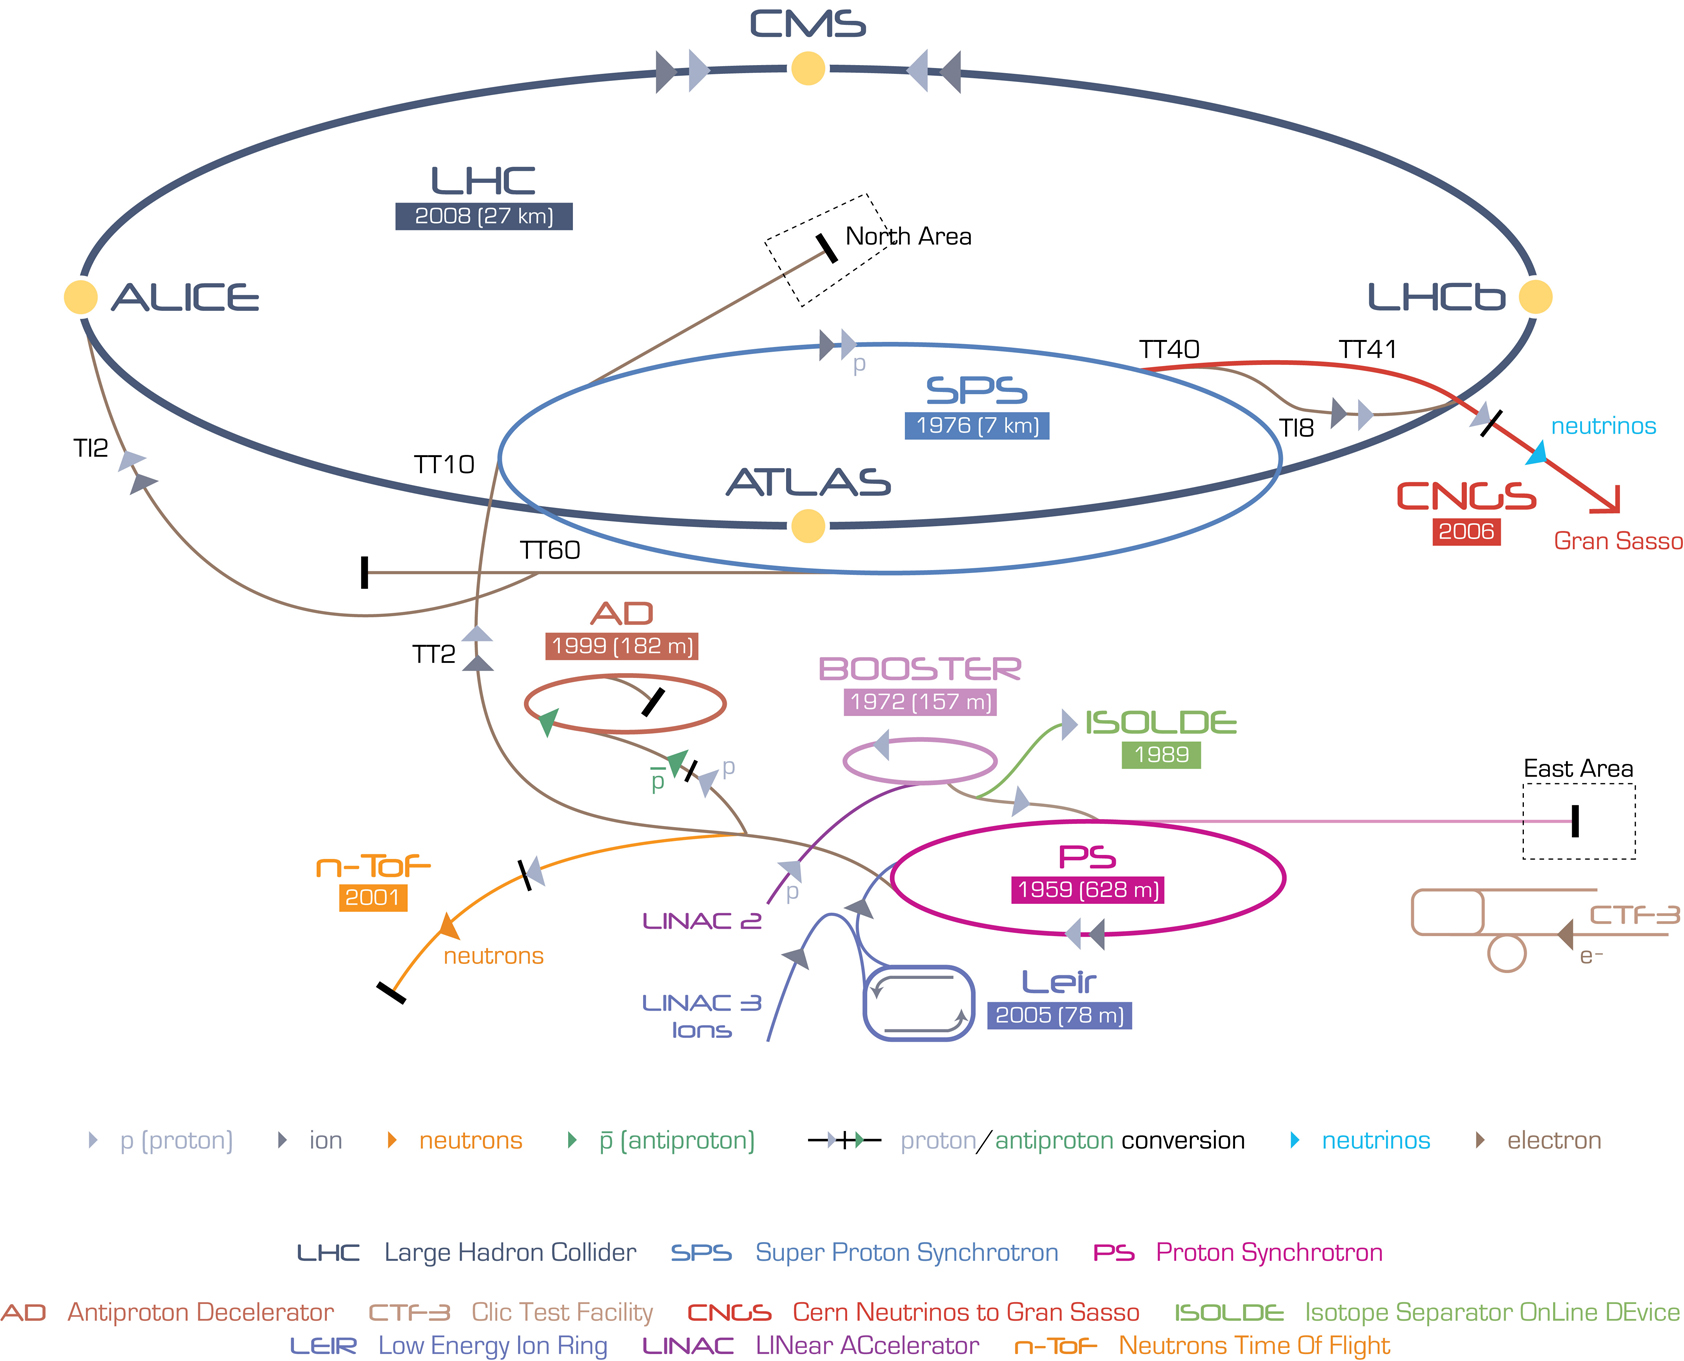
\includegraphics[width=1.\textwidth]{figures/setup/cern.jpg} %
	\caption{The accelerator complex at CERN. ATLAS can be seen inside the SPS on the LHC ring. Figure taken from Ref.~\cite{Christiane:1260465}}
	\label{fig:cern}%
\end{figure}

The LHC beams consist of bunches of protons or lead ions with a nominal bunch spacing of 25 ns that corresponds to 2808 bunches. 

In 2015, the LHC delivered an integrated luminosity of 0.49 \pb\ of \pbpb\ and 25 \pb\ of \pp\ data.


\section{The ATLAS Detector}
The ATLAS detector (Fig.~\ref{fig:atlas}) is a general purpose detector at the LHC. It uses a right-handed coordinate system with its origin at the nominal interaction point (IP) in the
 centre of the detector and the $z$-axis along the beam pipe. The $x$-axis points from the IP to the centre of the LHC ring, and the $y$ axis points upward. Cylindrical coordinates 
 $(r,\phi)$ are used in the transverse plane, $\phi$ being the azimuthal angle around the beam pipe. The pseudorapidity is defined in terms of the polar angle $\theta$ as 
 $\eta=-\ln\tan(\theta/2)$. The detector is symmetric in the forward-backward direction, with the positive $z$ direction being the $A$ side, and the negative $z$ direction being the $C$ side. It has full $2\pi$ coverage in azimuth.  The transverse momentum \pt, the transverse energy \Et, and the missing transverse energy \Etmiss\ are defined in the $x-y$ plane unless stated otherwise. The distance $\Delta R$ in the pseudorapidity-azimuthal angle space is defined as $\Delta R = \sqrt{\Delta \eta^2 + \Delta \phi^2}$.

The detector was designed keeping in mind the goals of the physics it aimed to explore, and as such has the following characteristics:
\begin{itemize}
\item Fast, radiation-hard electronics and sensor
\item Fine granularity to be able to manage large particle fluxes
\item Large acceptance in pseudorapidity and full azimuthal coverage
\item Good electromagnetic calorimetry for photon and electron identification
\item Good hadron calorimetry for accurate jet and missing transverse energy measurements
\item Good muon identification and momentum resolution
\item Highly efficient trigger system 
\end{itemize}

\begin{figure}[ht]
	\centering
	\includegraphics[width=0.7\textwidth]{figures/setup/atlas.pdf}
	\caption{The ATLAS detector. Figure taken from Ref.~\cite{Aad:2008zzm}.}	
	\label{fig:atlas}
\end{figure}


These design goals are achieved with the main subsystems: the inner detector, the calorimeter, the muon spectrometer, and the trigger system. The main analysis discussed in this thesis uses the inner detector, calorimeter, and the trigger system. The muon system is described for completeness.


\subsection{Inner Detector}
The inner detector (Fig.~\ref{fig:inner_det}) is designed to reconstruct the charged particle trajectories for particles with momenta down to 0.5 GeV in the interval $|\eta| < 2.5$. It is immersed in a 2T magnetic field from the central solenoid that covers a region of 5.3 m long and has a diameter of 2.5 m. The inner detector has capabilities for pattern recognition, momentum and vertex measurements, and electron identification. These measurements are made using the inner pixel detector, the semi-conductor tracker (SCT), and the transition radiation tracker (TRT). 

\subparagraph{Pixel system: } This system is segmented in \rphi and comprises of four pixel layers : the innermost insertable B layer (IBL) and three identical silicon pixel detectors. The IBL was added to the ATLAS detector during the first long shutdown of the LHC in 2013-2014. It consists of 14 carbon fiber staves, 2 cm wide and 64 cm long, surrounding the beam pipe at a mean radius of 33 mm, and covering a pseudorapidity region of $\pm 3$. Each stave consists of 26880 pixels in a matrix of 80 columns (50 $\mu$m pitch), by 336 rows (250 $\mu$m pitch) \cite{LaRosa:2016nbd, Capeans:1291633}. 
The other three layers layers have a pixel size in $\rphi \times z$ of $50 \times 400 \mu \mathrm{m}^2$. The accuracies in the barrel region are $10 \mu \mathrm{m}^2$ (\rphi) and $115 \mu \mathrm{m}^2 (z)$. The end cap regions have an accuracy of $10 \mu \mathrm{m}^2 (\rphi) $ and $115 \mu \mathrm{m}^2 (R)$. The hit resolution ranges from $\sim$ 8 (\rphi) and $\sim$ 40$\mu$m) ($z$) for the innermost layer, to $\sim$ 10 $\mu$m (\rphi) and $\sim$ 115$\mu$m ($z$) for the next three layers \cite{Aad:2008zzm}. The pixel detector has approximately 80.4 million readout channels. 

\subparagraph{Semi Conductor Tracker:} This subsystem has a coverage that overlaps with the pixel layers, and is arranged in concentric cylinders around the beam axis, with the end caps being disks perpendicular to the beam axis. The SCT has eight strip (80 $\mu$m pitch) layers that are crossed by each track. Small angle stereo strips (40 mrad) are used to measure both coordinates, with one set of strips in each layer, parallel to the beam direction. The end cap region has nine layers of double sided modules with strips in the radial direction, with each also having a mean pitch of 80 $\mu$m. The intrinsic resolution is $\sim$ 17$\mu$m (\rphi) and $\sim$ 580$\mu$m ($z$). There are approximately 6.3 million readout channels from the SCT.  \cite{Aad:2008zzm}.


\subparagraph{Transition Radiation Tracker:} The TRT uses a combination of a xenon based gas and 4mm diameter straw tubes and provides for a large number of hits (up to 36) per track. It covers the region $|\eta| <  2.0$, and has a resolution of $\sim$ 130$\mu$m in $r-\phi$, with no information in the $z$ direction. The barrel region of the TRT has straws that are 144 cm long and are parallel to the beam axis, with the wires divided into two halves at $\eta = 0$. The end-caps have 37 cm long straws in a radial configuration. The TRT has approximately 315,000 channels. \cite{Aad:2008zzm}.


\begin{figure}[ht]
	\centering
        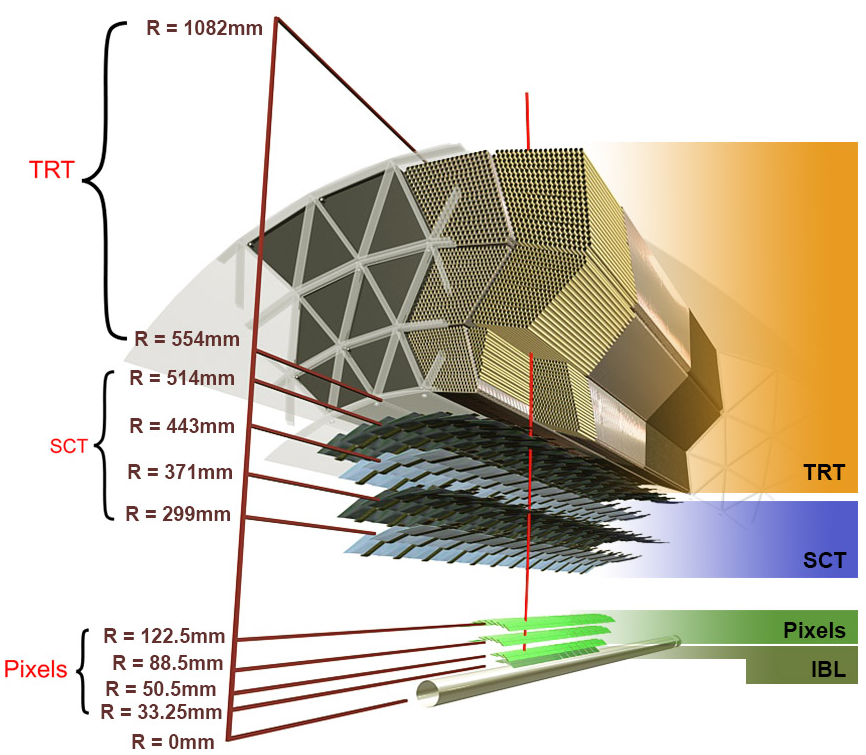
\includegraphics[width=0.7\textwidth]{figures/setup/inner_det.png}
          \caption{ATLAS Inner Detector System}
          \label{fig:inner_det}
\end{figure}

%%%%%%%%%%%%%%%%%%%%%%%%%%%%%%%%%%
\subsection{Calorimeter}
The calorimeter covers the eta range of < 4.9 for using a variety of different techniques. The parameters are summarized in the table below. Over the eta < 2.5, where there is overlap with the inner detector, the highly granular electromagnetic calorimeter is used for precision measurements of electrons and photons. The rest of calorimeter has coarser granularity that is sufficient for jet reconstruction. The calorimeter contains the electromagnetic and hadronic showers, and limits the punch through to the muon system. The EMCal has a radiation depth greater than 22 radiation lengths in the barrel, and greater than 24 radiation lengths in the end caps. The approximately 10 interaction lengths in the barrel and end cap provide good resolution for high energy jets. The total thickness of the calorimeter is 11 interaction lengths at $\eta = 0$. The calorimeter is divided into different subsystems, including the Liquid Argon Electromagnetic Calorimeter (LAr EMCal) and the Hadronic calorimeter (HCal).

\subparagraph{LAr EMCal: }
The EMCal covers the region $|\eta| < 1.475$ and has two end caps ($1.375 < |\eta| < 3.2$). It also contains the central solenoid. The barrel calorimeter is divided into two half barrels, separated by 4mm at $z = 0$. Each end cap is divided into two coaxial wheels, with the inner one covering $2.5 < |\eta| < 3.2$ and the outer one covering  $1.375 < |\eta| < 2.5$. The EMCal uses accordion shaped kapton electrodes and lead absorber plates that provide full azimuthal symmetry. The EMCal is subdivided into three sections in its depth over $|\eta| < 2.5$, the region used for precision physics. The $|\eta| < 1.8$ region also uses a pre-sampler detector that uses an active LAr layer to correct for energy lost upstream of the calorimeter. A main source of this loss is the central solenoid.

\subparagraph{Hadronic Calorimeter: }
The hadronic calorimeter consists of the tile, LAr Hadronic end cap, and the LAr forward calorimeter. The tile covers the region $|\eta| < 1.0$ , with its two barrels covering the range eta $0.8 < |\eta| < 1.7$. It uses steel as the absorber and scintillating tiles for the active material. The tile calorimeter extends radially from an inner radius of 2.28 m to 4.25 m. It has a three layer that are 1.5, 4.1, and 1.8 interaction lengths thick in the barrel region, and 1.5, 2.6, and 3.3 interaction lengths in the extended barrel region. The total detector thickness is 9.7 interaction lengths at $\eta = 0$. 

The LAr hadronic end cap calorimeter (HEC) consists of two independent wheels per end cap, and is behind the EMCal end cap. It extends out from $1.5 < |\eta| < 3.2$, and overlaps with the forward calorimeter and the tile calorimeter. The HEC covers the radial region of 0.475 to 2.03 m. 

The LAr Forward calorimeter provides coverage over the $3.1 < |\eta| < 4.9$. It is approximately 10 interaction lengths deep, and has three modules, one of which is optimized for electromagnetic measurements, while the other two for hadronic measurements. Each module is made of concentric rods and tubes parallel to the beam axis. 


A summary of the depth of the calorimeter in terms of the interaction lengths, as a function of pseudorapidity is shown in Fig.~\ref{fig:interaction_lenghts}.


\begin{figure}[ht]
	\centering
        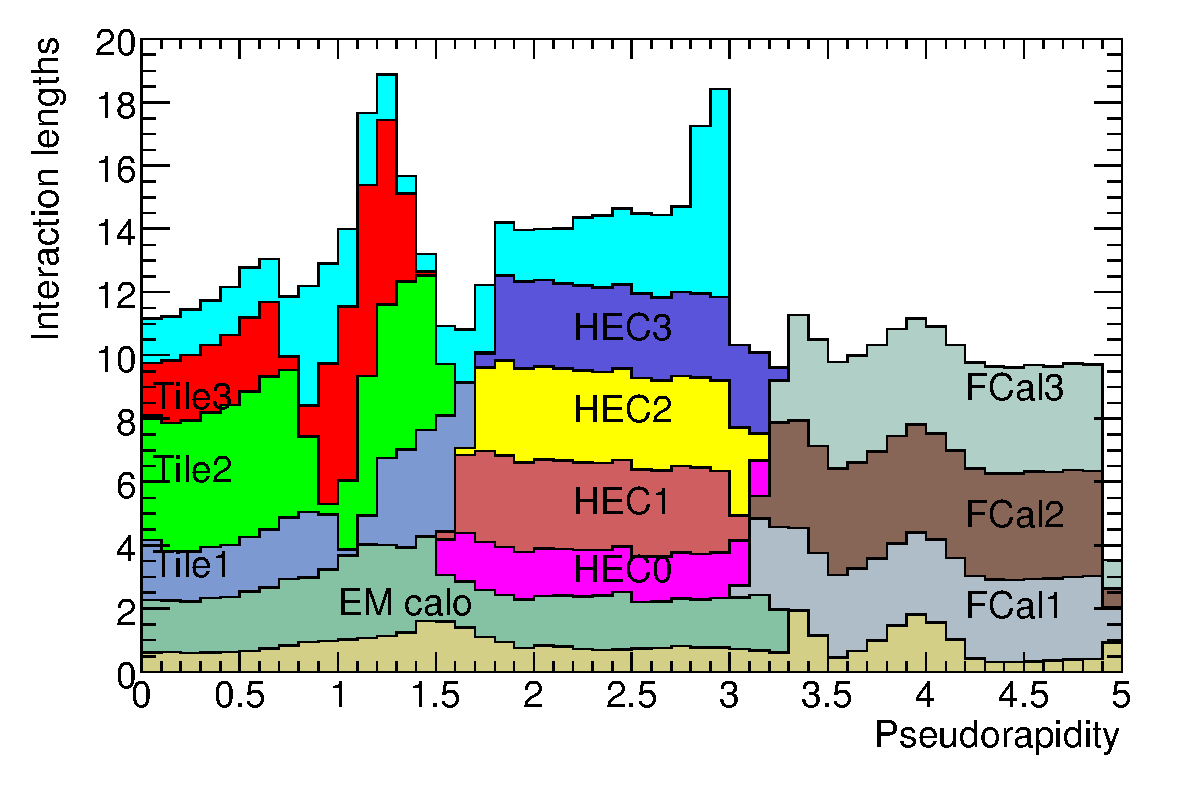
\includegraphics[width=0.7\textwidth]{figures/setup/interaction_lengths}
          \caption{Cumulative material in the calorimeter system in units of interaction length as a function of $|\eta|$.}
          \label{fig:interaction_lenghts}
\end{figure}

%%%%%%%%%%%%%%%%%%%%%%%%%%%%%%%%%%
\subsection{Muon Spectrometer}
The muon spectrometer is based on the magnetic deflection of muon tracks in the toroid magnets. The barrel toroid provides bending over the $|\eta| < 1.4$ range, and the end cap magnets provide bending in the $1.6 < |\eta < 2.7$ range. In the transition region ($1.4 < |\eta| < 1.6$), the magnetic deflection is from a combination of the barrel and end-cap fields. The barrel region has tracks that are measured in chambers in a cylindrical configuration around the beam axis. The transition and end-cap have chambers perpendicular to the beam axis. 


%%%%%%%%%%%%%%%%%%%%%%%%%%%%%%%%%%
\subsection{Other subsystems}
Other major subsystems of the ATLAS detector include the Zero Degree Calorimeter (ZDC), the trigger system

\subsubsection{ZDC}
The zero degree calorimeter plays a key role in determining the centrality of heavy ion collisions. It consists of quartz rods and tungsten plates, and measures neutral particles at $|\eta| >= 8.2$. It is made of four modules, one electromagnetic, and three hadronic. The Modules are made of 11 tungsten plates that are perpendicular to the beam direction. Photomultiplier tubes are used to detect the Cherenkov radiation from particle showers.


\subsubsection{Trigger System}
The trigger and data acquisition system (TDAQ) have different subsystems that are associated with sub-detectors. There are three distinct levels: L1, L2, and the event filter. The latter two form the High Level Trigger (HLT) system. The L1 trigger, shown in Fig.\ref{fig:L1_trigger}, uses custom electronics, while the HLT, shown in Fig.\ref{fig:HLT_trigger}, is software based. Each level uses information from the previous level to select events. 

The first level uses limited detector information and makes decisions based on muons, electron, photons, jets, and $\tau$-leptons carrying a high transverse momentum. It is also capable of identifying large missing and total transverse energy.  It has a maximum acceptance rate of 75kHz and makes a decision in less that 2.5$\mu$s. This event rate is further reduced to 200 Hz by the HLT that uses the full granularity and precision of the inner detector, calorimeter and muon systems to select events. 


\begin{figure}[ht]
	\centering
        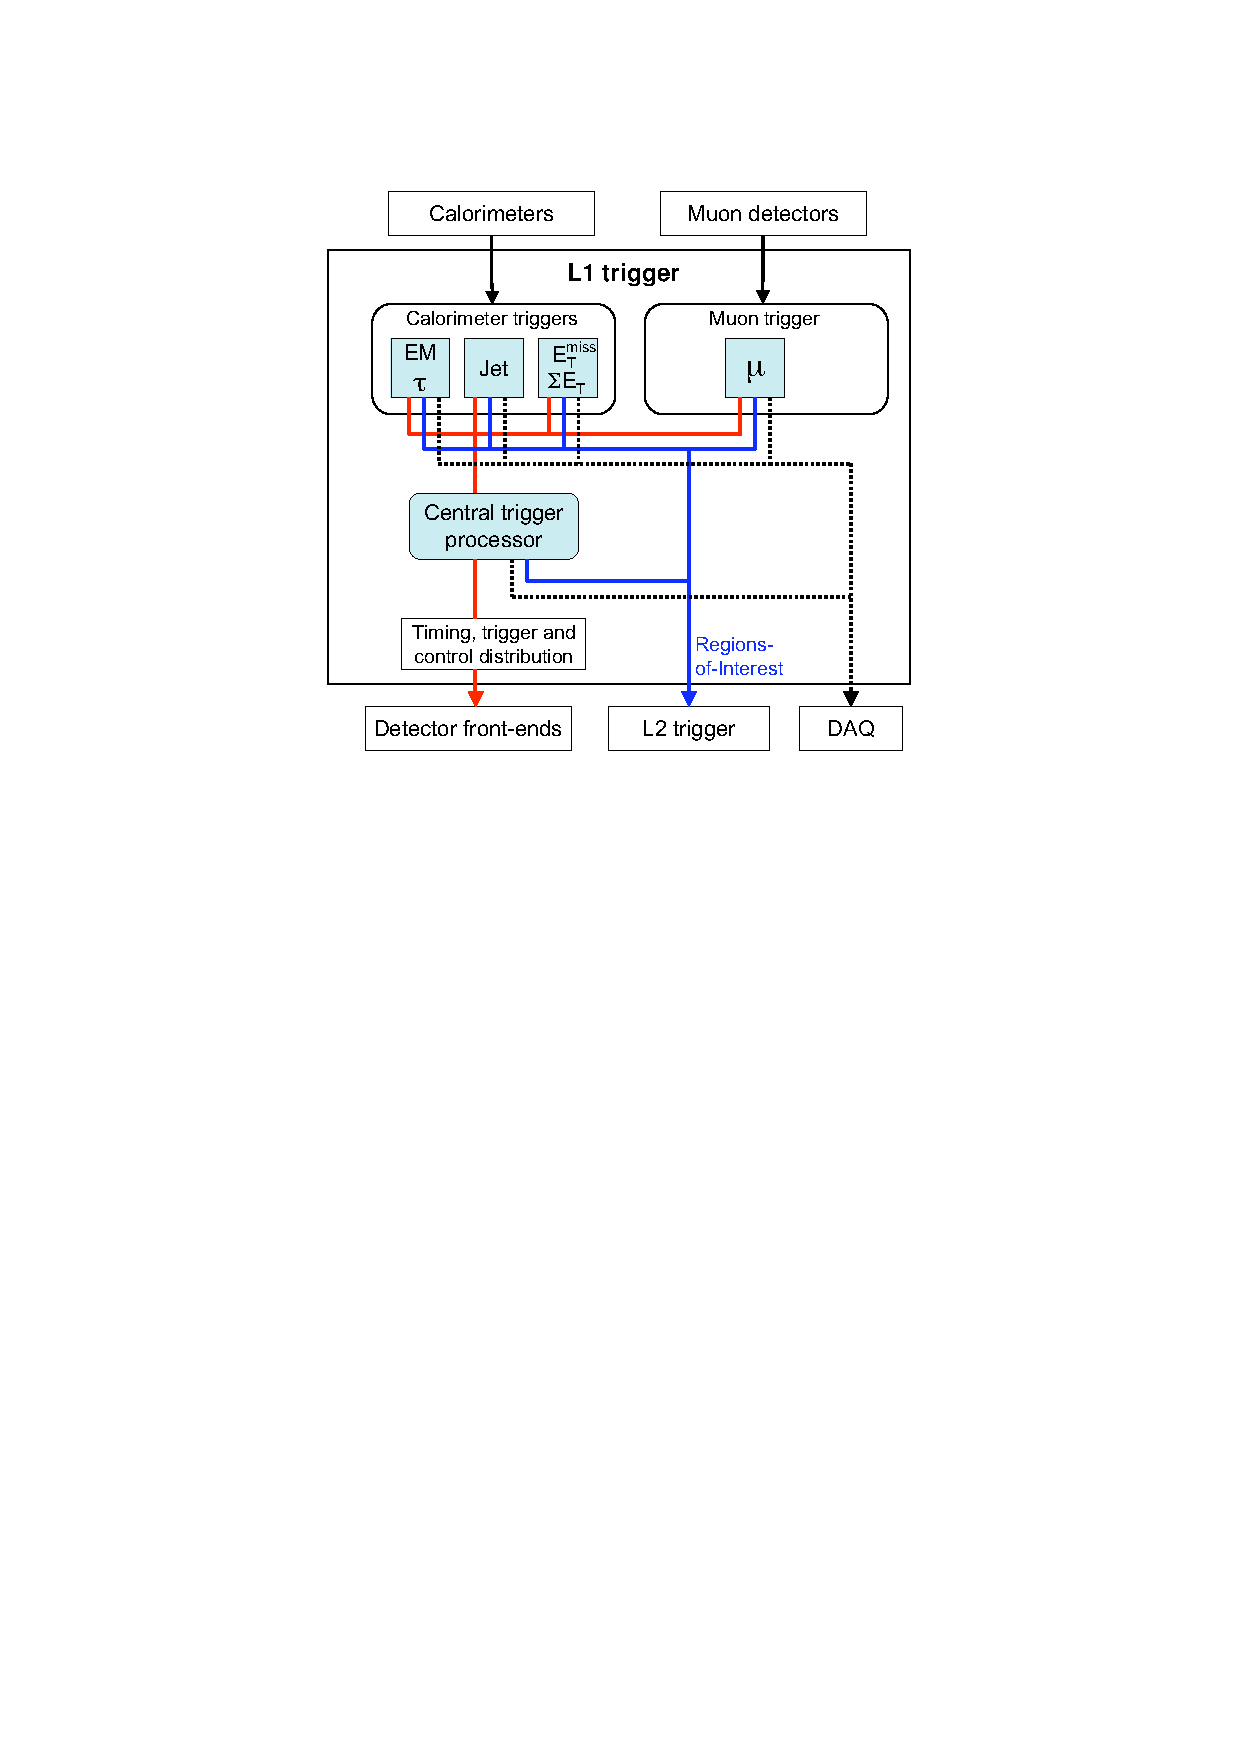
\includegraphics[width=0.7\textwidth]{figures/setup/L1_Trigger}
          \caption{Block diagram of the L1 Trigger System.}
          \label{fig:L1_trigger}
\end{figure}

\begin{figure}[ht]
	\centering
        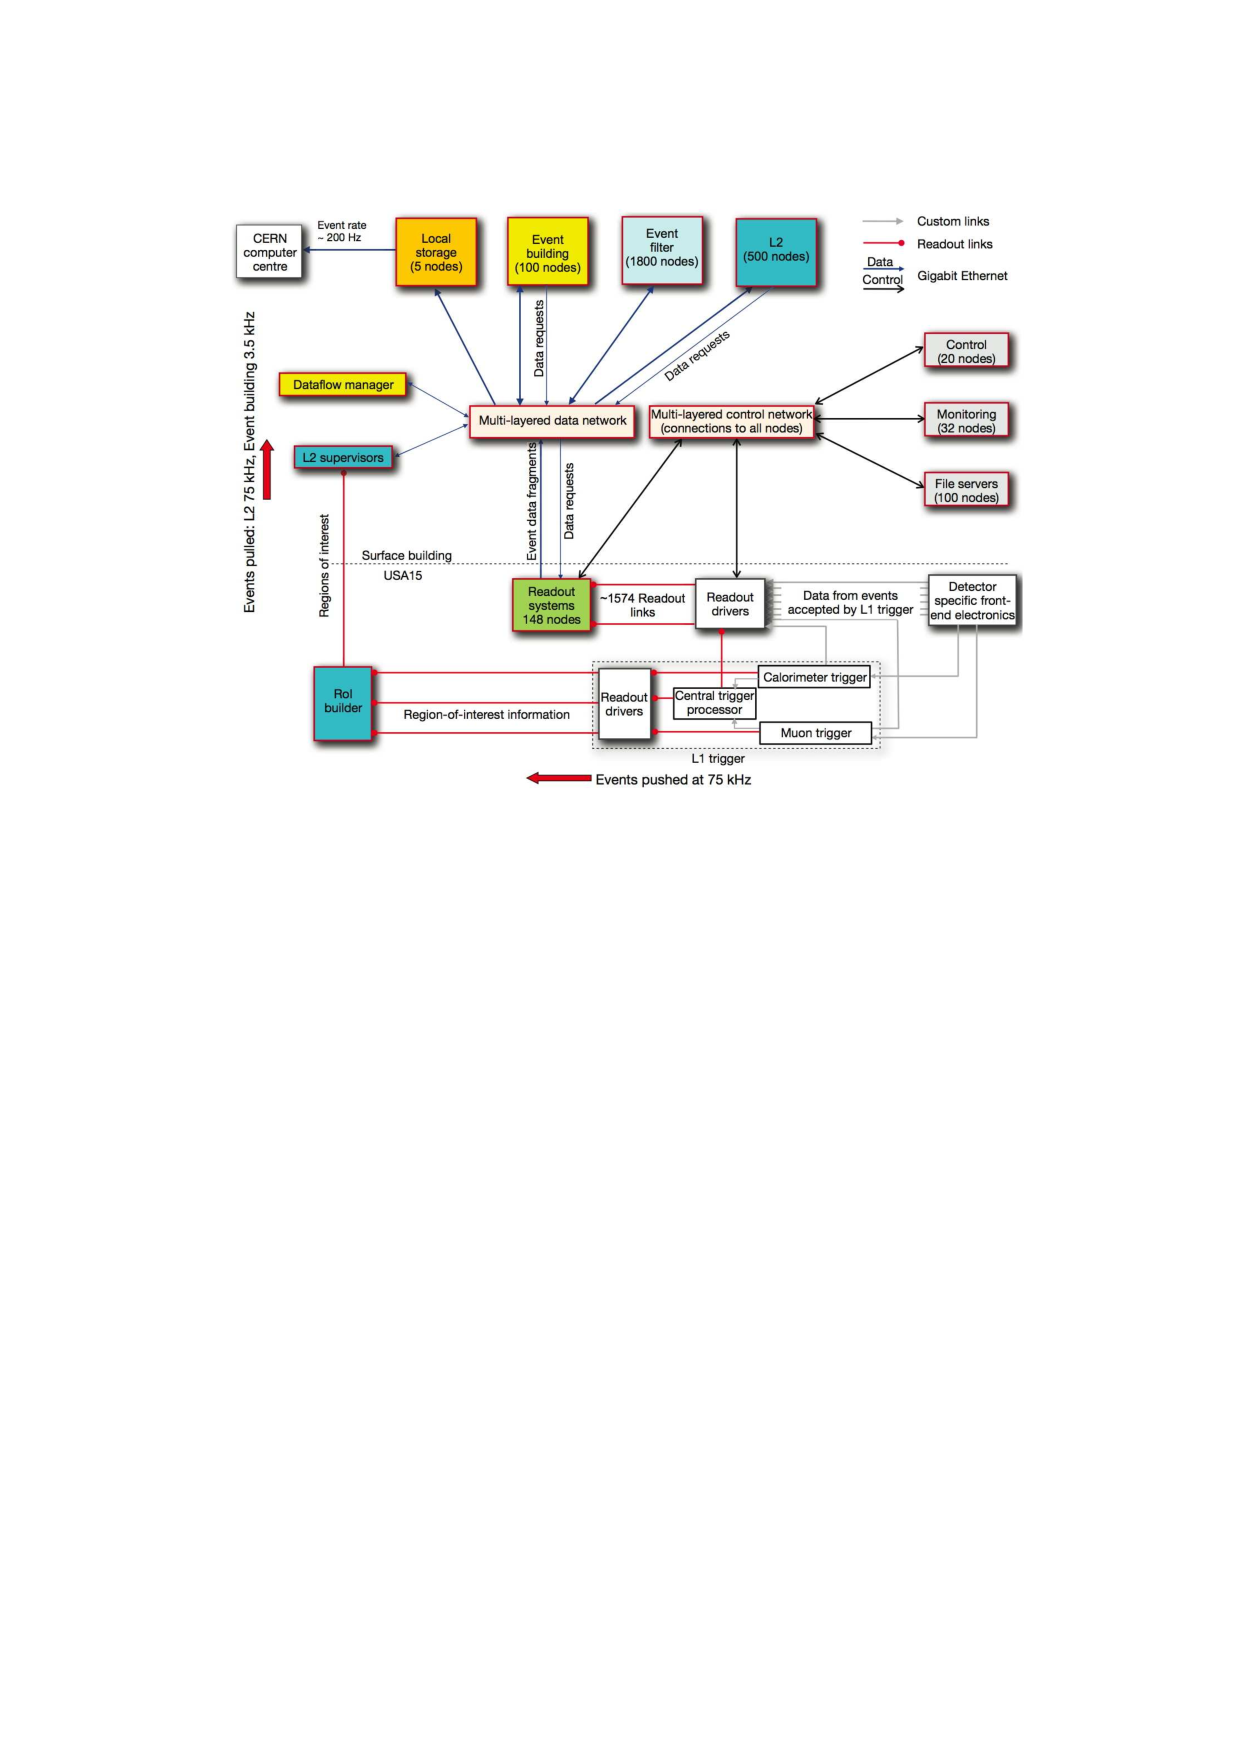
\includegraphics[width=0.7\textwidth]{figures/setup/HLT_Trigger}
          \caption{Block diagram of the HLT Trigger system.}
          \label{fig:HLT_trigger}
\end{figure}


%The $\eta$ coverage of the different detector systems can be seen in Fig.~\ref{fig:atlaspseudorap}.
%\begin{figure}[htbp!]
%	\centering
%	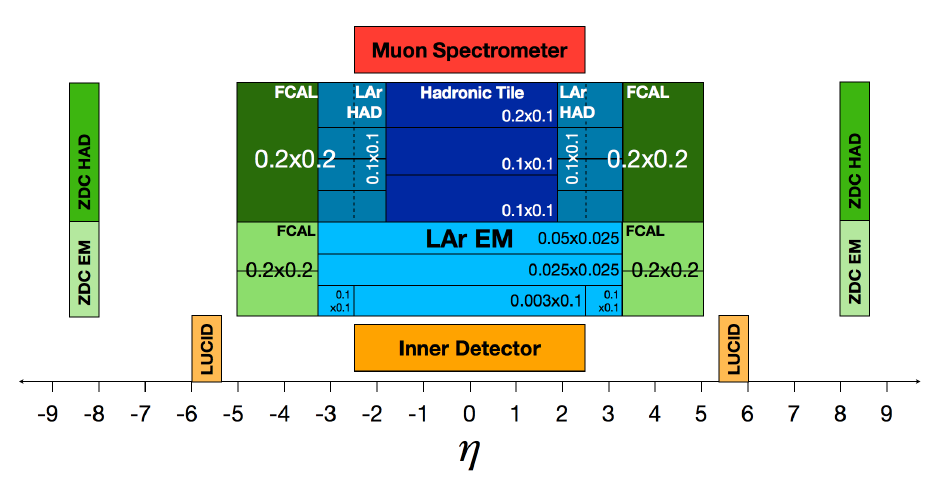
\includegraphics[width=0.7\textwidth]{figures/setup/atlaspseudorap.png} %
%	\caption{$\eta$ acceptance of the ATLAS detector.}	
%	\label{fig:atlaspseudorap}%
%\end{figure}

%%\begin{figure}[ht]
%%	\centering
%%	\includegraphics[width=0.7\textwidth]{figures/atlas.pdf} %
%%	\caption{The ATLAS detector. Figure taken from Ref.~\cite{Aad:2008zzm}.}	
%%	\label{fig:atlas}%
%%\end{figure}





%
%\subsection{Magnet System}
%The ATLAS detector has a magnet configuration that consists of a thin superconducting solenoid surrounding the inner detector cavity, and three large superconducting toroids arranged symmetrically around the calorimeters. The inner detector is immersed in a 2 T magnetic field, and achieves pattern recognition, momentum and vertex measurements, and electron identification by a combination of high resolution semiconductor pixel and strip detectors in the inner tracking volume, and a straw tube detector for transition radiation in the outer volume. 



%\FloatBarrier

%%%%%%%%%%%%%%%%%%%%%%%%%%%%%


%\chapter{Theoretical Introduction}
%\label{sec:intro}
%% !TEX encoding = UTF-8 Unicode
% !TEX root = thesis-ex.tex

\section{Quantum Chromo-Dynamics}

Quantum Chromo-Dynamics (QCD) is a relativistic non-abelian gauge theory, with symmetry group SU(3), which describes the strong interaction between quarks and gluons. Quarks are charged subatomic particles that are the fundamental constituents of matter and gluons are gauge bosons that are mediators of the strong interaction between quarks. In its form, QCD appears similar to QED~\cite{Seymour:2005hs}, however, since the gluons of the strong force carry color charge, solutions to the QCD Lagrangian become more complicated. The QCD Lagrangian~\cite{qcdbook} is 

\begin{equation}
\mathcal{L}=\bar{\psi}_{i}(i\gamma^{\mu}\partial_{\mu}-m_{i})\psi_{i}-g\bar{\psi}_{i}\gamma^{\mu}t_{ij}^{a}\mathcal{A}_{\mu}^{a}\psi_{j}-\frac{1}{4}F^{\mu\nu}_{a}F_{\mu\nu}^{a},
\label{eq:lagrangian}
\end{equation}

where $\psi$ is the spin-1/2 quark field (quark), $m_{i}$ is the quark mass,  $\mathcal{A}_{\alpha}^{A}$ is the spin-1 gluon field (gluon), $t_{ij}^{a}$ is a generator from the fundamental representation of the $SU(3)$ group which describes the interactions between quark and gluon fields. The field strength tensor $F^{\mu\nu}_{a}$ is derived from $\mathcal{A}_{\alpha}^{A}$,

\begin{equation}
F_{\mu\nu}^{a}=\Big[ \partial_{\mu}\mathcal{A}_{\nu}^{a} - \partial_{\nu}\mathcal{A}_{\mu}^{a} - g f^{abc}\mathcal{A}_{\mu}^{b}\mathcal{A}_{\nu}^{c}\Big]
\label{eq:fieldtensor}
\end{equation}

where the indices $a$, $b$, and $c$ sum over the eight color degrees of freedom of the gluon field and $f^{abc}$ are the structure constants of the $SU(3)$ color group. The term $g=\sqrt{4 \pi \alphaS }$ is related to the strong force coupling constant \alphaS.

\begin{figure}
	\centerline{
		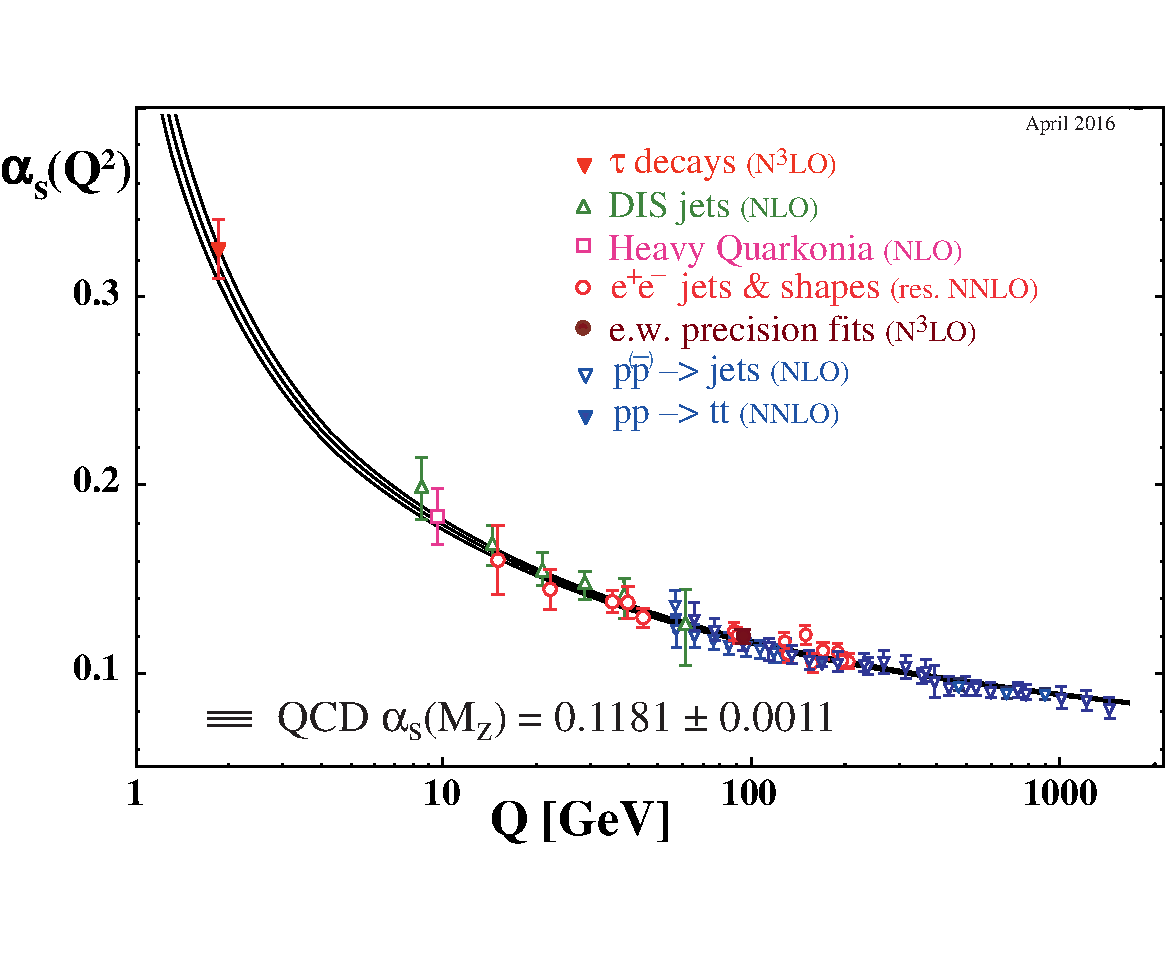
\includegraphics[width=0.6\textwidth]{figures/asq-2015.pdf} 
	}
	\caption{Strong force coupling constant \alphaqs, which decreases with increasing four-momentum transfer $Q=\sqrt{|q^{2}|}$.  Figure taken from Ref.~\cite{pdg:2018}.}
	\label{fig:strongforceconstant}
\end{figure}

In~\ref{eq:lagrangian}, the left-most term, $\bar{\psi}_{i}(i\gamma^{\mu}\partial_{\mu}-m_{i})\psi_{i}$, is the Dirac equation describing a free particle. To account for interactions with the field, additional terms are present. The middle term, $g\bar{\psi}_{i}\gamma^{\mu}t_{ij}^{a}\mathcal{A}_{\mu}^{a}\psi_{j}$, describes the coupling between quarks and gluons, and the last part of the Lagrangian, $\frac{1}{4}F^{\mu\nu}_{a}F_{\mu\nu}^{a}$, is the kinetic term from the gluon field. 

The third term, $f^{abc}\mathcal{A}_{\mu}^{b}\mathcal{A}_{\nu}^{c}$, in the field strength tensor $F^{\mu\nu}_{a}$, is the non-abelian term that distinguishes QCD from QED. This gives raise to three- and four-point gluon vertices, resulting in the three basic vertices of QCD, shown in Figure~\ref{fig:qcdvertices}. 

\begin{figure}
	\centerline{
		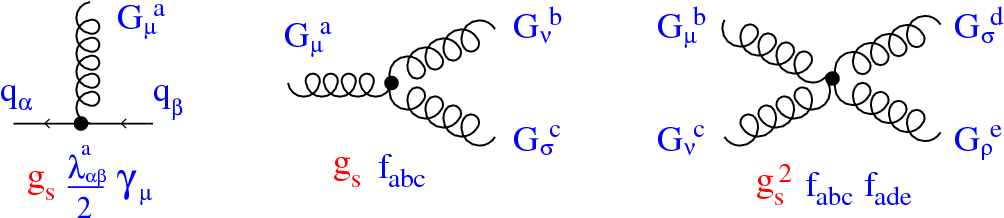
\includegraphics[width=0.9\textwidth]{figures/qcd_vertices.pdf} 
	}
	\caption{Three types of QCD vertices: the basic quark-gluon QCD vertex (left), three-gluon self interaction (center), and four-gluon self interaction (right). }
	\label{fig:qcdvertices}
\end{figure}

A consequence of gluon self interactions in QCD is the fundamental property of asymptotic freedom: the fact that the strong force coupling constant \alphaqs\ decreases with increasing energy scales, or by the uncertainty principle, smaller distances. The four-momentum transfer $Q=\sqrt{|q^{2}|}$, where $q$ is the four momentum of a virtual particle responsible for an interaction, determines the energy and distance scales ($d\sim 1/Q$) probed. Asymptotic freedom also explains the interpretation that quarks and gluons are point-like particles since the distances probed inside the proton can be arbitrarily small. The behavior of \alphaS\ at larger distances, or smaller energies shows a rapid increase in the coupling between quarks and gluons. A direct consequence of this is that particles which interact via the strong force are highly confined: they cannot exist freely at macroscopic distances. Only color singlet states - quark-antiquark pairs (mesons) and three quark states (baryons) exist stably~\cite{Seymour:2005hs}.  The behavior of \alphaS\ is shown from various measurements as a function of four-momentum transfer $Q$ in Fig.~\ref{fig:strongforceconstant}. 

There have been several techniques developed for performing QCD calculations. The two established methods are perturbative QCD (pQCD)~\cite{Brock:1993sz} and lattice QCD~\cite{creutz1985quarks}. Lattice QCD is used predominantly for calculations at lower energies where \qsquare\ is small and \alphaS\ is large. These calculations are performed below the characteristic QCD scale $\lambda_{QCD}\sim200$ MeV, where $\alphaS\sim 1$. Lattice QCD calculations have been successful in describing experimental data on the properties of nucleons, such as their mass mass~\cite{Borsanyi:2014jba}. Additionally, these computationally intensive calculations support experimental evidence of a new state of matter that exists at high temperatures and densities called the Quark Gluon Plasma (QGP)~\cite{Harris:1996zx,Adcox:2004mh,Adams:2005dq,Arsene:2004fa,Back:2004je}. If the \qsquare\ of a system is above $\lambda_{QCD}$, meaning \alphaS\ is sufficiently small, pQCD calculations can be used because an order-by-order expansion of the Lagrangian in powers of \alphaS\ is appropriate. In this high \qsquare\ regime, individual quarks or gluons in the nucleus can be resolved. Whereas, in the low \qsquare\ regime, where lattice QCD calculations are used, only individual nucleons and not their constituents can be observed. The measurement presented in this dissertation will rely on tools that were developed to work at energy scales where pQCD calculations can be used.

\begin{figure}[hb]
	\centerline{
		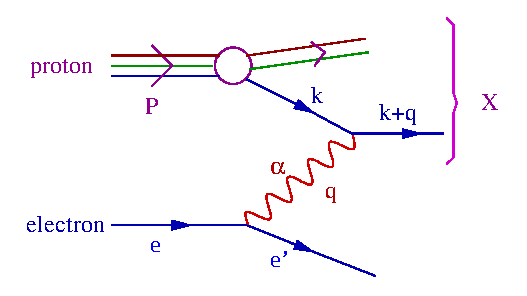
\includegraphics[width=0.65\textwidth]{figures/dis_2.pdf} 
	}
	\caption{ The DIS process that takes place in $e^{\pm}p$ collisions with an exchange via a virtual photon $\gamma^{*}$. Figure taken from Ref.~\cite{Iancu:2012xa}. }
	\label{fig:dis}
\end{figure}


\section{Deep Inelastic Scattering}

The proton, the fundamental building block of nuclear matter in nature, is a fermion with one positive unit of electric charge, a spin of $1/2 \hbar$. However, much more has been discovered about its fundamental properties and constituents in recent years. Almost half a decade ago the so called $naive\ parton\ model$~\cite{Bjorken:1969ja,Peskin:1995ev} of the proton was proposed: the proton was made out of non-interacting point-like constituents called partons, which were thought to be charged fermions, possibly bound together by some other neutral particles. This model was first supported by evidence from through lepton-nucleon Deep Inelastic Scattering (DIS) experiments from the SLAC-MIT collaboration~\cite{Whitlow:1990gk}. Commonly, this was done with an electron and a proton, with incoming four-momenta $e$ and $P$, respectively, and a virtual photon with four-momentum $q$ acting as the exchange particle. This process, $ep \rightarrow eX$, where $X$ are the remnants of the proton, is shown in Fig.~\ref{fig:dis}. From these quantities, we define two important variables in DIS, the first is the proton longitudinal momentum fraction carried by its constituent parton, $Bjorken$-\xb:

\begin{equation}
\xb = \frac{\qsquare}{2P\cdot q} = \frac{\qsquare}{2M\nu},
\label{eqn:xb}
\end{equation}

where $\nu$ is the energy of the virtual photon in the proton rest frame. The second variable is the lepton momentum fraction transferred to the proton:

\begin{equation}
y = \frac{P\cdot q}{P \cdot e} = \frac{\nu}{E},
\label{eqn:ydis}
\end{equation}

where $E$ is the energy of the lepton in the proton rest frame. The resolving power of the photon goes as $R^{2} \sim 1/\qsquare$, meaning that for the proton, with a proton radius of $R_{p}\sim8$ fm, if $\qsquare \equiv -q^{2} \ll 1\ \mathrm{(GeV/c)^2}$, the photon will interact elastically with the proton nucleus as a whole. If $\qsquare \equiv -q^{2} \gg 1\ \mathrm{(GeV/c)^2}$, the photon will interact inelastically with the proton, and will probe its individual constituents, partons. This inelastic scattering regime, where energy is transferred from the photon to the proton,   $\qsquare \gg 1/R_{p}^{2} \sim 1 \mathrm{(GeV/c)^2}$ corresponds to $\qsquare \gg m_{p}^{2}$, where $m_{p} \sim 1 \mathrm{(GeV/c)^2}$ is the proton mass. This puts a minimum requirement on \qsquare\ to effectively disassemble the proton and is the region of phase-space where DIS occurs. This is usually named as the boundary to the inelastic scattering regime. However, to avoid the creation of purely resonant states, a second criteria is often the energy of the hadronic final state. Thus, in some QCD global analysis, $\qsquare>4$ GeV is chosen as the boundary.

The sub-structure of hadrons in DIS can be parameterized by so called structure functions $F_{1}(x,\qsquare)$ and $\ftwo(x,\qsquare)$~\cite{Kovchegov:2012mbw}, which are distribution functions describing the structure of a baryon. Using a linear combination of the two structure functions

\begin{equation}
F_{L}(x,\qsquare) = \ftwo(x,\qsquare) - 2xF_{1}(x,\qsquare),
\end{equation}

the DIS cross section can be parameterized as  

\begin{eqnarray}
\frac{d^{2}\sigma}{dx\ d\qsquare} = \frac{2\pi\alphaS^{2}}{xQ^{4}}\big[(1 + (1-y)^{2})\ftwo(x,\qsquare) - y^{2}F_{L}(x,\qsquare)\big].
\label{eqn:discrosssection}
\end{eqnarray}
	
	
As introduced above $y$ is the fractional energy loss of the lepton and is usually small in most of the kinematic plane. The majority of experiments impose a cut of $y < 0.8$ to keep QED radiative corrections small. As a result, $F_{L}$ can be neglected leaving only the  contribution from \ftwo. In fact, the structure function $F_{L}$ is only measured where \qsquare\ is close the so called kinamtic limit~\cite{Seymour:2005hs}, which is $\qsquare < (p + l)^2$. 


\section{Parton Distribution Functions}


\begin{figure}
	\centerline{
		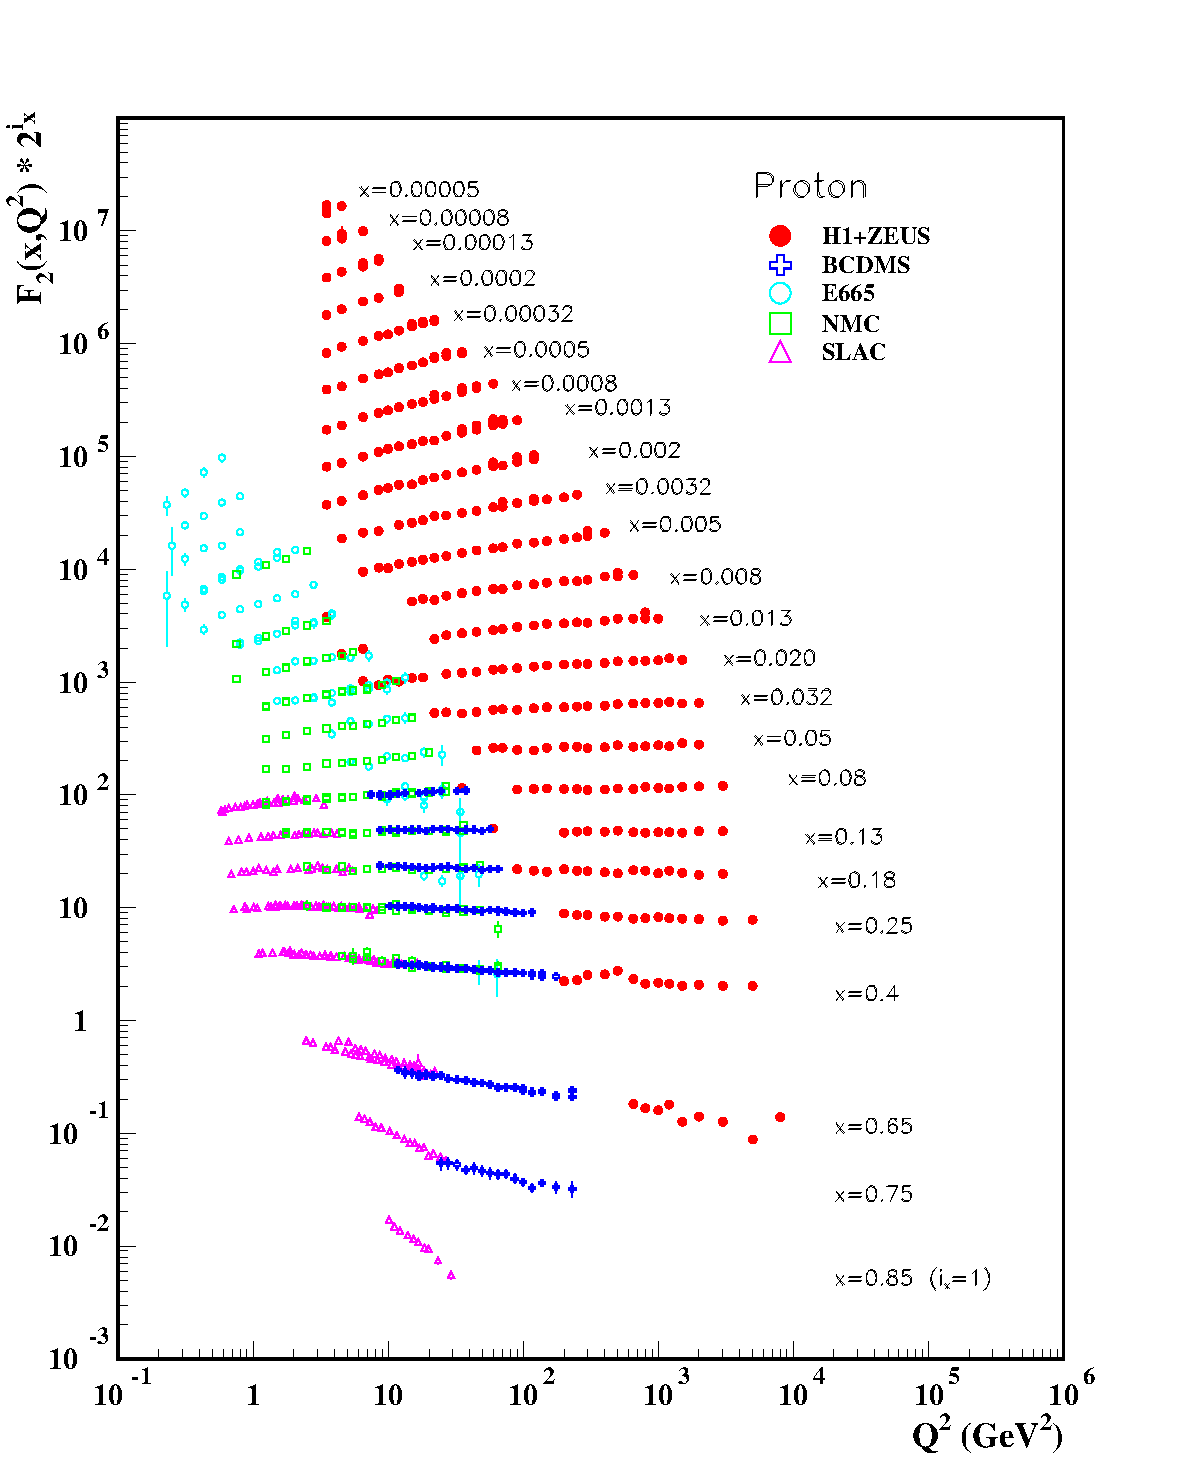
\includegraphics[width=0.65\textwidth]{figures/f2collider_logf2.pdf} 
	}
	\caption{ Summary of \ftwo\ structure function data plotted as a function of \qsquare\ for different values of \xb. Figure taken from Ref.~\cite{pdg:2018} }
	\label{fig:f2}
\end{figure}



The DIS interaction through a photon, which does not couple to gluons, first assumed that the \ftwo\ structure function purely described quark distributions. In the naive parton model, the point-like nature of the proton constituents implied there is no cutoff on the distances that can be probed, meaning there should not be a dependence on \qsquare. This meant that the \ftwo\ structure function can be rewritten with no \qsquare\ dependence purely as the sum over flavors of quark and antiquark parton distribution functions (PDFs) $q_{i}(x)$ and $\bar{q}_{i}(x)$

\begin{equation}
F_{2}(x,\qsquare) \sim F_{2}(x) = \sum_{i}^{}e_{i}\big(xq_{i}(x) + x\bar{q}_{i}(x)\big),
\end{equation}

where $e_{i}$ is their respective charge. The PDFs are probability density functions representing the probability of finding a quark with flavor $i$ having a longitudinal momentum fraction $x$ and $x+dx$. Therefore, $xq_{i}(x)$ is the number of quarks with flavor $i$ that have a longitudinal momentum fraction $x$ between $x$ and $x+dx$. The results of \ftwo\ structure function data are shown in Fig.~\ref{fig:f2}~\cite{Abramowicz:2014jak, Pasechnik:2016wkt, Adams:1996gu, Evans:2008zzb,Whitlow:1991uw}, where a lack of \qsquare\ dependence, called Bjorken scaling~\cite{Bjorken:1968dy}, is seen for $x>0.1$. However, experiments that probed lower \xb\ saw a non-linearity, or a scaling violation, of \ftwo\ with changing \qsquare.

\begin{figure}
	\centerline{
		\includegraphics[width=0.75\textwidth]{figures/proton.pdf} 
	}
	\caption{A simple picture of the proton, with three quarks connected by three gluons (left). At shorter timescales, quantum fluctuations exist and the proton picture becomes more complex (right).  }
	\label{fig:proton}
\end{figure}

The linearity of the \ftwo\ structure function was proposed based on the assumption that protons constituents are non-interacting. This ignores QCD radiative processes, the process in which quarks interact with and radiate gluons. Probing the proton at low energies, the picture is one of three partons - two up quarks and a down quark as shown on the left of Fig.~\ref{fig:proton}. These so called valence quarks are strongly interacting and are held together by gluons. However, at smaller distances and shorter timescales, the picture of the proton becomes more complicated, as seen on the right of Fig.~\ref{fig:proton}. In this regime, gluons can be seen splitting into short lived quark-antiquark pairs (sea quarks), or into gluon-gluon pairs. Additionally, it was found that the total momentum contribution of all quarks inside the proton, when the quark PDFs are integrated over a wide range of x, was roughly 50\%~\cite{qcdbook}. All this information strongly suggested the possibility that gluons carry a significant momentum fraction of the proton, depending on the \xb\ and \qsquare\ of the interaction. The inclusion of gluons into the nucleus wavefunction is what gave rise to the scaling violation seen in the various experiments at lower-\xb. As a result, the PDFs for quarks and gluons have to be expressed as a function of \xb\ and \qsquare: $q_{i}(x,Q^{2})$ for quarks and $g_{i}(x,Q^{2})$ for gluons. This new picture of the proton is is sometimes called the $improved\ parton\ model$ or just the parton model, for brevity.

\begin{figure}
	\centering
	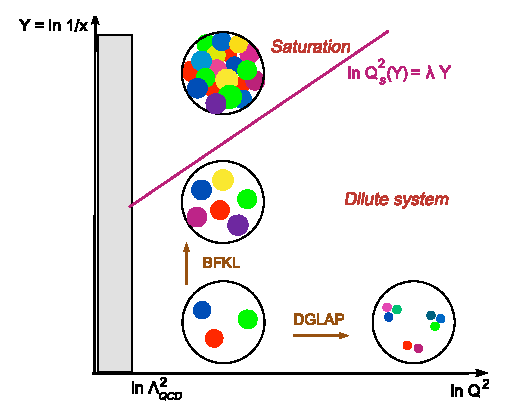
\includegraphics[width=0.45\textwidth]{figures/dglap_bfkl.pdf} 
	\caption{ Schematic showing the BFLK evolution in $ln(1/\xb)$ and DGLAP evolution in $ln(\qsquare)$ (left figure). The saturation scale $Q_{S}$ is represented by the diagonal line.}	
	\label{fig:cgc}
\end{figure}

In the regime where pQCD can be used ($\alphaS > \lambda_{QCD}$), techniques have been developed to describe the evolution of PDFs both with \xb\ and \qsquare. The Dokshitzer-Gribov-Lipatov-Altarelli-Parisi (DGLAP) equations~\cite{Gribov:1972rt,Gribov:1972ri,Dokshitzer:1977sg,Altarelli:1977zs} describe the evolution of PDFs at as a function of $ln(\qsquare)$, at a fixed \xb. The other set of equations, describing the PDF dependence on $ln(1/\xb)$ at fixed \qsquare, are the Balitsky-Fadin-Kuraev-Lipatov (BFKL) evolution equations~\cite{Balitsky:1978ic, Kuraev:1977fs, Fadin:1975cb, Lipatov:1976zz}. These sets of equations describing the evolution of parton densities in \qsquare\ and $x$ are considered to be the most fundamental equations in pQCD. The BFLK equation will be of particular interest to this thesis because of its role in evolving PDFs to low-\xb. A schematic representation of the BFLK and DGLAP evolutions in the $ln(1/x)$ vs $ln(\qsquare)$ phase-space is shown in~\ref{fig:cgc}.

\begin{figure}
	\centering
	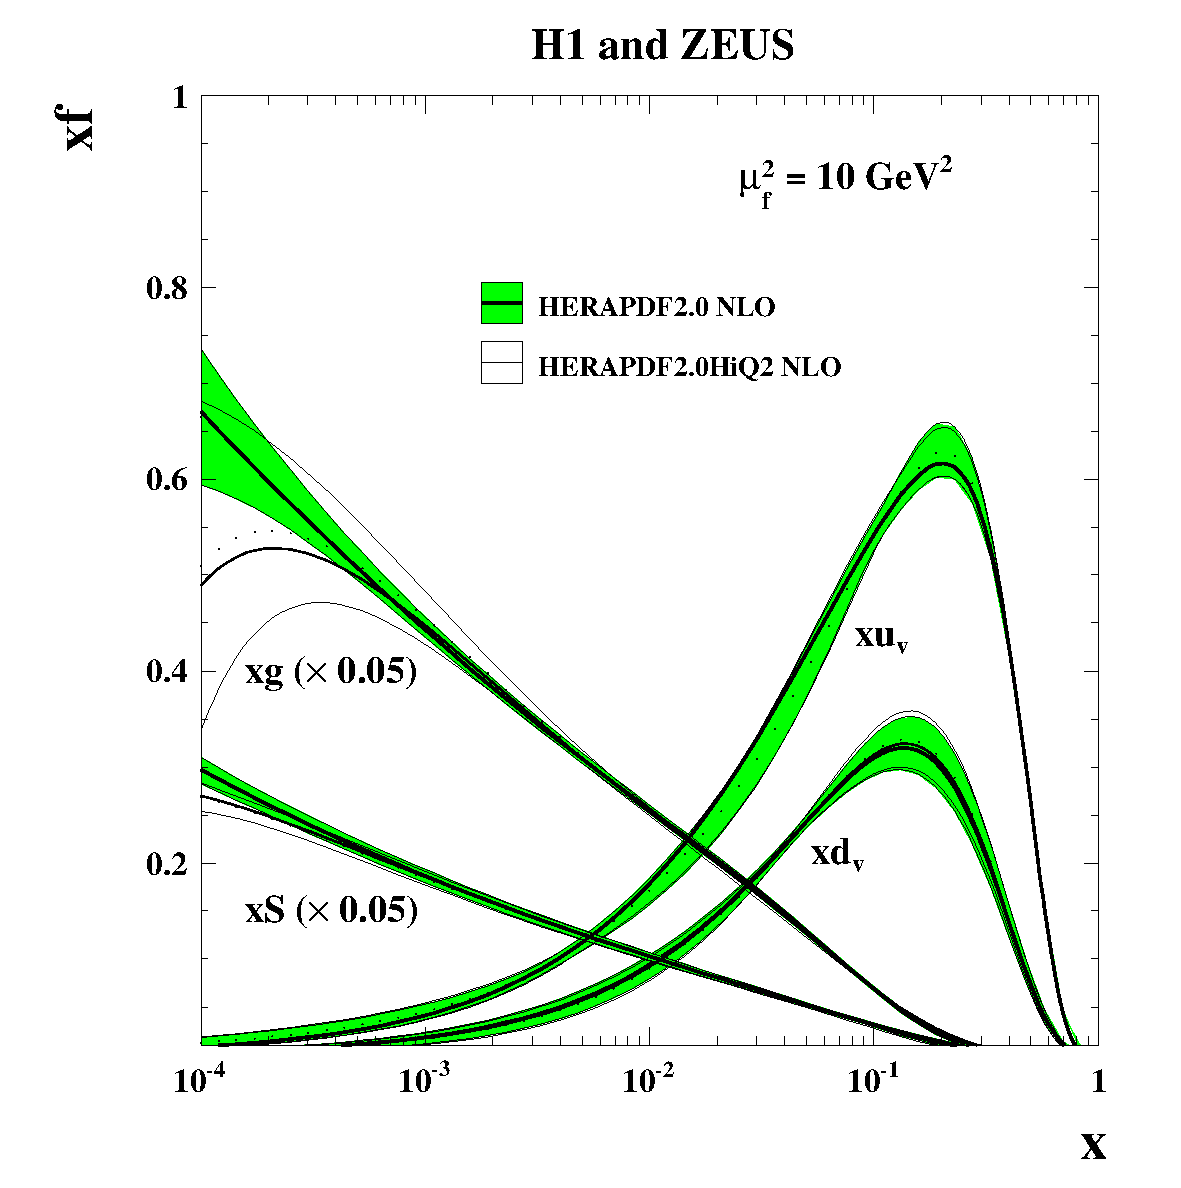
\includegraphics[width=0.48\textwidth]{figures/d15-039f54a.pdf} 
	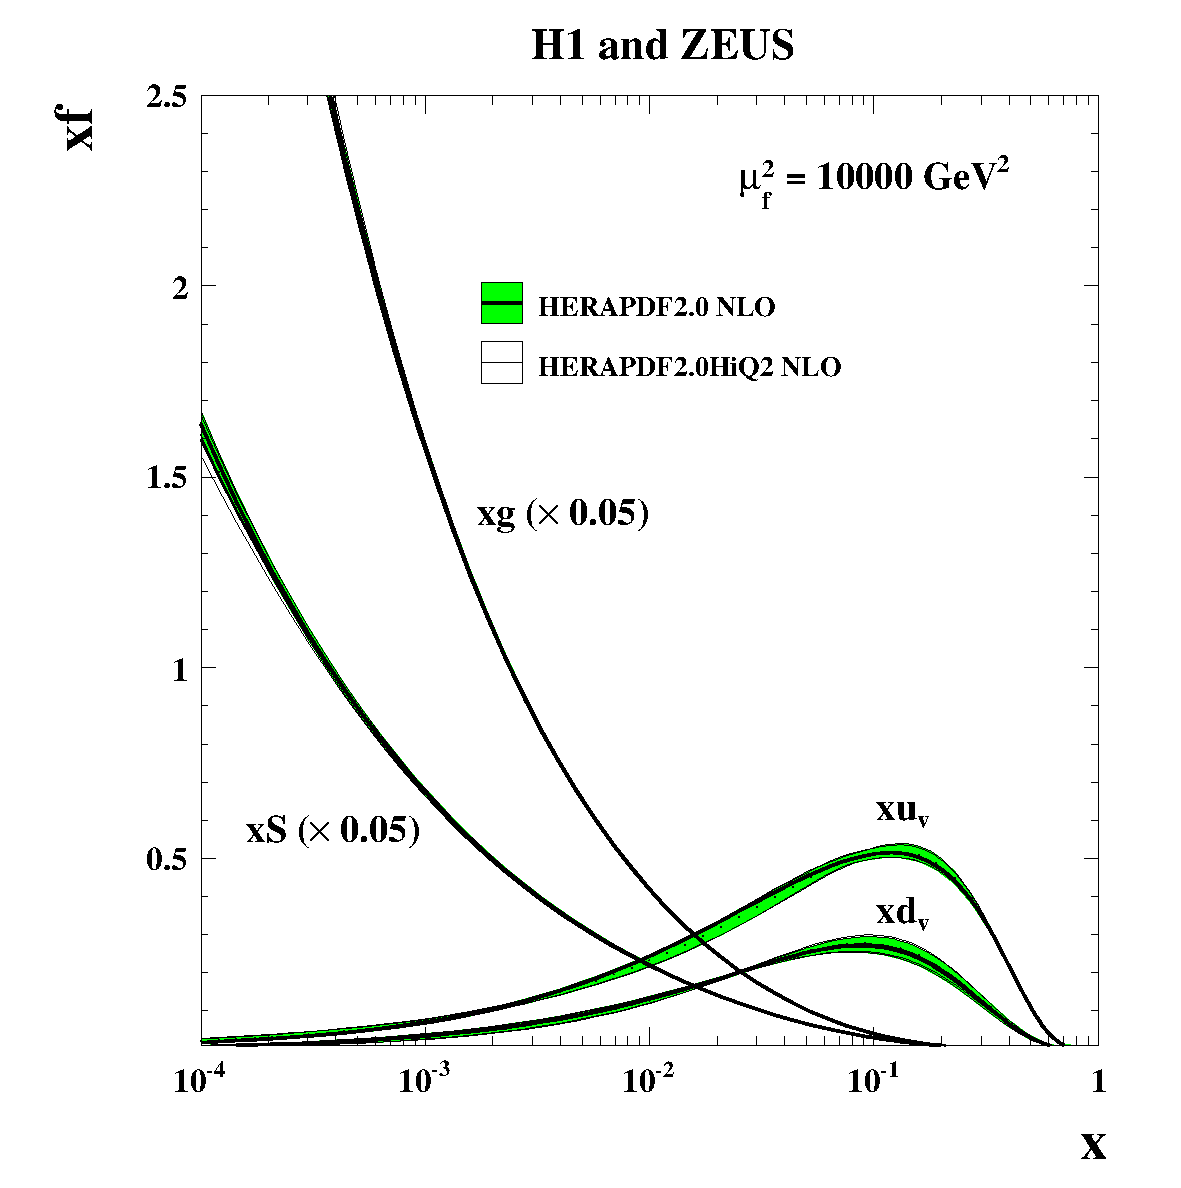
\includegraphics[width=0.48\textwidth]{figures/d15-039f55a.pdf} 
	\caption{PDFs obtained at different $Q^{2}$ by the H1 and ZEUS collaborations. The gluon PDFs are scaled so they would fit on the plots with the quark PDFs. Note that the observable plotted is $xq_{i}(x,\qsquare)$. Figure taken from Ref.~\cite{Abramowicz:2015mha}.}	
	\label{fig:pdfsintro}
\end{figure}

Over time, global QCD analysis of structure functions in deep inelastic lepton-nucleon scattering at HERA, as well as jet and hadron cross sections at the LHC, Tevatron, and RHIC were performed in a wide kinematic range, providing several new sets of PDFs with the highest degree of precision reached so far~\cite{Dulat:2015mca,Ball:2017nwa,Harland-Lang:2014zoa,Abramowicz:2015mha}. Examples of quark and gluon PDFs from DIS experiments at different $Q^{2}$ from the H1 and ZEUS collaborations are shown in Fig.~\ref{fig:pdfsintro}. These global QCD analyses show that the \gx\ found to rise rapidly at small \xb\ in the proton. The rapidly increasing \gx\ at $\xb \ll 1$ is explained by gluon radiation (bremsstrahlung) of soft gluons, where a parton with high-\xb\ collinearly emits a gluon with an $\xb_{1} \ll 1$ and with small \pt. This process is shown in Fig.~\ref{fig:bfkllowx} where a soft gluon radiates a softer gluon and this continues with a probability $\propto ln(1/\xb)$ at each step via the BFLK evolution. Naturally, the momentum fraction \xb\ carried by some intermediate gluon in this cascade is smaller than that of its predecessors ($\xb \ll \xb_{n} \ll \xb_{n-1} \ll ... \ll \xb_{2} \ll \xb_{1}$). This divergent behavior of \gx\ means that at small enough \xb, the number of gluons $x\gx$ will tend to infinity. However, unitarity requires that the first moment of the gluon momentum distribution remains finite. Therefore, the steep rise at low-\xb\ must change at some \xb\ value; this possible phenomenon is known as \textit{saturation}~\cite{Gribov:1984tu}. Presently it is believed that the mechanism for saturation is gluon recombination ($g + g\rightarrow g$), which is expected to happen at the  saturation scale $Q_{s}(\xb)$ when the gluon wavefunctions begin to overlap due to very high gluon densities~\cite{Mueller:1985wy}. Gluons with $\pt < Q_{S}$ are said to be at saturation since  their densities do not grow anymore. The phenomenon of saturation, which is the main focus of this thesis, will be discussed in more detail later in this chapter. First, it is informative to learn about some of the tools that can possibly be used to probe this effect. 

\begin{figure}
	\centering
	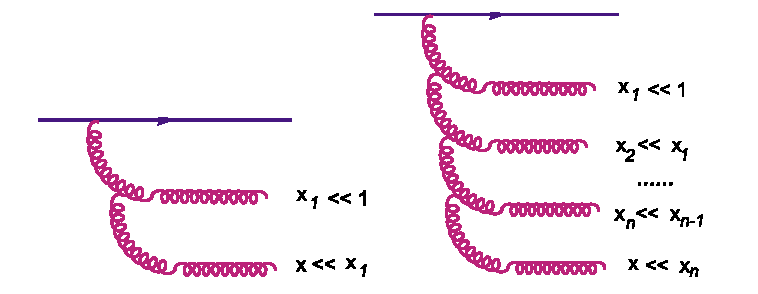
\includegraphics[width=0.7\textwidth]{figures/bfkl.pdf} 
	\caption{ Graphic representation of BFKL evolution leading to high gluon densities at low-\xb. Figure taken from Ref.~\cite{Iancu:2012xa}.}	
	\label{fig:bfkllowx}
\end{figure}

% In order to better understand how to go about the search for saturation, it is useful to first discuss the tools which will be used to "see" quarks and gluons.

\FloatBarrier

\section{ Hadronic Collisions and Jets }

The DIS experiments successfully showed the scaling violation of the linearity of \ftwo\ with \qsquare\ with smaller-\xb\ and provided precise PDFs for quarks. Indirect measurements of the gluon distribution from \ftwo\ data were still carried out, but the precision on \gx\ was limited because the photon cannot couple with gluons. Fortunately, collisions involving hadrons with hadrons, or hadrons with heavy ions open up the possibility of a hard scattering via gluon, analogous to the interaction via photon in DIS. Since gluons can couple to other gluons, hadronic collisions can be used as direct probes of \gx, providing measurements of the gluon distribution with much higher precision than in DIS. In a collision between two protons, modelled $P_{A} + P_{B} \rightarrow q_{1} + q_{2}$ and shown in the left of Fig.~\ref{fig:hadroniccollisions}, the cross section for a hard scattering process can be written~\cite{qcdbook}

\begin{equation}
\sigma(P_{1}, P_{2}) = \sum_{i,j}^{}\int_{}^{}dx_{1}dx_{2}f_{i}(x_{1},\mu^{2})f_{j}(x_{2},\mu^{2})\sigma_{ij}(p_{1},p_{2},\alphaS(\mu^2), \qsquare/\mu^{2}),
\end{equation}

where $P_{1}$ and $P_{2}$ are the four-momenta of the incoming protons, $p_{1}=x_{1}P_{1}$ and $p_{2}=x_{2}P_{2}$ are the four momenta of the partons participating in the interaction. The quark and gluon PDFs are $f_{i}$ and $f_{j}$, the QCD scattering cross section for partons of type $i$ and $j$ is $\sigma_{ij}$. The hard scattering scale \qsquare\ is determined experimentally and places a lower limit on the possible final state particles that are produced. As discussed previously, at sufficiently high \qsquare, \alphaS\ becomes small, and the cross section can be calculated perturbatively in a series of \alphaS. The factorization scale $\mu^{2}$ is an arbitrary parameter that places an energy threshold on what physics is considered part of the hadron wavefunction and what physics is part of the scattering process and can be considered in the hard scattering cross-section. The dependence on $\mu^{2}$ gets smaller by including more terms in the perturbative expansion of the cross section calculation (which requires more computing power). In general, the factorization scale should be chosen to be $\mu^{2} \sim \qsquare$. 

\begin{figure}
	\centering
	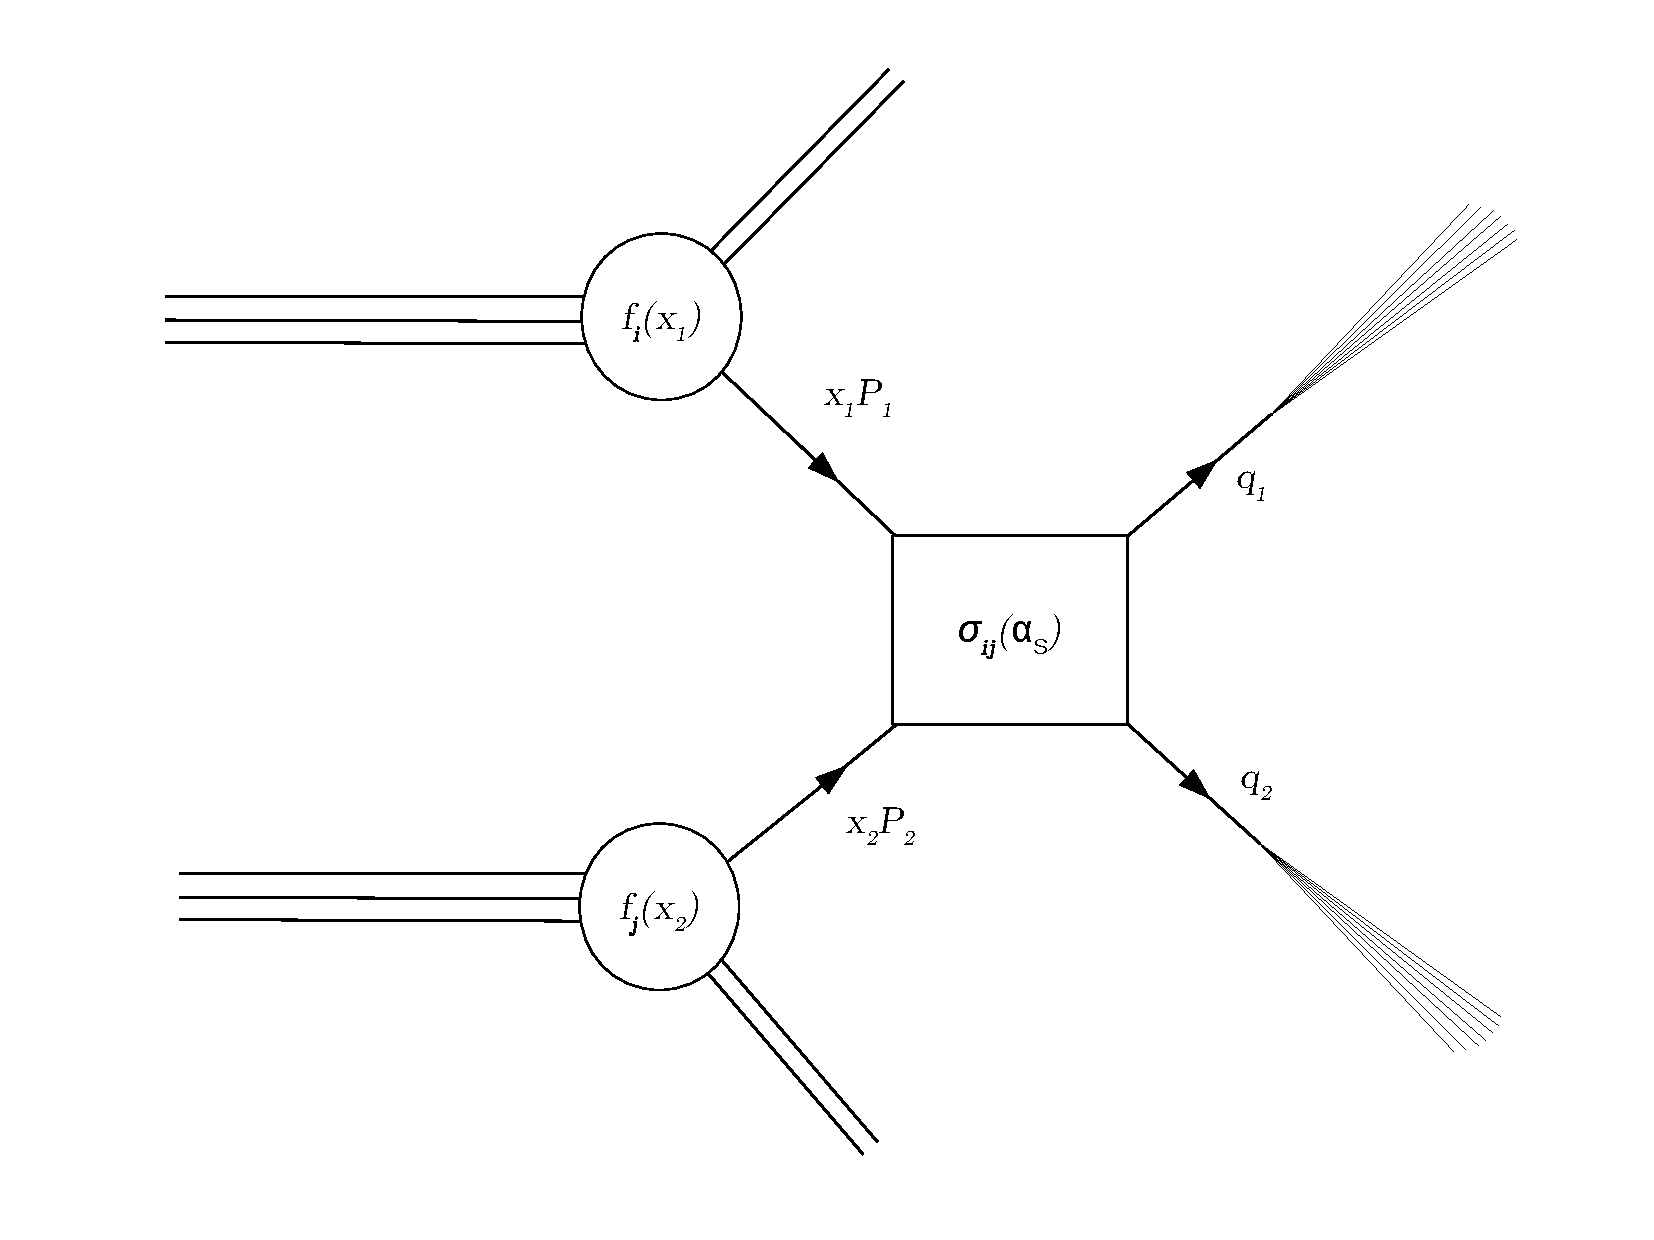
\includegraphics[width=0.7\textwidth]{figures/hadronic_collision.pdf} 
	\caption{ Diagram of a hadronic collision ($P_{A} + P_{B} \rightarrow q_{1} + q_{2}$) between two protons, producing two outgoing partons, which are represented in their final state as a stream of particles. The box represents the hard scattering process.}
	\label{fig:hadroniccollisions}
\end{figure}

A particle collision with sufficiently high energy transfer can result in a quark or gluon being ejected from the hadron in which it was confined. From the properties of confinement, a parton cannot exist alone at macroscopic distances, meaning a quark or gluon cannot be directly observed in a detector. The DGLAP formalism describes the evolution of the ejected parton from the hard scale until the perturbative limit $\lambda_{QCD}$. From QCD rules, as the distance of the exiting parton from its scattering event begins to increase, the probability for radiating collinear gluons will increase. These radiated gluons can in turn split into quark antiquark pairs, which can radiate more gluons, and so fourth. The quarks and antiquarks from the resulting cascade then recombine into color singlet states of particles  collienar with the original parton.  This process, known as $hadronization$, produces a narrow cone of particles called $jets$~\cite{Sterman:1977wj, Webber:1983if, Andersson:1983ia}. The creation of these final state particles that make up a jet is described by phenomenological models, since at every level in the hadronization process, the energy of the newly created partons decreases until perturbative methods can no longer be applied. Many of these newly created particles have a lifetime sufficiently long enough for them to reach and create a signal in a detector. In this sense, a jet is a manifestation of a parton that was knocked out in a scattering event, however the precise definition of a jet depends on the procedure with which it is reconstructed. An example of an actual event from ATLAS where two jets (dijets) were created and reconstructed is shown in Fig.~\ref{fig:atlasjets}.

\begin{figure}
	\centering
	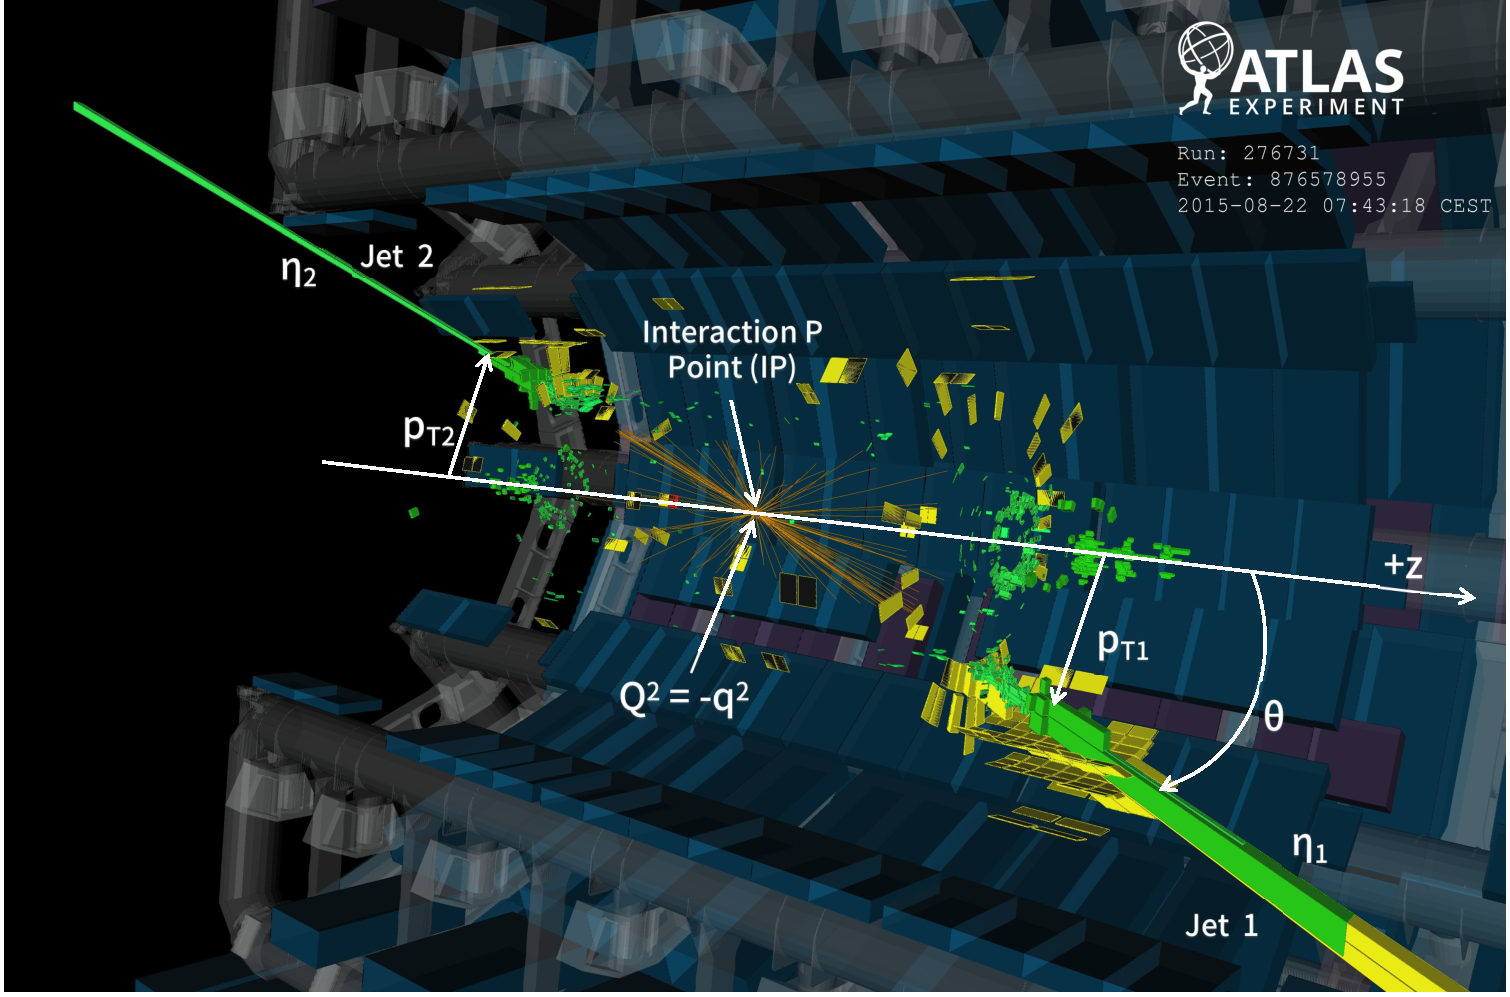
\includegraphics[width=0.7\textwidth]{figures/jets.pdf} 
	\caption{ Event display from a real ATLAS dijet event. Shown are two back-to-back jets, which are manifestations of the quarks involved in a hard scattering at the interaction point, which is labeled in the figure. }
	\label{fig:atlasjets}
\end{figure}


\subsection{\mbox{Anti-\kt} Jets} 
Before a jet's energy and position can be correctly described, a prescription of what a jet is must be agreed upon. A jet can have many constituents, which are final state particles produced in the hadronization process. These particles can be physically detected and used as input into clustering algorithms that aim to describe jets consistent with theory predictions~\cite{Ellis:1993tq,Dokshitzer:1997in,Wobisch:1998wt,Blazey:2000qt}. While different algorithms have their advantages and disadvantages, the \antikt\ algorithm~\cite{Cacciari:2008gp} has grown in popularity since its introduction almost a decade ago. Besides its fast computation speed, the main advantage of the \antikt\ algorithm is its infrared and collinear safety (IRC) from effects of soft radiation.

Any jet clustering algorithm needs to accept a set of homogeneous input data (objects) such as the four-momenta of particles, calorimeter tower energies, topological calorimeter cells, etc. The treatment of these input objects by the algorithm is identical. The \antikt\ algorithm comes from a broader family of \kt\ clustering algorithms that appear the same in their formalism but yield different results based on an important parameter that will be discussed shortly. The general form of any \kt\ algorithm involves a collection of input objects with indexes $i$ having energy and spatial coordinates $(\eta_{i}, \phi_{i}, p_{\mathrm{T}_{i}})$ where $\eta_{i}$, $\phi_{i}$, and $\pt_{i}$ are the objects pseudorapitidy, azimuthal angle, and transverse momentum, respectively. Between any two objects $i$ and $j$, two distances are defined in terms of energy and position:

\begin{equation}
	d_{iB} = -p^{2p}_{\mathrm{T}_{i}}
	\label{diB}
\end{equation} 
\begin{equation}
	d_{ij} = min( p^{2p}_{\mathrm{T}_{i}}, p^{2p}_{\mathrm{T}_{j}})\frac{\Delta R}{R^{2}}
	\label{dij}
\end{equation}

where $\Delta R^{2} = (\eta_{i} - \eta_{j} )^2 - ( \phi_{i} - \phi_{j} )^2$, $R$ is the characteristic radius parameter describing the maximum allowed radius of a jet, and the parameter $p$ is what determines which type of \kt\ algorithm is used. The general prescription for any \kt\ algorithm is as follows:

\begin{enumerate}
	\item Out of the list of objects, calculate all distances $d_{ij}$ and $d_{iB}$.
	\item Identify the smallest distance out of $d_{ij}$ and $d_{iB}$.
	\item If the minimum is $d_{ij}$, combine the four-momenta of the $i^{th}$ and $j^{th}$ objects, return to the first step, and begin again.
	\item If the minimum is $d_{iB}$, save object $i$ as a jet and remove it from the list of objects. Then return to the first step and begin again.
	\item Continue this process until the list of objects is empty.
\end{enumerate}

The behavior of all the \kt\ algorithms with respect to soft radiation is the same for any $p < 0$ but the focus is going to be on the case of $p = -1$, which is the parameter used in the \antikt\ jet reconstruction algorithm mentioned earlier. To understand the general idea of how it works, it is useful to begin with an ensemble several high \pt\ (hard) objects, and many low \pt\ (soft) objects used as an input to the algorithm. The distance $d_{ij}$ between a hard particle $i$ and a soft particle $j$ will dominated by the hard particle $i$ and will be smaller than the distance $d_{kl}$ between two soft particles $k$ and $l$. This means that soft objects will cluster with hard objects preferentially over other soft objects. If the hard object $i$ has no other hard object within a distance of $2R$, all soft objects within a circle of radius $R$ will simply cluster with object $i$ and eventually form a perfectly conical jet of radius $R$. If there are two had particles with $\Delta R < R$, then they will be combined to form a jet of radius $R$ around the higher \pt\ object. If object $i$ has another hard object within $R < \Delta R < 2R$, the object with higher \pt\ will form a perfectly conical jet of radius R, and the object with lower \pt\ will form a jet an area clipped by its neighbor with higher \pt. In reality, it does not matter what object is hard or soft, the algorithm takes a list of objects as input, naturally performs the clustering of these objects according to its prescription, and outputs a collection of jets. An example of the same input data run through different jet reconstruction algorithms is shown in Fig~\ref{fig:jetalgos}. The \antikt\ algorithm was adopted by ATLAS as a standard way to describe jets due to its IRC safety, fast performance, and robust treatment of various kinds of input datasets. 

\begin{figure}
	\centering
	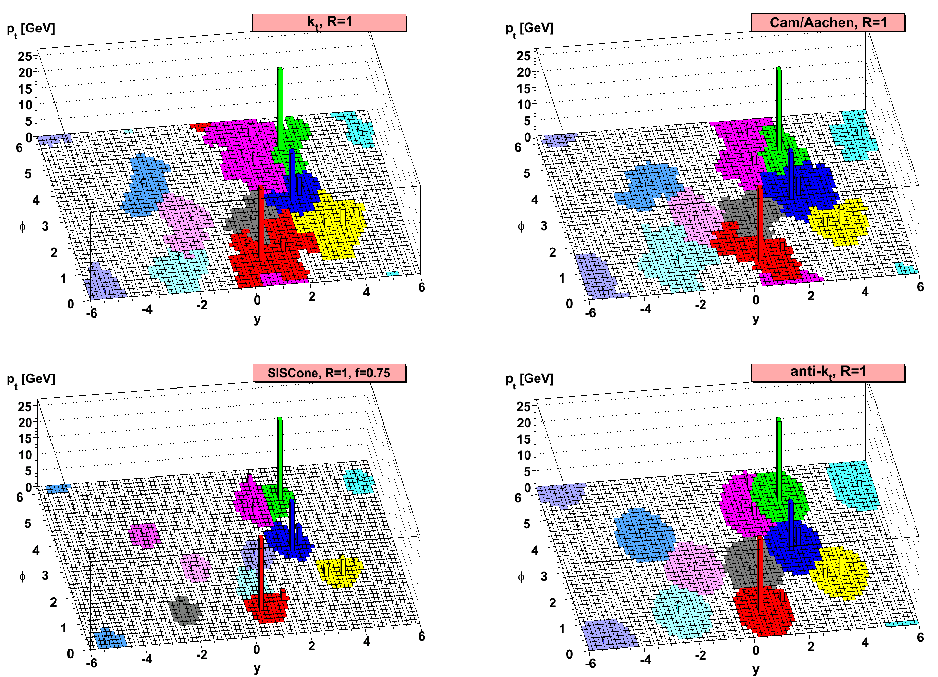
\includegraphics[width=0.75\textwidth]{figures/jetalgo.pdf} 
	\caption{ Results of jet reconstruction by the \kt\ (top left), Cambridge Aachen (top right), SISCone (bottom left), and \antikt\ (bottom right) algorithms on identical input sets with a jet radius requirement of \ROne. Figure taken from Ref.~\cite{Cacciari:2008gp}.}
	\label{fig:jetalgos}
\end{figure}

\FloatBarrier

\section{Gluon Saturation}
The search for the onset of saturation was first pursued with $d+\mathrm{Au}$ collisions at RHIC~\cite{Adler:2003au, Wang:2007zv, Adare:2011sc}, where the sensitivity to possible saturation effects was increased due to the enhancement of the nuclear gluon density in the Lorentz-contracted heavy ion nucleus~\cite{Albacete:2014fwa,Blaizot:2016qgz}. More recent measurements at the LHC have been performed in the proton-going direction of \pPb\ collisions and at higher center-of-mass energies, allowing lower-\xb\ of the lead nucleus to be probed~\cite{ATLAS:2014cpa, Adam:2015xea, Adam:2015hoa, Khachatryan:2016xdg}. The ALICE measurement of dijet azimuthal correlations at mid-rapidity did not find significant modification in \pPb\ collisions compared to \pp\ collisions. The ATLAS and CMS measurements of inclusive jet production also did not find significant evidence of nuclear modification. Recently, CMS extended the search for gluon saturation to the highest gluon densities reached so far by measuring the inclusive jet cross-section in \pPb\ collisions at very forward rapidity using the CASTOR detector with $-6.6 < \eta < -5.2$, probing $x$ down to $10^{-6}$~\cite{VanDeKlundert:2017ulj}. Comparing measured jet \pt\ spectra to event generators (\textsc{Epos-lhc}~\cite{PhysRevC.92.034906}, \textsc{Hijing}~\cite{PhysRevD.44.3501}, and \textsc{Qgsjetii-04}~\cite{qgsjet}), it was found that none could describe the data over the full jet \pt\ spectra range, opening up the possibility for nuclear effects not described by these models. Currently, the differences between nuclear PDFs (nPDFs) and free nucleon PDFs are often understood from shadowing, anti-shadowing, and EMC effects~\cite{Eskola:2016oht,Kovarik:2015cma}. Calculating nPDFs  $f_{i}^{A}( \xb, \qsquare )$ for parton types $i$ from $F_{2}^{A}$ of heavy ions with atomic number $A$ and comparing them to free nucleon PDFs $f_{i}^{p}( \xb, \qsquare )$ calculated from $F_{2}^{p}$ is direct measure of the nuclear modification factor

\begin{equation}
	R^{A}_{i} = \frac{f_{i}^{A}( \xb, \qsquare )}{A f_{i}^{p}( \xb, \qsquare )}.
\end{equation}

Studies of nPDFs in heavy ion nuclei expected a scaling of free nucleon PDFs with $A$ such that the nuclear modification factor is consistent with unity. The parameterization of $R_{i}^{A}$ shown in Fig~\ref{fig:shadowing} indicates that the nuclear modification factor is not consistent with unity at various values of \xb. The suppression of $R^{A}_{i}$ can be seen from shadowing (low-\xb) and EMC($\xb~\sim 1$) effects, while enhancement of $R^{A}_{i}$ can be seen from the antishadowing effect at $\xb~\sim 10^{-1}$. The shadowing effect, which is of most interest to the low-\xb\ physics of this thesis, is thought to arise from screening of the nuclear parton densities by gluons on the outside of the heavy ion nucleus, which interact preferentially with any incoming probes. While this effect is not completely understood, it is well known experimentally. As discussed earlier, the large uncertainty on the gluon nPDFs and free nucleon gluon PDFs is due to the inability to directly probe gluon densities from \ftwo. Additionally, final state processes can also contribute to the modification of the gluon nPDF. This opens up the possibility for additional nuclear processes to contribute to the gluon density suppression at low-\xb.

\begin{figure}
	\centering
	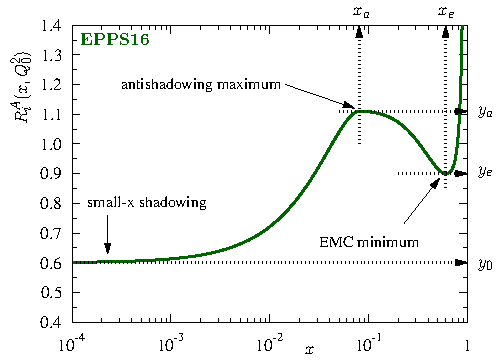
\includegraphics[width=0.7\textwidth]{figures/shadowing.pdf} 
	\caption{ Illustration of a generalized EPPS16 parameterization of the nuclear modification factor $R^{A}_{i}$ for different parton types $i$ and heavy ions with atomic number $A$. Suppression of $R^{A}_{i}$ by nuclear shadowing and EMC effects are prevalent at low- and high-\xb. Enhancement of $R^{A}_{i}$ due to antishadowing effects are seen in an intermediate-$x$ range. Figure taken from Ref.~\cite{Eskola:2016oht}. }	
	\label{fig:shadowing}
\end{figure}

\FloatBarrier
\section{Color Glass Condensate}

One of the proposed models of gluon saturation is in the framework of the Color Glass Condensate (CGC)~\cite{Iancu:2002xk, Kharzeev:2004bw, Gelis:2012ri}. It is useful to discuss the meaning of the name: $color$ comes from the fact that gluons carry a color charge, $glass$ describes how short lived gluons with low-\xb\ see the surrounding higher-\xb\ gluons in the dense medium as "frozen", $condensate$ describes the saturated nature of the high density gluons recombining with one another. The CGC effective theory describes a model for the interaction of a high energy parton with a highly dense gluon medium described by the BFKL evolution that includes a non-linear term responsible for gluon recombination. In the schematic shown in Fig.~\ref{fig:cgcfield}, a low-\xb\ gluon that originated or re-scattered from other gluons with higher $x' > \xb$ is emitted and interacting with this gluon is a probe of the overall gluon field $A(\rho)$, where $\rho$ is the color charge density of the nucleon. Recently, together with non-relativistic QCD, the CGC model was able to successfully describe experimental data on the cross section of $J/\psi$ production at ALICE~\cite{Weber:2017kjj}, shown in Fig.~\ref{fig:jpsialice}.

%single model for a many body self-interacting system of highly dense gluons

\begin{figure}
	\centering
	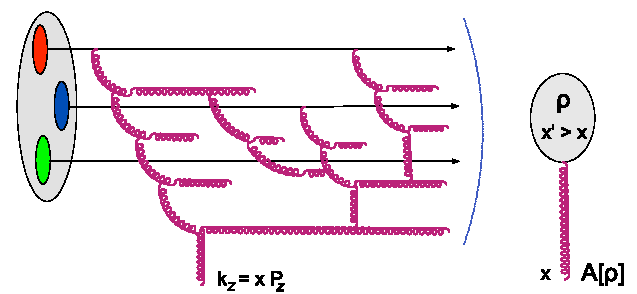
\includegraphics[width=0.65\textwidth]{figures/cgc_field_2.pdf} 
	\caption{ Schematic representation of the CGC theory, showing the high density, low-\xb\ gluons originating from high-\xb\ partons (left). These gluons form a gluon field $A{\rho}$ where the whole gluons with higher-\xb\ are represented by a color charge density $\rho$. Figure taken from Ref.~\cite{Iancu:2012xa}. }	
	\label{fig:cgcfield}
\end{figure}


\begin{figure}
	\centering
	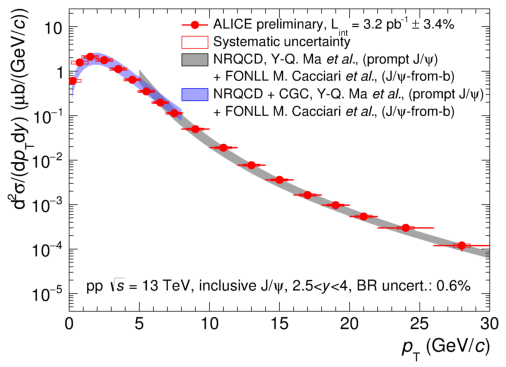
\includegraphics[width=0.65\textwidth]{figures/jpsialice.pdf} 
	\caption{ Figure taken from Ref.~\cite{Weber:2017kjj}. }	
	\label{fig:jpsialice}
\end{figure}

A measurement probing gluon saturation in nuclear gluon densities in the framework of the CGC model was  was proposed by measuring possible modifications of dijet azimuthal angular distributions in \pPb\ and \pp\ collisions at an $x$ down to $10^{-5}$~\cite{vanHameren:2014lna,}. For back-to-back dijets, the gluon field in the Pb nucleus is probed at low transverse momentum where saturation effects are expected to be large. These effects are described by whether or not an incoming parton scatters individually off each gluon in the highly dense field of the lead nucleus, or recoils against the nucleus as a whole. An away-side jet is created when a constituent gluon of this dense field is knocked out of the nucleus by the scattering incoming parton. However, due to the highly dense field, the incoming parton can scatter many times, losing energy and changing trajectory. As a result, if there are two outgoing jets, one from the scattered parton, and the other jet (away side) from a knocked out gluon, they may not be perfectly back-to-back, resulting in the azimuthal broadening. The monojet signature could result from the incoming parton recoiling off the nucleus coherently~\cite{Kharzeev:2004bw}. The parton would not scatter with any of the individual partons, and as a result, would not produce an away-side jet. To probe these effects, one must define some observables, which will be extracted from data and presented in the latter sections of this thesis.

\section{Measured Observables}

This thesis will present a  measurement of dijet production at forward rapidity with the ATLAS detector. Proton-lead collisions are studied in addition to proton-proton collisions because of the enhancement of gluon densities in the Lorentz contracted lead nucleus.


At the leading order, in a hard scattering event between a proton moving in the $+z$ direction, and a lead nucleus moving in the $-z$ direction, as shown in the middle panel of Fig.~\ref{fig:yandystar}, there will be two outgoing partons, one with transverse momentum \ptone\ and center-of-mass rapidity \ystarone\ coming from the proton, and one with transverse momentum \pttwo\ and center-of-mass rapidity \ystartwo\ coming from a nucleon in the lead ion. The center-of-mass rapidities ($\ystar \equiv y - \Delta y$) are used to account for the rapidity shift of the center-of-mass frame of the \pPb\ system relative to the ATLAS laboratory frame. The resulting expressions for parton momentum fractions $x_{p}$ of the proton's parton, and $x_{\mathrm{Pb}}$ of a lead nucleon's parton will be:

\begin{equation}
x_{p}=\frac{\ptone e^{\ystarone}+\pttwo e^{\ystartwo}}{\sqrt{s}}, \ \ x_{\mathrm{Pb}}=\frac{\ptone e^{-\ystarone}+\pttwo e^{-\ystartwo}}{\sqrt{s}}.
\label{eqn:x1x2}
\end{equation}

From these equations, it is clear that to probe a lower $x_{\mathrm{Pb}}$, two forward (high \ystarone and \ystartwo) particles, with low \ptone\ and \pttwo\ are preferred. To show the difference between rapidity $y$ and center-of-mass rapidity \ystar, an event producing two jets in \pp\ collisions is shown on the left panel of Fig.~\ref{fig:yandystar}. The azimuthal angle \Dphi\ between two jets is shown on the right panel of  Fig.~\ref{fig:yandystar}

\begin{figure}
	\centering
	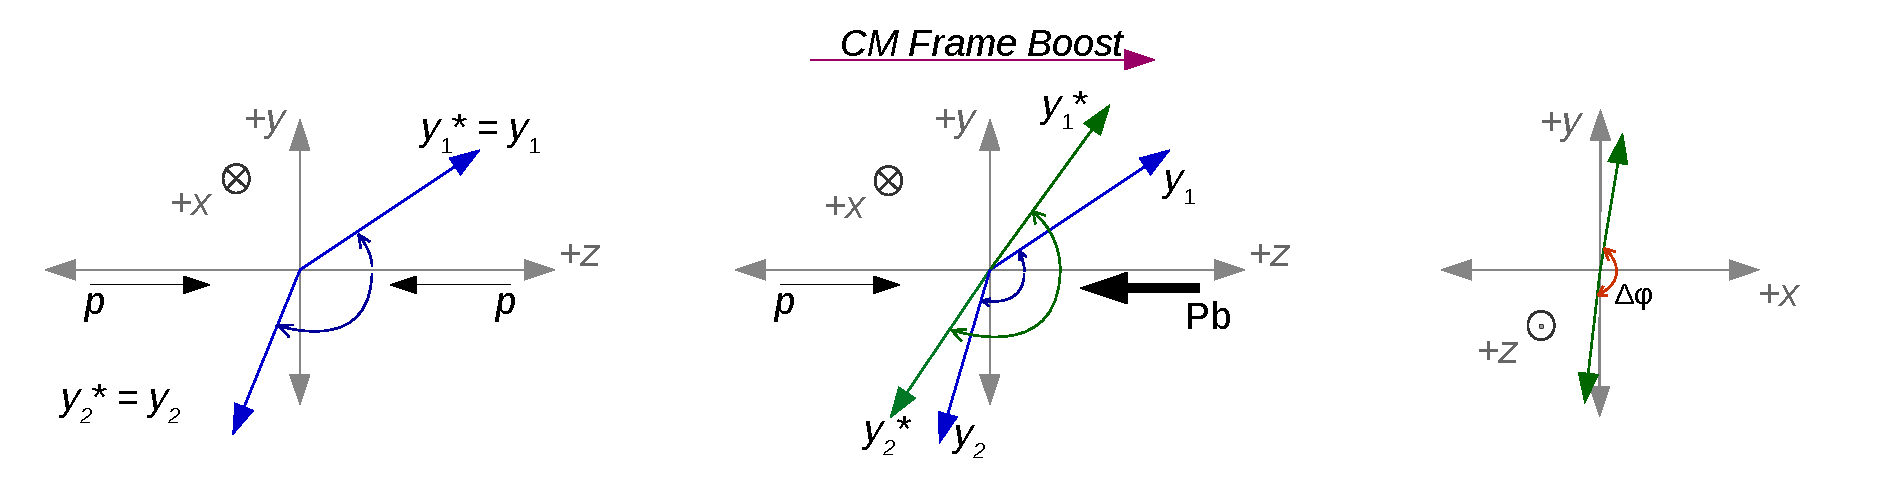
\includegraphics[width=0.970\textwidth]{figures/collision_system.pdf} 
	\caption{Example of a collision in the $y-z$ plane in \pp\ where $y=\ystar$ (left), a collision in the $y-z$ plane in \pPb\ where $\ystar \equiv y - \Delta y$ (middle) to account for the boost ($\Delta y$) of the center-of-mass system, and a collision in the $x-y$ plane showing the difference in azimuthal angle \Dphi\ between two jets (right). }	
	\label{fig:yandystar}
\end{figure}

\begin{figure}
	\centering
	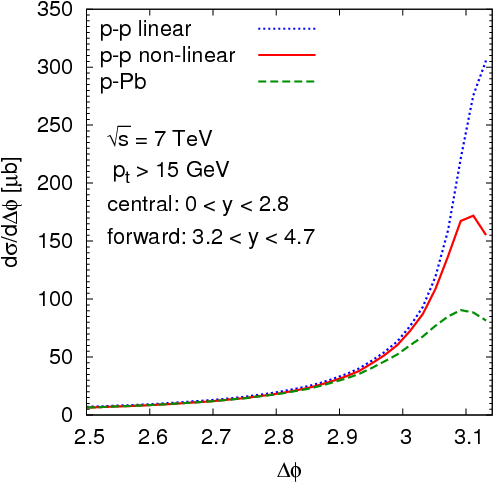
\includegraphics[width=0.40\textwidth]{figures/kutak0.png} 
	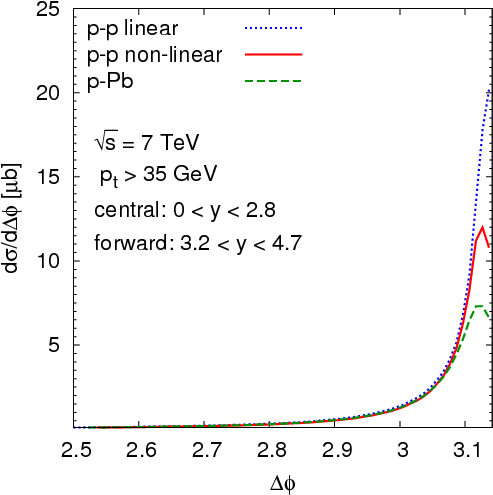
\includegraphics[width=0.40\textwidth]{figures/kutak1.png} 
	\caption{ Dijet azimuthal angular correlations from theoretical models for central-forward \pp\ and \pPb\ collisions as a function of \Dphi\ between two jets in different \pt\ bins. Figure taken from Ref. ~\cite{Kutak:2012rf}. }	
	\label{fig:kutakdphi}
\end{figure}

The final observables in this analysis are dijet azimuthal angular \Dphi\ distribution widths and conditional yields of dijets.  Example dijet \Dphi\ distributions are shown from theoretical models in Figure~\ref{fig:kutakdphi}. The measurement is performed in different intervals of \ystarone, \ystartwo, \ptone, and \pttwo, where \ystarone, \ptone\ is the center-of-mass rapidity and transverse momentum of the leading jet, and \ystartwo, \pttwo\ the  center-of-mass rapidity and transverse momentum of the sub-leading jet. The leading jet, which is required to be in the forward (defined as proton-going) direction, has the highest \pT\ in the event, and the sub-leading jet has the second highest \pT\ in the event. This is a measurement of dijets probing the lowest-\xb\ of the lead nucleus at the hardest scattering scale so far. The azimuthal angular correlation functions, \conetwo, which are normalized to the number of leading jets, are defined as

\begin{equation}
\conetwo=\frac{1}{N_{1}} \frac{\mathrm{d}N_{12}}{\mathrm{d}\Dphi},
\label{eqn:c12}
\end{equation}

where $N_{1}$ is the number of leading jets, $N_{12}$ is the number of dijets, and \Dphi\ is the lower azimuthal angle between the leading and sub-leading jets. The \conetwo\ distributions are fitted and their widths \wonetwo\ defined by the root-mean-square (RMS) of the fit: \wonetwo = RMS(\conetwo).

In addition to dijet azimuthal angular distributions, the dijet conditional yields, \ionetwo, are measured and defined as

\begin{equation}
\ionetwo=\frac{1}{N_{1}}  \frac{\mathrm{d}N_{12}}{\mathrm{d}\ystarone\mathrm{d}\ystartwo\mathrm{d}\ptone\mathrm{d}\pttwo}.
\label{eqn:ippb}
\end{equation}

where \ptone, \pttwo, \ystarone, and \ystartwo\ are the transverse momenta and center-of-mass rapidities of the leading and sub-leading jets, respectively. 

The azimuthal angular correlations and conditional yields evaluated in \pPb\ and \pp\ collisions are compared and the ratios in \wonetwo\ and \ionetwo\ between the two systems are calculated as:

\begin{equation}
\cppb=\frac{W_{12}^{\pPb}}{W_{12}^{\pp}} \ \ , \ \ \ippb=\frac{I_{12}^{\pPb}}{I_{12}^{\pp}}.
\end{equation}

Finding a broadening in the dijet angular correlation distribution for \pPb\ collisions compared to \pp\ collisions probes for nuclear effects in the jet formation and scattering off individual gluons of the highly dense gluon field. A suppression of the conditional yields in \pPb\ compared to \pp\ could be an indicator of the mono-jet or jet quenching event signature due to the coherent scattering off the lead nucleus as a whole.

To closer follow next-to-leading-order (NLO) calculations, a minimum $\Delta \pT=\ptone - \pttwo$ is required on the dijets~\cite{Potter:1999gg,Klasen:1995xe,Frixione:1997ks}. However, techniques such as Sudakov re-summation~\cite{Bury:2017jxo} can take into account the absence of $\Delta \pT$ requirements. Also, comparisons with fixed-order calculations and soft gluon re-summation, which involve transverse momentum dependent PDFs, instead of collinear PDFs, are better suited for scenarios not requiring any minimum $\Delta \pT$ cut. The results of the measurement are therefore presented both without any requirement on $\Delta\pT$, as well as with the requirement of $\Delta\pT>3$ GeV.

\FloatBarrier

%%%%%%%%%%%%%%%%%%%%%%%%%%%%%
%\chapter{ATLAS Required Qualification Work}
%\label{sec:qualification}
%% !TEX root = thesis-ex.tex


To gain authorship in the ATLAS collaboration, one has to contribute towards ATLAS technical work. My qualification task was to derive the cross calibration heavy ion jets and the related uncertainties. The aim of the cross calibration procedure, first described in \cite{xcalib_run1} is to use jets constructed by the \pp\ jet reconstruction algorithm (EMTopo jets) \cite{Aad:2014bia, Aad:2011he, Aaboud:2017jcu} to calibrate jets reconstructed using the heavy ion reconstruction algorithm (HI jets) discussed in \cite{Aad:hi_jets}.

Deriving and applying this calibration was vital to all Run 2 heavy ion jet analyses from ATLAS \cite{PhysRevC.98.024908, 201865, 2019108, 2019108, 2019167}.


\section{Introduction}
\label{sec:qual_intro}
%-------------------------------------------------------------------------------

The performance of the EMTopo jets is well understood in\ \pp \ collisions \cite{Aad:2014bia} \cite{Aad:2011he}. The goal of the cross calibration procedure, first described in \cite{xcalib_run1} is to use these jets to calibrate the HI jets, that are reconstructed using the HI reconstruction algorithm discussed in \cite{Aad:hi_jets}. On average, the\ \pt \ of the HI jets is expected to differ from the EMTopo jets due to the differences in the reconstruction algorithm, and the insitu corrections that are applied to to the latter. The insitu corrections cannot directly be derived for heavy ions because of the high multiplicity, but comparing the HI and EMTopo jets in data and MC and scaling the HI jets with the ratio of $\langle \pt ^\hi / \pt^\emt \rangle$ in data and MC allows the application of EMTopo insitu corrections to HI jets \cite{xcalib_run1}

%-------------------------------------------------------------------------------
\section{Datasets and Event Selection}
\label{sec:qual_datasets}
%-------------------------------------------------------------------------------
The data used in the cross calibration study was obtained in the 2015 13 TeV run, and the MC was generated as part of the MC15 period C. A list of the datasets is given in Table~\ref{table:datasets}.



\begin{table}[ht]
\tiny
\caption{List of datasets}
\centering
\begin{tabular*}{\textwidth}{l @{\extracolsep{\fill}} ll}
\hline\hline
Datasets & \#Events [Millions] \\  % inserts table %heading
\hline
group.phys-hi.data15\_13TeV.ZeroBias.merge.AOD.p2634.2016HIPAOD & 12M \\
group.phys-hi.data15\_13TeV.express\_express.merge.AOD.p2634.2016HIPAOD & 2M \\
mc15\_13TeV.361021.Pythia8EvtGen\_A14NNPDF23LO\_jetjet\_JZ1W.merge.AOD.e3569\_s2832\_r7968\_p2686 & 2M \\
mc15\_13TeV.361022.Pythia8EvtGen\_A14NNPDF23LO\_jetjet\_JZ2W.merge.AOD.e3668\_s2832\_r7968\_p2686 & 2M \\
mc15\_13TeV.361023.Pythia8EvtGen\_A14NNPDF23LO\_jetjet\_JZ3W.merge.AOD.e3668\_s2832\_r7968\_p2686 & 2M \\
mc15\_13TeV.361024.Pythia8EvtGen\_A14NNPDF23LO\_jetjet\_JZ4W.merge.AOD.e3668\_s2832\_r7968\_p2686 & 2M \\
mc15\_13TeV.361025.Pythia8EvtGen\_A14NNPDF23LO\_jetjet\_JZ5W.merge.AOD.e3668\_s2832\_r7968\_p2686 & 2M \\ [1ex]
\hline
\end{tabular*}
\label{table:datasets}
\end{table}


Events in data were selected based on the trigger $\eta-\phi$ map given in  Fig.~\ref{fig:TrigMap}. The HLT\_j40\_L1ZB, HLT\_j60, and the HLT\_j60\_L1RD0\_FILLED triggers were extended out to $|\eta| < 3.2 $.

%\begin{figure}
%\centering
%\begin{subfigure}[b]{\textwidth}
%    \centering
%    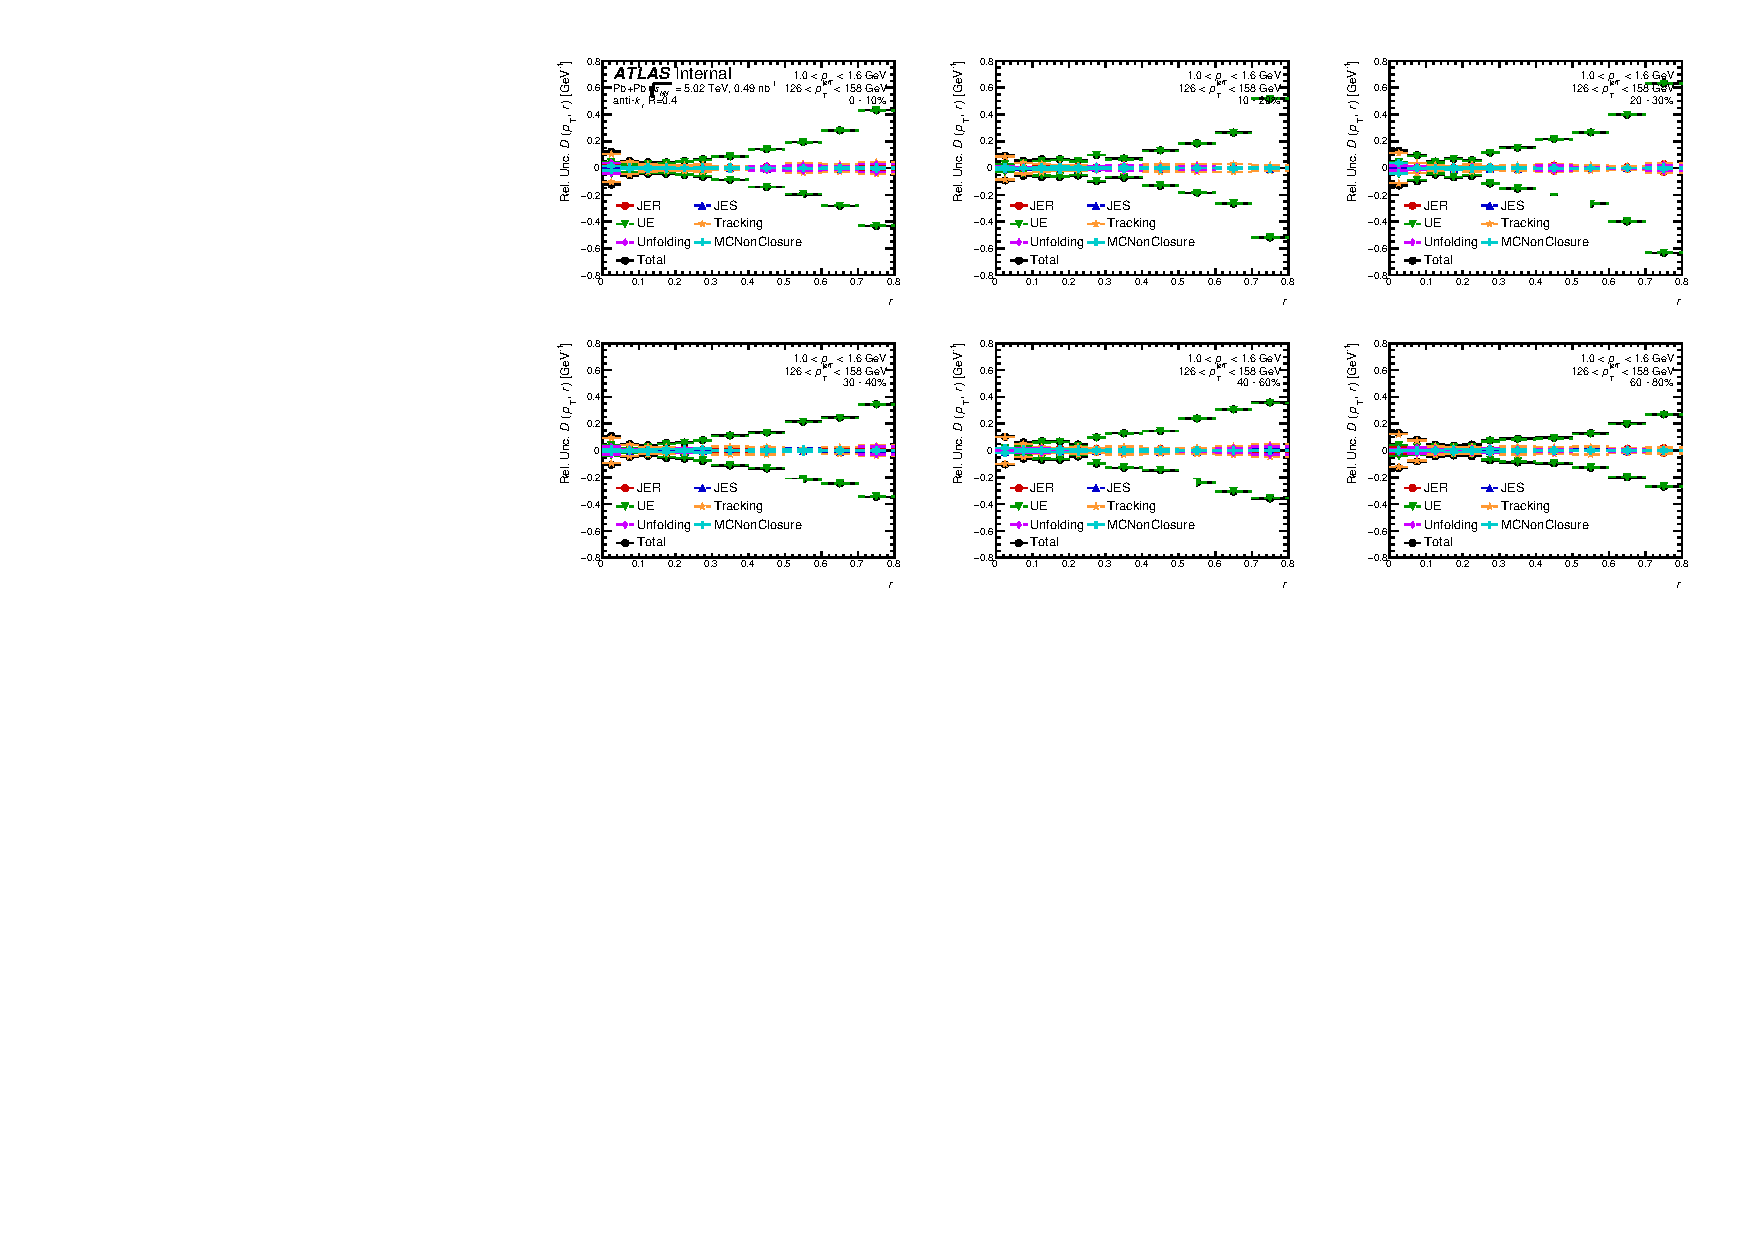
\includegraphics[page=1, width=\textwidth]{figures/main/figures_systematics/Summary_ChPS_dR_sys_PbPb_error}
%    \caption{}
%    \label{fig:rdptr_sys_uncert1a}
%\end{subfigure} \\
%\begin{subfigure}[b]{\textwidth}
%    \centering
%    \includegraphics[page=3, width=\textwidth]{figures/main/figures_systematics/Summary_ChPS_dR_sys_PbPb_error}
%    \caption{}
%    \label{fig:rdptr_sys_uncert1b}
%\end{subfigure}\hfill
%   \caption{A summary of the systematic uncertainties on \RDptr\ distributions for different track \mbox{$1.0 < \pt < 1.6$ GeV} (\ref{fig:rdptr_sys_uncert1a}) and \mbox{$2.5 < \pt < 4.0$ GeV} (\ref{fig:rdptr_sys_uncert1b}), for jets with \pt\ 126--158 \GeV\ , as a function of \rvar\ for different centrality bins. Different panels are different centrality bins. The uncertainties from the JES, JER, UE, and Tracking  are shown, along with the total systematic uncertainty from all sources. }
%\label{fig:rdptr_sys_uncert1}
%\end{figure}
%

%\begin{figure}
%	\centering
%	\subfloat[ \label{a}]{{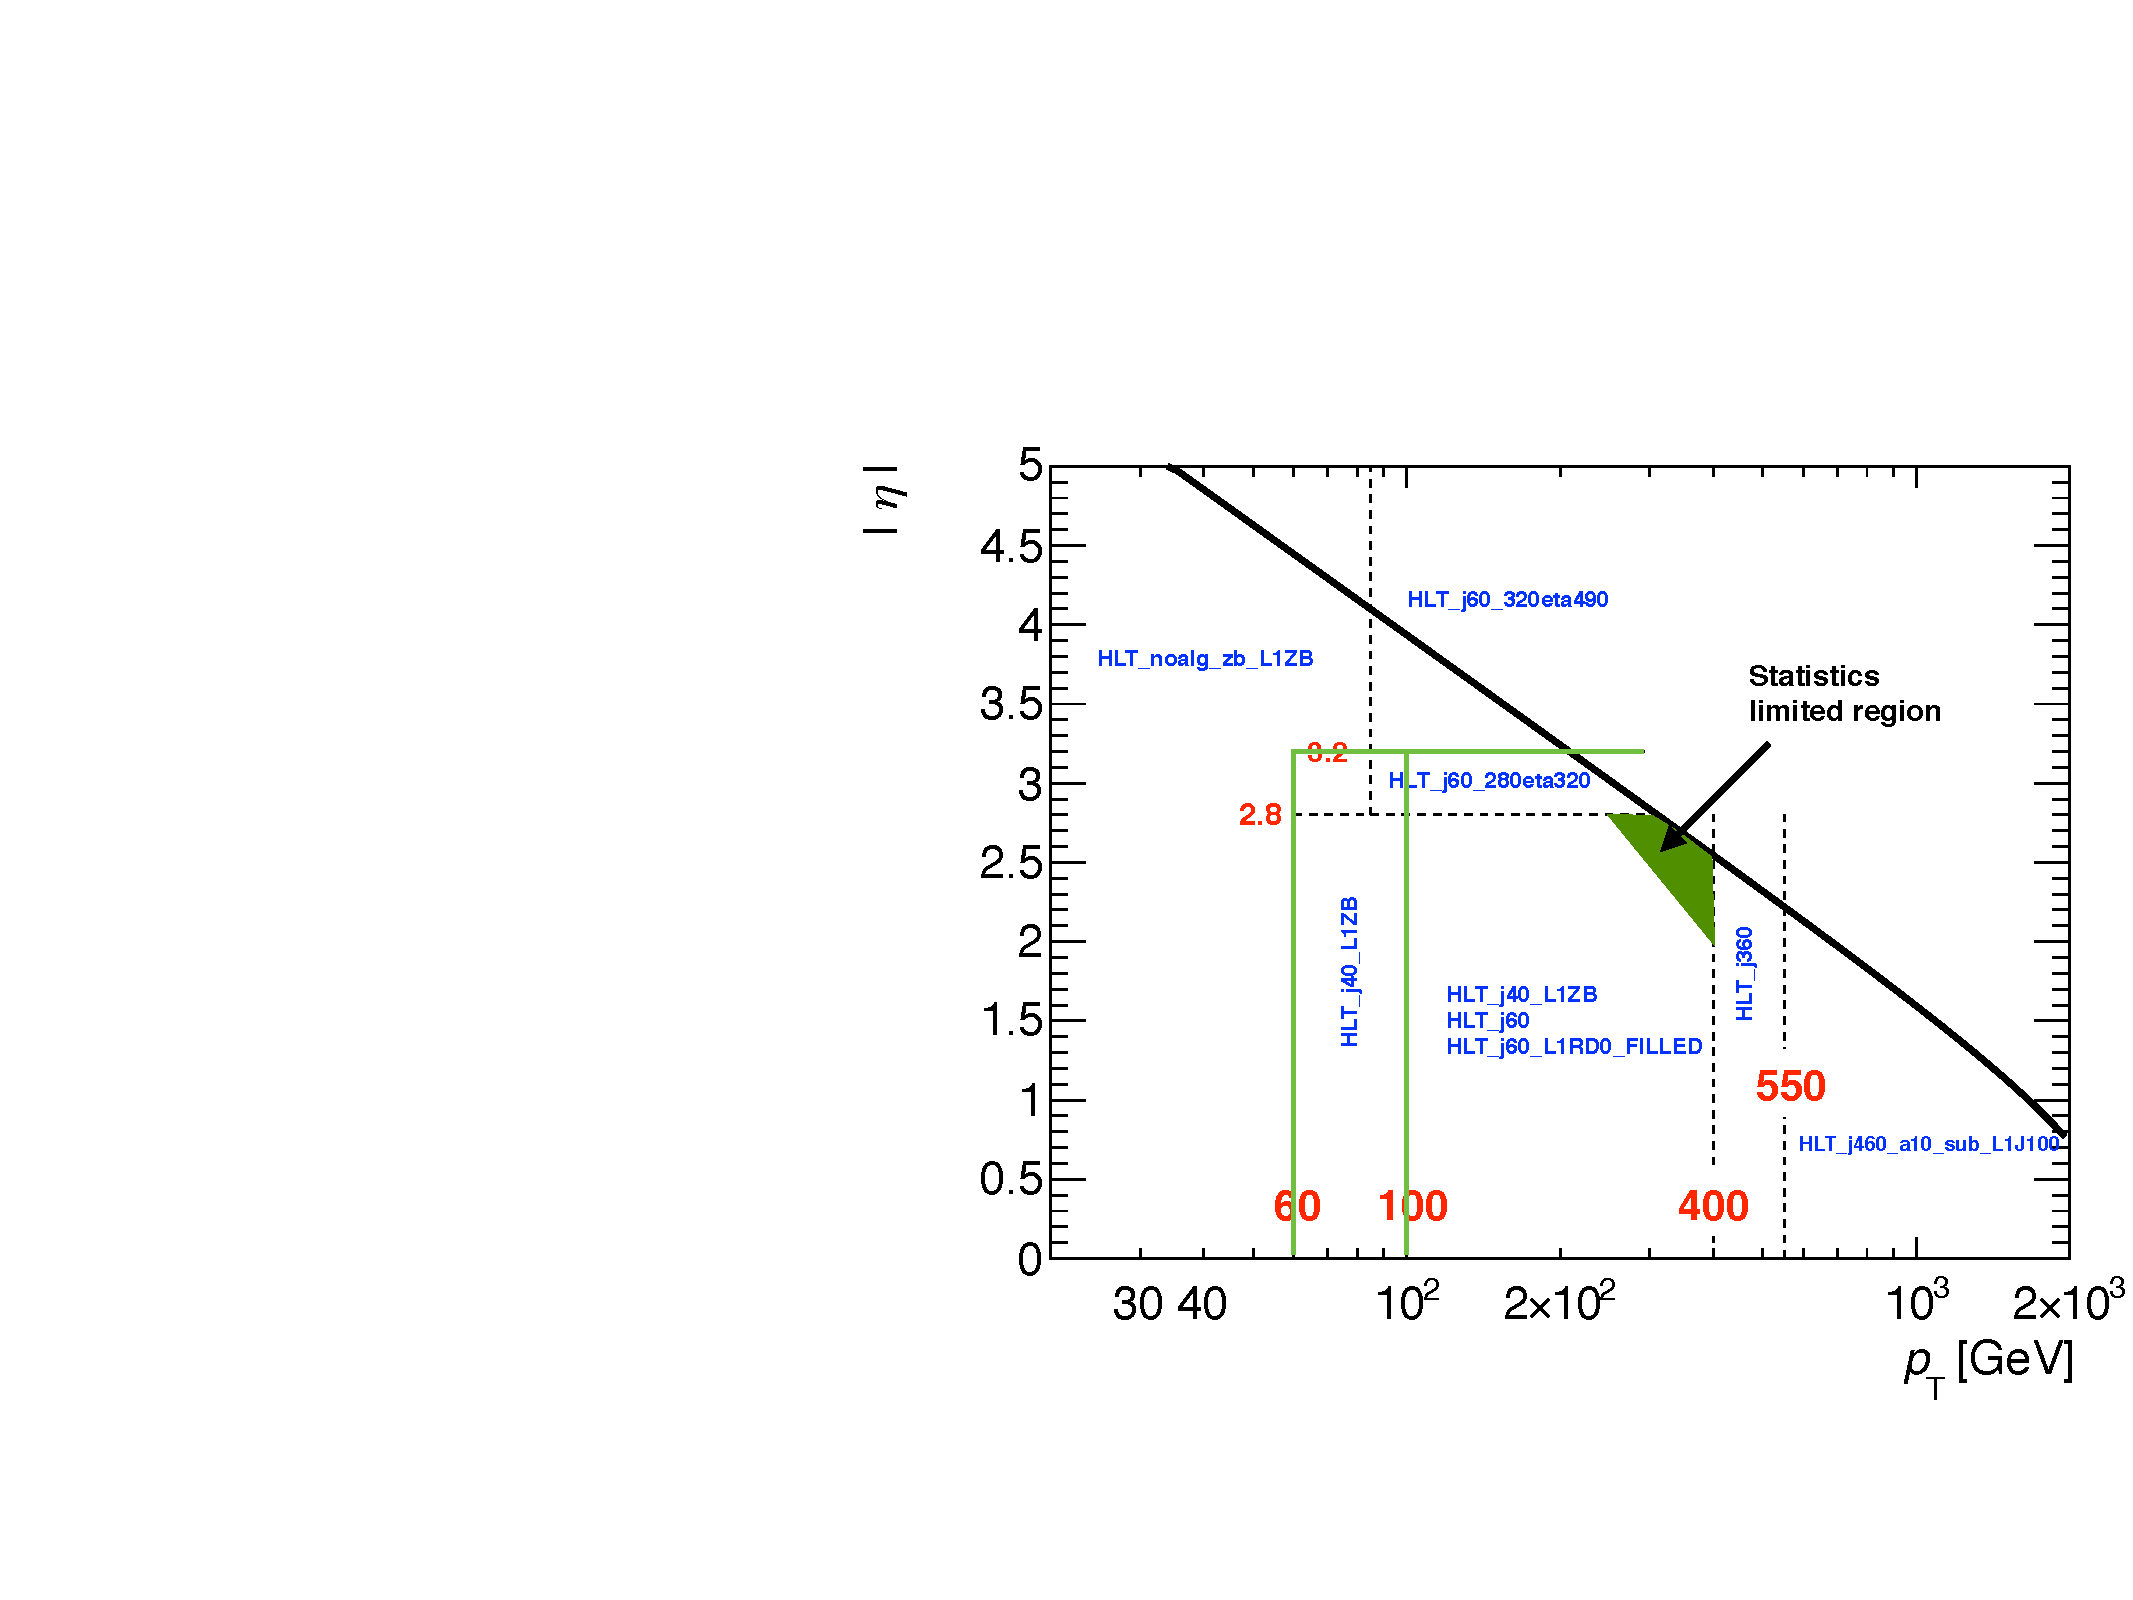
\includegraphics[width=0.5\textwidth]{figures/qualification/TrigMap.pdf} }}%
%	\subfloat[ \label{selection_2}]{{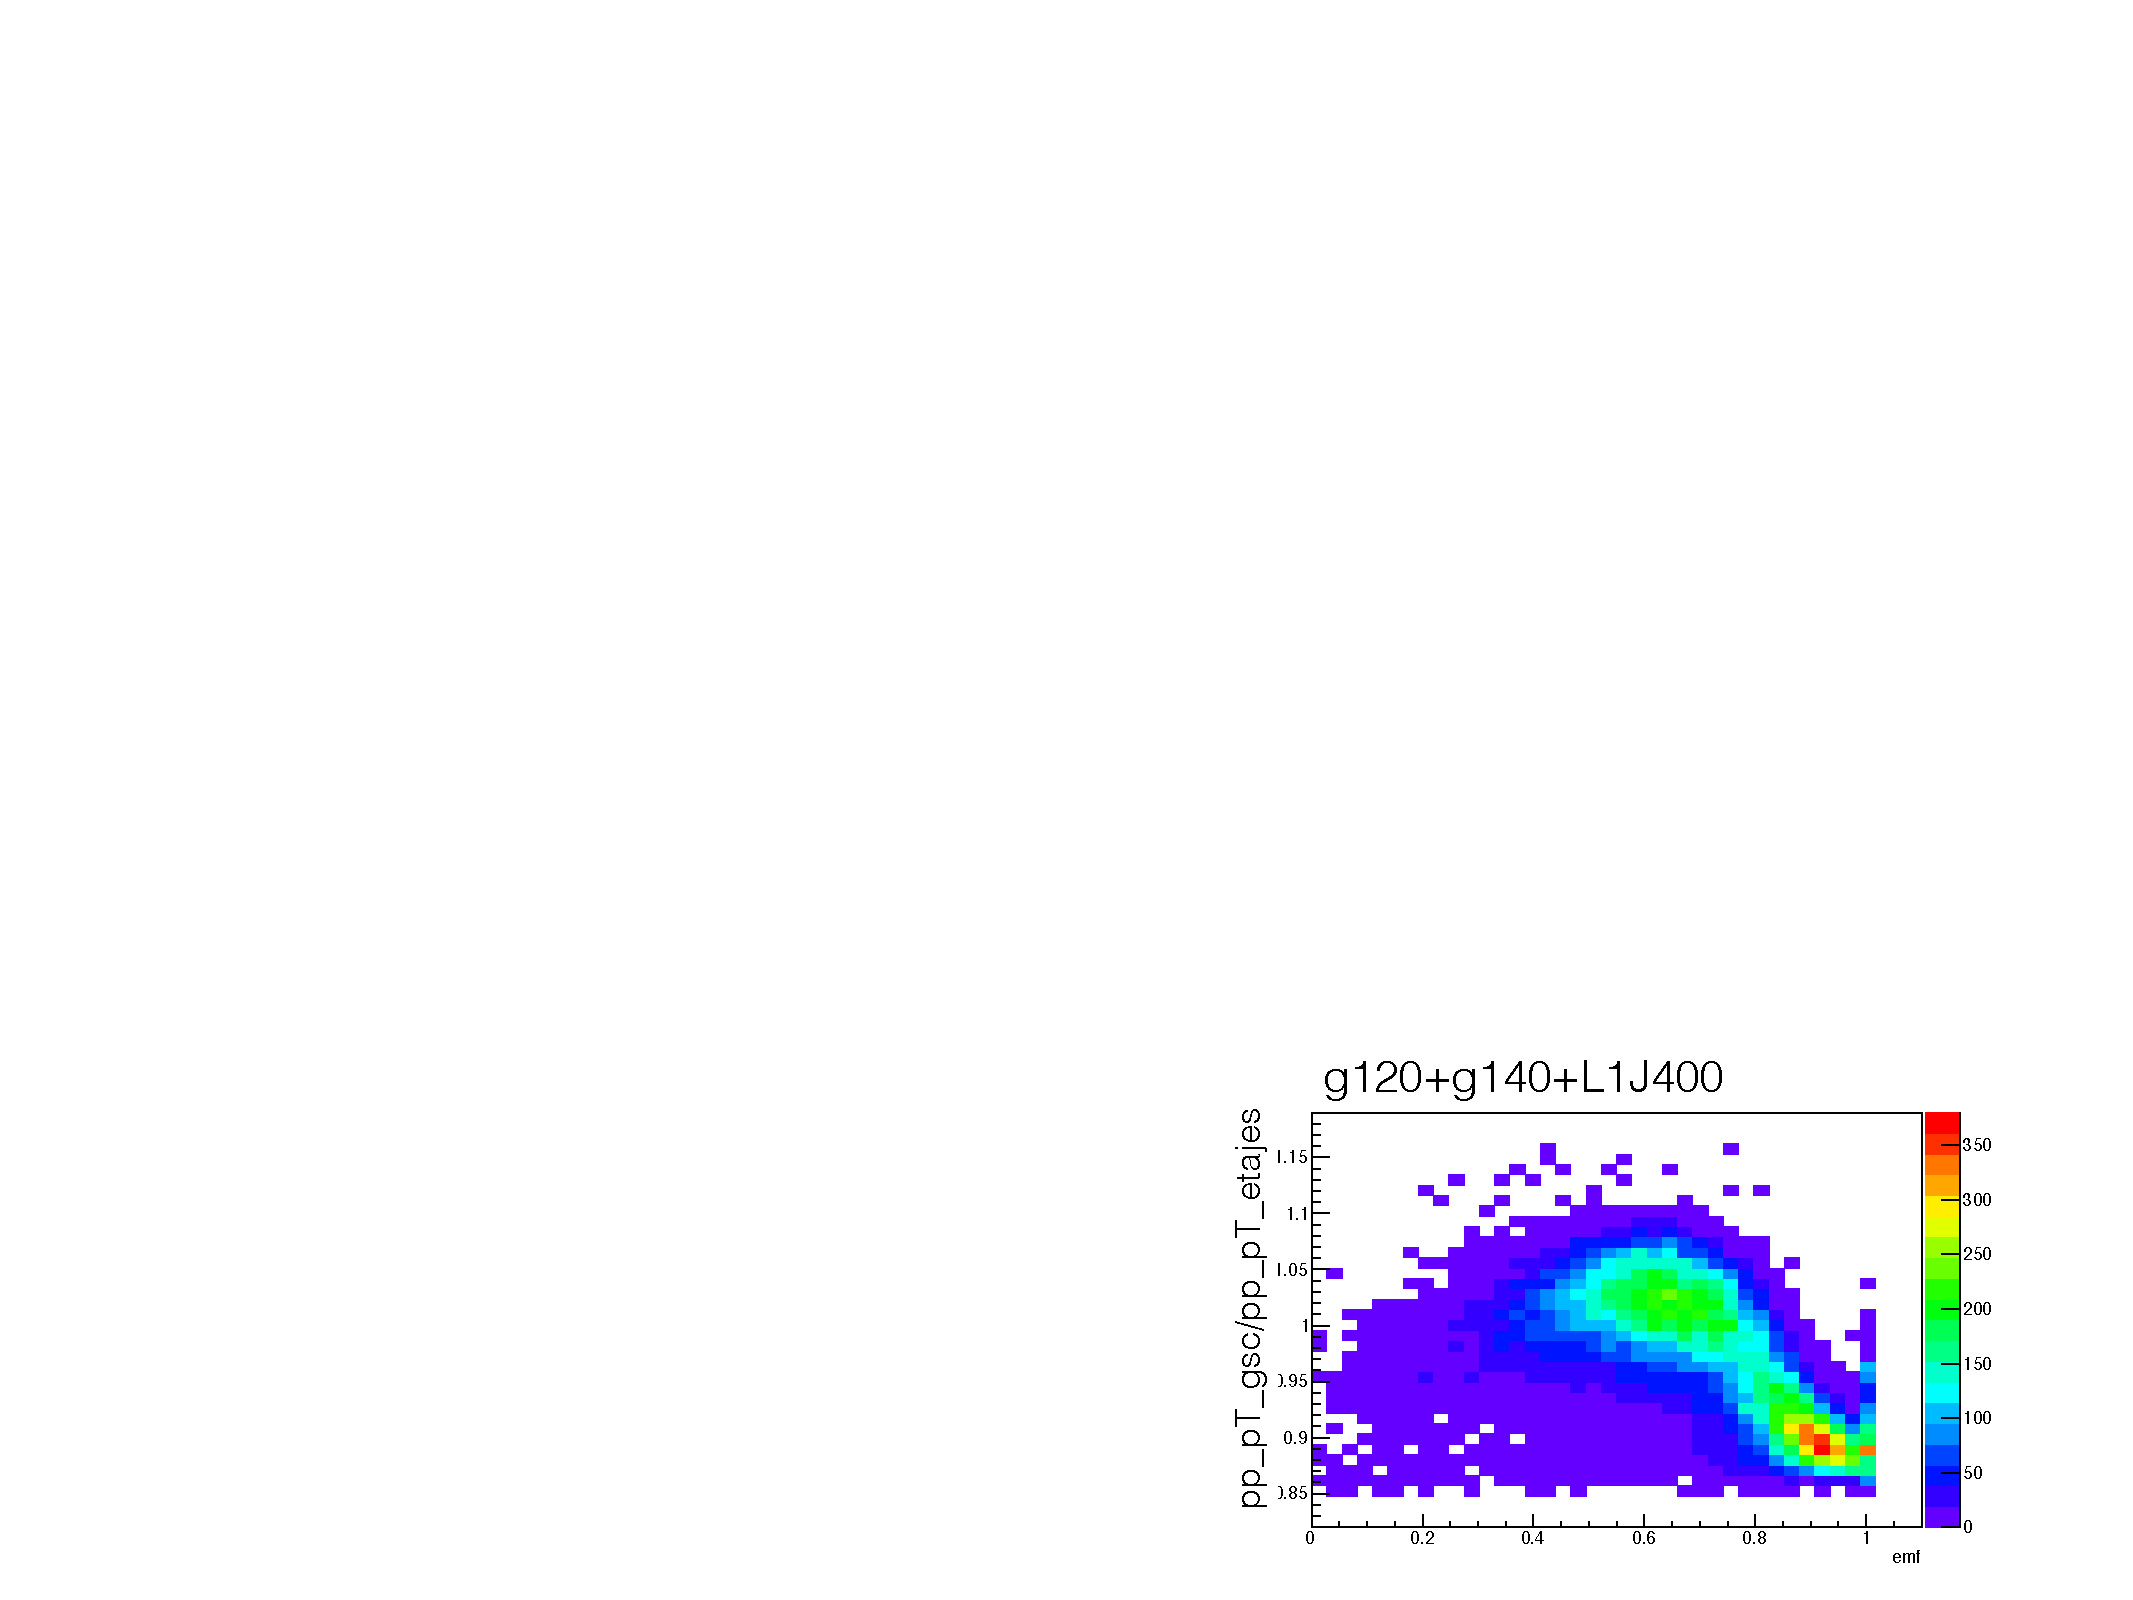
\includegraphics[width=0.5\textwidth]{figures/qualification/PhotonEx.pdf} }}%
%	\caption{The jet selection criteria in data based on different triggers. \protect\subref{a} $\pT-\eta$ phase space for different trigger regions used in the ZeroBias and express streams \protect\subref{b}The effect of the GSC calibration, as a function of the electromagnetic fraction (emf) of the jet. The peak at high emf is indicative of photons }%
%	\label{fig:TrigMap}%
%\end{figure}



\begin{figure}
\centering
\begin{subfigure}[b]{\textwidth}
    \centering
    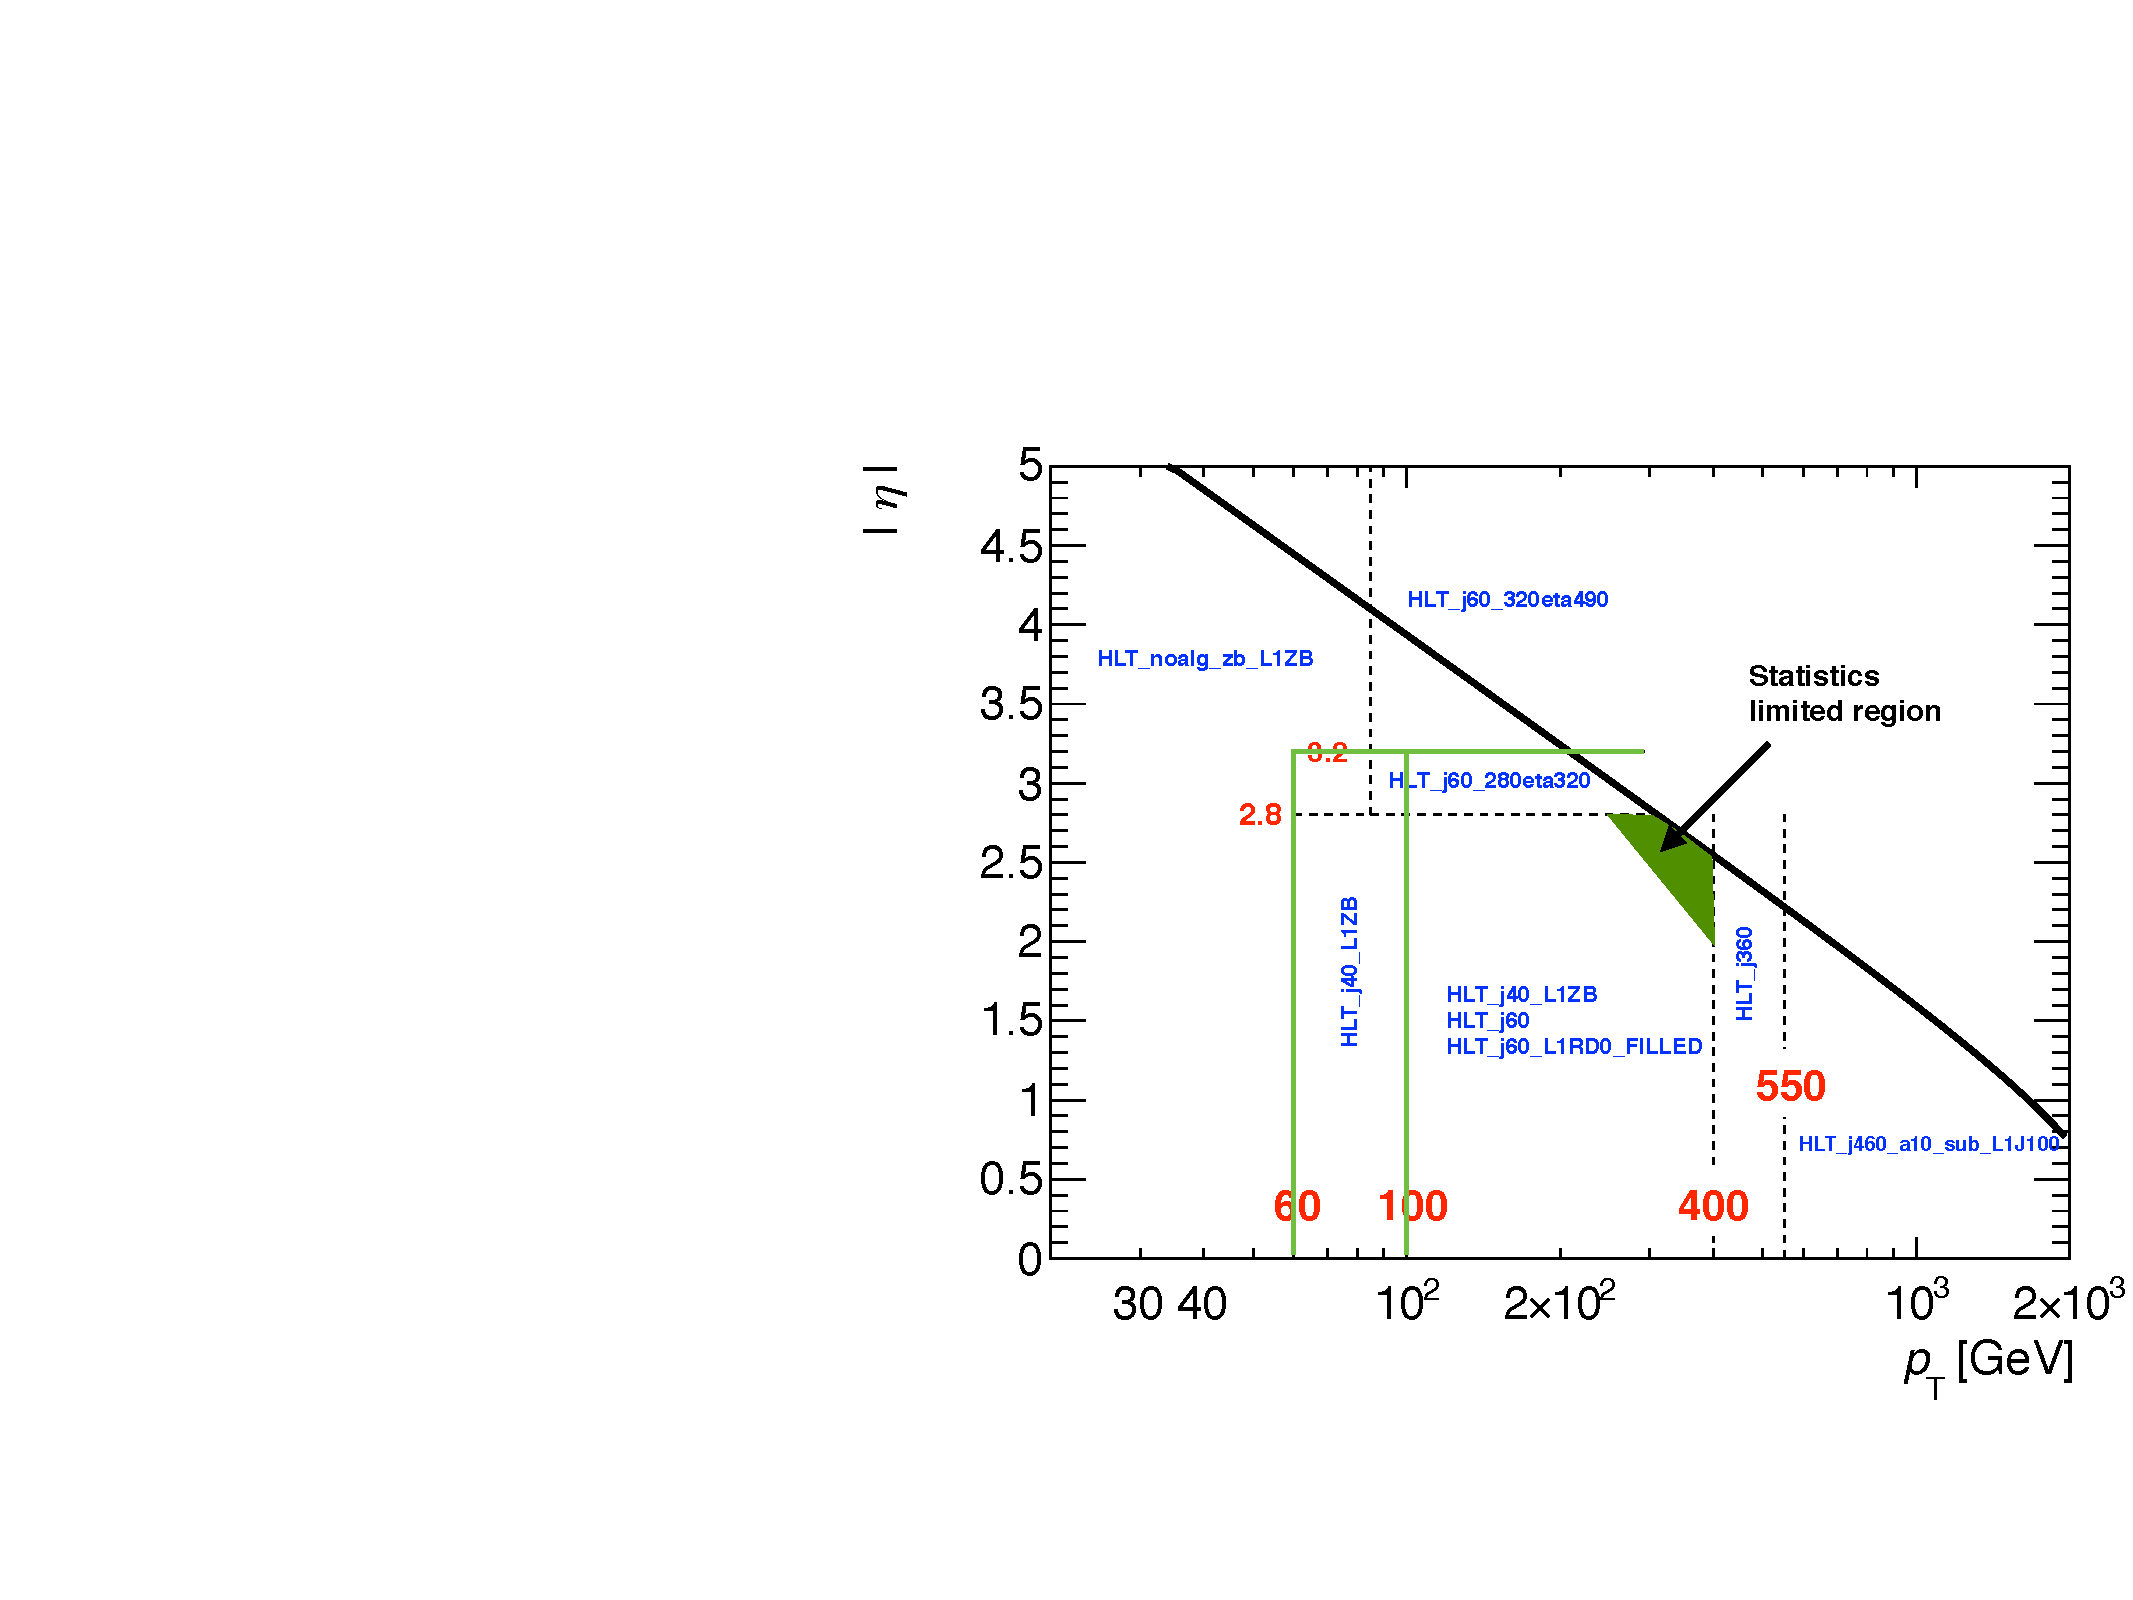
\includegraphics[width=\textwidth]{figures/qualification/TrigMap.pdf}
    \caption{}
    \label{a}
\end{subfigure} \\
\begin{subfigure}[b]{\textwidth}
    \centering
    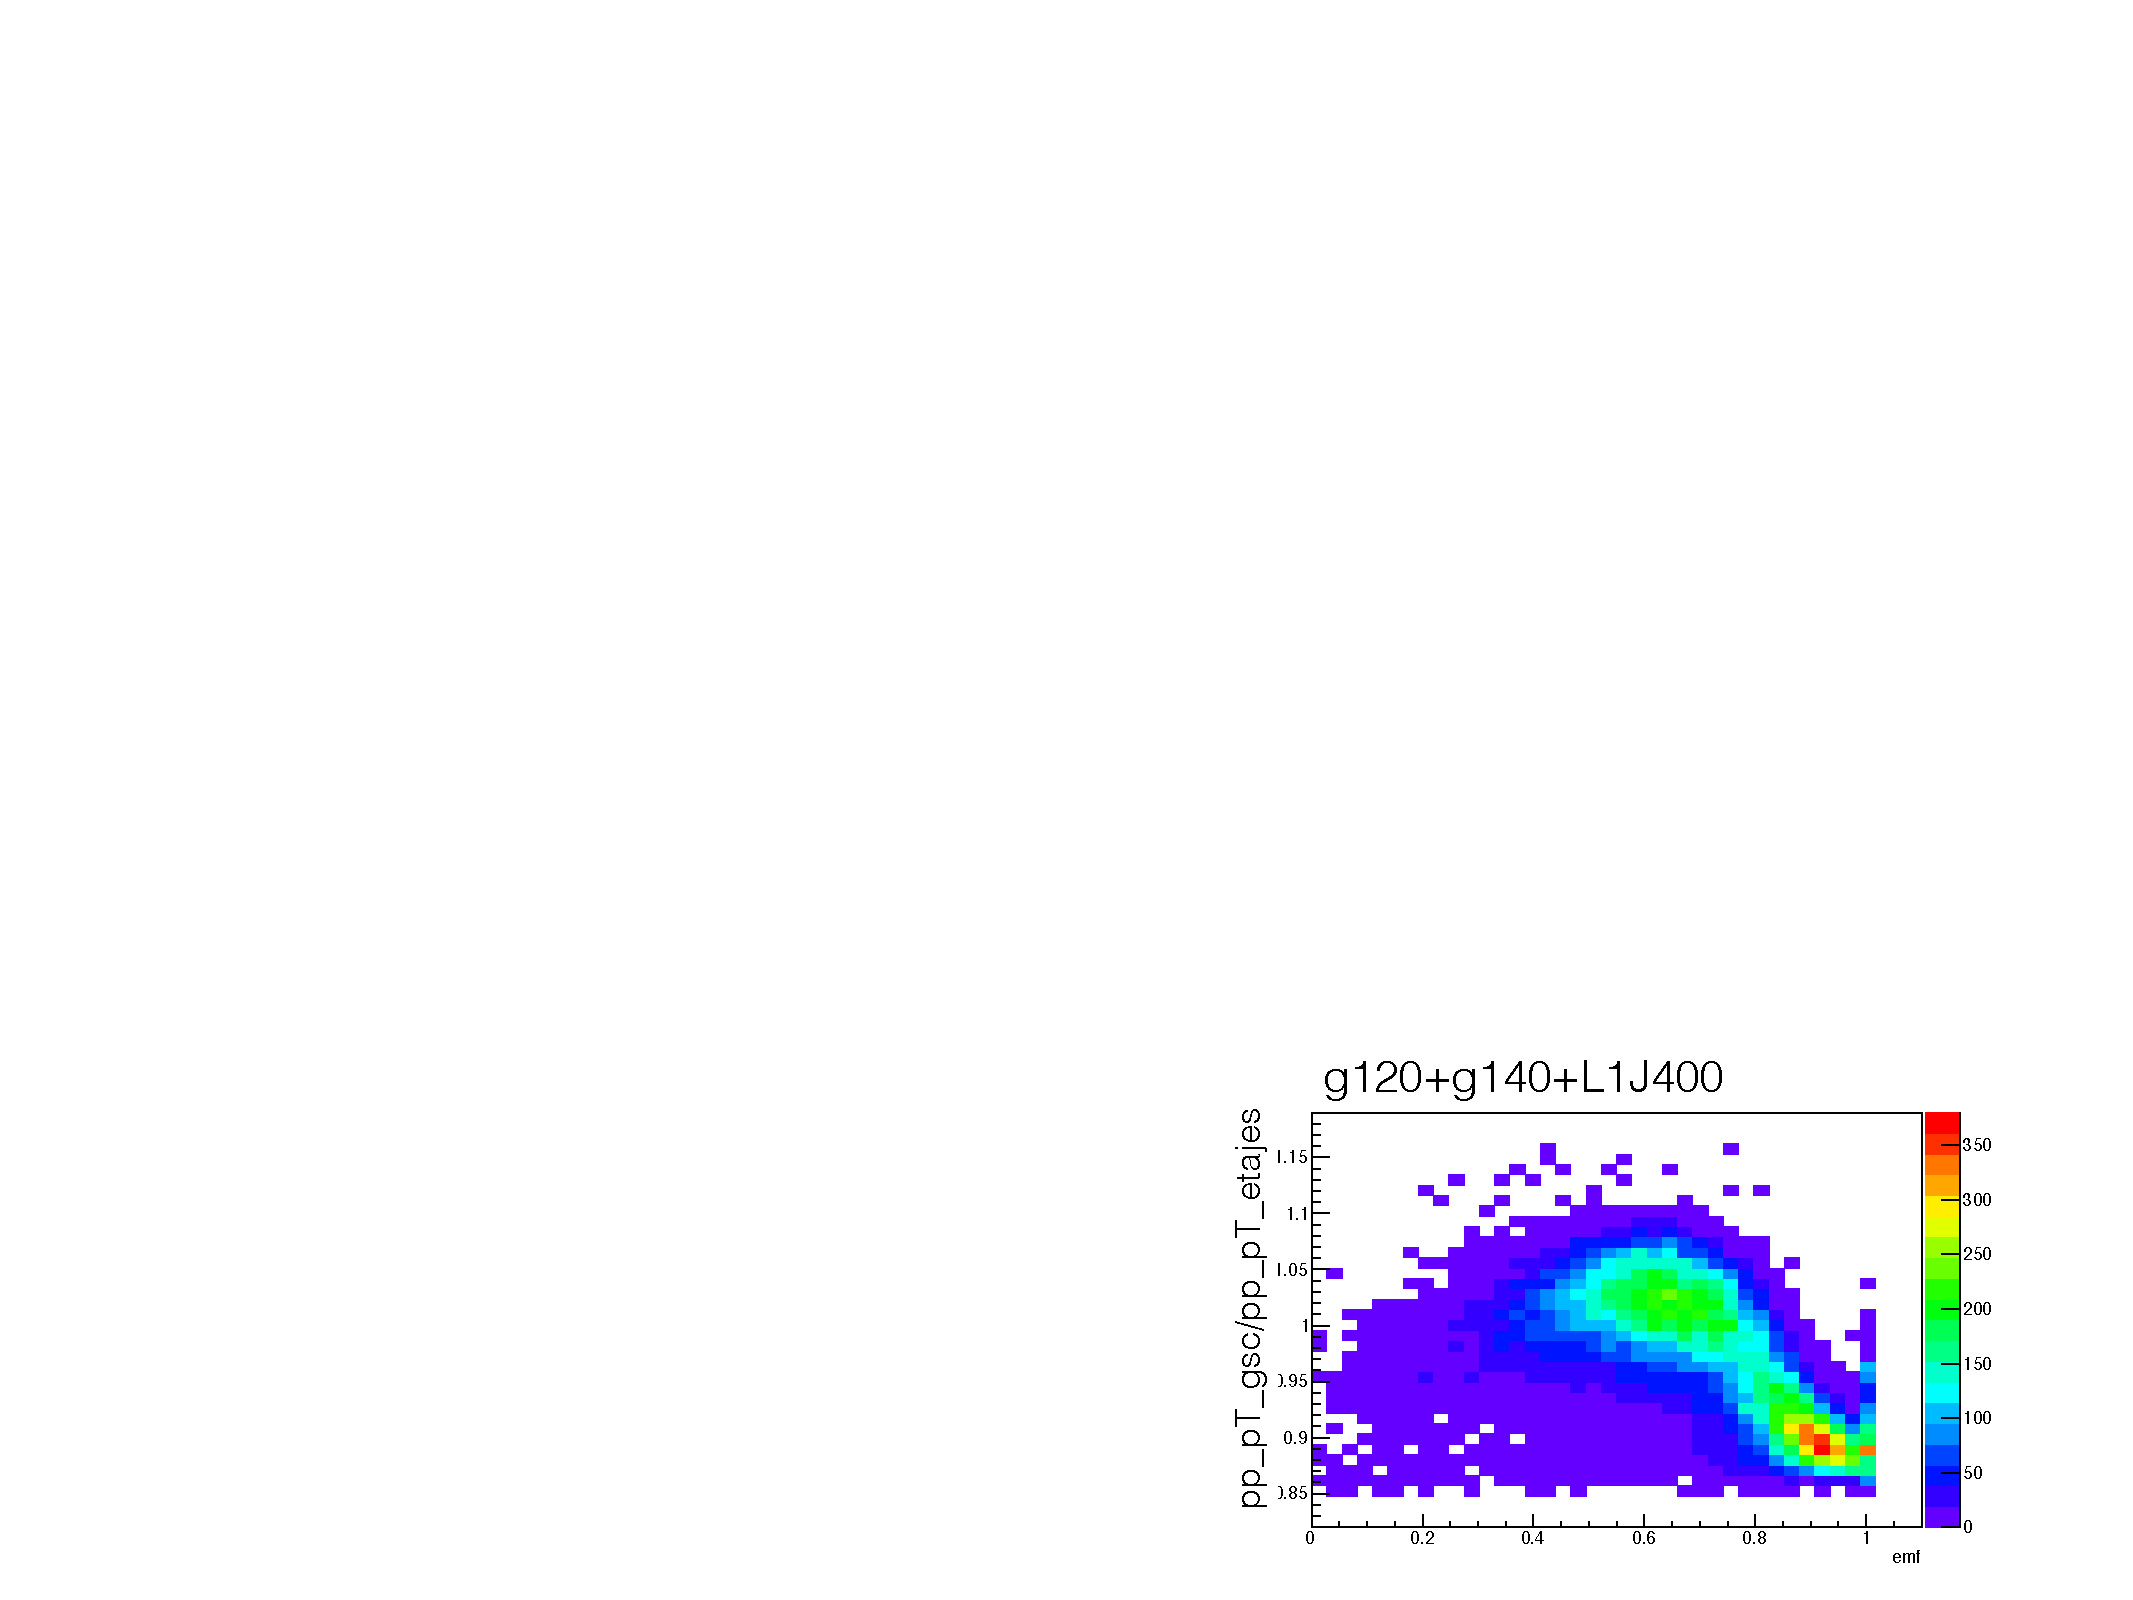
\includegraphics[width=\textwidth]{figures/qualification/PhotonEx.pdf}
    \caption{}
    \label{selection_2}
\end{subfigure}\hfill
   \caption{The jet selection criteria in data based on different triggers. \protect\subref{a} $\pT-\eta$ phase space for different trigger regions used in the ZeroBias and express streams \protect\subref{b}The effect of the GSC calibration, as a function of the electromagnetic fraction (emf) of the jet. The peak at high emf is indicative of photons }
\label{fig:TrigMap}
\end{figure}

Furthermore, events firing the HLT\_j360 trigger were vetoed if they also fired the HLT\_noalg\_L1J400, HLT\_g120\_loose, or the HLT\_g140\_loose. This was done to ensure that the jets entering the study were not in the wide turn on region of the aforementioned triggers. This also helped exclude photons (as can be seen in ~\ref{selection_2}.


MC events were filtered based on pileup. The MC generation settings included an average of combined 2015-2016 pileup profiles \cite{twiki_MC15c}. This can be seen in the top plot of Fig.~\ref{fig:mu_weight}, where the $\mu$ distribution in MC has a very wide spread, whereas the data (purely 2015) is localized around a central value. Events with $7 < \mu < 18$ were selected, and the jet $\pT$ in MC was weighted with the ratio $\mu_{\mathrm{Data}}/\mu_{\mathrm{MC}}$ (in addition to the eventweight present in JZXW MC samples).



\begin{figure}
	\centering
	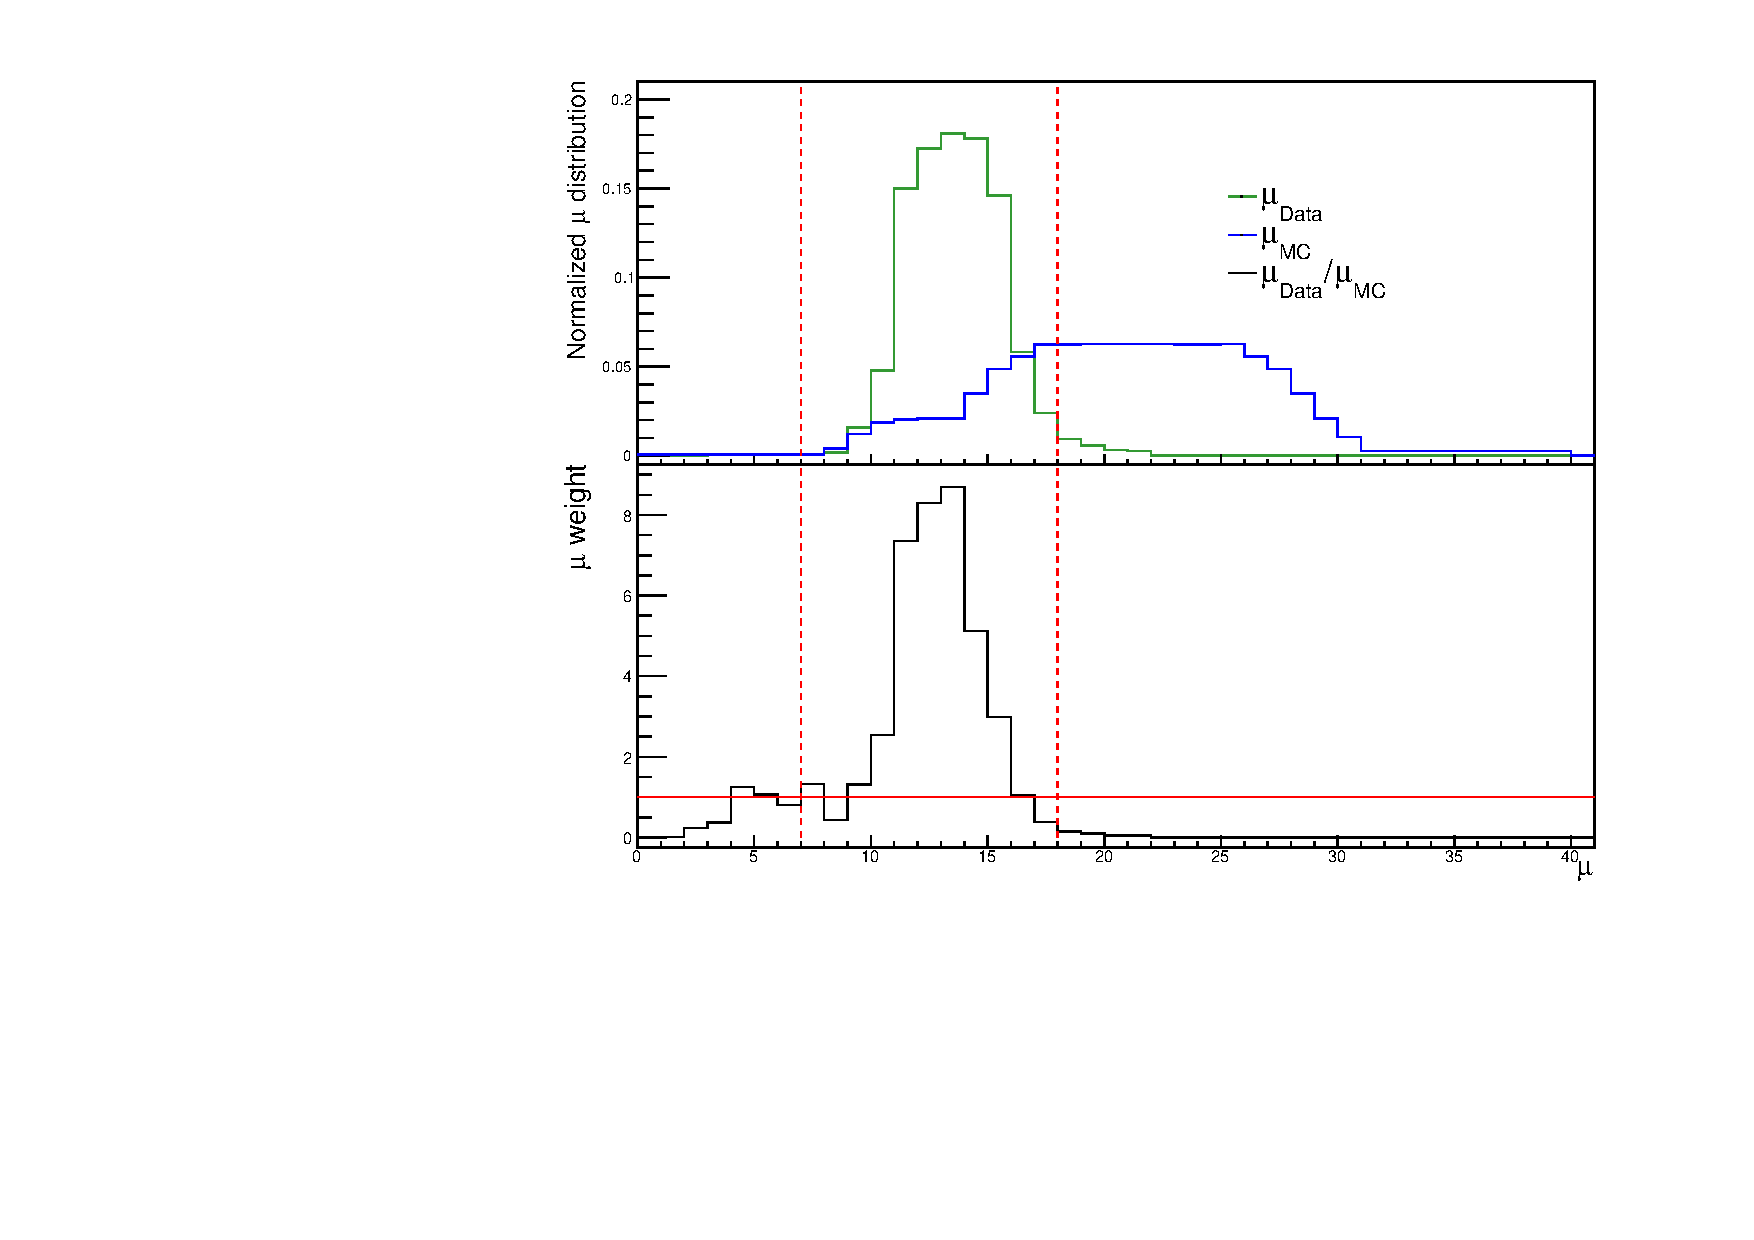
\includegraphics[width=1.0\textwidth]{figures/qualification/mu_weight.pdf}
	\caption{The top plot shows the normalized $mu$ distribution in data and MC. The bottom plot is a ratio of the two quantities. The jet selection criteria in MC is based on the pileup conditions. Events with $7 < \mu < 18$ were selected. }%
	\label{fig:mu_weight}%
\end{figure}

Other standard cuts included jet cleaning ({\it{LooseBad}} cut level with the option {\it{doUgly}} set to {\it TRUE}) and applying a GRL data15\_13TeV.periodAllYear\_DetStatus-v75-repro20-01\_DQDefects-00-02-02\_PHYS\_Standard\\GRL\_All\_Good\_25ns.xml)

The HI, EMTopo, and Truth jets were also isolated and matched to each other (and to truth in MC) with the criteria given in Tables~\ref{table:iso_criteria} and \ref{table:match_criteria}. The isolation \pt\ cut choice was dictated by the minimum\ \pT \ with which the HI and EMTopo jets are reconstructed (5 GeV for HI, 10 GeV for EMTopo). An investigation showed that for isolation $\pT$ cuts below 20 GeV, there was a large difference (upto at least a factor of ~2) in the number of EMTopo jets matched to truth jets, compared to HI jets matched to truth jets. The cross calibration factors were evaluated for jets with $30 < \pT < 1000 $ GeV.

\begin{table}[ht]
\caption{Isolation criteria used in the evaluation of the nominal cross calibration factors}
\centering
\begin{tabular}{c c c}
\hline\hline
Jet Collection & Radius cut & $\pT$ cut [GeV] \\ [0.5ex] % inserts table %heading
\hline
AntiKt4EMTopo & 1.0 & 20.0 \\ 
AntiKt4HI & 1.0 & 20.0 \\ 
Truth (in MC) & 0.6 & 20.0 \\ 
\hline
\end{tabular}
\label{table:iso_criteria}
\end{table}

\begin{table}[ht]
\caption{Matching criteria used in the evaluation of the nominal cross calibration factors}
\centering
\begin{tabular}{c c}
\hline\hline
Jet Collections & Radius cut \\ [0.5ex] % inserts table %heading
\hline
AntiKt4EMTopo + Truth & 0.2 \\ 
AntiKt4HI + Truth & 0.3 \\ 
AntiKt4(EMTopo+HI) & 0.4\\ 
\hline
\end{tabular}
\label{table:match_criteria}
\end{table}


%-------------------------------------------------------------------------------
\section{Procedure}
\label{sec:qual_procedure}
%-------------------------------------------------------------------------------

The results presented here were performed using the ATLAS detector and calorimeter systems ~\cite{Aad:2008zzm}. Jets with a radius of $R=0.4$ were reconstructed using the \\antikt \ algorithm.  The specifics of this procedure as applied to reconstruct the standard EMTopo jets and the HI jets are described in detail in \cite{Aad:2011he} and \cite{Aad:hi_jets} respectively. A brief summary is given below.

The EMTopo jets reconstruction involves using topological clusters of energy deposits in the calorimeter (calorimeter description in ~\cite{Aad:2008zzm}). The \\antikt \ algorithm \cite{antikt_algo}, as implemented in the FastJet sofware package \cite{fastjet_algo} is applied to these clusters, to reconstruct EMTopo jets with a $R = 0.4$.  The background in these jets, coming from the pile-up, is reduced by applying a $\pT$ and jet area dependent subtraction \cite{pp_pileup_subtr}. The jets are then calibrated using a energy and $\eta$ dependent calibration factor, derived from MC studies. The EMTopo jets for this study were calibrated up to MC based EtaJES, as described in \cite{CalibReco}.

The HI jet reconstruction also uses the anti-$k_{T}$ algorithm, but the inputs are $\Deta \times \Dphi = 0.1 \times \frac{\pi}{32}$ logical towers, deriving from the energy deposited in calorimeter cells. A fundamental difference between the reconstruction algorithms is how the underlying event (UE) is dealt with. The UE subtraction procedure involves the UE average tranvserse energy density ($\rho$), and the magnitude ($\nu_{2}$) and phase ($\Psi_{2}$) of the elliptic modulation from to flow. The subtraction applied to each cell within the jet is given as: 
\begin{align}
\Et^{\mathrm{subtr}} = \Et^{\mathrm{cell}} - \rho(\eta^{\mathrm{cell}},\phi^{\mathrm{cell}})A^{\mathrm{cell}} \{1 + 2\nu_{2 i}\cos[2(\phi - \Psi_2)]\}
\end{align}
where $\eta^{\mathrm{cell}}$ and $\phi^{\mathrm{cell}}$ are the cell coordinates, and $A^{\mathrm{cell}}$ is the cell area in $\eta-\phi$ space. $\Et^{\mathrm{subtr}}$ and $ \Et^{\mathrm{cell}}$ are the cell energies before and after subtraction \cite{HIjesnote}. The average UE transverse energy density is estimated from the cell transverse energies, whereas $\Psi_2$ is the determined from the FCal.
\begin{align}
\rho &\equiv \left\langle \frac{\Et^{\mathrm{cell}}}{A^{\mathrm{cell}}}\right\rangle \\
\Psi_2 &= \frac{1}{2} \tan^{-1}\frac{\sum \Et^{\mathrm{cell}} \sin 2\phi^{\mathrm{cell}} }{\sum \Et^{\mathrm{cell}} \cos 2\phi^{\mathrm{cell}} } \\
\nu_2 &= \frac{\sum \Et^{\mathrm{cell}} \cos 2(\phi^{\mathrm{cell}} - \Psi_2) }{\sum \Et^{\mathrm{cell}}}
\end{align}

The subtracted energy is seen to be independent of the jet\ \Et \ 

%IMPORTANT ----- insert subtracted pt figure here  ----- IMPORTANT


A summary of the differences between the EMTopo and HI jet reconstruction methods is given in Table \ref{table:algo_diff}.
\begin{table}[h]
\centering
\caption{A summary of the differences between the EMTopo and HI jet reconstruction algorithm. Adapted from \cite{HIjesnote}.}
\begin{tabular}{|c|c|c|}
\hline
            & EMTopo                 & HI                           \\ \hline
Inputs      & Topological clusters   & Calorimeter towers           \\ \hline
Subtraction & Median $\pT$ density & Average local energy density \\ \hline
\end{tabular}
\label{table:algo_diff}
\end{table}




The heavy ion jets were calibrated (upto {\it EtaJES}) using the procedure given in \cite{HICalib}, and the EMTopo jets were calibrated upto GSC (i.e. {\it JetArea\_Residual\_Origin\_EtaJES\_GSC}) using the ICHEP recommendations \cite{CalibReco}. This was done so that the cross calibration factors could be applied as a correction on top of the insitu correction. This allowed changing the insitu correction, without re-deriving the cross-calibration factors. 

A ratio of the EMTopo and HI jets, selected as described in Section~\ref{sec:datasets} was taken in both data and MC. The relative response and resolution in data and MC is shown in Fig.~\ref{fig:data_rel_resp} and \ref{fig:mc_rel_resp}. The distributions were calculated in the following $|\eta|$ bins: 0 - 0.3, 0.3 - 0.8, 0.8 - 1.2, 1.2 - 2.1, 2.1 - 2.8, 2.8 - 3.6, 3.6 - 4.4.

\begin{figure}[h]
\centerline{
         \begin{tabular}{cc}
            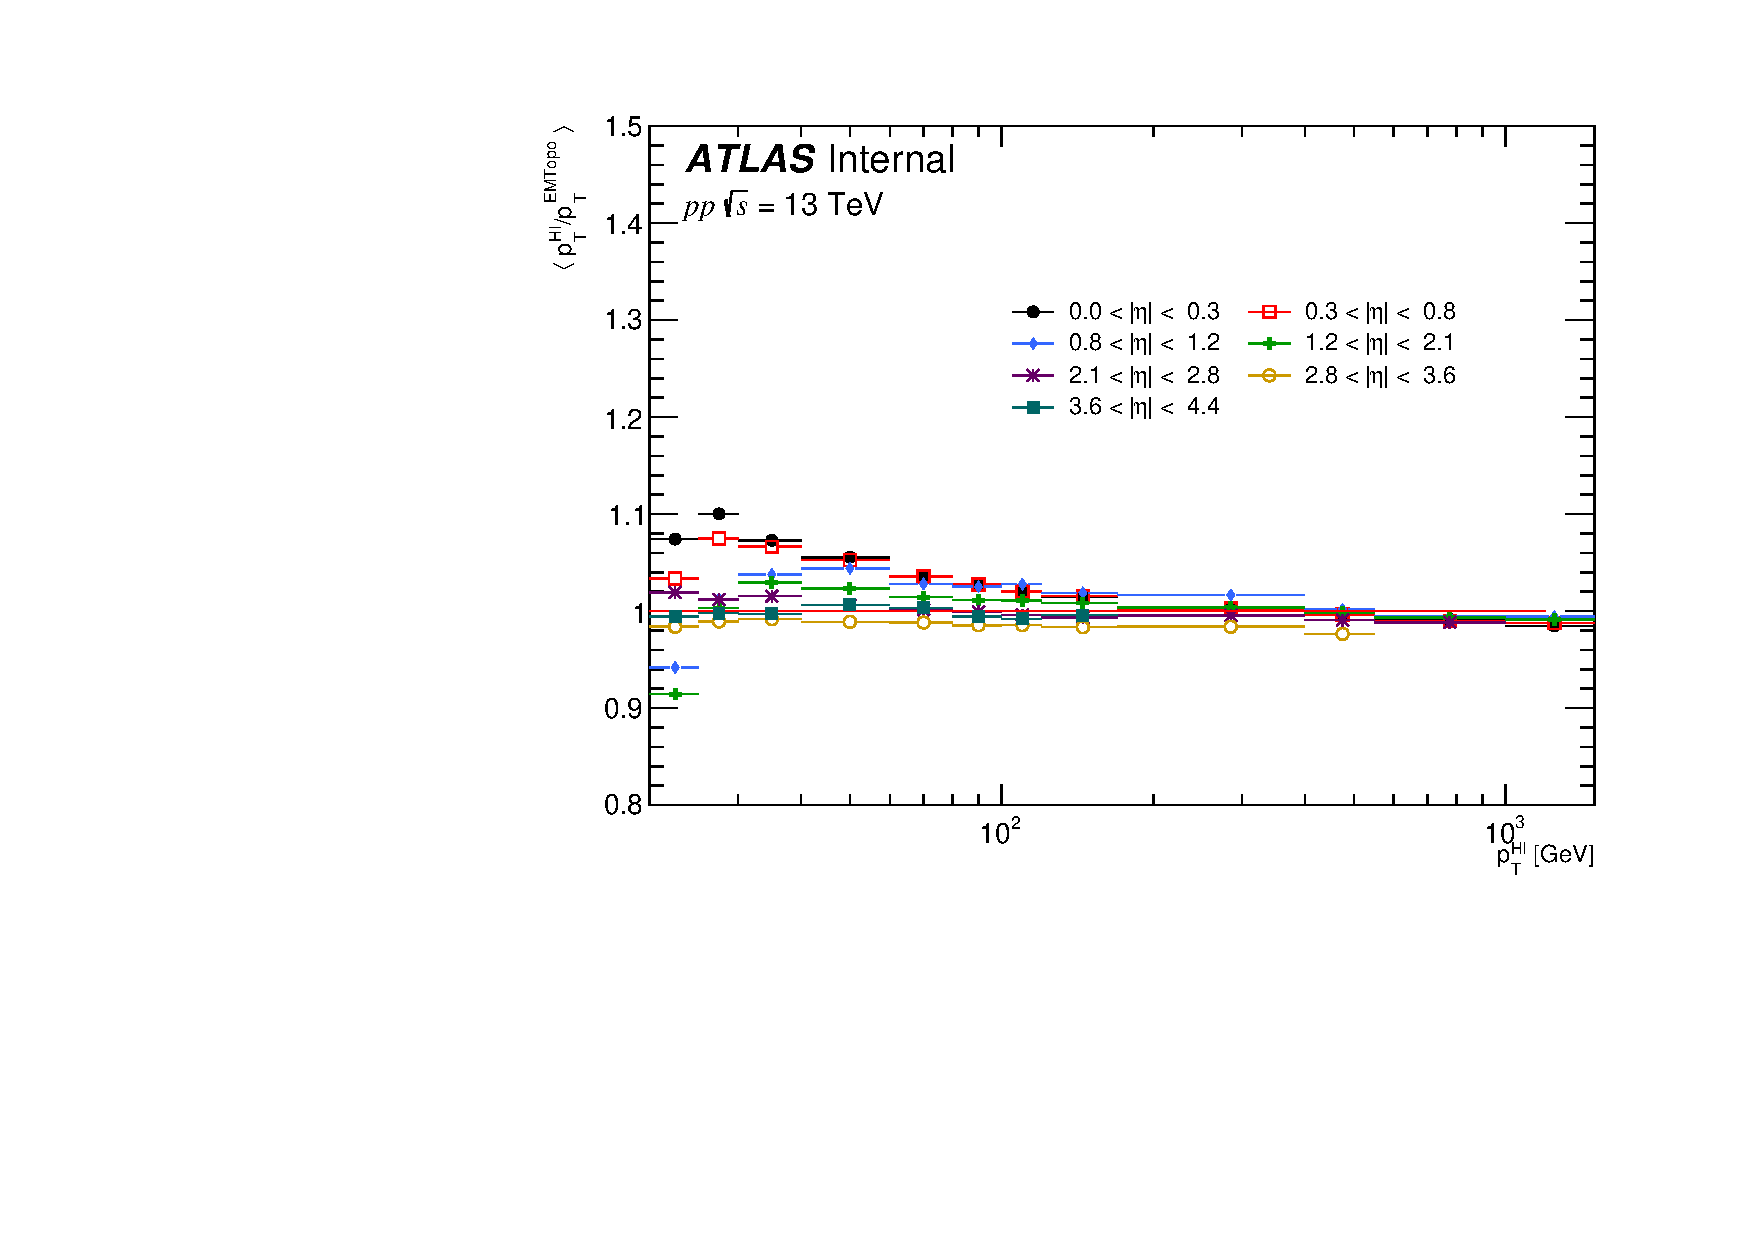
\includegraphics[width=0.5\textwidth]{figures/qualification/data_combined_h_resp12.pdf} & 
            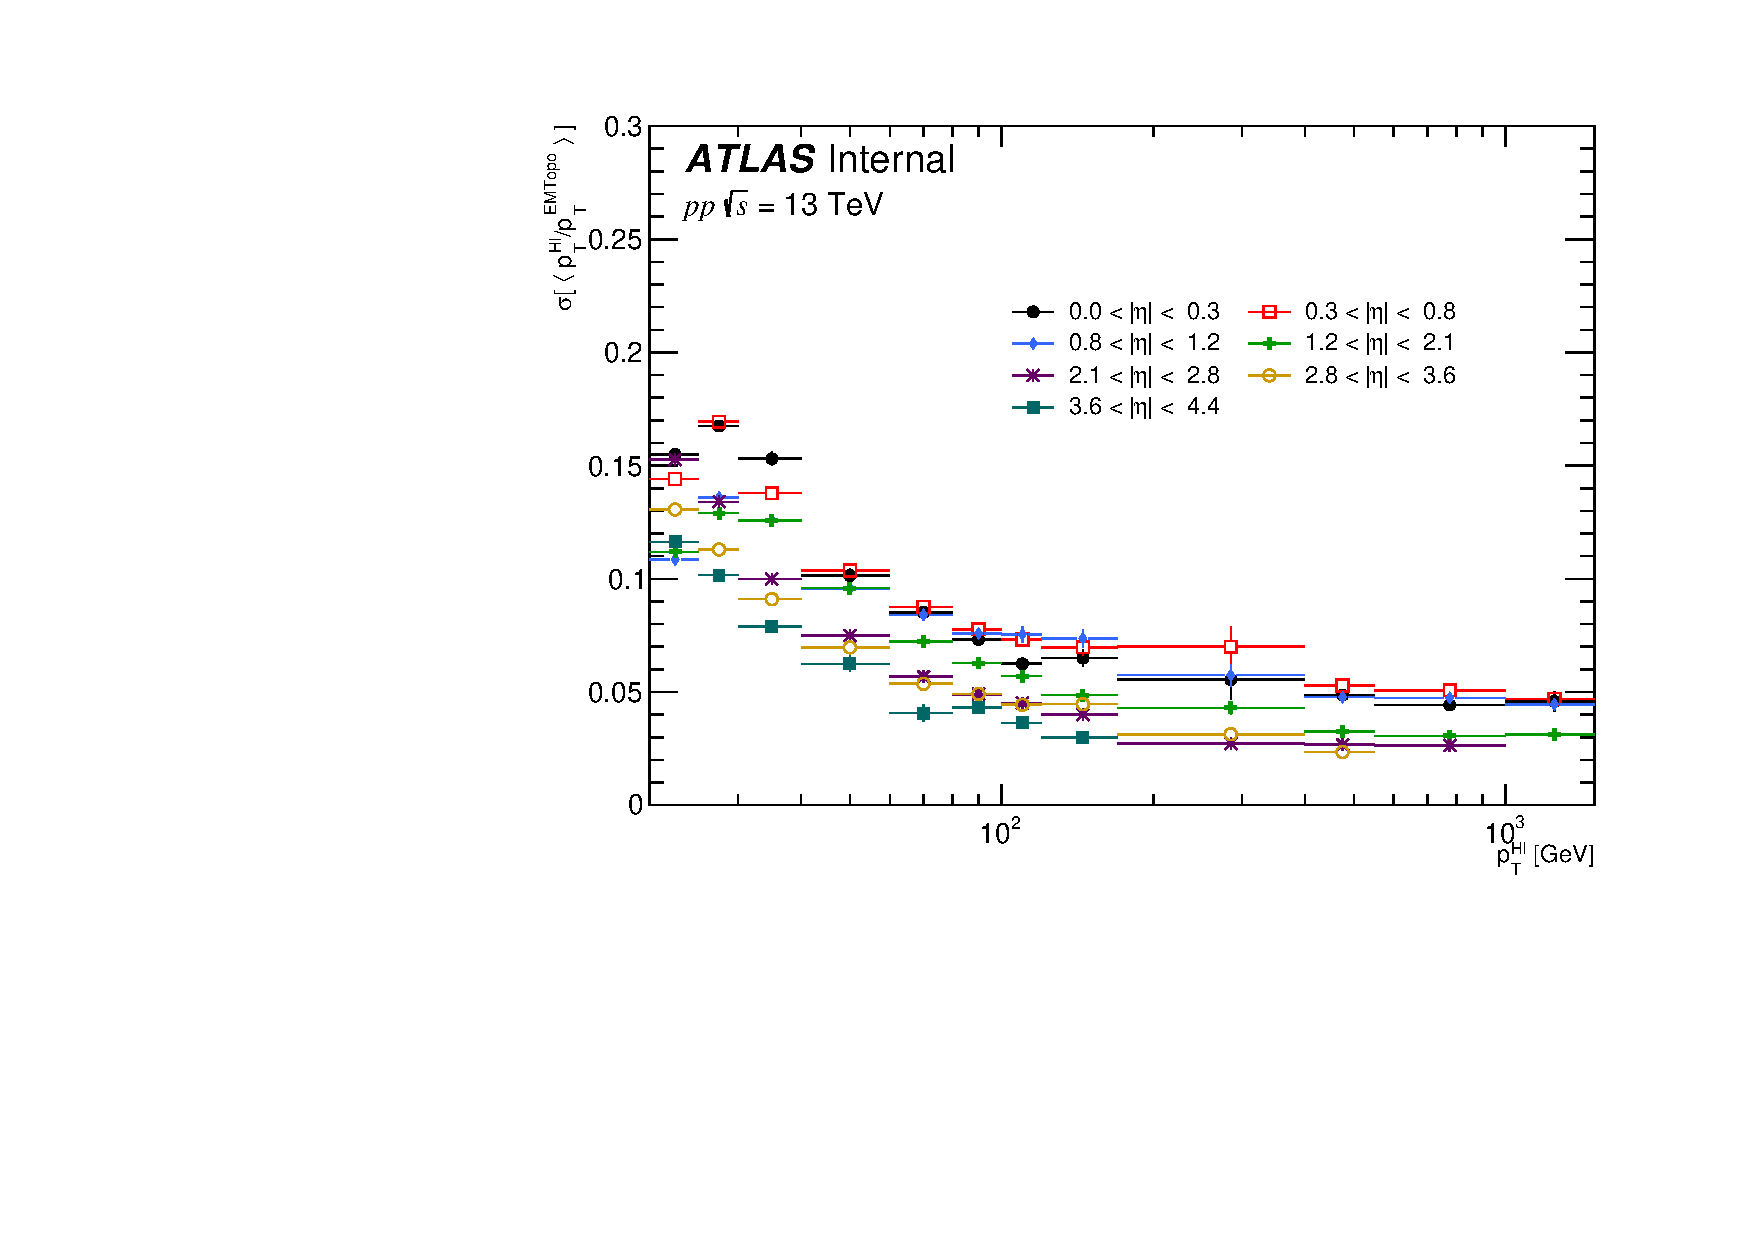
\includegraphics[width=0.5\textwidth]{figures/qualification/data_combined_h_resp12_jer.pdf} \\
      \end{tabular}
      }
\caption{The relative response (left) and relative resolution (right) in data, as a function of the HI jet $\pT$}
\label{fig:data_rel_resp}
\end{figure}

\begin{figure}[h]
\centerline{
         \begin{tabular}{cc}
            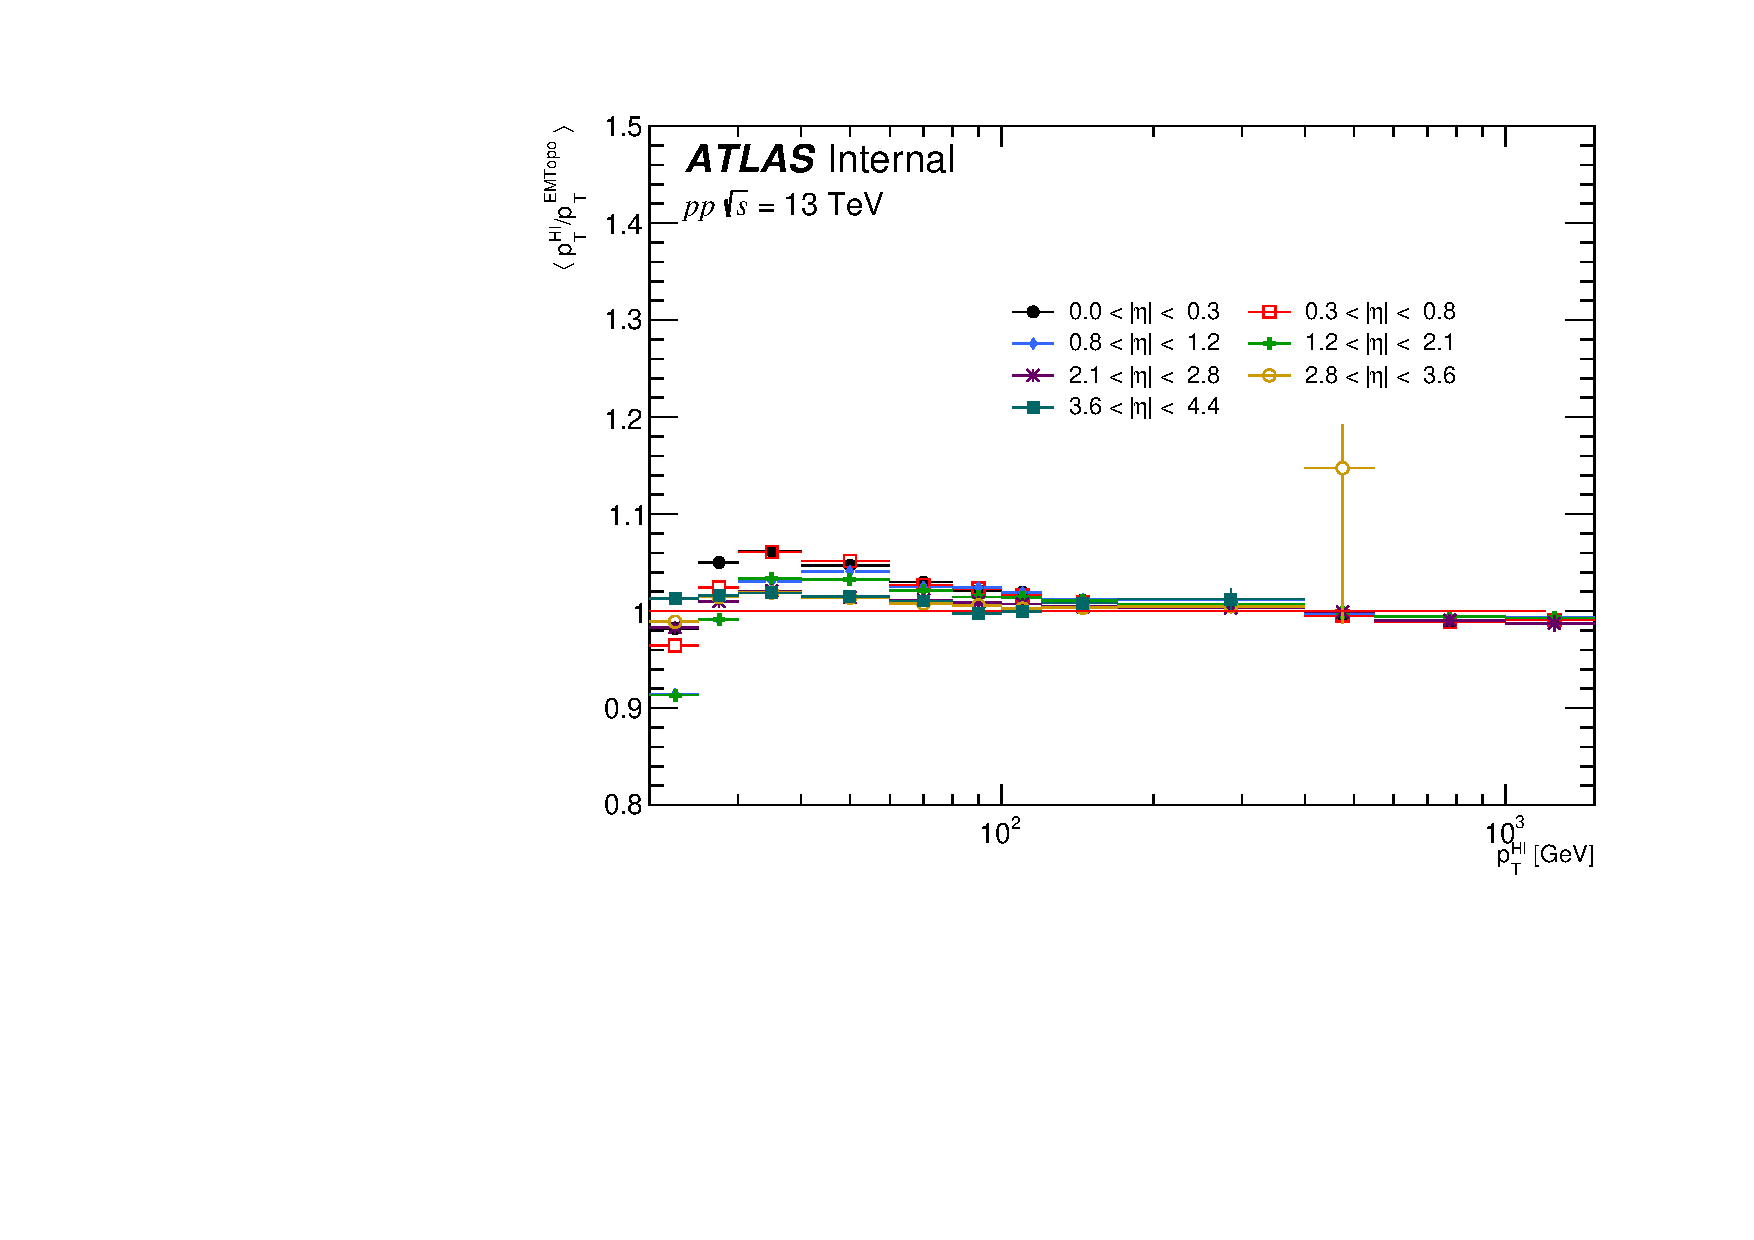
\includegraphics[width=0.5\textwidth]{figures/qualification/mc_combined_h_resp12.pdf} & 
            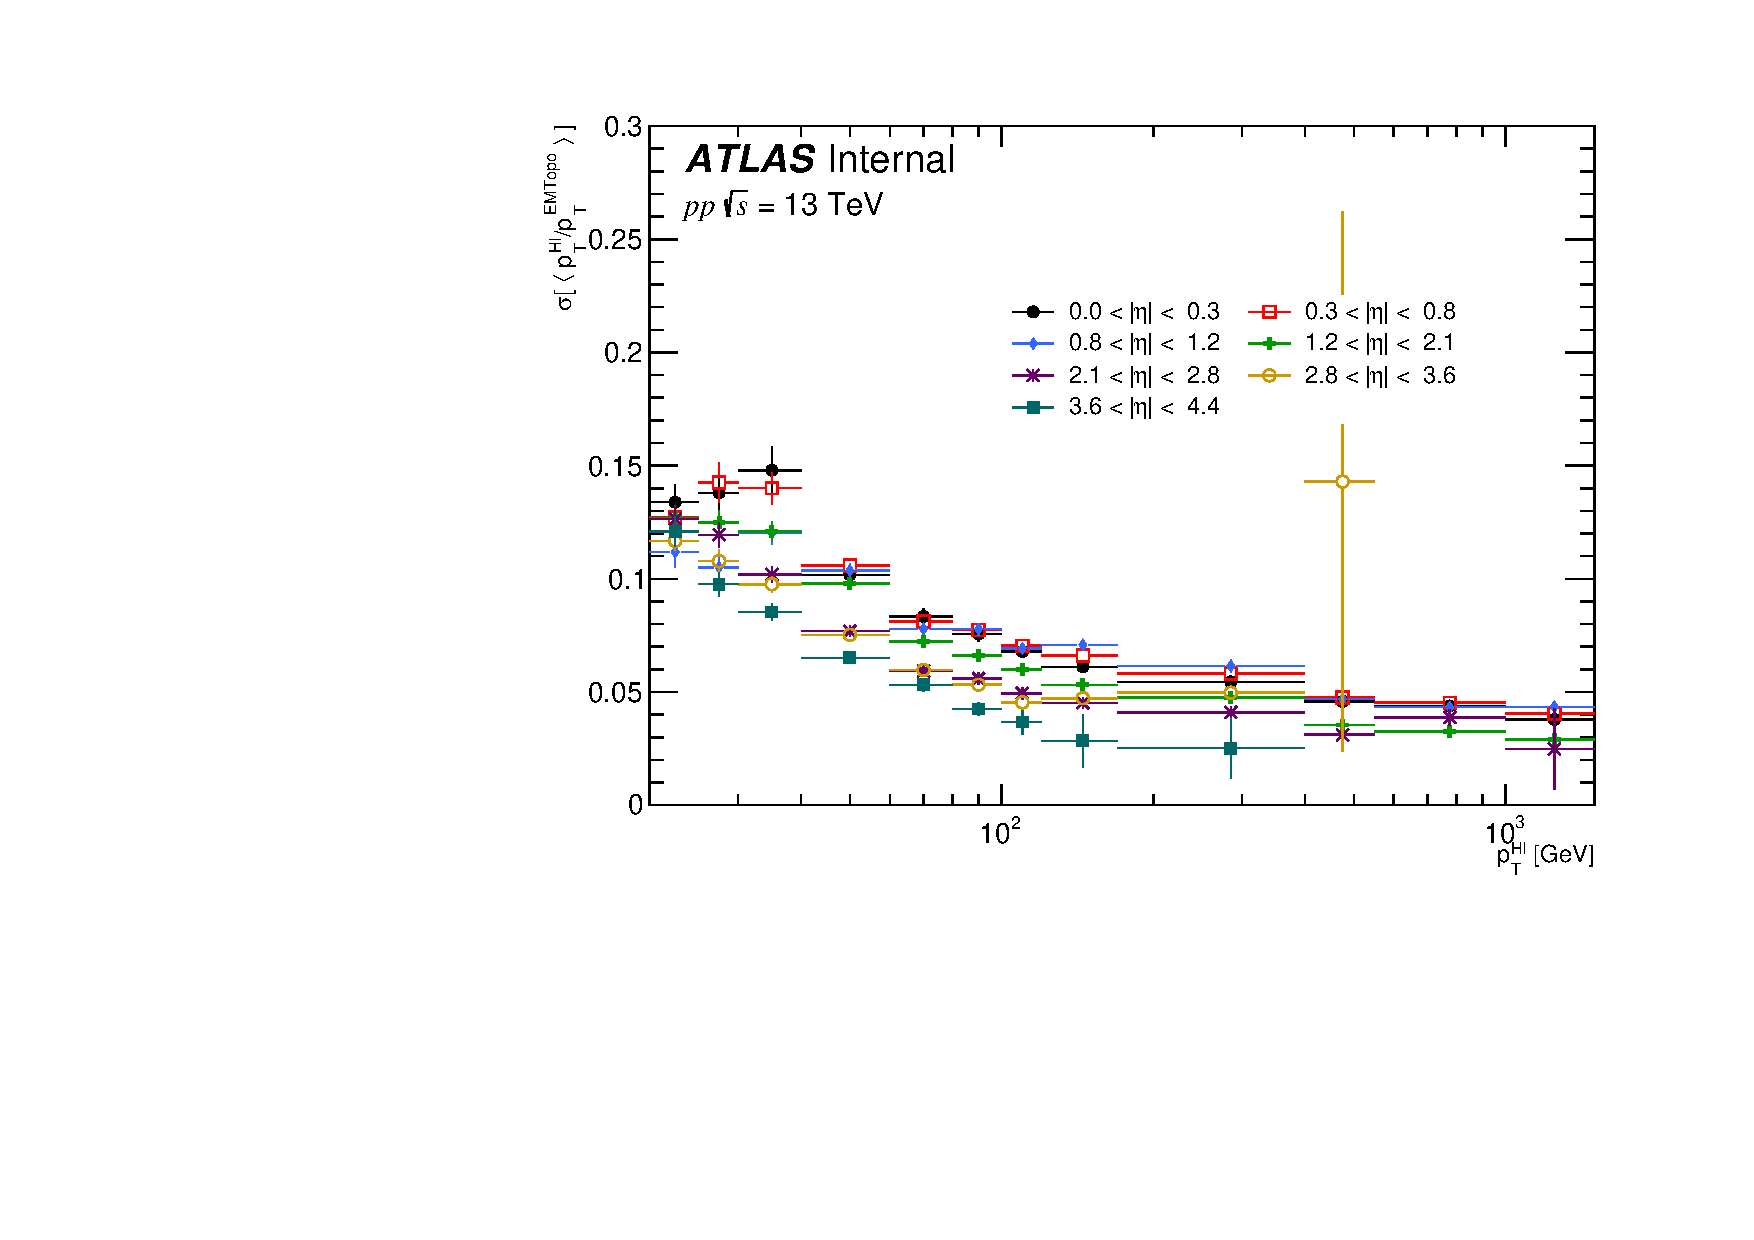
\includegraphics[width=0.5\textwidth]{figures/qualification/mc_combined_h_resp12_jer.pdf} \\
      \end{tabular}
      }
\caption{The relative response (left) and relative resolution (right) in MC, as a function of the HI jet $\pT$}
\label{fig:mc_rel_resp}
\end{figure}


The cross calibration factors, obtained by taking a ratio of the above relative response plots, were fit to a polynomial in log [$c_0 + c_1 \log(x) + c_2( \log(x))^2$] and are shown in Fig.~\ref{fig:cc_factors}. A ratio of the data to the fits is shown in Fig.~\ref{subfig:data2fit}.


\begin{figure}[h]
\centerline{
         \begin{tabular}{cc}
            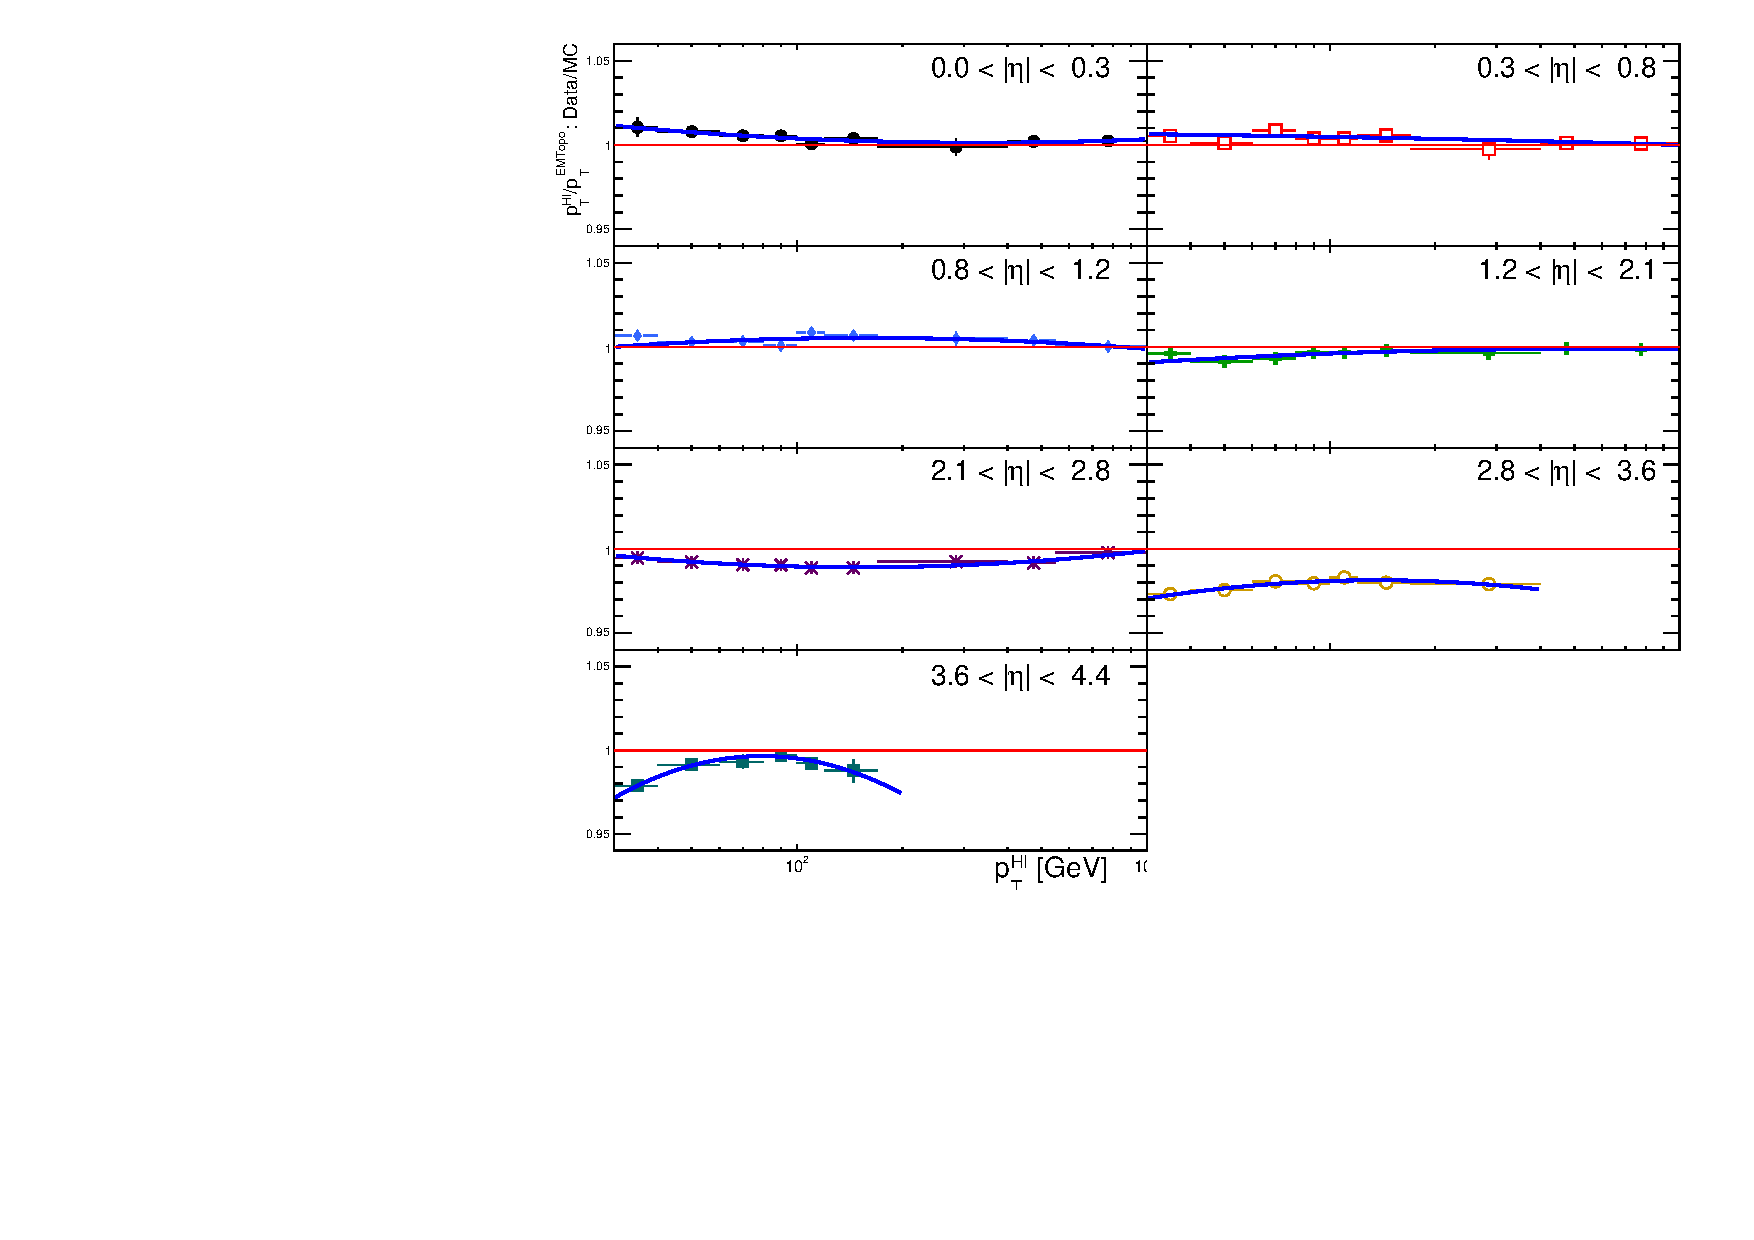
\includegraphics[width=0.5\textwidth]{figures/qualification/factors_w_fits} & 
            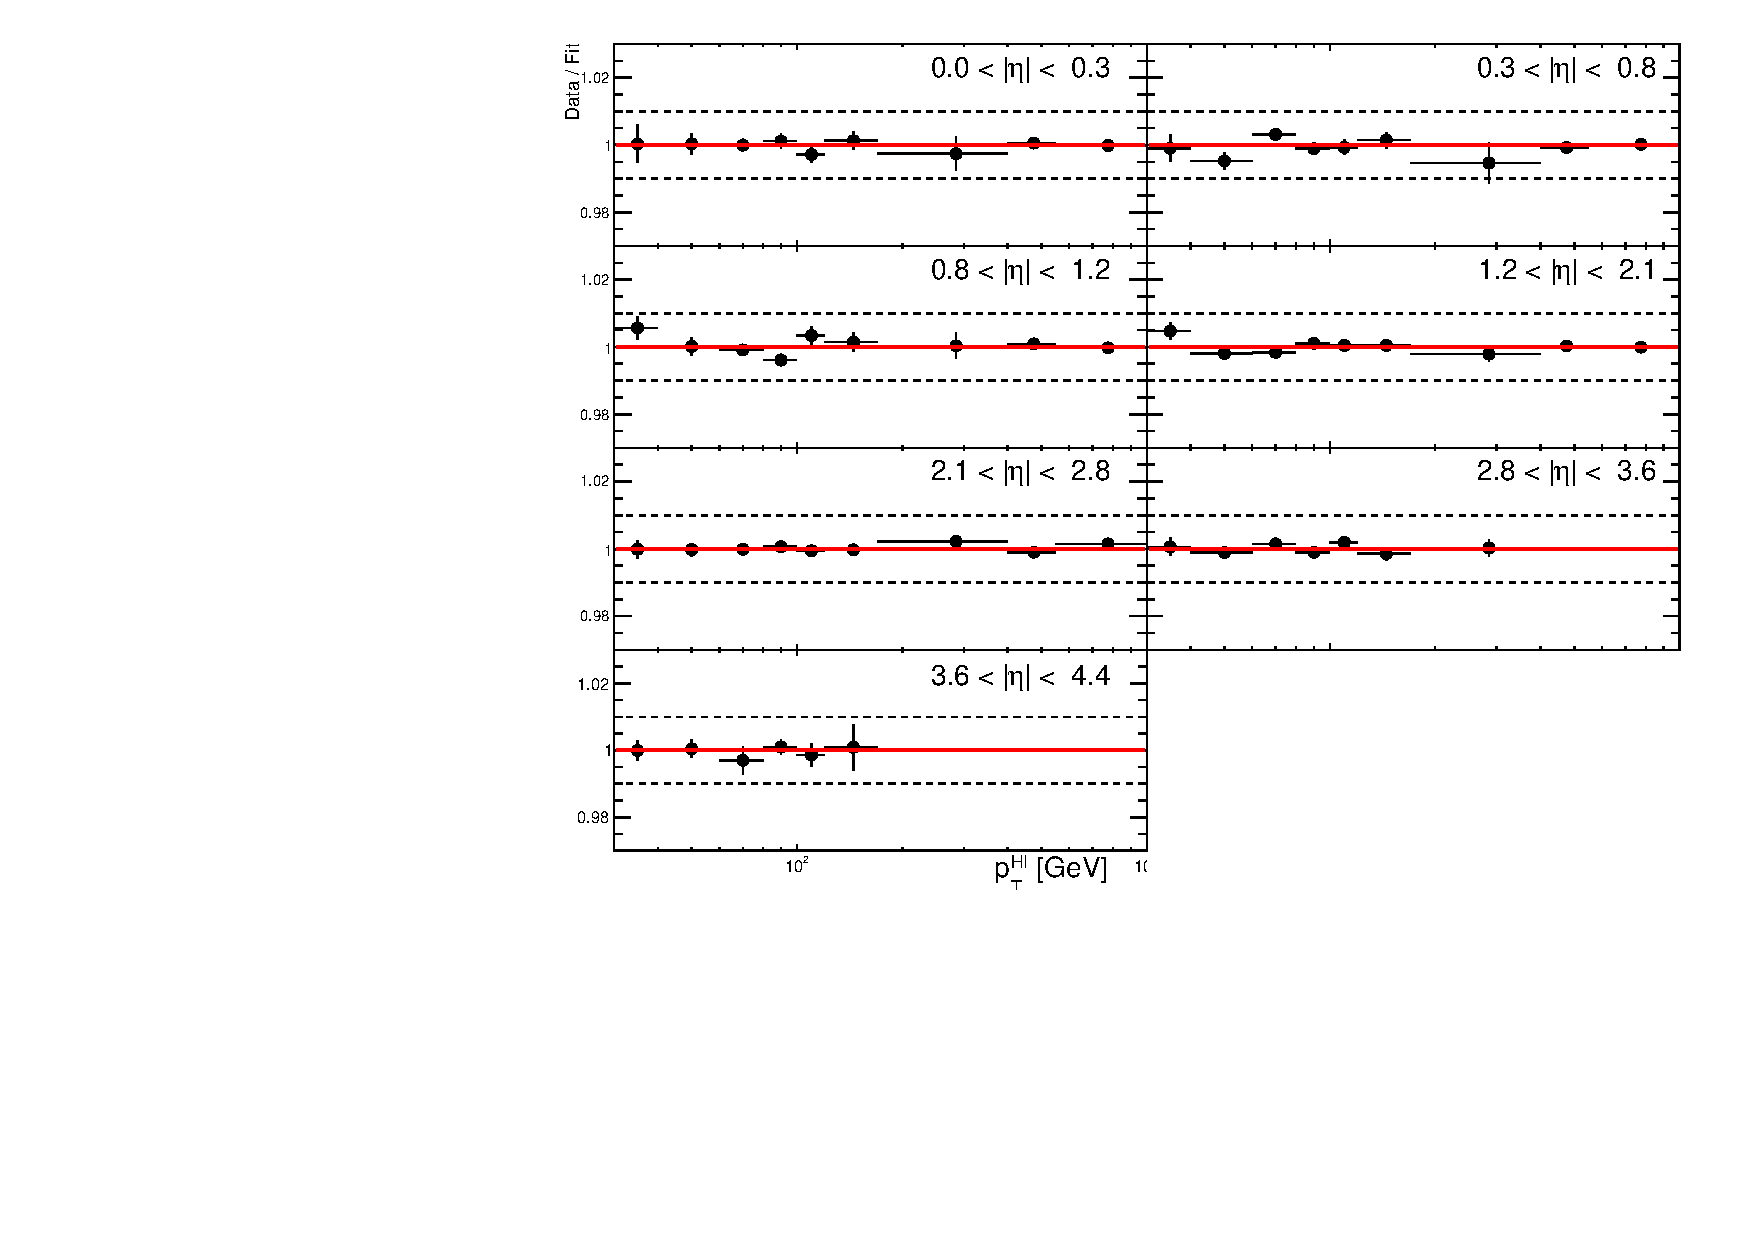
\includegraphics[width=0.5\textwidth]{figures/qualification/factors_data2fit} \\
      \end{tabular}
      }
\caption{The cross calibration factors, obtained from taking a ratio of the relative response in data and MC. A ratio of the data to the fit is given on the right}
\label{fig:cc_factors}
\end{figure}


%-------------------------------------------------------------------------------
\section{Uncertainties}
\label{sec:qual_uncertainties}
%-------------------------------------------------------------------------------

%---
\subsection{Cross calibration factor uncertainties}
\label{sec:qual_ccuncertainties}
%---


The statistical uncertainties come from the fits (using TVirtualFitter), whereas the systematics come from changing the parameters of the jet isolation criteria. These are summarized in Table~\ref{table:systematics_param}. Having a moderate nominal\ \pT \ cut on the isolation ensured that fluctuations in the HI reconstructed jets did not veto good jets. The \ \pT \ cut was also determined by the minimum\ \pT \ reconstructed by the reconstruction algorithms. The range of fits from this parametrization are shown in Fig.~\ref{fig:systematics}. The systematical uncertainties, evaluated as the maximum absolute difference between the nominal fit and any other iteration, are show in in Fig.~\ref{fig:sys_uncert}.

\begin{table}[h]
\caption{The isolation and matching parameters were varied to get the systematics. See Fig.~\ref{fig:systematics}}
\begin{tabular}{c c c c c c c c c c c}
\centering
 & \multicolumn{2}{c}{Nominal} & \multicolumn{2}{c}{Iteration 1} & \multicolumn{2}{c}{Iteration 2} & \multicolumn{2}{c}{Iteration 3} & \multicolumn{2}{c}{Iteration 4} \\
    \midrule
Isolation & R & \ \pT \ [GeV] & R & \ \pT \  [GeV] & R & \ \pT \ [GeV] & R & \ \pT \ [GeV] & \ \pT \ [GeV] \\
    \midrule
AntiKt4EMTopo		& 1.0 & 20.0 & 1.0 & 16.0 & 1.0 & 18.0 & 1.0 & 25.0 & 30.0\\
AntiKt4HI 			& 1.0 & 20.0 & 1.0 & 16.0 & 1.0 & 18.0 & 1.0 & 25.0 & 30.0\\
Truth  			& 0.6 & 20.0 & 0.6 & 16.0 & 1.0 & 18.0 & 0.6 & 25.0 & 30.0\\
    \bottomrule
    \label{table:systematics_param}
\end{tabular}
\end{table}

\begin{figure}
	\centering
	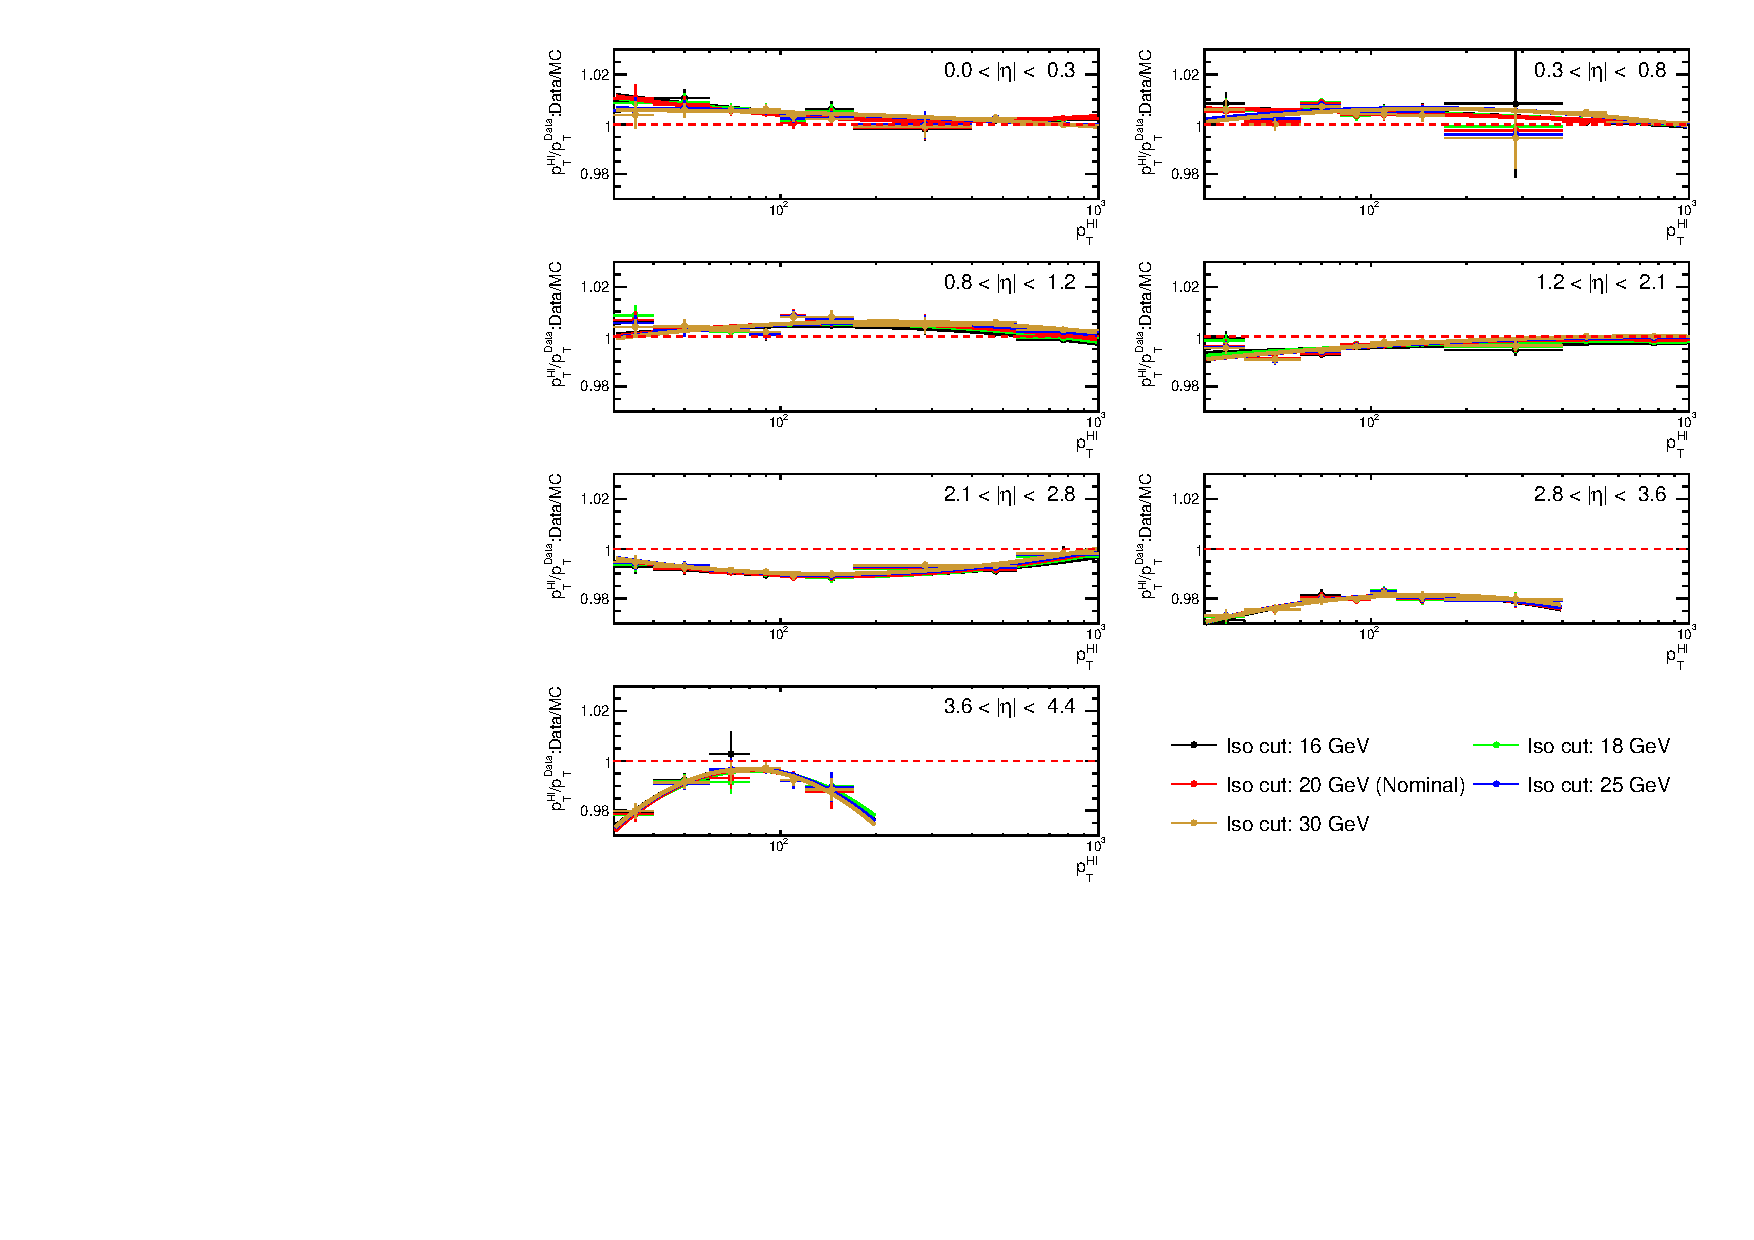
\includegraphics[width=1.0\textwidth]{figures/qualification/systematic_range}
	\caption{The fits to the cross calibration factors, with different isolation/matching cuts, as specified in Table~\ref{table:systematics_param}.  }
	\label{fig:systematics}%
\end{figure}

\begin{figure}
	\centering
	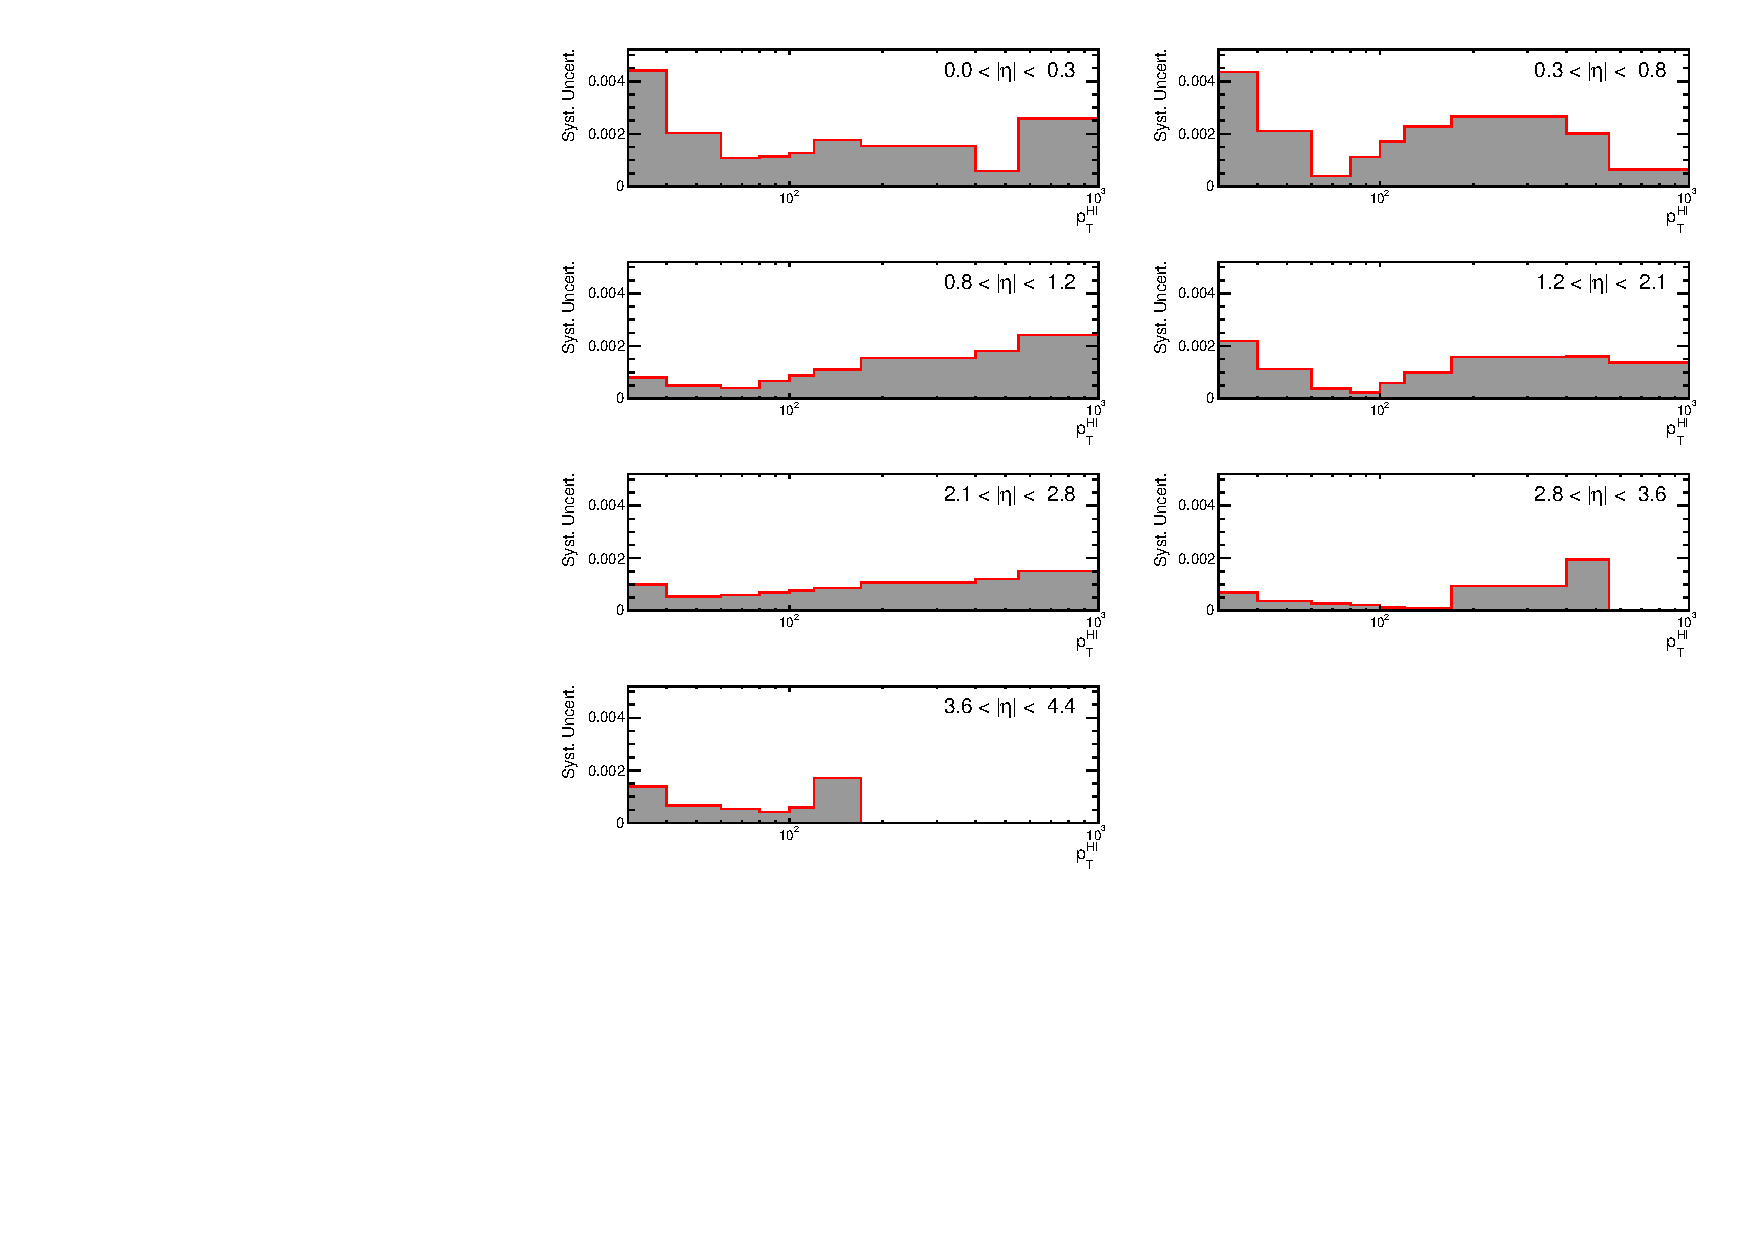
\includegraphics[width=1.0\textwidth]{figures/qualification/sys_uncert}
	\caption{The systematic uncertainty, equal to maximum difference between the nominal fit and the fits from varying the parameters (as summarized in Table~\ref{table:systematics_param}).  }
	\label{fig:sys_uncert}%
\end{figure}


%---
\subsection{Uncertainties on HI JER}
\label{sec:qual_jeruncertainties}
%---
The uncertainties on the heavy ion jet energy resolution ($\dsigma_\hi$ ) can be shown to be given by: 
\begin{align}
\dsigma_{\hi} = \frac{\delta R_{\hi}}{2 \sigma_{\hi}}
\end{align} 
where $R_\hi = \sigma_\hi^2$. We also can also derive (see \ref{sec:appendix_hijerDerivation} for derivation):
\begin{align}
\delta^2 R_\hi &= \lambda^4 \delta^2 R_\emt + \delta^2 B \\
\delta R_\emt  &= 2 \sigma_\emt \dsigma_\emt \\
\lambda &= \frac{\mathrm{Cov}(\Delta \pT^\emt | _\mathrm{noGSC}, \Delta \pT^\hi)}{\mathrm{Cov}(\Delta \pT^\emt | _\mathrm{GSC}, \Delta \pT^\hi)} \label{eq:lambda} \\ 
\delta B &= \sigma(\pT^\hi/\pt^\emt)_\mathrm{data} - \sigma(\pT^\hi/\pt^\emt)_\mathrm{MC} 
\end{align} 

$\sigma_{\emt}$ and $\dsigma_{\emt}$ were evaluated using the JER tool \cite{JERTool}, whereas $\sigma_\hi$ was measured in the data (shown in Fig~\ref{fig:emtopo_jer}. $\lambda$ was determined using $\Delta\pT^\emt = \pT^\emt - \pT^\tru$ and $\Delta\pT^\hi =\pT^\hi - \pT^\tru$ evaluated with and without the GSC calibration. 

Fluctuations in $\sigma_\emt$ and $\sigma_\hi$ were removed by fitting to the form
\begin{align}
a+(b/\pT)+(c/\pT)^2
\label{fit:jer_fit}
\end{align}
These are shown in Fig.~\ref{fig:fitted_jer}. The $\Delta\pT^\emt$ vs. $\Delta\pT^\hi$ for with and without the GSC can be seen in Fig.~\ref{fig:deltapT_w_gsc} and Fig.~\ref{fig:deltapT_no_gsc} respectively. The $\lambda$ distribution can be seen in Fig.~\ref{fig:lambda}. A comparison between $\delta\sigma_\emt$ and $\delta\sigma_\hi$ can be seen in Fig.~\ref{fig:meth2_jer_uncert}. The ratio $\delta\sigma_\emt / \delta\sigma_\hi$ can be expressed as below:
\begin{align}
\frac{\delta\sigma_\hi}{\delta\sigma_\emt} = \frac{\delta R_\hi}{\delta R_\emt} \frac{\sigma_\emt}{\sigma_\hi}
\end{align}
This factorization (plotted in Fit.~\ref{fig:meth2_ratios}) showed that the large differences between $\delta\sigma_\emt$ and $\delta\sigma_\hi$ were coming from the differences in the uncertainties, as opposed to differences in the actual resolutions themselves. The same quantity, $\delta\sigma_\emt / \delta\sigma_\hi$, as calculated in Run I is shown in Fig.~\ref{fig:run1_jer_uncert} \cite{xcalib_run1}.





\begin{figure}
    \centering
        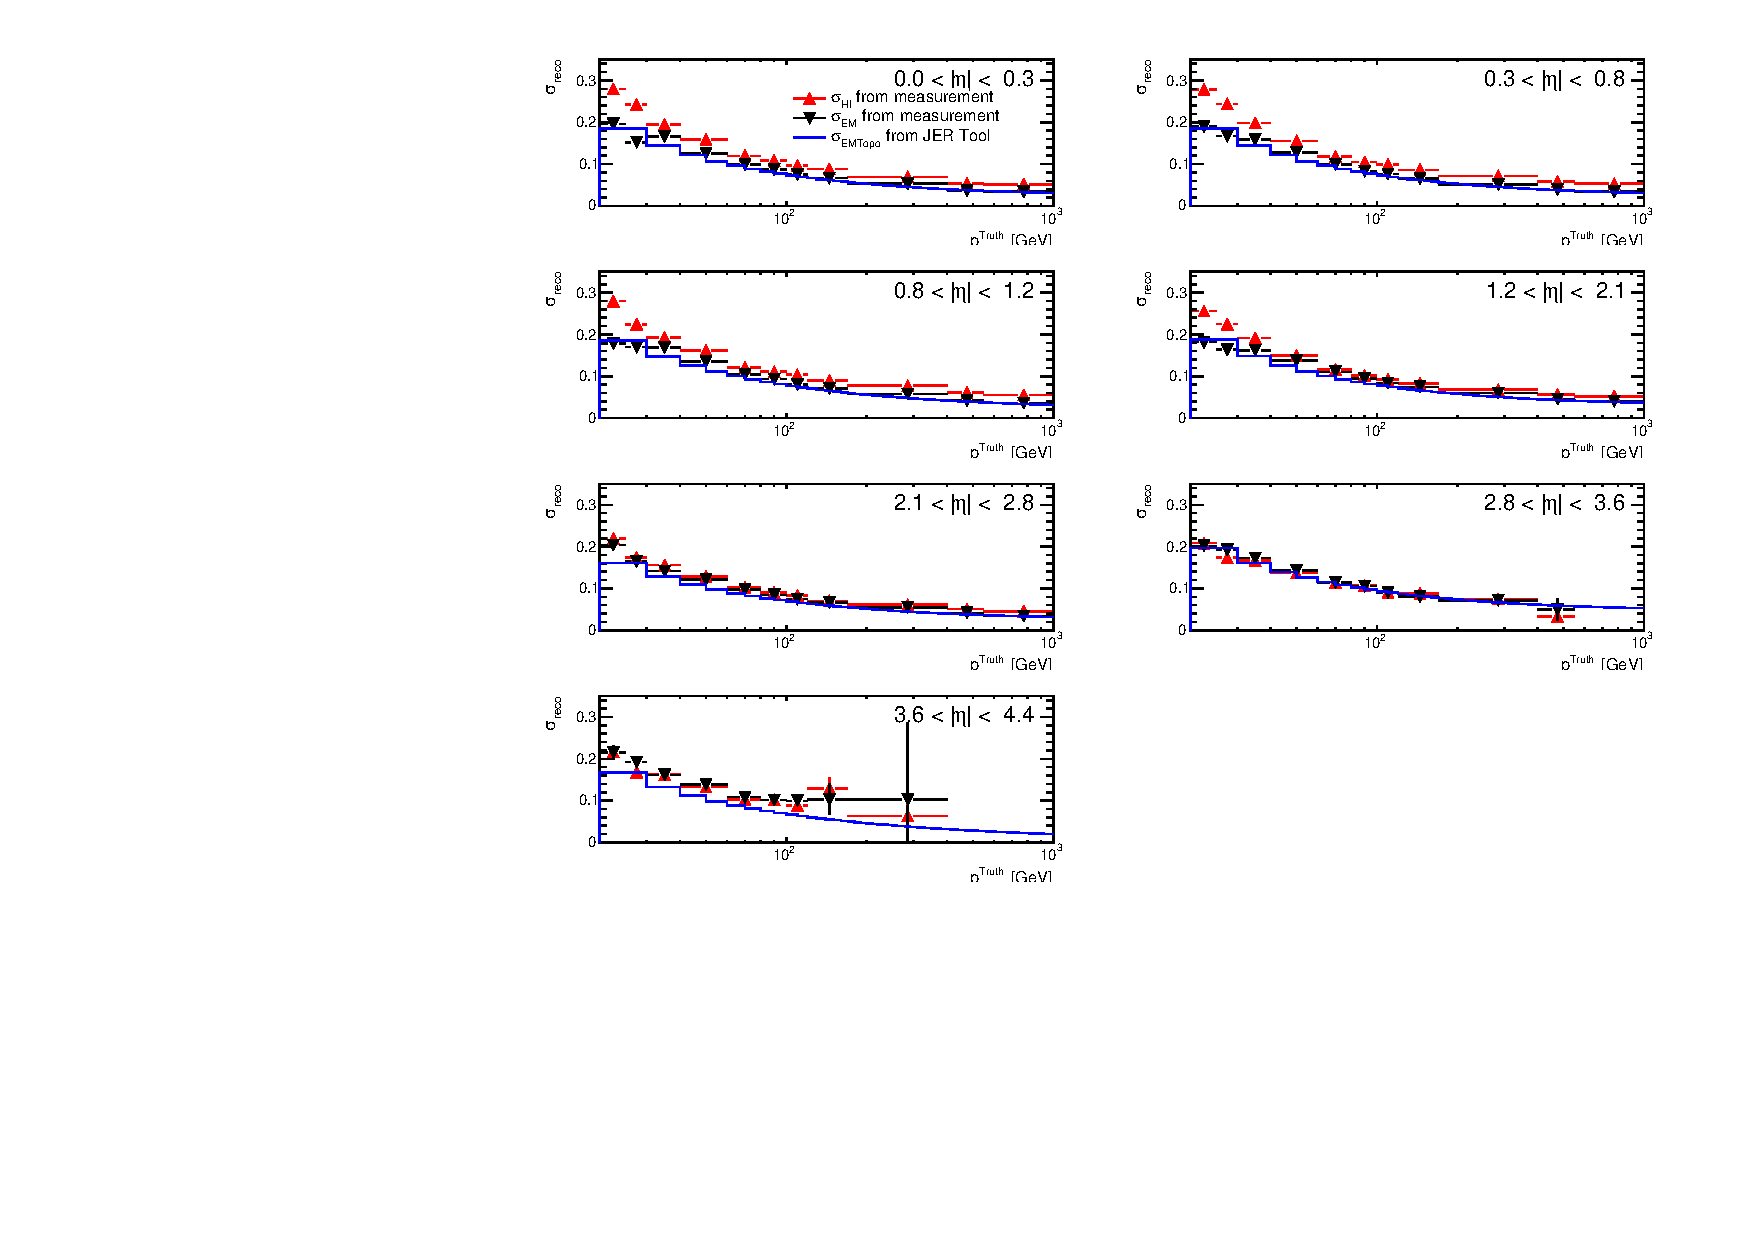
\includegraphics[width=1\textwidth]{figures/qualification/emtopo_jer}
		\caption{A comparison of the JER of EMTopo and HI jets from the datasets, as well as from the JER Tool. }
		\label{fig:emtopo_jer}
    \end{figure}%

    \begin{figure}
        \centering
        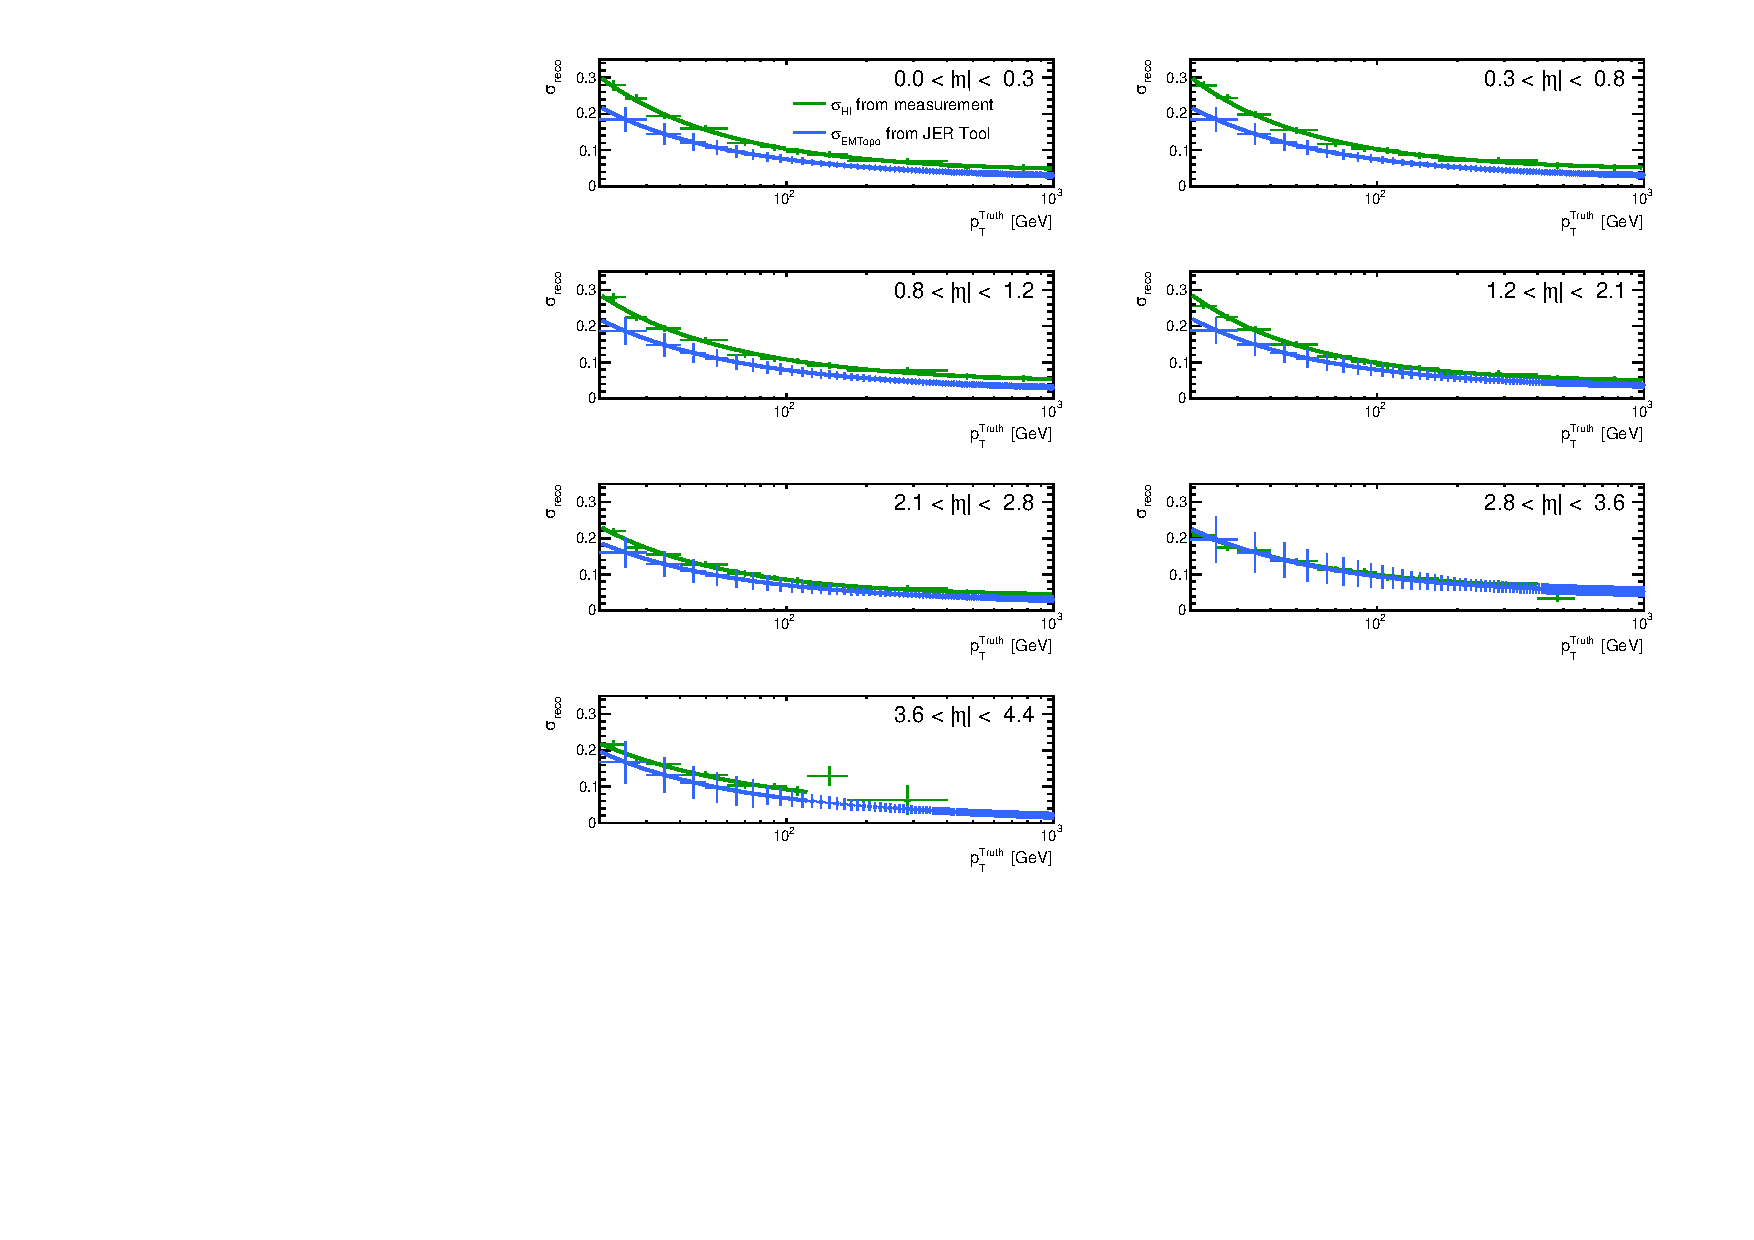
\includegraphics[width=1\textwidth]{figures/qualification/fitted_jer}
		\caption{The JER for $\hi$ and $\emt$ jets fit to Eq.~\ref{fit:jer_fit}}
		\label{fig:fitted_jer}
	\end{figure}





\begin{figure}
        \centering
        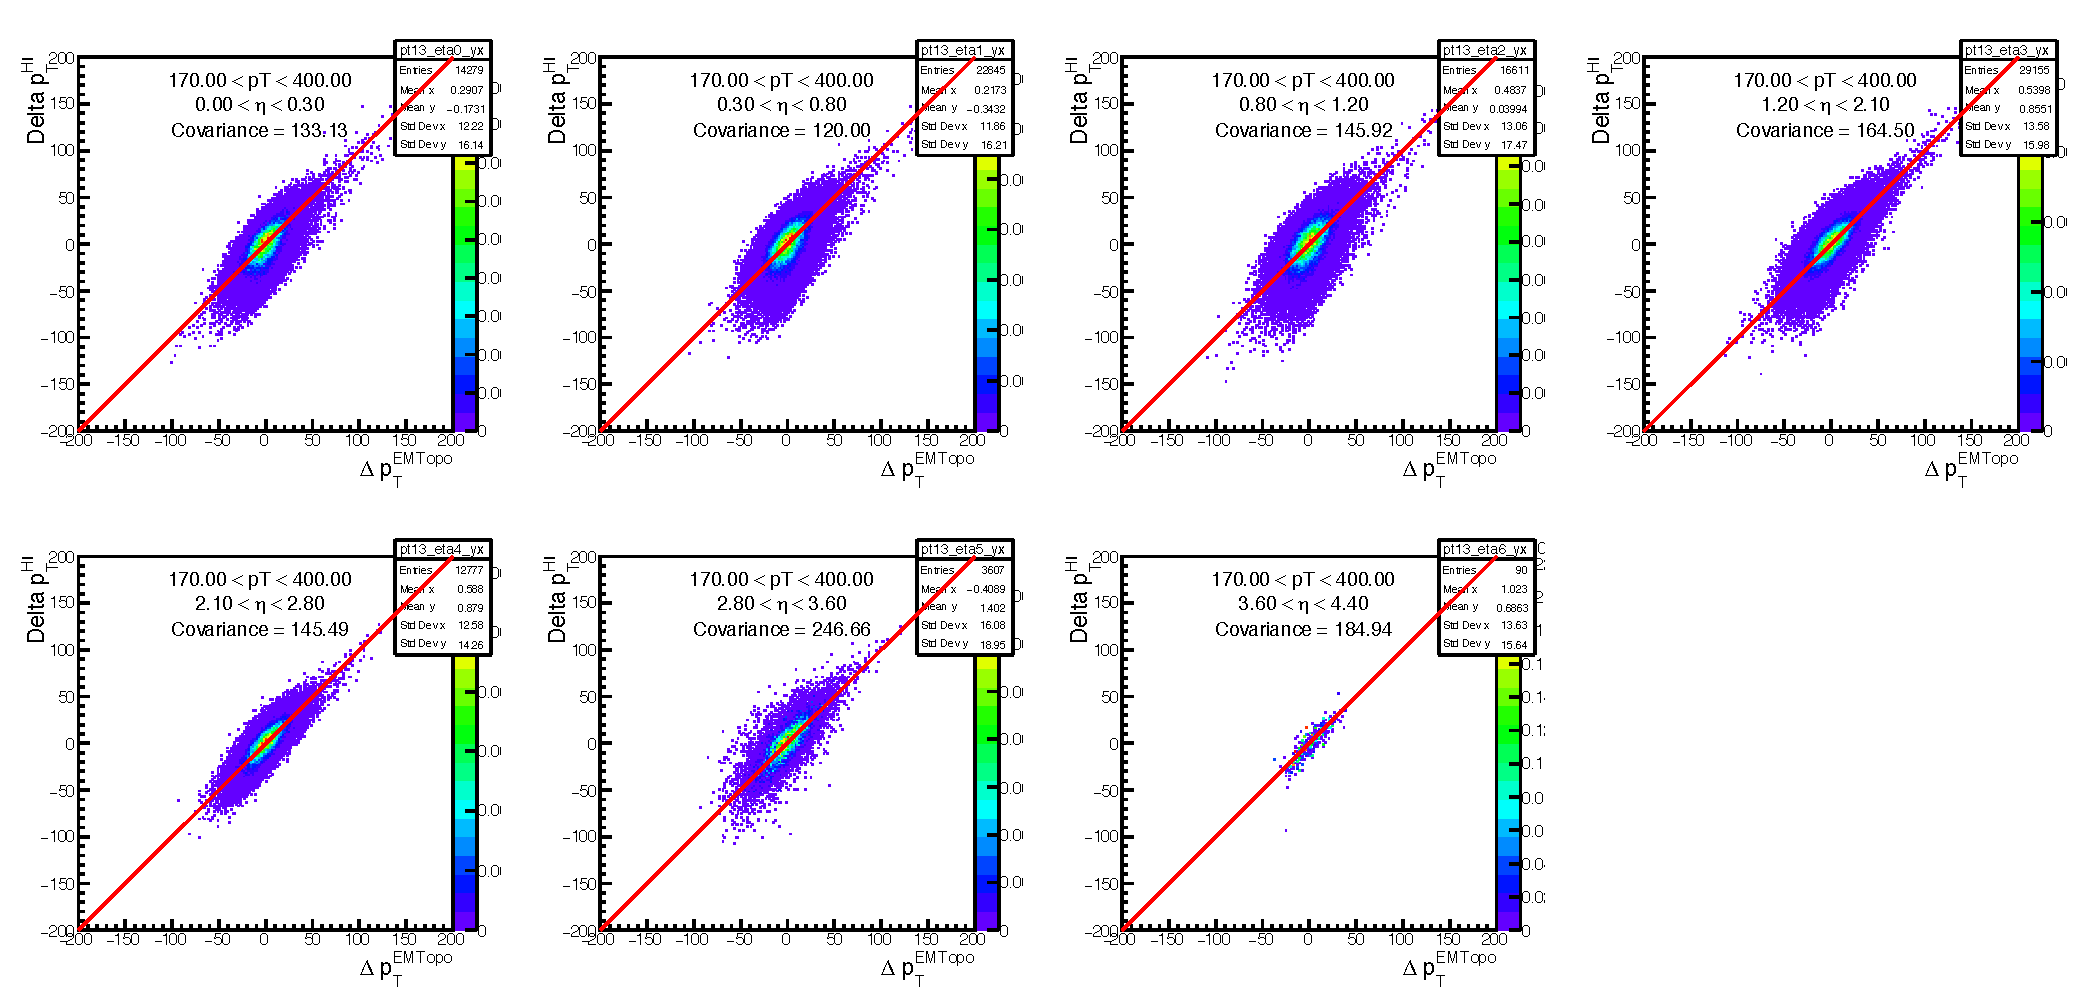
\includegraphics[width=1\textwidth]{figures/qualification/deltapT_w_gsc}
		\caption{The $\Delta\pT^\emt$ vs. $\Delta\pT^\hi$ distribution in all $\eta$ bins, for $ 170 < \pT^\tru < 400$ GeV, with the GSC calibration applied to the $\emt$ jets. }
		\label{fig:deltapT_w_gsc}
    \end{figure}%

    \begin{figure}
        \centering
        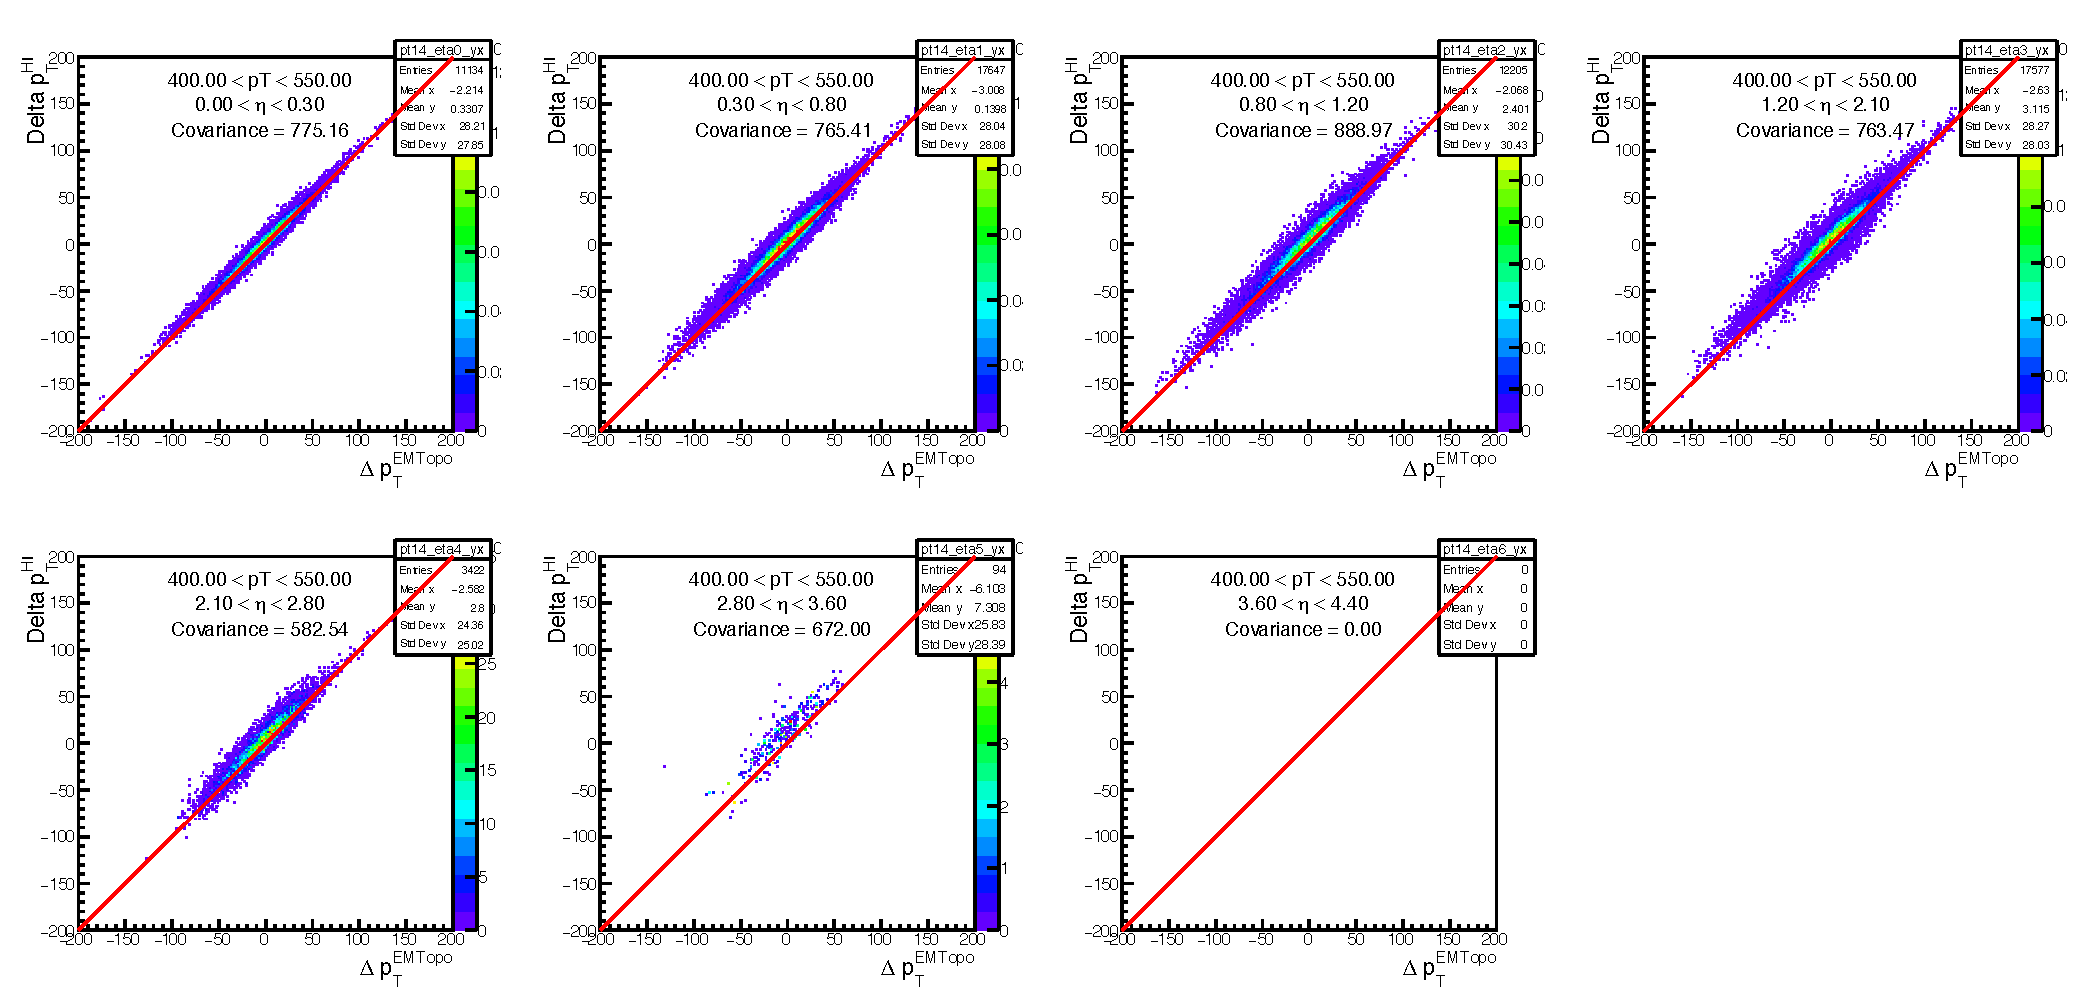
\includegraphics[width=1\textwidth]{figures/qualification/deltapT_no_gsc}
		\caption{The $\Delta\pT^\emt$ vs. $\Delta\pT^\hi$ distribution in all $\eta$ for $ 170 < \pT^\tru < 400$ GeV, with no GSC calibration applied to the $\emt$ jets. }
		\label{fig:deltapT_no_gsc}
\end{figure}




\begin{figure}
        \centering
        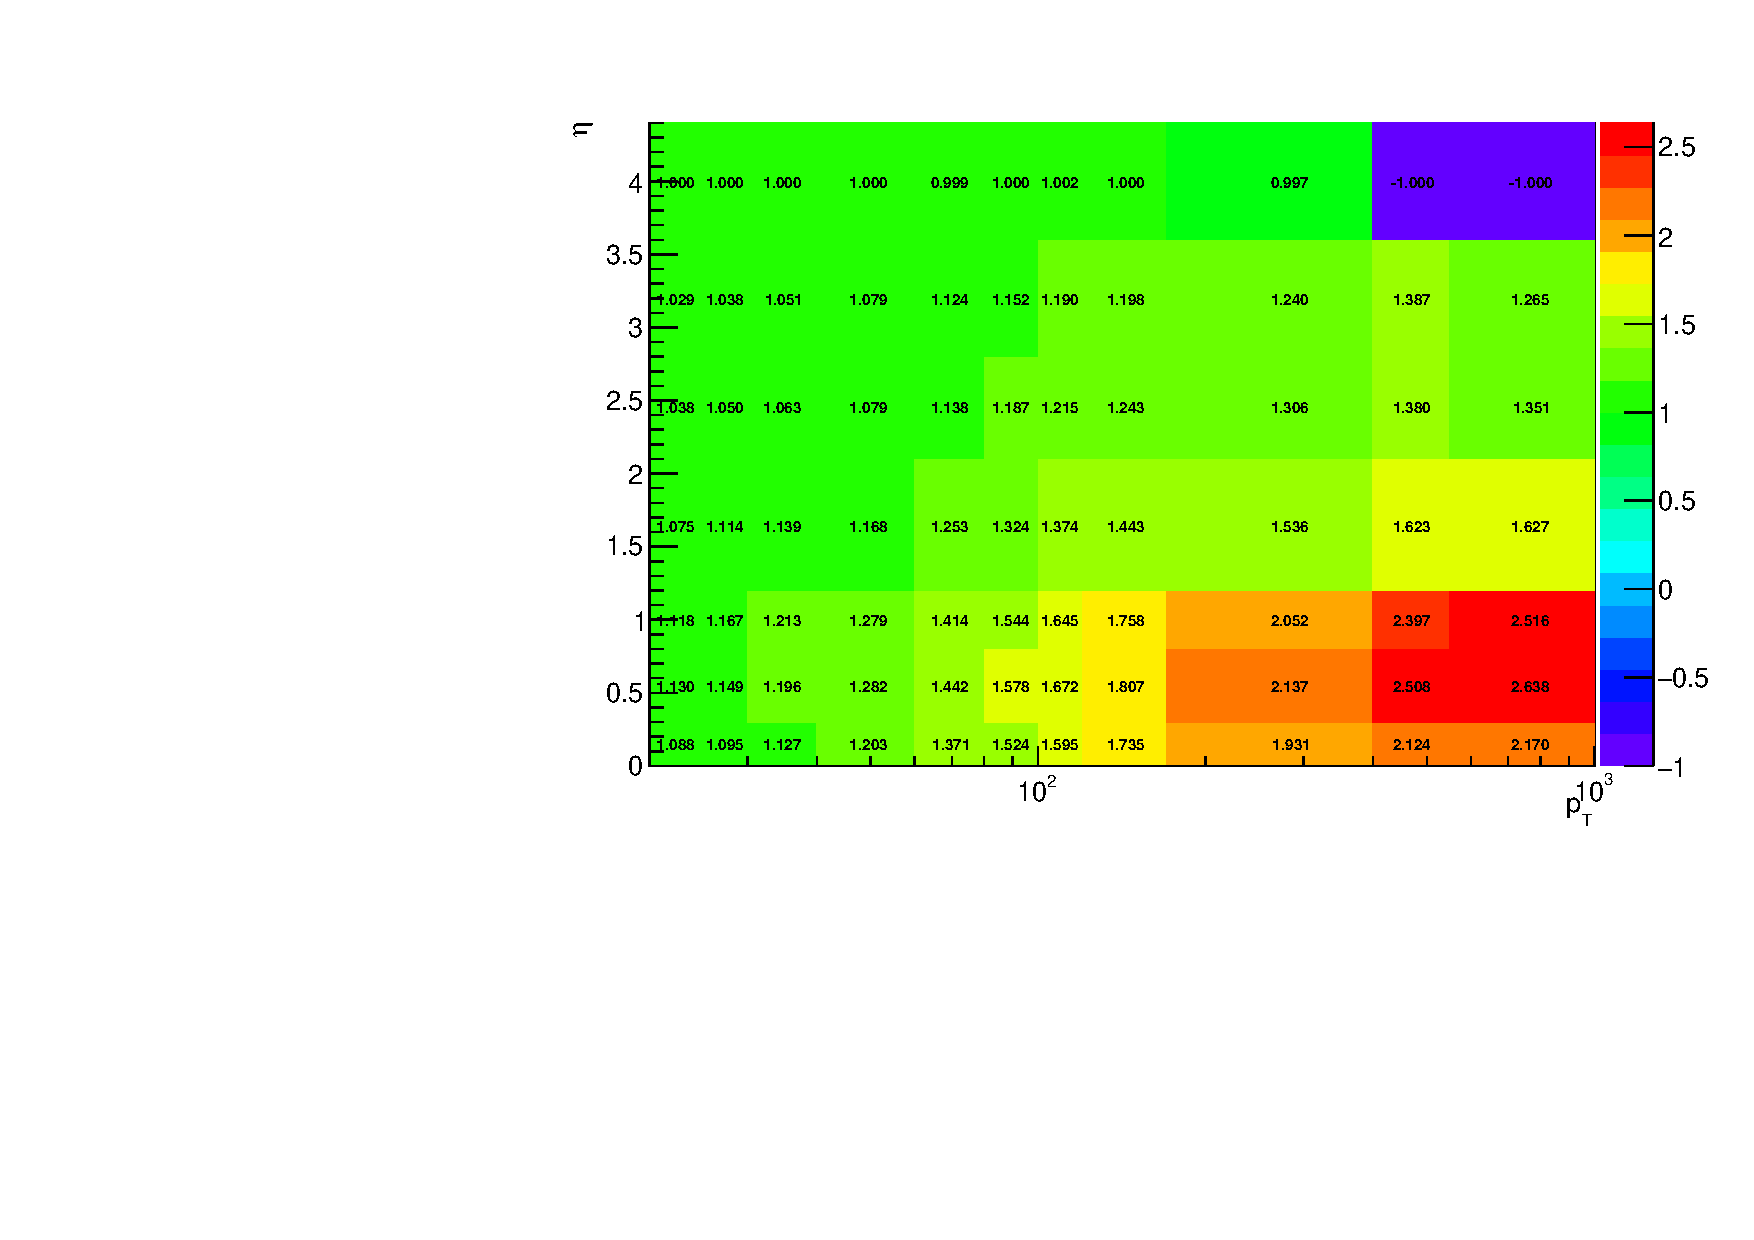
\includegraphics[width=1\textwidth]{figures/qualification/lambda}
		\caption{The distribution of $\lambda$ as calculated in Eq.~\ref{eq:lambda} in various bins of $\pt$ and $\eta$.}
		\label{fig:lambda}
    \end{figure}%

    \begin{figure}
        \centering
        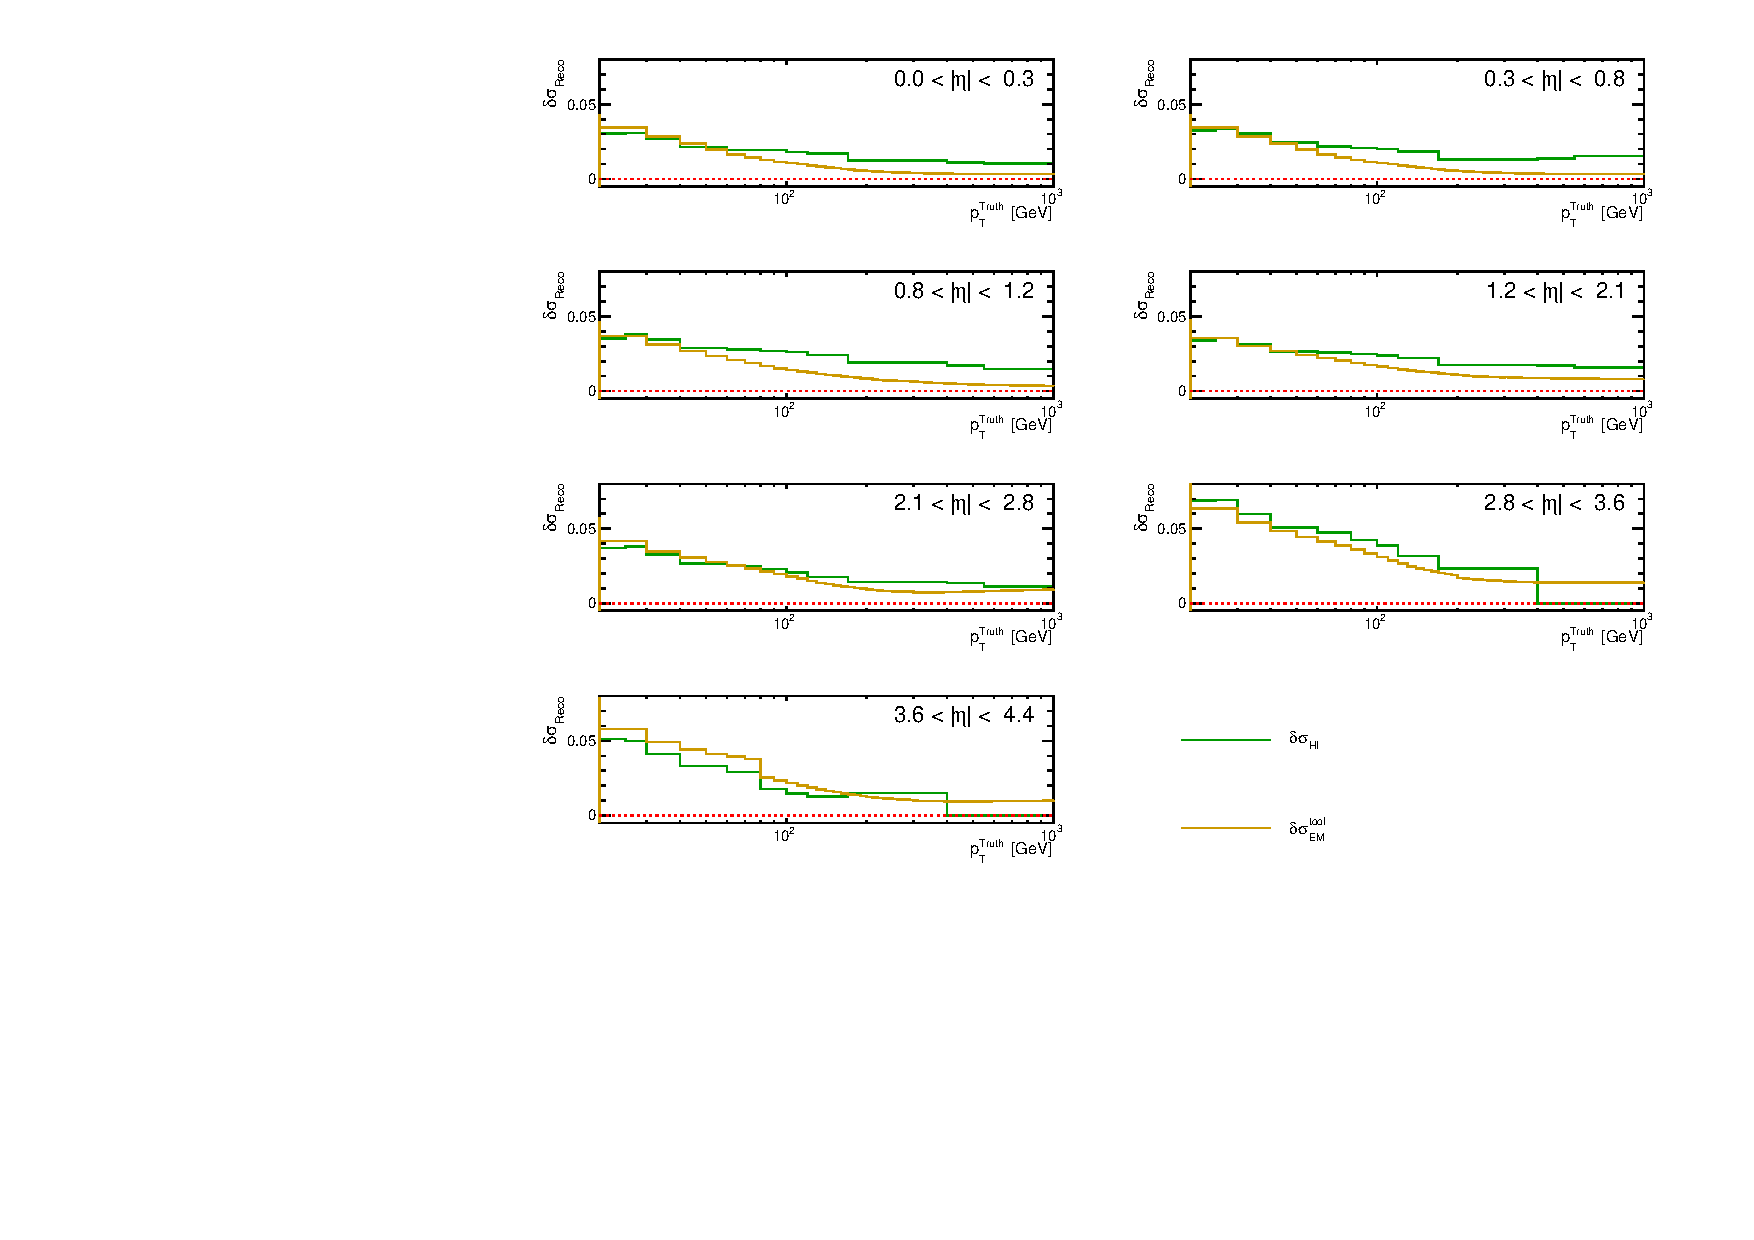
\includegraphics[width=1\textwidth]{figures/qualification/meth2_jer_uncert}
		\caption{A comparison between $\delta\sigma_\emt$ and $\delta\sigma_\hi$ in various $\eta$ bins}
		\label{fig:meth2_jer_uncert}
\end{figure}



\begin{figure}
        \centering
        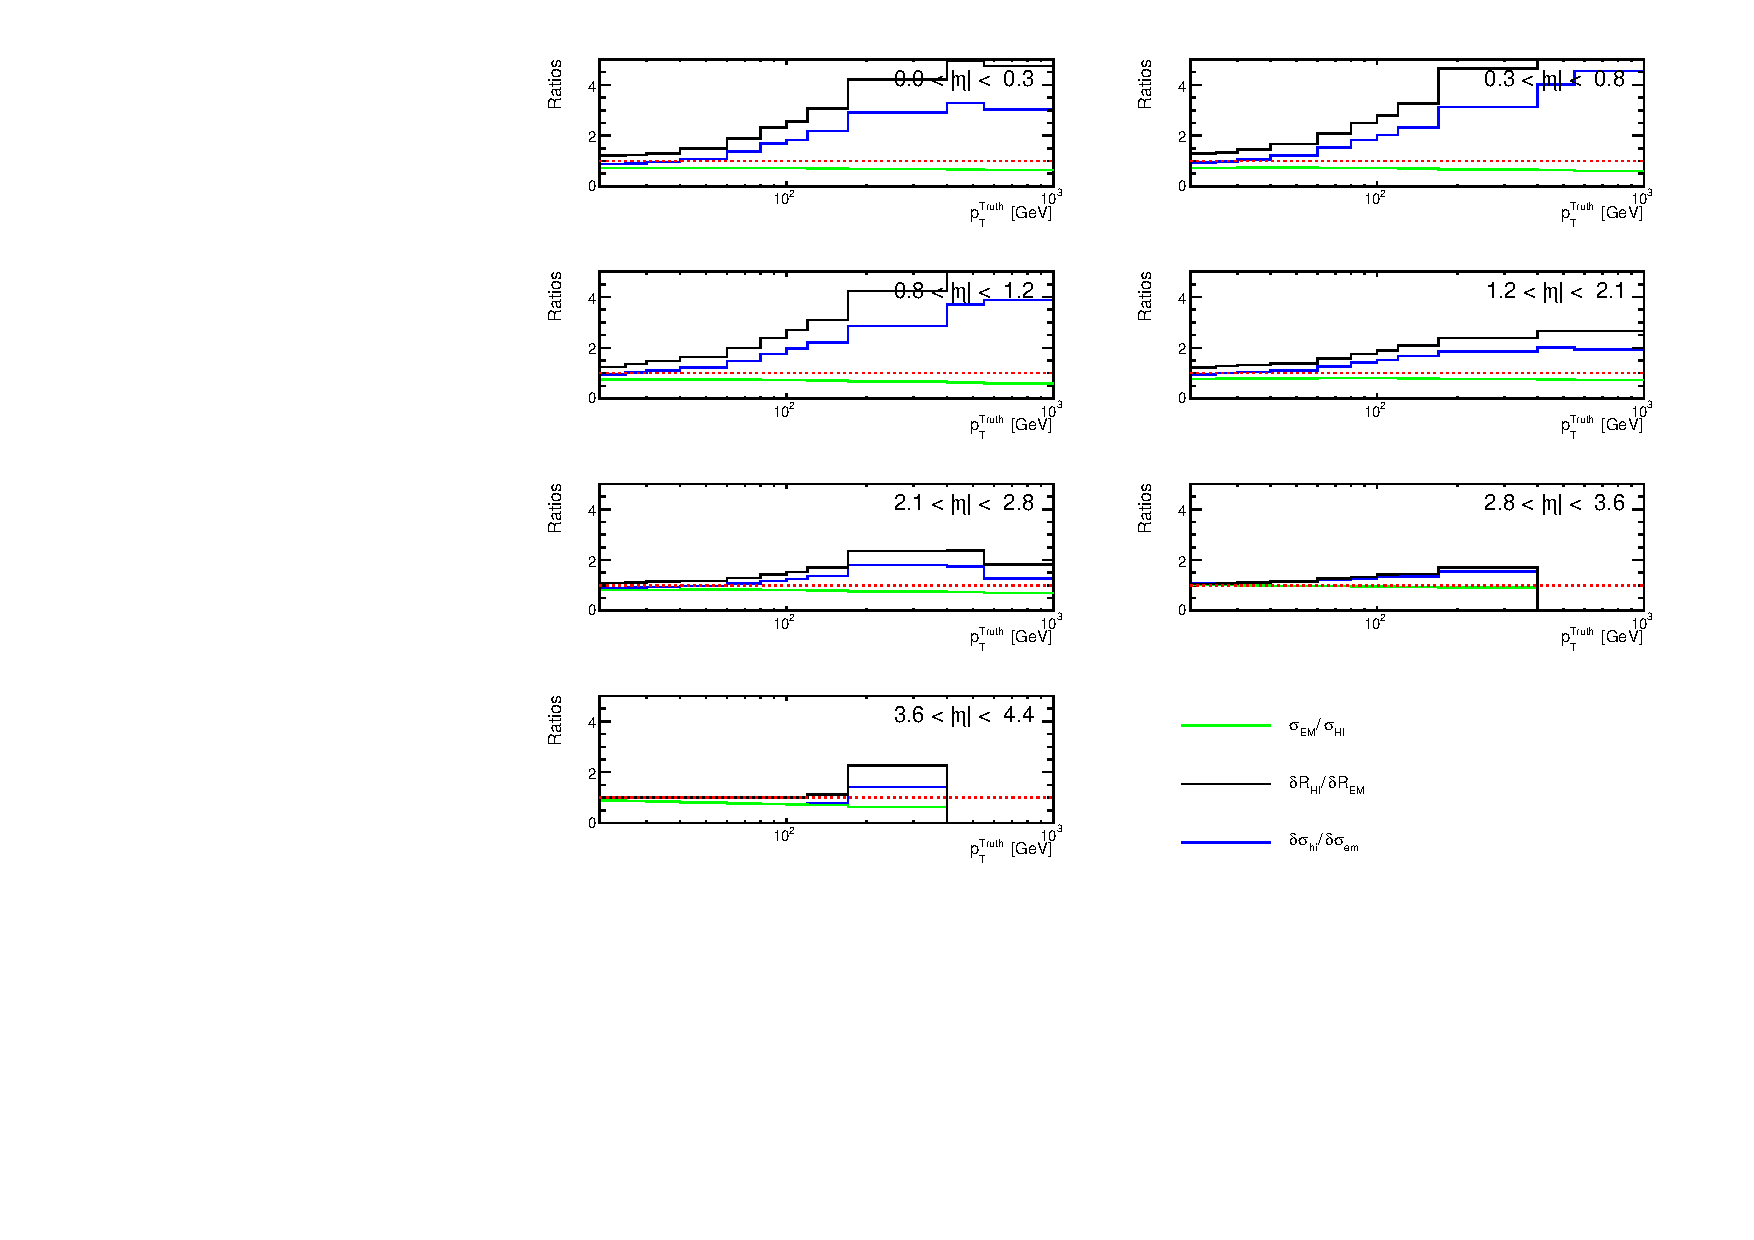
\includegraphics[width=1\textwidth]{figures/qualification/meth2_ratios}
		\caption{Factorizing the ratio $\delta\sigma_\emt / \delta\sigma_\hi$ shows that the dominant effect is from the uncertainties themselves (as opposed to a difference in the resolutions)}
		\label{fig:meth2_ratios}
    \end{figure}%

    \begin{figure}
        \centering
        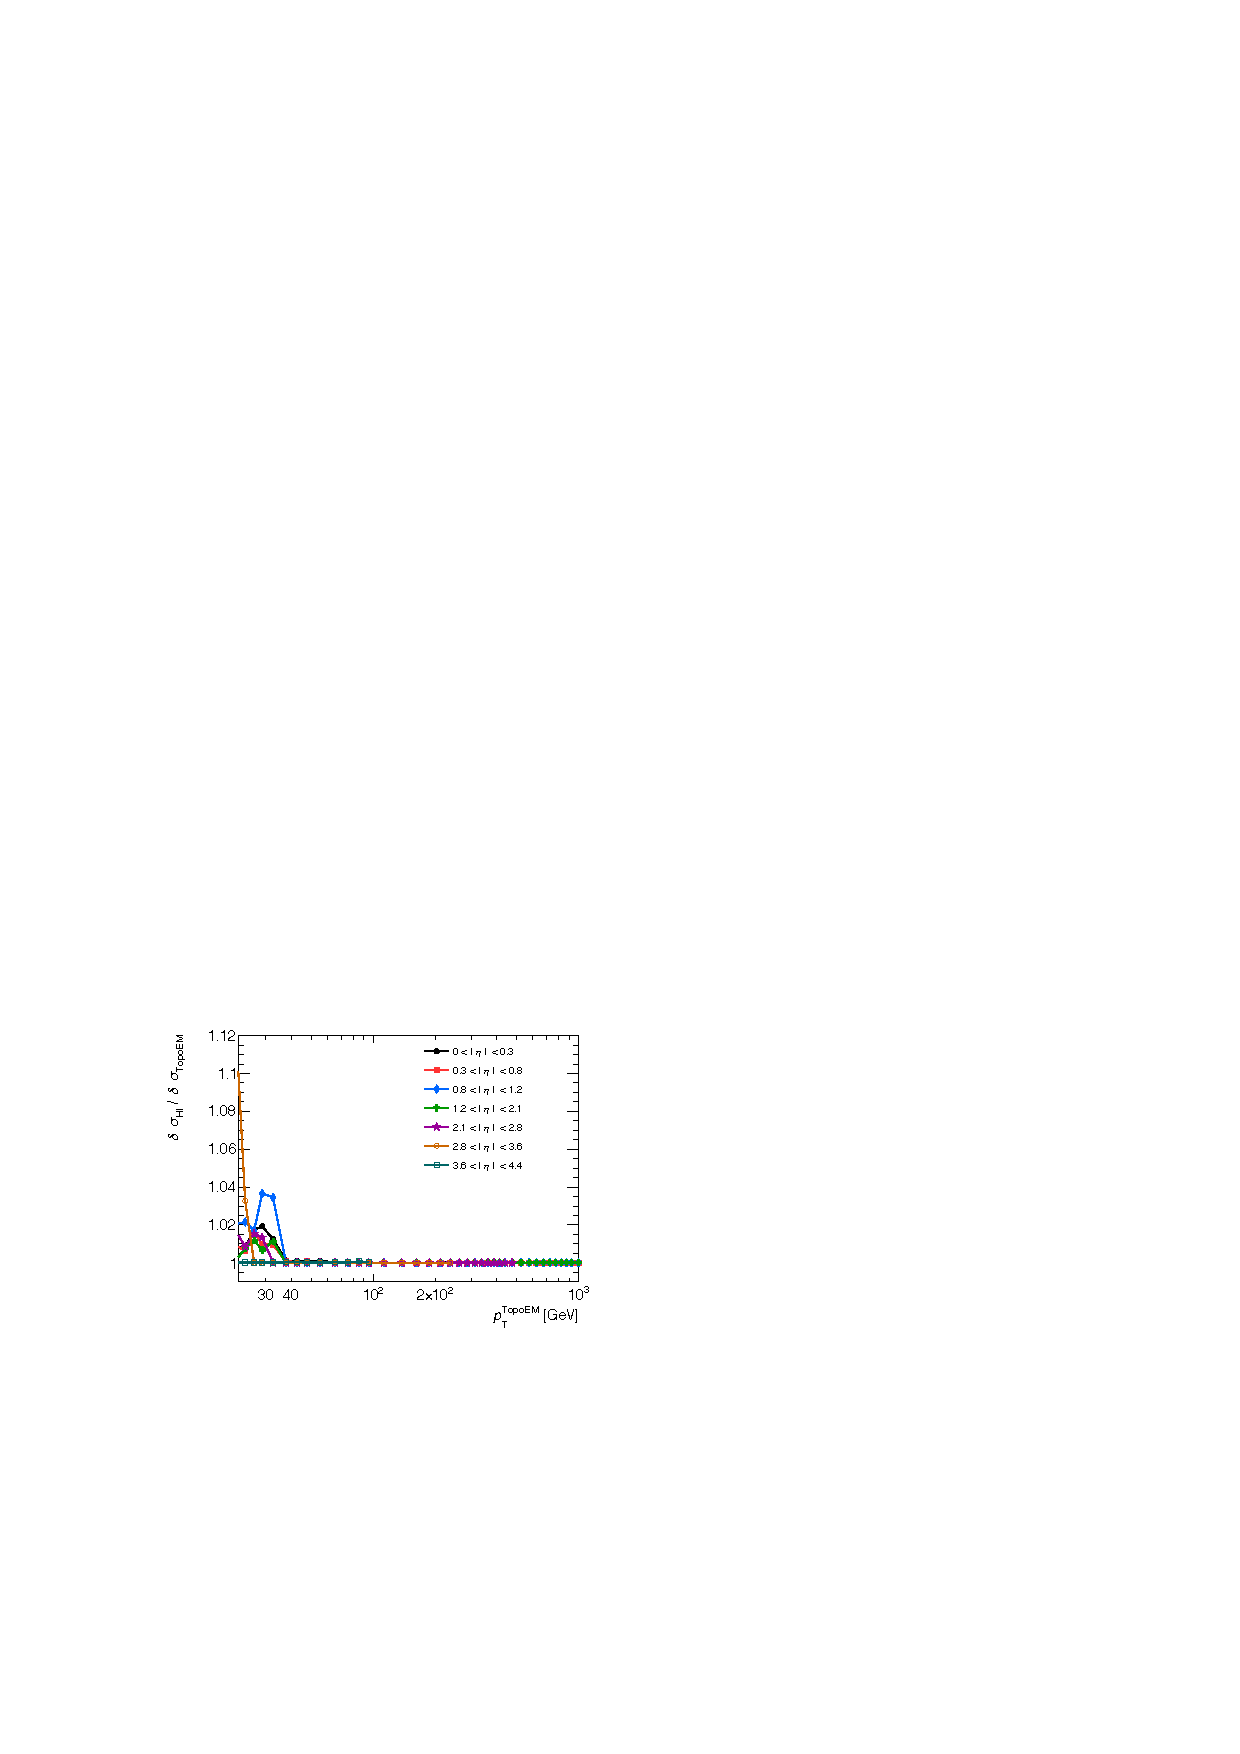
\includegraphics[width=1\textwidth]{figures/qualification/run1_jer_uncert}
		\caption{The ratio $\delta\sigma_\emt / \delta\sigma_\hi$ as evaluated in Run I \cite{xcalib_run1}}
		\label{fig:run1_jer_uncert}
\end{figure}



%-------------------------------------------------------------------------------
\section{Qualification Task Conclusion}
\label{sec:qual_result}
%-------------------------------------------------------------------------------
The cross calibration factors, along with its systematic and statistical uncertainties were derived in different $\eta$ regions, as a function of $\pT^{\hi}$, and are shown in Fig.~\ref{fig:factors_w_uncertainties}. The factors themselves are the level of ~1\%, and do not show much variation with $\pT$.  Furthermore, the uncertainties are primarily statistical in nature. 



\begin{figure}
	\centering
	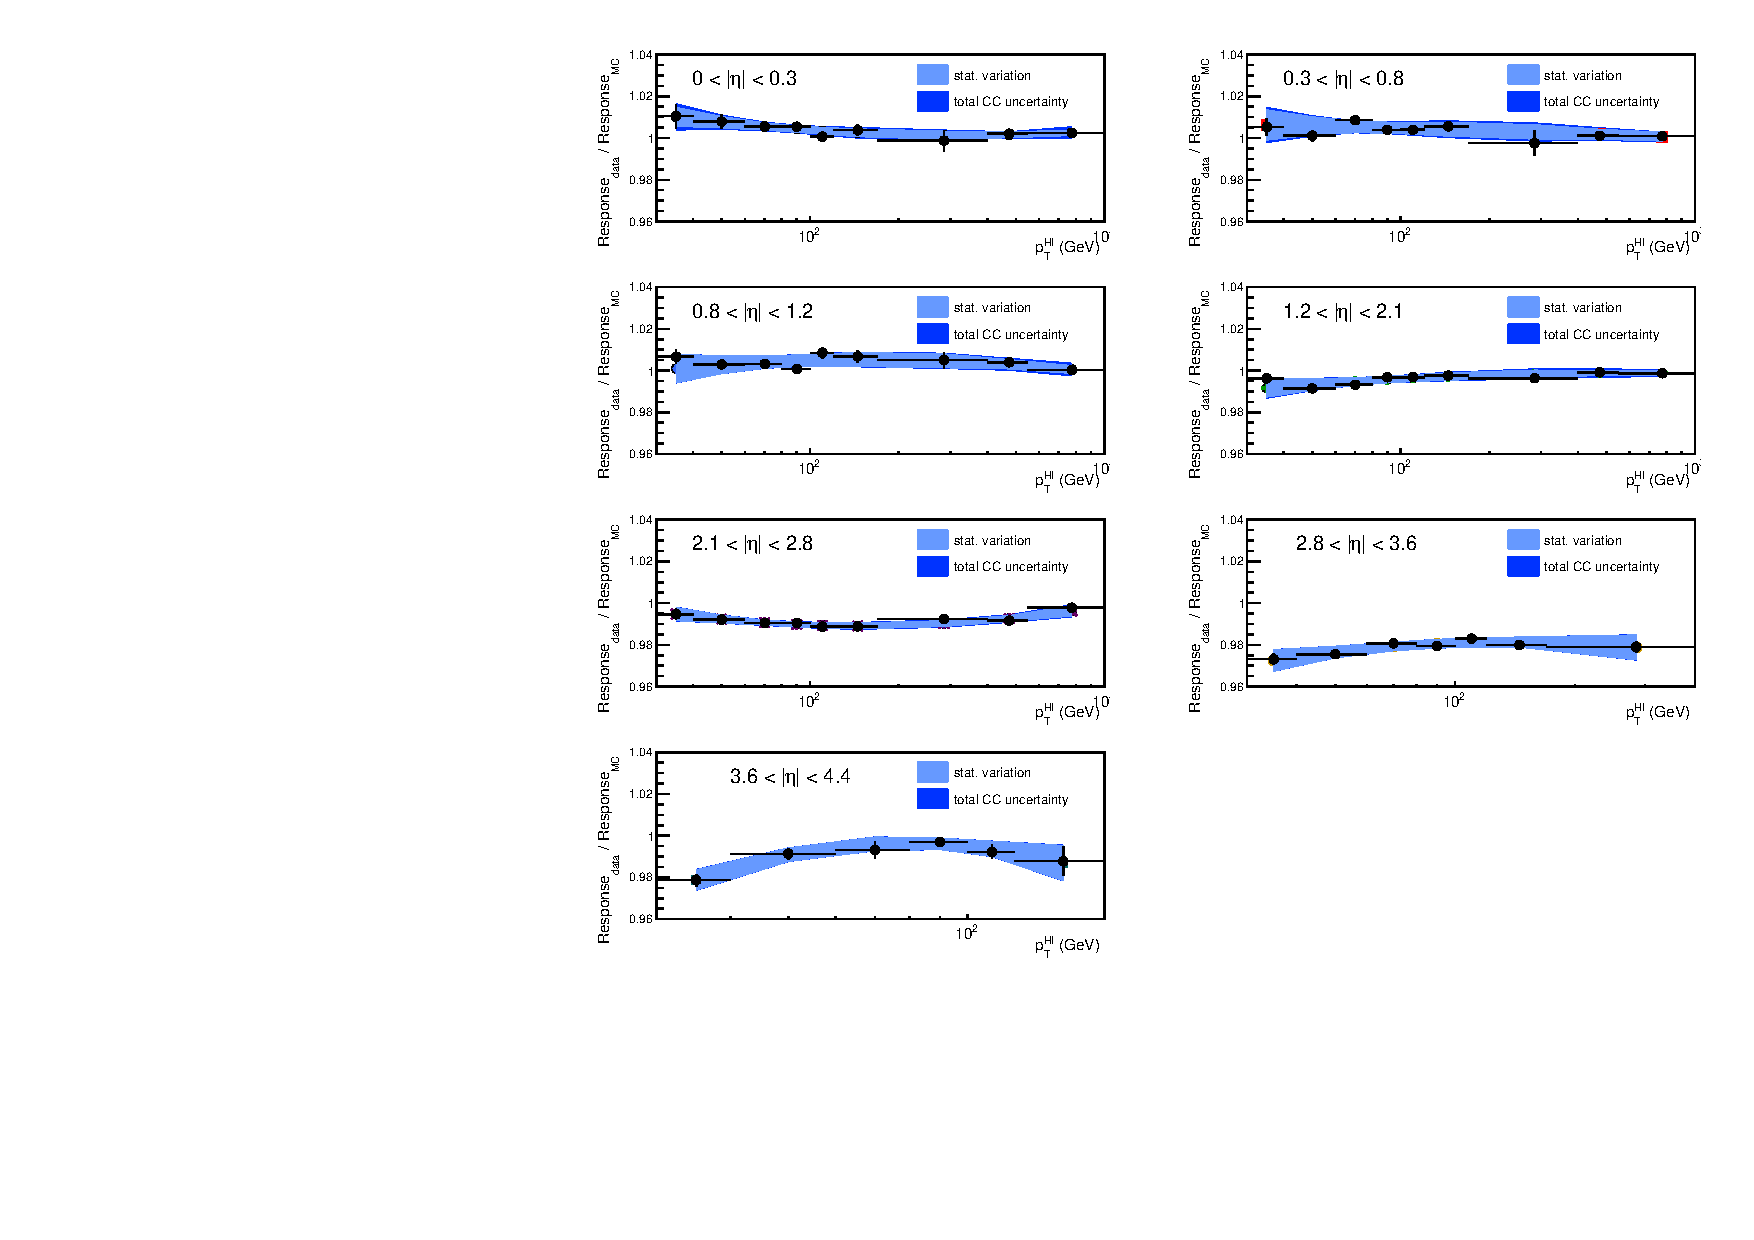
\includegraphics[width=1.0\textwidth]{figures/qualification/factors_w_uncertainties}
	\caption{The cross calibration factors in different $\eta$ regions, as a function of $\pT^{\hi}$, along with their uncertainties.}
	\label{fig:factors_w_uncertainties}%
\end{figure}

 A $\pT$ dependent uncertainty on the HI JER was also derived, and can be seen in Fig.~\ref{fig:meth2_jer_uncert}.



%%%%%%%%%%%%%%%%%%%%%%%%%%%%%
%\chapter{Measurement of Dijet Azimuthal Correlations}
%\label{sec:mainanalysis}
%\section{Overview}
%% !TEX root = thesis-ex.tex

This chapter gives a detailed outline for the analysis of azimuthal correlations in \pp\ and \pPb\ data taken with the ATLS detector. First, in Section~\ref{sec:data}, an overview of the size and type of data and simulation samples used in the analysis is given. Next, in Section~\ref{sec:event}, the rules for event selection in these respective data and MC samples are discussed. This is including but not limited to simple phase-space cuts or trigger requirements in data. Since jets are the observables used in this analysis, a detailed overview of the jet reconstruction is given in Section~\ref{sec:reconstruction}. As with all analysis done in ATLAS, the proper performance of the detector must be verified before the beginning of the physics measurement. Any irregularities that are identified must later be corrected for in order to have a proper physics measurement. Detector performance is evaluated using MC samples and is later used as input into any known systematics that should be taken into account for a precise physics measurement. Next, in Section~\ref{sec:analysis}, the main analysis procedure is described. This section goes step-by-step through all parts of the analysis, explaining why things were done, and backs up every part with respective plots. Systematic uncertainties, which are very important and a large part of the analysis are presented in Section~\ref{sec:systematics}. Finally, everything is put together and the results and discussion of the measurements are presented in Section~\ref{sec:results}. A summary of these analysis steps, with their respective sections are below:

\begin{itemize}
	\item Data sets - Section~\ref{sec:data}
	\item Trigger and Event Selection - Section~\ref{sec:event}
	\item Jet Selection and Reconstruction Performance - Section~\ref{sec:reconstruction}
	\item Analysis Procedure - Section~\ref{sec:analysis}
	\item Systematic Uncertainties- Section~\ref{sec:systematics}
	\item Results - Section~\ref{sec:results} 
\end{itemize}

\newpage

%%%%%%%%%%%%%%%%%%%%%%%%%%%%%
%\section{Data Sets}
%\label{sec:data}
%% !TEX encoding = UTF-8 Unicode
% !TEX root = thesis-ex.tex

The \pPb\ data used in this analysis were recorded in 2016 and the samples used are shown in Table~\ref{tab:datasamples} in the appendix. The LHC was configured with a 4 TeV proton beam and a 1.57~TeV per nucleon Pb beam  producing collisions with \sqrtsnn~=~5.02~TeV and a rapidity shift of the  nucleon-nucleon center-of-mass frame $\Delta y=-0.465$ relative to the lab frame. The data collected had one beam configuration with the Pb beam traveling to the positive pseudorapidity direction and the proton beam to the negative pseudorapidity direction. To be consistent with previous \pPb\ physics measurements~\cite{ATLAS:2014cpa,Aaboud:2017tke}, the positive center-of-mass rapidity direction, $\ystar>0$ is chosen as the proton beam direction. The physical detector is described in terms of $\eta$ and is consistent with conditions used during data-taking while the center-of-mass rapidity \ystar\ is the physics quantity in which results are presented. The integrated luminosity of the 2016 \pPb\ data taken is 360~\mubarn$^{-1}$. The \pp\ data used in this measurement was recorded in 2015 with the LHC configured to collide two equal energy proton going beams at a center-of-mass energy of \sqrts~=~5.02~TeV. These \pp\ and \pPb\ data samples are shown in Table~\ref{tab:datasamples} in the appendix. The instantaneous luminosity conditions provided by the LHC during \pPb\ data taking resulted in an average number of interactions per bunch crossing of 0.03. During \pp\ data taking, the average number of interactions per bunch crossing varied from 0.6 to 1.3. 

The performance for measuring azimuthal angular correlations and conditional yields in both the 2015  \pp\ and 2016 \pPb\ data samples is evaluated with a 5.02~TeV \pp\ MC sample simulated using \pythia\ 8.212~\cite{Sjostrand:2014zea}. Hard scattering \pp\ events with the A14~\cite{ATLAS2014021} tune and the next-to-next order NNPDF23LO PDF set~\cite{Ball:2012cx} are used. The detector response is then simulated using GEANT4~\cite{Agostinelli:2002hh,Aad:2010ah}. The \pp\ samples used for this analysis contain approximately 12 million events, and are listed with their respective number of events in the top Table~\ref{tab:mcsamples} in the appendix. Corresponding \pPb\ MC samples are obtained by overlaying minimum-bias \pPb\ data events recorded during the 2016 data-taking period with simulated 5.02~TeV \pp\ events generated with the same MC tune as for the \pp\ MC sample but with a rapidity shift equivalent to that in the \pPb\ collisions. Detector response is also modeled using GEANT4. Due to the forward rapidity filtering, approximately 3 million events were used in the \pPb\ MC samples. These samples are listed in the middle of Table~\ref{tab:mcsamples} in the appendix, along with their respective number of events. Additionally, approximately 5 million events of the 5.02~TeV \pp\ \herwig~\cite{Bahr:2008pv} MC simulation are used to compare with the \pp\ \pythiaeight\ performance to determine the uncertainties on position resolution. The samples used in the \herwig\ MC, with their respective number of events are listed in the bottom of Table~\ref{tab:mcsamples} in the appendix.

\begin{table}[h]
	\centering
	\begin{tabular}{|| c | c | c | c || } 
		\hline
		$JZ$N & \RFour\ \pttruth\ [GeV] & $\sigma$ [nb] $\times\ \epsilon$ (\pp)  & $\sigma$ [nb] $\times\ \epsilon$ (\pPb) \\ 
		\hline
		1 & $20-60$ & $8.15\times 10^{7} \times 2.83\times 10^{-3}$ & $6.79\times 10^{7} \times 3.85\times 10^{-4}$ \\
		2 & $60-160$ & $6.40\times 10^{5} \times 4.28\times 10^{-3}$ & $8.96\times 10^{5} \times 2.53\times 10^{-3}$ \\
		\hline	
	\end{tabular}
	\caption{ Summary of \pt\ ranges, cross-section weights $\sigma$, and filtering efficiencies $\epsilon$ in $JZ$N slices for \pp\ and \pPb\ MC samples.  }
	\label{tab:mcweights}
\end{table}

The MC samples used in this analysis are split into so called cross-section weighted slices. This is done in order for different analysis to be able to the \pt\ regions of phase space that they are interested in for their measurement. Some measurements require high \pt\ jets and some require the lower end of the spectra. The slices are numbered $JZ$N, where N is an integer indicating the \pt\ interval covered by that sample. Each slice has a cross section weight $\sigma_{i}$ and a filtering efficiency $\epsilon_{i}$ which represents the generator level filtering that was implemented to select the  appropriate \pt\ of jets for each $JZ$ sample. This analysis uses the $JZ1$ and $JZ2$ cross section weighted slices. Their respective cross section weights and filtering efficiencies are summarized in Table~\ref{tab:mcweights}. Transverse momentum intervals for each $JZ$ slice are consistent between \pp\ and \pPb\ MC samples, but filtering efficeincies and cross section weights are different. If a wide interval of jet \pt\ is used in an analysis, covering the ranges of multiple $JZ$ slices, a cross section re-weighting must be implemented when combining slices in order to guarantee a smooth jet \pt\ spectra. If an observable $\omega$ in some bin is a counted quantity, the prescription for combined counts over all cross section weighted slices $i$ with cross section weights $\sigma_{i}$ and filtering efficiencies $\epsilon_{i}$ is:

\begin{equation}
	\omega = \frac{\sum_{}^{}\omega_{i}\sigma_{i}\epsilon_{i}}{\sum_{}^{} \sigma_{i}\epsilon_{i}}.
\end{equation}

If an observable $\omega$ is a result of a calculation, the prescription for getting a final cross section weighted value also depends on the number of entries $n_{i}$ in each bin of the observable and the total number of events $N_{i}^{ev}$ in each $JZ$ slice: 


\begin{equation}
\omega = \frac{\sum_{}^{}\omega_{i}\sigma_{i}\epsilon_{i}\frac{n_{i}}{N_{i}^{ev}}}{\sum_{}^{} \sigma_{i}\epsilon_{i}\frac{n_{i}}{N_{i}^{ev}} }.
\end{equation}


\FloatBarrier


%%%%%%%%%%%%%%%%%%%%%%%%%%%%
%\section{Trigger and Event Selection}
%\label{sec:event}
%\subsection{General Cuts}
For the analysis of \pp\ and \pPb\ data samples, the first level of filtering is via a Good Runs List (GRL) which is used to clean bad luminosity blocks (lumiblocks). All the data from every run is split up into these lumiblocks, which can hold thousands of events. Th GRL is compiled by the collaboration after data quality studies identifying issues with data-taking conditions have been performed after each run. The next step of filtering is at the event level where there is a minimum of one reconstructed vertex required for an event to pass. Additionally, DAQ errors due to the Scintillator Detector, Tile Calorimeter, and Liquid Argon calorimeters are checked for every event. If any of these detectors are flagged, or a primary vertex is not identified, the event is skipped. Next, events are chosen based on trigger decision.

\subsection{Trigger Selection}

The ATLAS trigger discussed in Section~\ref{sec:trigger} was used to select minimum-bias and jet events. Jet events were selected by the HLT with L1 seeds from jet, minimum bias, and total-energy triggers. In order to efficiently distribute the limited bandwith of the trigger to the various physics streams, a procedure known as seeding was used. This relies on having minimum requirement for a given trigger to be considered for processing. This requirement is usually a smaller threshold or minimum-bias trigger firing, which selects less common events more efficiently. The HLT jet trigger, used both in \pPb\ collisions and \pp\ collisions, refined the selection of minimum-bias, level one total energy (L1TEx), or level one jet triggers (LIJx) with various thresholds. The total-energy trigger required a total transverse energy measured in the calorimeter of greater than 5 GeV. The L1 jet trigger required jets with transverse momenta greater than 12 GeV to be reconstructed at the hardware level. The forward jet triggered \pPb\ events were seeded by minimum-bias events by requiring at least one hit in the MBTS detector on each side of the interaction point at the L1 trigger. The HLT jet trigger operated a jet reconstruction algorithm similar to that applied in the offline analysis and selected events containing jets with transverse energy thresholds of~15~GeV in \pPb\ collisions and up to 85~GeV in \pp\ collisions. In both \pp\ and \pPb\ collisions, the highest threshold jet trigger sampled the full delivered luminosity. The trigger selecting minimum-bias events required a track above 200~MeV in the \pp\ data-taking. For \pPb\ data-taking, the minimum-bias trigger required the same conditions at the L1 level in the MBTS that were used to seed forward jet triggered events. 
          
Table~\ref{tab:pptriggers} lists the triggers used during \pp\ data-taking both in the forward ($3.2<|\eta|<4.4$), and central ($|\eta|<3.2$) regions, the corresponding \pT\ range where the trigger is $99\%$ efficient, and the average prescale used. In \pp\ data-taking, both forward and central triggers are used. Jet trigger efficiencies during \pp\ data-taking for forward and central triggers are shown in Fig.s~\ref{fig:ppeffcent} and ~\ref{fig:ppefffwd}. These efficiencies are obtained by comparing jet spectra of various triggers to spectra of MinBias triggers or other lower \pt\ triggers.   A small inefficiency is seen for the lowest forward jet trigger \textsc{HLT\_J25\_320ETA490\_L1TE5} due to the jet area overlap with the region between forward and central triggers at $|\eta| = 3.2$. 
          
\begin{table}
	\centering
	\begin{tabular}{|| c | c | c || } 
		\hline
		2015 \pp\ Forward ($3.2<|\eta|<4.4$) Trigger & \pT\ Efficiency Range [GeV] & Average Prescale \\ 
		\hline
		\verb|HLT_j25_320eta490_L1TE5| & $28---42$ & 290.476 \\ 
		\verb|HLT_j35_320eta490_L1TE10| & $42---52$ & 74.11  \\ 
		\verb|HLT_j45_320eta490| & $52---65$ & 1.413 \\ 
		\verb|HLT_j55_320eta490| & $65---90$ & 1.413 \\ 
		\hline \hline 
		2015 \pp\ Central ($|\eta|<3.2$) Trigger & \pT\ Efficiency Range [GeV] \\ 
		\hline
		\verb|HLT_j20| & $28---35$ & 5827.311 \\ 
		\verb|HLT_j30_L1TE5| & $35---44.5$ & 297.388 \\ 
		\verb|HLT_j40_L1TE10| & $44.5---59$ & 73.183 \\ 
		\verb|HLT_j50_L1J12| & $59---70$ & 14.225 \\ 
		\verb|HLT_j60_L1J15| & $70---79$ & 10.807 \\ 
		\verb|HLT_j75_L1J20| & $79---89$ & 1.012\\ 
		\verb|HLT_j85| & $89---90$ & 1.002 \\ 
		\hline 		
	\end{tabular}
	\caption{\label{tab:pptriggers} List of \pp\ triggers with associated \pT\ ranges where the trigger is over $99\%$ efficient.}
\end{table}


\begin{table}
	\centering
	\begin{tabular}{|| c | c | c || } 
		\hline
		2016 \pPb\ Forward ($-4.4<\eta<-3.2$) Trigger & \pT\ Efficiency Range [GeV] & Average Prescale \\ 
		\hline
		\verb|HLT_j15_ion_n320eta490_L1MBTS_1_1| & $28---90$ & 1.02 \\ 
		\hline
	\end{tabular}
	\caption{\label{tab:pPbtriggers} Un-prescaled \pPb\ trigger with associated \pT\ ranges where the trigger is over $99\%$ efficient.  }
\end{table}


\begin{table}
	\centering
	\begin{tabular}{|| c || } 
		\hline 
		2016 \pPb\ Min-Bias Trigger \\ 
		\hline
		\verb|HLT_mb_sptrk_L1MBTS_1_OVERLAY|  \\ 
		\verb|HLT_noalg_L1TE5_OVERLAY|  \\ 
		\verb|HLT_noalg_L1TE20_OVERLAY|  \\ 
		\hline
	\end{tabular}
	\caption{\label{tab:pPbOverlaytriggers} List of 2016 \pPb\ triggers used to tag events for the MC data overlay.}
\end{table}


\begin{figure}
	\centerline{
		\includegraphics[width=0.7\textwidth]{output/output_pp_data/eta_eff_32_Eta_0.pdf} }
	\caption{Jet trigger efficiency for \pp\ central triggers in the pseudorapidity range $-3.2<|\eta|<3.2$.}
	\label{fig:ppeffcent}
\end{figure}

\begin{figure}
	\centerline{
		\includegraphics[width=0.7\textwidth]{output/output_pp_data/eta_eff_44_Eta_32.pdf} }
	\caption{Jet trigger efficiency for \pp\ forward triggers in the pseudorapidity range $3.2<|\eta|<4.4$. A small inefficiency is seen for the lowest forward jet trigger \textsc{HLT\_J25\_320ETA490\_L1TE5} due to the jet area overlap with the region between forward and central triggers at $|\eta| = 3.2$. }
	\label{fig:ppefffwd}
\end{figure}

\begin{figure}
	\centerline{
		\includegraphics[width=0.7\textwidth]{output/output_pPb_data/eta_eff_44_Eta_32.pdf} }
	\caption{Jet trigger efficiency for \pPb\ forward triggers in the pseudorapidity range $3.2\eta<4.4$.}
	\label{fig:pPbefffwd}
\end{figure}

During \pPb\ data-taking, only one forward, unprescaled jet trigger was used because the \ystar\ interval from 2.7 to 4.0 for the leading jet corresponds to a pseudorapidity interval from -3.2 to -4.4. The efficiency plot for this forward jet trigger is shown in Fig.~\ref{fig:pPbefffwd}. This trigger was seeded by the L1 MBTS trigger and its corresponding \pt\ range used is shown in Table~\ref{tab:pPbtriggers}. The \pPb\ triggers used to produce the data overlay for the \pPb\ MC are shown in Table~\ref{tab:pPbOverlaytriggers}. For the data overlay, entire events were selected based solely on the MB trigger decision with no requirement on jets.

\FloatBarrier

To check that the performance of jet triggers was consistent across runs in \pp\ and \pPb\ data-taking, the number of jets in some \ptone\ and \ystarone\ intervals were counted and divided by the prescale-corrected luminosity of each run. Plotted as a function of run number, this ratio should be relatively uniform and is shown for central and forward \pp\ triggers and forward \pPb\ trigger in Fig.~\ref{fig:jetspectraperformance}. The large luminosity uncertainty during the \pPb\ data taking contributed to the statistical fluctuations seen this ratio for the forward jet trigger.

\begin{figure}[h]
	\centerline{
		\begin{tabular}{ccc}
			\includegraphics[width=0.33\textwidth]{output/output_pp_data/h_nJetsRun_HLT_j30_L1TE5_18_Ystar1_0_35_Pt1_45.pdf} & 
			\includegraphics[width=0.33\textwidth]{output/output_pp_data/h_nJetsRun_HLT_j35_320eta490_L1TE10_40_Ystar1_27_35_Pt1_45.pdf} & 
			\includegraphics[width=0.33\textwidth]{output/output_pPb_data/h_nJetsRun_HLT_j15_ion_n320eta490_L1MBTS_1_1_27_Ystar1_18_28_Pt1_35.pdf}  \\
		\end{tabular}
	}
	\caption{ Number of jets in some \ptone\ and \ystarone\ interval divided by prescale-corrected luminosity for each run. Central \pp\ trigger (left), forward \pp\ trigger (center), and forward \pPb\ trigger (right). }	
	\label{fig:jetspectraperformance}
\end{figure} 

\subsection{Disabled HEC in \pPb\ Data-taking}
\label{sec:hecdisabled}

During the 2016 \pPb\ data-taking period, part of the HEC in the lead going direction was disabled in the pseudorapidity and azimuthal intervals $-3.2<\eta<-1.3$ and $-\pi<\phi<-\pi/2$, respectively. Reconstructed dijets where the sub-leading jet area overlaps with the disabled HEC region are excluded from the analysis in \pPb\ data and MC samples. Plots of jet multiplicity in $\eta \times \phi$  space for the \pPb\ data, MC signal, and MC with data overlay samples for the lowest jet \pt\ interval $25<\pt<35$ GeV are shown in Fig.~\ref{fig:hecproblem}. In the signal MC simulation, which does not include any data overlay,  there appears to be a small cavity in the region covered by the HEC. This is also seen in the \pPb\ data. However, in the MC simulation with data overlay, this region is not disabled. To account for the jet radius \RFour\, the excluded region is increased to not include jets with jet axes in $-3.6<\eta<-0.9$ in pseudorapidity, and $-\pi<\phi<(-\pi/2 + 0.4)$ and $(\pi-0.4)<\phi<\pi$ in azimuth. This is detector inefficiency is corrected by a procedure that will be described in a later section. 


\begin{figure}
	\centerline{
		\begin{tabular}{ccc}
			\includegraphics[width=0.33\textwidth]{output/output_pPb_data/h_etaPhiMap_All.pdf} & 
			\includegraphics[width=0.33\textwidth]{output/output_pPb_mc_pythia8/h_etaPhiMap_signal_All.pdf} & 
			\includegraphics[width=0.33\textwidth]{output/output_pPb_mc_pythia8/h_etaPhiMap_All.pdf}  \\
		\end{tabular}
	}
	\caption{ Maps of $\phi$ vs $\eta$ shown for lowest \pt\ interval $25<\pt<35$ GeV for the \pPb\ data (left), \pPb\ MC with only signal included (centeR), and \pPb\ MC with data overlay (right). A depletion is seen in the data for the region covered by the HEC detector in the lead going direction (negative $\eta$), and a minor cavity is seen in the signal MC in the same region. No apparent effect is seen in the MC with data overlay. The red box indicates the HEC region which was turned off. Due to the jet radius \RFour\, the excluded region is increased, and is indicated by the black box. }	
	\label{fig:hecproblem}
\end{figure} 

\FloatBarrier
%%%%%%%%%%%%%%%%%%%%%%%%%%%%
%\section{Jet Selection and Reconstruction Performance}
%\label{sec:reconstruction}
%% !TEX encoding = UTF-8 Unicode
% !TEX root = thesis-ex.tex

Jets are reconstructed using a heavy ion reconstruction procedure developed for previous jet measurements in Pb+Pb and \pPb\ collisions~\cite{ATLAS:2014cpa,Aaboud:2017tke}. The jet reconstruction is first run in four-momentum recombination mode, on $\Delta \eta \times \Delta \phi = 0.1\times 0.1$ calorimeter towers with the \antikt\ algorithm~\cite{Cacciari:2008gp} with $R=0.4$. Energies in the towers are obtained by summing the energies of calorimeter cells at the electromagnetic energy scale within the tower boundaries. Then, an iterative procedure is used to estimate the layer and $\eta$-dependent underlying event (UE) transverse energy density, while excluding the regions populated by jets. The UE transverse energy is subtracted from each calorimeter tower and the four-momentum of the jet is updated accordingly. Jets which do not overlap with the region included in the UE background subtraction also have a small correction applied on the order of a few percent. Then, a jet $\eta-$ and \pT-dependent  correction factor derived from the simulation samples is applied to correct for the calorimeter response. These factors are derived by the ATLAS Jet \Et\ Miss (JetEtMiss) group and are standard corrections used in all analyses. An additional data driven correction based on \textit{in situ} studies of the momentum balance of jets recoiling against photons, $Z$ bosons, and jets in other regions of the calorimeter is also applied ~\cite{Aad:2011he,Run2jetpubnote}.

Jets are selected in the transverse momentum range of $28<\pT<90$ GeV and a center-of-mass rapidity of $-4.0<\ystar<4.0$. This is the largest symmetric overlap between the two colliding systems for which most forward jets can be reconstructed using the FCal with full coverage for \RFour\ jets. All reconstructed jets are required to  have a \pT\ such that the jet trigger efficiency is greater than 99\%. As a result, no trigger efficiency correction is applied. 

The MC samples are used to evaluate the jet reconstruction performance and to correct the measured distributions for detector effects. This is done independently for both \pp\ and \pPb\ collisions. In the MC samples, the generator level jets are reconstructed from primary particles\footnote{Primary particles are defined as particles with a mean lifetime $\tau>0.3\times 10^{-10}$~s, excluding muons and neutrinos, which are weakly interacting and do not leave significant energy deposits in the calorimeters.} with the \antikt\ algorithm with radius \RFour. Using the pseudorapidity and azimuthal angles \etatruth, \phitruth, \etareco, and \phireco\ of the generated and reconstructed jets, respectively, generator level jets are matched to reconstructed jets by requiring $\Delta R <0.2$, where $\Deta = |\etareco - \etatruth|$, and $\Dphi = |\phireco - \phitruth|$.

The efficiency of reconstructing jets in \pp\ and \pPb\ collisions is evaluated using the \pythiaeight\ MC samples by determining the probability of finding a reconstructed jet associated with a generator level jet. The jet reconstruction efficiencies are shown in in Fig.~\ref{fig:jetrecoeff} for \pp\ and \pPb\ MC samples in different \ystar\ and \pT\ regions. The jet reconstruction efficiency is greater than 99\% for jets with $\pT>30$~GeV over the selected \ystar\ range $-4.0<\ystar<4.0$ and drops to 95\% at a jet $\pt = 28$~GeV. The variation of the jet reconstruction efficiency with \ystar\ is due to jets having a higher total energy for a given transverse energy as compared to more central regions.
  
\begin{figure}
	\centerline{
		\includegraphics[width=0.55\textwidth]{output/output_pp_mc_pythia8/h_eff_All.pdf}
		\includegraphics[width=0.55\textwidth]{output/output_pPb_mc_pythia8/h_eff_All.pdf}  
	}
	\caption{Jet reconstruction efficiency evaluated in the \pp\ (left) and \pPb\ (right) \pythiaeight\ MC samples.}
	\label{fig:jetrecoeff}
\end{figure}

\FloatBarrier

The ratios of transverse momenta of generated and reconstructed jets, \pttruth\ and \ptreco respectively, determine the relevant jet energy scale (JES) $\ptreco/\pttruth$, and jet energy resolution (JER) $\sigma(\ptreco/\pttruth)$, which characterize the jet energy reconstruction performance.  The JES and JER are plotted as a function of \pttruth, in intervals of generated jet pseudorapidity $\eta^{\mathrm{truth}}$ in Fig.~\ref{fig:jesjerpp},~\ref{fig:jesjerpPb} for \pp\ and \pPb\ MC samples, respectively. The means and standard deviations of the $\ptreco/\pttruth$ distributions, along with their errors are extracted from fits of the distributions to Gaussian function The JES shows a very small dependence on $\eta^{\mathrm{truth}}$, with a maximum deviation of $\pm 3\%$ from unity at \pttruth~=~30~GeV and a minimum of $-3\%$ deviation from unity at \pttruth~=~50~GeV. The JES decreases with $p_{T}^{\mathrm{truth}}$, and with decreasing $\eta$. 

\begin{figure}
	\centerline{
		\includegraphics[width=0.55\textwidth]{output/output_pp_mc_pythia8/h_recoTruthRpt_eta_mean.pdf} 
		\includegraphics[width=0.55\textwidth]{output/output_pp_mc_pythia8/h_recoTruthRpt_eta_sigma.pdf}
	}
	\caption{JES (left) and JER (right) evaluated in \pp\ MC samples and plotted as a function of \pttruth. }
	\label{fig:jesjerpp}
\end{figure}

\begin{figure}
	\centerline{
		\includegraphics[width=0.55\textwidth]{output/output_pPb_mc_pythia8/h_recoTruthRpt_eta_mean.pdf} 
		\includegraphics[width=0.55\textwidth]{output/output_pPb_mc_pythia8/h_recoTruthRpt_eta_sigma.pdf} }
	\caption{JES (left) and JER (right) evaluated in \pPb\ MC samples and plotted as a function of \pttruth. }
	\label{fig:jesjerpPb}
\end{figure}

The mean angular distance $\langle\Deta\rangle$ and jet angular resolution (JAR) for pseudorapidity $\sigma(\Deta)$ between truth and reconstructed jets $\Deta = \eta_{\mathrm{reco}} - \eta_{\mathrm{truth}}$ is plotted in Fig.s~\ref{fig:detapp},~\ref{fig:detapPb} for the \pp\ and \pPb\ MC samples respectively. Similarly, mean angular distance $\langle\Dphi\rangle$ and azimuthal JAR $\sigma(\Dphi)$ between truth and reconstructed jets $\Dphi = \phi_{\mathrm{reco}} - \phi_{\mathrm{truth}}$ is plotted in Fig.~\ref{fig:dphipp} and \ref{fig:dphipPb} in \pp\ and \pPb\ MC samples respectively. Similar to the procedure used for extracting the JER and JES, means and standard deviations are extracted from fits with a Gaussian function. For both pseudorapidity and azimuth, $\langle\Deta\rangle$ and $\langle\Dphi\rangle$ are consistent with zero in the \pp\ MC sample. In the \pPb\ MC sample, $\langle\Dphi\rangle$ is consistent with zero but there is a shift of less than $~0.01$ in $\langle\Deta\rangle$ from the underlying event contribution. This is a result of the UE pulling the reconstructed jet in the lead going direction, however it is a negligible effect which is less than $1/10$ of the tower size. The angular resolution $\sigma(\Deta)$ and $\sigma(\Dphi)$ decreases as a function \pttruth\ as expected.

\begin{figure}
	\centerline{
		\includegraphics[width=0.55\textwidth]{output/output_pp_mc_pythia8/h_recoTruthDeta_eta_mean.pdf} 
		\includegraphics[width=0.55\textwidth]{output/output_pp_mc_pythia8/h_recoTruthDeta_eta_sigma.pdf}
	}
	\caption{The mean angular distance \Deta\ (left) and resolution $\sigma(\Deta)$ (right) between truth and reconstructed jets evaluated in \pp\ MC samples and plotted as a function of \pttruth. }
	\label{fig:detapp}
\end{figure}

\begin{figure}
	\centerline{
		\includegraphics[width=0.55\textwidth]{output/output_pPb_mc_pythia8/h_recoTruthDeta_eta_mean.pdf}
		\includegraphics[width=0.55\textwidth]{output/output_pPb_mc_pythia8/h_recoTruthDeta_eta_sigma.pdf}
	}
	\caption{The mean angular distance \Deta\ (left) and resolution $\sigma(\Deta)$ (right) between truth and reconstructed jets evaluated in \pPb\ MC samples and plotted as a function of \pttruth. }
	\label{fig:detapPb}
\end{figure}

\begin{figure}
	\centerline{
		\includegraphics[width=0.55\textwidth]{output/output_pp_mc_pythia8/h_recoTruthDphi_eta_mean.pdf} 
		\includegraphics[width=0.55\textwidth]{output/output_pp_mc_pythia8/h_recoTruthDphi_eta_sigma.pdf}
	}
	\caption{The mean angular distance \Dphi\ (left) and resolution $\sigma(\Dphi)$ (right) between truth and reconstructed jets evaluated in \pp\ MC samples and plotted as a function of \pttruth. }
	\label{fig:dphipp}
\end{figure}

\begin{figure}[h]
	\centerline{
		\includegraphics[width=0.55\textwidth]{output/output_pPb_mc_pythia8/h_recoTruthDphi_eta_mean.pdf}
		\includegraphics[width=0.55\textwidth]{output/output_pPb_mc_pythia8/h_recoTruthDphi_eta_sigma.pdf}
	}
	\caption{ The mean angular distance \Dphi\ (left) and resolution $\sigma(\Dphi)$ (right) between truth and reconstructed jets evaluated in \pPb\ MC samples and plotted as a function of \pttruth. }
	\label{fig:dphipPb}
\end{figure}


\subsubsection{Performance Study of \pPb\ MC}
The wrongly configured HEC condition in the \pPb\ MC sample with data overlay raised questions about other possible discrepancies in detector conditions. One way check the reliably of the MC reconstruction conditions is to use tracks reconstructed in the inner detector tracker, which is very precise, and compare the results against jets. This is done by studying the comparison of  \rtrk\ distributions as a function of jet \pt\ in data and MC. \rtrk\ is defined as:

\begin{equation}
\rtrk\ = \frac{\sum p_{\mathrm{T}}^{\mathrm{trk_{i}}}}{\ptjet}
\end{equation}

where $\sum p_{\mathrm{T}}^{\mathrm{trk_{i}}}$ is the sum of transverse momenta of all tracks that fall within a reconstructed jets area. If the ratio of \rtrk\ between data and MC samples is consistent with unity, the test acts as a data-driven check that the MC conditions are consistent with those during the data-taking. This ratio is shown in Figure~\ref{fig:rtrk} for two proton going direction ranges of pseudorapidity in a region of the detector where the tracker can be used. The figures show the ratio of \rtrk\ between data and MC samples for the \pPb\ MC sample with data overlay, as well as the \pPb\ signal sample alone. The results in the central part of the barrel $-1.8<\eta<0$ show good closure. The results in the extended barrel $-2.5<\eta<-1.8$ have high statistical fluctuations, but are consistent with unity at lower \pt. The jet radios of \RFour\ near the edge of the tracker $\eta=-2.5$ also introduces uncertainties as not all of the tracks in the jet pass through the tracker. This test still shows that the conditions in the \pPb\ data and MC samples are consistent.

\begin{figure}[h]
	\centerline{
		\begin{tabular}{cc}
			\includegraphics[width=0.5\textwidth]{output/output_pPb_mc_pythia8/h_rtrk_1.pdf} & 
			\includegraphics[width=0.5\textwidth]{output/output_pPb_mc_pythia8/h_rtrk_2.pdf}  \\
		\end{tabular}
	}
	\caption{Ratios of \rtrk\ between data and MC with data overlay (black) and MC signal sample only (red).}	
	\label{fig:rtrk}
\end{figure} 


\FloatBarrier

%%%%%%%%%%%%%%%%%%%%%%%%%%%%
%\section{Analysis Procedure}
%\label{sec:analysis}
%% !TEX root = thesis-ex.tex

\subsection{Overview}
In both the \pp\ and \pPb\ MC and data samples, two highest \pt\ jets are used to study azimuthal angular correlations. The measurement uses jets with transverse momentum between 28~GeV to 90~GeV. Due to the jet radius \RFour, the full coverage of the forward detector up to $|\eta|=4.9$ is reduced to cover only up to $4.5$ in pseudorapidity. Furthermore, due to the center-of-mass rapidity shift of $\Delta y$=0.465 in the \pPb\ collision system, the corresponding \ystar\ interval that is studied is approximately $-4.0<\ystar<4.0$. The \ystar\ interval used in the measurement is consistent in the \pp\ and \pPb\ collision systems. The final observables in this analysis are widths of dijet \conetwo\ distributions and conditional yields. The widths are sensitive to broadening between the leading and sub-leading jets and the yields show the number of dijets, given a leading jet in each \pT\ and \ystar\ kinematic region. 

The binning of this measurement is summarized in  Table~\ref{tab:binning} and is composed of different combinations of \ystarone, \ystartwo, \ptone, and \pttwo, where \ystarone\ and \ptone\ is the position and transverse energy of the leading jet, and \ystartwo\ and \pttwo is the position and transverse energy of the sub-leading jet. Since the measurement aims to probe low-x partons, only the interval $2.7<\ystarone<4.0$, which is the proton going direction in \pPb\ is used. The \ystar\ binning is chosen to be consistent with the center of mass rapidity boundary between forward and central triggers in \pPb\ data taking. The transverse momentum binning was chosen to be on the boundaries of the \pt\ intervals used for different triggers in \pp\ data taking. 

The \conetwo\ distributions are evaluated as a function of \Dphi\ in combinations of \ystarone, \ystartwo, \ptone, and \pttwo\ bins, unfolded, and normalized by the leading jet \pt\ spectra. Leading jet \ptone\ spectra are estimated in different \ystarone\ bins and are also unfolded. The azimuthal correlation distributions are fitted to extract their widths  \wonetwo\ and integrated of over their full range to extract the conditional yields \ionetwo. The correct normalization by number of leading jets is important for the measurement of \ionetwo\ and thus must be analyzed carefully. 

\begin{table}[h]
	\centering
	\begin{tabular}{|| c | c | c || } 
		\hline
		\ptone Bins [GeV] & \pttwo Bins [GeV] & \ystartwo Bins \\ 
		\hline
		$28<\ptone<35$   & $28<\pttwo<35$  & $2.7<\ystarjet<4.0$ \\ 
		$35<\ptone<45$   & $35<\pttwo<45$  & $1.8<\ystarjet<2.7$ \\ 
		$45<\ptone<90$   & $45<\pttwo<90$  & $0.0<\ystarjet<1.8$ \\
						 & 				   & $-1.8<\ystarjet<0.0$ \\
						 &				   & $-4.0<\ystarjet<-1.8$ \\
		\hline
	\end{tabular}
	\caption{\label{tab:binning} Transverse momentum and \ystar\ binning for leading and sub-leading jets. For the leading jet, only the $2.7<\ystarone<4.0$ bin is used. }
\end{table}

To account for detector affects, the distributions in data have to be unfolded using MC information. The method used is the bin-by-bin unfolding which relies on MC information about the relationship between any truth and reconstructed quantity. This type of unfolding is sensitive to differences in the shapes of data and MC distributions and requires a re-weighting of the MC before unfolding factors can be evaluated. The re-weighting is done in two steps: 1) weights for jet \pt\ spectra are evaluated; 2) when deriving weights for \conetwo\ distributions, the dependence on the jet \pt\ spectra is removed by applying the weights from the previous step. The final weight is the product of the two weights.

To better match UE levels to the data, the \pPb\ MC is re-weighted at the event level. The total FCal $E_{T}$ distribution in MC is divided by the total FCal $E_{T}$ in data to derive the event weights which are then applied to the MC. The total FCal $E_{T}$ distributions in \pPb\ MC and data, along with the ratio between the two distributions are shown in Fig.~\ref{fig:fcalet}. 

\begin{figure}
	\centering
	\includegraphics[width=0.95\textwidth]{output/output_pPb_data/pPbFCalWeight.pdf} 
	\caption{ Total FCal $E_{T}$ distributions in \pPb\ MC and data (left), and ratio MC/Data (right). }	
	\label{fig:fcalet}
\end{figure}

\subsection{Unfolding Procedure}
\label{sec:unfolding}

Detector effects affecting the leading jet \pT\ spectra and $\mathrm{d}N_{1,2}/\mathrm{d}\Dphi$ distributions in \pp\ and \pPb\ collisions are corrected using a bin-by-bin unfolding procedure. For more information on the this procedure see Appendix~\ref{sec:appendixbbb}. The unfolding procedure corrects for the effect of the migration due to the finite JER, JAR, and the jet reconstruction efficiency. The jets excluded due to the disabled HEC region in \pPb\ data and MC samples are naturally accounted-for using the same procedure. Two corresponding MC distributions for each of the two observables are evaluated, one using generator level jets and the other using reconstructed jets after the detector simulation. The MC response matrices are also filled using the same procedure. The diagonal elements of these matrices represent pairs of truth and reconstructed jets agree in momentum and position intervals of the measurement. The response matrix is always a multidimensional object with twice the number of dimensions used in the phase space of the measurement. The ratio of these two MC distributions provides correction factors which are then applied to the data. The correction factors $C_{i}$ are defined as:  
\begin{eqnarray}
C_{i} = \frac{T_{i}}{R_{i}},
\label{eqn:factors}
\end{eqnarray}

where $T_{i}$ and $R_{i}$ are the number of truth and reconstructed dijets, respectively.  However, The reconstructed and generated distributions are manifestations of each other since they former is actually a detector reconstruction of its respective truth event. Thus, $T_{i}$ and $R_{i}$ are partially correlated, the resulting errors on the correction factors are defined as:
\begin{eqnarray}
\delta C_{i}^{2} = \frac{T_{i}^{2}}{R_{i}^{3}}\bigg(1-\frac{M_{ii}^{2}}{T_{i}R_{i}}\bigg),
\label{eqn:factorserrors}
\end{eqnarray}

where $M_{ii}$ are the diagonal elements of the response matrix. These errors take into account the correlation between the truth and reconstructed quantities. Errors on correlated quantities will be smaller than those on purely uncorrelated distributions because if there is no migration, i.e. the reconstructed quantities perfectly resemble their generator level counterparts, $M_{ii}=T_{i}=R_{i}$ and therefore $\delta C_{i}^{2} = 0$. However, there is insignificant migration in energy and position, so the diagonal matrix elements are rarely similar to either the reconstructed or generated counts.

As mentioned previously, bin-by-bin unfolding procedure is sensitive to the shapes of the distributions from which the correction factors are derived. This method works when the shape of the data distribution matches the shape of the MC distributions. Since both the\pt\ spectra and \conetwo\ distributions are unfolded with correction factors, both distributions must first be re-weighted. The weights are estimated as ratios of distributions of $\mathrm{Data/MC_{Reco}}$. The value of the weight for a given truth and reconstructed jet pair is obtained from the truth jet kinematics. This procedure is done for all jet measurements and is motivated by the need to re-weight the prior (truth) distribution. Further, re-weighting using reconstructed kinematics could introduce inefficiency to the response matrix. In the following procedure, jet \pt\ spectra weights are derived first. Then \conetwo\ weights are derived with the \pt\ spectra weight applied. With this intermediate re-weighting in jet \pt\ spectra, it is found that the \conetwo weights are invariant in \pT, allowing extrapolation into underflow and overflow bins in \pT, and reducing statistical fluctuations. Final \conetwo\ weights are derived only as a function of \Dphi\ in bins of \ystar, removing the \pT\ dependence. The product of \pt\ spectra weights and the \conetwo\ weights is applied to the final MC distributions when deriving the correction factors.

From the re-weighted MC truth and reconstructed distributions, correction factors are derived and applied to data both for the \pt\ spectra and $\mathrm{d}N_{1,2}/\mathrm{d}\Dphi$ distributions. The unfolded $\mathrm{d}N_{1,2}/\mathrm{d}\Dphi$  data distributions are scaled by the unfolded leading jet \pt\ spectra information to obtain \conetwo\ and are then fitted to the exponentially modified Gaussian function. The widths are extracted from fit results, and the conditional yields are extracted by integrating these \conetwo\ distributions.

\subsection{Jet Spectra}

Jets in \pp\ and \pPb\ data are required to have a trigger fired, and any jet(s) are required to be in the trigger's pseudorapidity range and transverse momentum interval where the trigger efficiency is above $99\%$. The jets are entered with prescale weights given by the ATLAS Lumi-Calc for each trigger and run. For the $2.7<\ystarone<4.0$ rapidity range, the contribution of different triggers to the final spectra is shown for \pp\ data in Fig.~\ref{fig:ppspectrawithtrig}. The leading jet \pt\ spectra for \pp\ data are presented in different forward \ystar\ bins on the left of Fig.~\ref{fig:spectra} and for \pPb\ data on the right of Fig.~\ref{fig:spectra}. In \pPb\ data, only one trigger with no pre-scale is used, thus, unlike the \pp\ spectra, where there are many trigger contributions, the final spectra is composed entirely of one trigger. The \pT\ binning is consistent with what is shown in Table~\ref{tab:binning} because these spectra will eventually be used for normalization of \Dphi\ distributions.

\begin{figure}
	\centering
	\includegraphics[width=0.49\textwidth]{output/output_pp_data/ystar_spect_All.pdf} 
	\includegraphics[width=0.49\textwidth]{output/output_pPb_data/ystar_spect_All.pdf} 
	
	\caption{ Single-jet \pt\ spectra for jets in \pp\ data (left) and \pPb\ data (right) in bins of \ystar. }	
	\label{fig:spectra}
\end{figure}

\begin{figure}
	\centering
	\includegraphics[width=0.65\textwidth]{output/output_pp_data/ystar_spect_fine_40_Ystar1_27.pdf} 
	\caption{ Individual triggers, and resulting jet \pT\ spectra for \pp\ data for the $2.7<\ystarone<4.0$ rapidity range. }	
	\label{fig:ppspectrawithtrig}
\end{figure}

In MC, jet \pt\ spectra are filled separately for each cross setction weighted (JZx) sample, and then combined using the cross section weights and filtering efficiencies. If no cross section weighted recombination is performed, the spectra will not be smooth and will have jumps at the jet \pt\ corresponding to the boundaries covered by the individual $JZ$ samples. The smoothly falling spectra  from MC show that the cross section weighted recombination is working correctly.  Reconstructed and truth leading jet \pt\ spectra for the \pp\ MC are shown in Fig.~\ref{fig:ppmcrecospectra} and for the \pPb\ MC in Fig.~\ref{fig:pPbmcrecospectra}. 

\begin{figure}
	\centerline{
		\begin{tabular}{cc}
			\includegraphics[width=0.45\textwidth]{output/output_pp_mc_pythia8/ystar_spect_reco_All.pdf} & 
			\includegraphics[width=0.45\textwidth]{output/output_pp_mc_pythia8/ystar_spect_truth_All.pdf}  \\
		\end{tabular}
	}
	\caption{ Reconstructed  (left) and truth (right) level leading jet \pt\ spectra in \pp\ MC in bins of \ystar.}	
	\label{fig:ppmcrecospectra}
\end{figure}

\begin{figure}
	\centerline{
		\begin{tabular}{cc}
			\includegraphics[width=0.45\textwidth]{output/output_pPb_mc_pythia8/ystar_spect_reco_All.pdf} & 
			\includegraphics[width=0.45\textwidth]{output/output_pPb_mc_pythia8/ystar_spect_truth_All.pdf} \\
		\end{tabular}
	}
	\caption{ Reconstructed  (left) and truth (right) level leading jet \pt\ spectra in \pPb\ MC in bins of \ystar.} \label{fig:pPbmcrecospectra}
\end{figure}

\FloatBarrier
\subsection{Jet Spectra Re-weighting}
The leading jet \pt\ spectra weights in both the \pp\ and \pPb\ MCs are derived as the ratio of $\mathrm{Data/MC_{Reco}}$ leading jet \pt\ spectra. The weights are derived by first scaling the Data and MC spectra to a common integral and then taking their quotient in bins of \ystar. Jet \pt\ spectra with fine binning are used to have better sensitivity to the shape. Scaled jet \pt\ spectra from data and reconstructed level MC are shown as the black and red points, respectively, on the top plots of Fig.~\ref{fig:spectweights}. Their ratio, which represents the jet \pt\ spectra re-weighting factors, is show by the blue points in the bottom plots of Fig.~\ref{fig:spectweights}. Jet \pt\ spectra weights are consistent with unity in \pp\ and \pPb\ collisions.

The shape of the re-weighted reconstructed level MC jet spectra should match the shape of the reconstructed level jet spectra from data. To check this, reconstructed jet spectra from data are compared to reconstructed jet spectra before and after re-weighting in MC. The ratio of data to re-weighted MC is consistent with unity for \pp\ and \pPb. The ratio and reconstructed jet \pt\ spectra as shown as the red points in Fig.~\ref{fig:spectweights}.

\begin{figure}[ht]
	\centerline{
		\begin{tabular}{cc}
			\includegraphics[width=0.5\textwidth]{output/output_pp_data/hSpectMC_40_Ystar1_27.pdf} &
			\includegraphics[width=0.5\textwidth]{output/output_pPb_data/hSpectMC_40_Ystar1_27.pdf} \\
		\end{tabular}
	}
	\caption{Reconstructed level data (black) and re-weighted (red) and default (blue) reconstructed jet spectra from MC, with ratios. Jet \pt\ spectra re-weighting factors are represented by the ratio of Data to reco MC (blue poitns in ratio).  The ratio to data to re-weighted MC (red points in ratio) is consistent with unity for \pp\ (left) and \pPb\ (right). Shown for $2.7<\ystarone<4.0$, which is the only \ystarone\ bin used in the analysis.}
	\label{fig:spectweights}
\end{figure}

Jet spectra are not re-weighted in \ystar\ because the effect from the JAR is much smaller than from JER and additionally, wide bins in rapidity are used. Putiry matrices for \pp\ and \pPb\ MC showing migration in \ystar\ are shown in Fig.~\ref{fig:ystarrespmat}. There is minor migration, with a purity of at least 97\% indicating no significant change in the shape of the distribution as a function of \ystar.

\begin{figure}[ht]
	\centerline{
		\begin{tabular}{cc}
			\includegraphics[width=0.5\textwidth]{output/output_pp_mc_pythia8/h_yStarRespMat_28_Pt_35.pdf} &
			\includegraphics[width=0.5\textwidth]{output/output_pPb_mc_pythia8/h_yStarRespMat_28_Pt_35.pdf} \\
		\end{tabular}
	}
	\caption{Purity matrices for \ystar, shown for \pp\ (left) and \pPb\ MCs. High purity indicates very minor effect on the shape of the distribution. Shown for the $28<\pt<35$ GeV interval.}
	\label{fig:ystarrespmat}
\end{figure}

\FloatBarrier
\subsection{Jet Spectra Unfolding}
To unfold the leading jet \pT\ spectra, the unfolding procedure described in~\ref{sec:unfolding} is used with correction factors obtained from the ratio the truth to reconstructed leading jet \pt\ spectra. The response matrix describes the bin migration between \pttruth\ and \ptreco. The \pp\ reconstructed and truth jet \pt\ spectra, with the response matrix and resulting correction factors are shown on the left of Fig.~\ref{fig:spectCFrespmat}. Similarly, the \pPb\ reconstructed and truth jet \pt\ spectra, with the response matrix and resulting correction factors are shown on the right of Fig.~\ref{fig:spectCFrespmat}. The correction factors and ratios of unfolded to reconstructed MC are shown as a check that the unfolding procedure is working correctly, not as a check of closure.

\begin{figure}[ht]
	\centerline{
		\begin{tabular}{cc}
			\includegraphics[width=0.5\textwidth]{output/output_pp_mc_pythia8/h_ystar_spect_unfolded_All_MUT_40_Ystar1_27.pdf} &
			\includegraphics[width=0.5\textwidth]{output/output_pPb_mc_pythia8/h_ystar_spect_unfolded_All_MUT_40_Ystar1_27.pdf} \\
			\includegraphics[width=0.5\textwidth]{output/output_pp_mc_pythia8/h_ystar_spect_respMat_All_40_Ystar1_27.pdf} &
			\includegraphics[width=0.5\textwidth]{output/output_pPb_mc_pythia8/h_ystar_spect_respMat_All_40_Ystar1_27.pdf} \\
		\end{tabular}
	}
	\caption{ Reconstructed and truth jet \pt\ spectra distributions (top plot), the resulting correction factors (middle plot) and the \pT\ response matrix (bottom plot). Results shown for \pp\ MC samples (left) and \pPb\ MC samples (right).}
	\label{fig:spectCFrespmat}
\end{figure}

\subsection{Dijet Azimuthal Distributions \conetwo}
Distributions of the azimuthal correlations \conetwo\ of two jets are constructed from the leading and sub-leading jet kinematics. In \pp\ and \pPb\ data, a trigger is required, and the leading jet is required to be in the trigger's pseudorapidity and transverse momentum range. In the dijet system there is a combinatoric contribution which comes from multi-parton scattering in both \pp\ and \pPb. This is corrected for by fitting to a constant in the range $0<|\Dphi|<1$, and subtracting the result on the full range $0<|\Dphi|<\pi$. The effect of the combinatoric subtraction (CS) is small, as can be seen in Fig.~\ref{fig:combsubt}, where \conetwo\ distributions with and without subtraction are shown, along with \wonetwo\ and \ionetwo\ results respectively. This is done at the reconstructed and truth levels in the same manner. The \Dphi\ distributions are then normalized by the leading jet \pt\ spectra counts, fitted to measure the widths, and integrated to measure the yields.

\begin{figure}[ht]
	\centerline{
		\begin{tabular}{cc}
			\includegraphics[width=0.5\textwidth]{output/output_pp_data/h_dPhi_unfolded_All_40_Ystar1_27_35_Pt1_45_28_Pt2_35_40_Ystar2_27.pdf} &
			\includegraphics[width=0.5\textwidth]{output/output_pPb_data/h_dPhi_unfolded_All_40_Ystar1_27_35_Pt1_45_28_Pt2_35_40_Ystar2_27.pdf} \\
		\end{tabular}
	}
	\caption{ \conetwo\ distributions for \pp\ and \pPb\ data showing the effects of the combinatoric subtraction. Red points are \conetwo\ distributions without combinatoric subtraction, black points are the same distributions with combinatoric subtration. Shown from $0<\Dphi<1$ is the fit to the tail of the \conetwo\ distribution. The analysis uses combinatoric subtraction by default. }
	\label{fig:combsubt}
\end{figure}


\subsection{ Re-weighting \conetwo\ Distributions }
The weights for \conetwo distributions in both \pp\ and \pPb\ MCs are derived as the ratios of Data to MC \conetwo\ distributions. This way, the \pT\ dependence of the azimuthal correlation distributions can be eliminated and only residual differences in shapes between data and MC distributions need to be accounted for. The \pp\ MC \conetwo\ weights in all combinations of \ptone\ and \pttwo\ and increasing bins in \ystartwo\ are shown in Fig.~\ref{fig:ppIndividualDphiWeights} as a function of \Dphi. In such fine binning the weights have very high statistical fluctuations but they are invariant in \pT, so they can be combined to form weights only depending on \ystartwo, as shown on the left of  Fig.~\ref{fig:alldphiweights}. To account for the still high statistical fluctuations in the tail of the distributions, the points are also smoothed. The \pPb\ \conetwo\ weights are evaluated with the same method. The \pPb\ MC \conetwo\ weights in all combinations of \ptone\ and \pttwo\ in increasing bins in \ystartwo\ are shown in Fig.~\ref{fig:pPbIndividualDphiWeights}, and the combined weights are shown on the right of Fig.~\ref{fig:alldphiweights}, all as a function of \Dphi. The \conetwo\ weights are consistent with unity near the peak of \conetwo\ distributions, where the effect of re-weighting is largest.  

\begin{figure}[ht]
	\centerline{
		\begin{tabular}{cc}
			\includegraphics[width=0.5\textwidth]{output/output_pp_mc_pythia8/cw_40_Ystar1_27_40_Ystar2_27.pdf} &
			\includegraphics[width=0.5\textwidth]{output/output_pp_mc_pythia8/cw_40_Ystar1_27_27_Ystar2_18.pdf} \\
		\end{tabular}
	}
	\caption{ \pp\ MC \conetwo\ weights shown for increasing bins of \ystartwo\ and all possible combinations of \ptone\ and \pttwo. Weights have high statistical fluctuations but are invariant in \pT. }
	\label{fig:ppIndividualDphiWeights}
\end{figure}

\begin{figure}[ht]
	\centerline{
		\begin{tabular}{cc}
			\includegraphics[width=0.5\textwidth]{output/output_pPb_mc_pythia8/cw_40_Ystar1_27_40_Ystar2_27.pdf} &
			\includegraphics[width=0.5\textwidth]{output/output_pPb_mc_pythia8/cw_40_Ystar1_27_27_Ystar2_18.pdf} \\
		\end{tabular}
	}
	\caption{ \pPb\ MC \conetwo\ weights shown for increasing bins of \ystartwo and all possible combinations of \ptone\ and \pttwo. Weights have high statistical fluctuations but are invariant in \pT. }
	\label{fig:pPbIndividualDphiWeights}
\end{figure}

\begin{figure}[ht]
	\centerline{
		\begin{tabular}{cc}
			\includegraphics[width=0.55\textwidth]{output/output_pp_mc_pythia8/h_dPhi_weights_All.pdf} &
			\includegraphics[width=0.55\textwidth]{output/output_pPb_mc_pythia8/h_dPhi_weights_All.pdf}\\
		\end{tabular}
	}
	\caption{ \pp\ (left) and \pPb\ (right) MC samples \conetwo\ weights for combined \pT\ bins, now shown only in bins of \ystartwo.  }
	\label{fig:alldphiweights}
\end{figure}

To properly use the re-weighting in the unfolding procedures, the shapes of re-weighted reconstructed MC distributions should be checked against those in data. There is not expected to be a complete match because the re-weighting is done as a function of truth kinematics, but it should pull the reconstructed distribution towards the data. Comparisons of the re-weighted and default MC distributions to the data are shown in Fig.~\ref{fig:ppweightscomp} for \pp\ and Fig.~\ref{fig:pPbweightscomp} for \pPb\ \conetwo\ distributions. The ratio of the data to re-weighted MC is constant in \Dphi, indicating a consistent shape. The ratio is fitted to a constant in a range where there is sufficient statistical precision ($2.5<\Dphi<\pi$). In order to test fit quality, probability distributions of the fit results are shown for \pp\ and \pPb\ in Fig.~\ref{fig:weightscompfitsflat}. The probability distributions are flat indicating a good fit to a constant function. 

\begin{figure}[ht]
	\centerline{
		\begin{tabular}{ccc}
			\includegraphics[width=0.33\textwidth]{output/output_pp_data/hMC_dPhi_40_Ystar1_27_28_Pt1_35_28_Pt2_35_40_Ystar2_27.pdf} &			\includegraphics[width=0.33\textwidth]{output/output_pp_data/hMC_dPhi_40_Ystar1_27_35_Pt1_45_28_Pt2_35_40_Ystar2_27.pdf} &
			\includegraphics[width=0.33\textwidth]{output/output_pp_data/hMC_dPhi_40_Ystar1_27_45_Pt1_90_45_Pt2_90_18_Ystar2_0.pdf} \\
		\end{tabular}
	}
	\caption{ \Dphi\ distributions for \pp\ data and MC. For MC, both re-weighted and default reconstructed distributions ares shown. The re-weighting makes the shapes flat in \Dphi\ as indicated by the constant ratio.}
	\label{fig:ppweightscomp}
\end{figure}

\begin{figure}[ht]
	\centerline{
		\begin{tabular}{ccc}
			\includegraphics[width=0.33\textwidth]{output/output_pPb_data/hMC_dPhi_40_Ystar1_27_28_Pt1_35_28_Pt2_35_40_Ystar2_27.pdf} &
			\includegraphics[width=0.33\textwidth]{output/output_pPb_data/hMC_dPhi_40_Ystar1_27_35_Pt1_45_28_Pt2_35_40_Ystar2_27.pdf} &
			\includegraphics[width=0.33\textwidth]{output/output_pPb_data/hMC_dPhi_40_Ystar1_27_45_Pt1_90_45_Pt2_90_18_Ystar2_0.pdf} \\
		\end{tabular}
	}
	\caption{ \Dphi\ distributions for \pPb\ data and MC. For MC, both re-weighted and default reconstructed distributions ares shown. The re-weighting makes the shapes flat in \Dphi\ as indicated by the constant ratio.}
	\label{fig:pPbweightscomp}
\end{figure}

\begin{figure}[ht]
	\centerline{
		\begin{tabular}{cc}
			\includegraphics[width=0.40\textwidth]{output/output_pp_data/h_probWeights_pp.pdf} &			\includegraphics[width=0.40\textwidth]{output/output_pPb_data/h_probWeights_pPb.pdf} \\
		\end{tabular}
	}
	\caption{ Probability distribution for constant fits to ratio of re-weighted reco MC to data \Dphi\ distributions. Shown for \pp\ (left) and \pPb\ (right) MCs. }
	\label{fig:weightscompfitsflat}
\end{figure}

\subsection{ Fitting of \conetwo\ Distributions } \label{sec:fitting}


The unfolded jet \pT\ spectra and $\mathrm{d}N_{1,2}/\mathrm{d}\Dphi$ are further used to evaluate \conetwo\ distributions both in \pp\ and \pPb\ collisions using the procedure described until this point. The \conetwo\ distributions are then fitted by a double-exponential distribution convoluted with a Gaussian function:
\begin{eqnarray}
f(\Dphi) = \int_{-\infty}^{\infty}\mathrm{d}\delta\frac{e^{-\delta^{2}/2\sigma^{2}}}{\sqrt{8\pi\sigma^{2}\tau^{2}}}e^{-|\Dphi -\delta|/\tau}
\label{eq:convolution}
\end{eqnarray}

where $\tau$ is the inverse slope of the exponential component and $\sigma$ is the width of the Gaussian distribution. All parameters are required to be positive. Evaluating the convolution of the Gaussian and double exponential functions, the resulting fit function used in the analysis is:
\begin{eqnarray}
f(\Dphi) = A\frac{e^{\sigma^2/2\tau^2}}{2\tau}\bigg(\frac{1}{2}e^{\Dphi/ \tau}\mathrm{Erfc}\bigg(\frac{1}{\sqrt{2}}\bigg[\frac{\Dphi}{\sigma}+\frac{\sigma}{\tau}\bigg]\bigg)+e^{-\Dphi/\tau}\bigg[1-\frac{1}{2}\mathrm{Erfc}\bigg(\frac{1}{\sqrt{2}}\bigg[\frac{\Dphi}{\sigma}-\frac{\sigma}{\tau}\bigg]\bigg)\bigg]\bigg),
\end{eqnarray} 

where $A$ is the overall scaling factor. From the fit function, the quantity chosen as the width is the second moment, or root-mean-square (RMS) of the probability density function in Eq~\ref{eq:convolution}: 
\begin{eqnarray}
\wonetwo = RMS(\conetwo) =  \sqrt{2\tau^2 + \sigma^{2}}.
\end{eqnarray}

The fitting procedure is performed for $2.5<\Dphi<\pi$, and is similar to the one used in a previous dijet  measurement~\cite{Chatrchyan:2014hqa}. However, the convolution of the Gaussian and double exponential functions is found to better describe the data around the peak of the \conetwo\ distributions than a pure exponential function. A fitting procedure is chosen rather than directly evaluating the RMS relative to $\pi$ in order to minimize the impact of statistical fluctuations.
The fit is performed for $2.5<\Dphi<\pi$, similarly to the phase-space used in a previous dijet measurement~\cite{Chatrchyan:2014hqa}. Fitting is chosen rather than directly evaluating the RMS relative to $\pi$ in order to minimize the impact of statistical fluctuations.  

%Di-jet azimuthal angular correlation distributions are fitted to an exponentially modified gaussion function. This fit function is obtained from a convolution of an exponential and a Gaussian, shown in Equation~\ref{eqn:conv}.

%Expanding the convolution of the Gaussian and exponential functions, the resulting formula used in the analysis is shown in Equation~\ref{eqn:fit}. 

%In the formula, the exponential component is $\tau$, the Gaussian component is $\sigma$, and $A$ is the overall multiplicative scaling factor.


%The fit function is not able to describe the \Dphi\ distributions in their full range, especially at large \Dphi\ away from $\pi$ due to multi-jets contributions which are not of interest to this analysis. The fit range is chosen from $2.5<\Dphi<\pi$, similar to the phase-space used in a previous dijet transverse momentum balance measurement~\cite{Chatrchyan:2014hqa}. The resulting width, which is defined as $RMS =  \sqrt{2\tau^2 + \sigma^{2}}$, is then extracted and plotted in bins of \ystarone, \ystartwo, \ptone, and \pttwo.      

\FloatBarrier
\subsection{ Unfolding \conetwo\ Distributions }
When filling the truth and reconstructed distributions in either \pp\ or \pPb, the leading jet weights shown in Fig.~\ref{fig:spectweights}, in addition to the \pT\ invariant \conetwo\ weights shown in Fig.s~\ref{fig:alldphiweights} for \pp\ and \pPb\ samples are applied in product. Using the re-weighted truth and reconstructed \conetwo\ distributions, along with the respective re-weighted response matrices, new correction factors are then derived using the bin-by-bin procedure described earlier. \conetwo\ distributions for truth, reconstructed, and unfolded \pp\ MC in two different bins of \ptone\ are shown on the left of Fig.~\ref{fig:spectunfoldingmc}, along with the correction factors and respective response matrices. Similarly, two different azimuthal correlation distributions for truth, reco, and unfolded \pPb\ MC distributions in different bins of \ptone\ are shown on the right of Fig.~\ref{fig:spectunfoldingmc}, along with the correction factors and respective response matrices. 
All of the correction factors derived from \pp\ and \pPb\ MC samples are shown in Appendices~\ref{sec:appendixcfactorpp} and~\ref{sec:appendixcfactorpPb}, respectively.

\begin{figure}[ht]
	\centerline{
		\begin{tabular}{cc}
			\includegraphics[width=0.5\textwidth]{output/output_pp_mc_pythia8/h_dPhi_unfolded_All_MUT_40_Ystar1_27_28_Pt1_35_28_Pt2_35_40_Ystar2_27.pdf} &
			\includegraphics[width=0.5\textwidth]{output/output_pp_mc_pythia8/h_dPhi_unfolded_All_MUT_40_Ystar1_27_35_Pt1_45_28_Pt2_35_40_Ystar2_27.pdf} \\
			\includegraphics[width=0.5\textwidth]{output/output_pp_mc_pythia8/h_dPhi_respMat_All_40_Ystar1_27_28_Pt1_35_28_Pt2_35_40_Ystar2_27.pdf} &
			\includegraphics[width=0.5\textwidth]{output/output_pp_mc_pythia8/h_dPhi_respMat_All_40_Ystar1_27_35_Pt1_45_28_Pt2_35_40_Ystar2_27.pdf} \\
		\end{tabular}
	}
	\caption{ MC reconstructed, truth, and unfolded \conetwo\ distributions for two different bins of \ptone, with correction factors (top row) and respective response matrices (bottom row) for \pp\ MC samples (left) and \pPb\ MC samples (right). }
	\label{fig:spectunfoldingmc}
\end{figure}

\subsection{MC Closure Test}
As a check of the unfolding procedure, the MC reconstructed results are unfolded using the derived correction factors. Unfolded reconstructed MC distributions should resemble those at the generator level (truth level). The comparison of the \pp\ MC truth and unfolded \conetwo\ distributions, and the respective ratios are shown in Fig.~\ref{fig:ppwidthsTruthUF} in bins of \ptone\ and \pttwo. Similarly, a comparison of \ionetwo\ in the \pp\ MC truth and unfolded distributions is shown in Fig.~\ref{fig:ppyieldsTruthUF}. The ratios between unfolded and truth results are consistent with unity within statistical uncertainties indicating there is good closure between the unfolded and truth results. The comparison of the \pPb\ MC truth and unfolded widths, and the respective ratios are shown in Fig.~\ref{fig:pPbwidthsTruthUF} in bins of \ptone\ and \pttwo. The similar comparison of conditional yields is shown in Fig.~\ref{fig:pPbyieldsTruthUF}. As in the case of the \pp\ system, the ratios between unfolded and truth results in the \pPb\ system are consistent with unity within statistical uncertainties indicating there is good closure between the unfolded and truth results. The few fluctuations seen in the ratios are statistical in origin.

\begin{figure}[ht]
	\centerline{
		\begin{tabular}{ccc}
			\includegraphics[width=0.33\textwidth]{output/All/pp_mc_pythia8_0/h_dPhi_width_40_Ystar1_27_28_Pt1_35.pdf} &
			\includegraphics[width=0.33\textwidth]{output/All/pp_mc_pythia8_0/h_dPhi_width_40_Ystar1_27_35_Pt1_45.pdf} &
			\includegraphics[width=0.33\textwidth]{output/All/pp_mc_pythia8_0/h_dPhi_width_40_Ystar1_27_45_Pt1_90.pdf} \\
		\end{tabular}
	}
	\caption{ Comparison of widths from fits to \conetwo\ distributions between unfolded and truth results for the \pp\ MC. Ratios are consistent with unity, indicating good unfolding closure. }
	\label{fig:ppwidthsTruthUF}
\end{figure}


\begin{figure}[ht]
	\centerline{
		\begin{tabular}{ccc}
			\includegraphics[width=0.33\textwidth]{output/All/pPb_mc_pythia8_0/h_dPhi_width_40_Ystar1_27_28_Pt1_35.pdf} &
			\includegraphics[width=0.33\textwidth]{output/All/pPb_mc_pythia8_0/h_dPhi_width_40_Ystar1_27_35_Pt1_45.pdf} &
			\includegraphics[width=0.33\textwidth]{output/All/pPb_mc_pythia8_0/h_dPhi_width_40_Ystar1_27_45_Pt1_90.pdf} \\
		\end{tabular}
	}
	\caption{ Comparison of widths fits to \conetwo\ distributions between unfolded and truth results for the \pPb\ MC. Ratios are consistent with unity, indicating good unfolding closure. }
	\label{fig:pPbwidthsTruthUF}
\end{figure}

\begin{figure}[ht]
	\centerline{
		\begin{tabular}{ccc}
			\includegraphics[width=0.33\textwidth]{output/All/pp_mc_pythia8_0/h_dPhi_yield_40_Ystar1_27_28_Pt1_35.pdf} &
			\includegraphics[width=0.33\textwidth]{output/All/pp_mc_pythia8_0/h_dPhi_yield_40_Ystar1_27_35_Pt1_45.pdf} &
			\includegraphics[width=0.33\textwidth]{output/All/pp_mc_pythia8_0/h_dPhi_yield_40_Ystar1_27_45_Pt1_90.pdf} \\
		\end{tabular}
	}
	\caption{ Comparison of \ionetwo\ between unfolded and truth results for the \pp\ MC. Ratios are consistent with unity, indicating good unfolding closure. }
	\label{fig:ppyieldsTruthUF}
\end{figure}

\begin{figure}[ht]
	\centerline{
		\begin{tabular}{ccc}
			\includegraphics[width=0.33\textwidth]{output/All/pPb_mc_pythia8_0/h_dPhi_yield_40_Ystar1_27_28_Pt1_35.pdf} &
			\includegraphics[width=0.33\textwidth]{output/All/pPb_mc_pythia8_0/h_dPhi_yield_40_Ystar1_27_35_Pt1_45.pdf} &
			\includegraphics[width=0.33\textwidth]{output/All/pPb_mc_pythia8_0/h_dPhi_yield_40_Ystar1_27_45_Pt1_90.pdf} \\
		\end{tabular}
	}
	\caption{ Comparison of \ionetwo\ between unfolded and truth results for the \pPb\ MC. Ratios are consistent with unity, indicating good unfolding closure. }
	\label{fig:pPbyieldsTruthUF}
\end{figure}


As an additional closure test, the jet \pT\ spectra and \conetwo\ correction factors derived from the \pythiaeight\ MC were applied to reconstructed jets from the \herwig\ MC. A comparison of unfolded and truth \conetwo\ and \ionetwo\ between the \pp\ \herwig\ and \pythiaeight\ MCs are shown in Fig.~\ref{fig:herwigpythiaclosure}. For the \pPb\ results, there is no additional MC so this test was only done on the \pp\ MC. Ratios of unfolded to truth distributions indicate good closure. From Table~\ref{tab:mcsamples} in the appendix, it is evident that the statistics in the \pp\ \herwig\ MC is roughly 50\% of the \pp\ \pythiaeight\ MC, so the resulting fluctuations are seen as statistical. 


\begin{figure}[ht]
	\centerline{
		\begin{tabular}{cc}
			\includegraphics[width=0.5\textwidth]{output/All/pp_mc_herwig_0/h_dPhi_width_40_Ystar1_27_35_Pt1_45.pdf} &
			\includegraphics[width=0.5\textwidth]{output/All/pp_mc_herwig_0/h_dPhi_yield_40_Ystar1_27_35_Pt1_45.pdf} \\
		\end{tabular}
	}
	\caption{ Comparison of \conetwo\ (left) and \ionetwo\ (right) between unfolded and truth results for the \pp\ \herwig\ MC. Unfolding is done using correction factors derived from the \pythiaeight\ MC. Ratios are consistent with unity, indicating good unfolding closure. }
	\label{fig:herwigpythiaclosure}
\end{figure}

\subsection{Isolation Requirements}
Initially, jets were required to be isolated such that if two jets were separated by a distance of $\Delta R < 0.2$, they were not considered in the event. This was done to avoid potential split jet contributions to the result. However, when comparing with NLO QCD, isolation requirements cause complications and as a result they were removed. The effect of the isolation requirement on \conetwo\ and \ionetwo\ distributions is very minor, as shown in Appendix~\ref{sec:appendixisolation}.


\FloatBarrier

%%%%%%%%%%%%%%%%%%%%%%%%%%%%
%\section{Systematic Uncertainties}
%\label{sec:systematics}
%% !TEX root = thesis-ex.tex

\subsection{Overview}
This section gives an overview of the major sources of systematic uncertainties on the \pp\ and \pPb\ azimuthal angular correlations. Careful treatment of these known variations is necessary for a precise physics result. The systematic uncertainties in the measurement originate from:

\begin{itemize}

\item Jet energy scale

\item Jet energy resolution

\item Jet Position resolution

\item Unfolding of jet \pt\ spectra and \conetwo\ distributions

\item Fitting of the \conetwo\ distributions

\item Differences in conditions between data and MC samples

\end{itemize}

The systematic uncertainties have been evaluated for the \conetwo\ distributions as a function of \ystar\ for \pp\ and \pPb\ collisions. For each source of systematic uncertainties, the entire unfolding and fitting procedure is repeated (1D unfolding of the \conetwo\ distributions as a function of \Dphi, and the 1D unfolding of leading jet \pt\ spectra as a function of jet \pt) and the \wonetwo, \ionetwo, and ratios of these distributions, \cppb\ and \ippb, in \pPb\ and \pp\ collisions are re-evaluated. The difference between the varied and nominal distributions is used as an estimate of the uncertainty. All sources of systematic uncertainty discussed in this section have been combined in quadrature to obtain the total systematic uncertainty. 

\subsection{Systematic Uncertainty Due to the Jet Energy Scale}

The systematic uncertainty due to the JES is determined from \textit{in situ} studies of the calorimeter response~\cite{Aad:2011he,HIjesnote,Run2jetpubnote,Aaboud:2018twu}, and studies of the relative energy scale difference between the heavy ion style jet reconstruction procedure~\cite{HIjesnote} and the procedure used in \pp\ collisions~\cite{Aad:2014bia}. For the \pp\ and \pPb\ JES uncertainties, part a globally reduced set of nuisance parameters derived by the JetEtMiss group are used. The heavy ion specific components are from the a cross calibration and the jet flavor uncertainties at 5.02~TeV. The latter uncertainties come from the fact that jets from different quark flavors will have minor differences in jet shape and fragmentation, but in the analysis all jets are treated identically. As a result, a systematic ucnertainty must be introduced, and should also account for the affect of the boost in \pPb\ collisions. For each component of the variation the response matrices are regenerated with the shifted \ptjet:

\begin{equation}
   \pT^{\star,\mathrm{reco}} = \pT^{\mathrm{reco}} (1\pm U^{\mathrm{JES}}(\pT , \eta)).
\end{equation}
where $U^{\mathrm{JES}}$ is the uncertainty in the JES. The data is then re-unfolded with these response matrices and the variation in the widths of \conetwo\ distributions is taken as the systematic uncertainty.

\subsection{Additional Systematic Uncertainty in \pPb\ Due to the Jet Energy Scale} 
The JES in the 2016 \pPb\ MC with data overlay differs from the 2016 \pPb\ signal only MC, and from the 2015 \pp\ MC. The JES for the different configurations is show in in the top plots Fig.~\ref{fig:systjes}, and the difference in the JES between the overlay and signal MC samples, and the difference between the signal and \pp\ MC samples is shown in the bottom plots. These two differences are used as an additional systematic on the JES in \pPb, and are added together in quadrature. 

\begin{figure}[ht]
	\centerline{
		\begin{tabular}{cc}
			\includegraphics[width=0.45\textwidth]{output/output_pPb_mc_pythia8/h_meanComp_recoTruthRpt_45_Eta_27.pdf} &
			\includegraphics[width=0.45\textwidth]{output/output_pPb_mc_pythia8/h_meanComp_recoTruthRpt_18_Eta_0.pdf} \\
		\end{tabular}
	}
	\caption{Top row shows the JES in the \pPb\ MC with overlay (black points), \pPb\ signal only MC (red points), and \pp\ MC (blue points). Green points show recent and small validation sample where the HEC issue was fixed. This is done for testing purposes and does not have a significant effect. Bottom row shows the difference between the overlay and signal (empty blue points) and between the signal and \pp\ (empty black points). Shown for forward, proton going direction (left plot) and barrel region (right plot). The differences are used as an additional JES systematic in \pPb.}
	\label{fig:systjes}
\end{figure}

The absolute effect of the additional systematic on the final uncertainties on \conetwo\ and \ionetwo\ distributions is shown in Fig.~\ref{fig:systjeseffect}, where the total uncertainty before the new JES systematics is compared to the total uncertainty with the new JES systematics. All figures showing the relative effect of the new systematics on \conetwo\ and \ionetwo\ distributions are shown in  Fig.~\ref{fig:jessyswidth} and Fig.~\ref{fig:jessysyield} of the appendix. Generally, the effect is below 3\%, with some bins having up to a 5\% effect. This additional uncertainty is acceptable for the analysis and does not change the results sufficiently. 


\begin{figure}[ht]
	\centerline{
		\begin{tabular}{cc}
			\includegraphics[width=0.45\textwidth]{output/output_pPb_data/h_width_JEScomp_final_40_Ystar1_27_28_Pt1_35_28_Pt2_35.pdf} &
			\includegraphics[width=0.45\textwidth]{output/output_pPb_data/h_yield_JEScomp_final_40_Ystar1_27_28_Pt1_35_28_Pt2_35.pdf} \\
			\includegraphics[width=0.45\textwidth]{output/output_pPb_data/h_width_JEScomp_final_40_Ystar1_27_35_Pt1_45_35_Pt2_45.pdf} &
			\includegraphics[width=0.45\textwidth]{output/output_pPb_data/h_yield_JEScomp_final_40_Ystar1_27_35_Pt1_45_35_Pt2_45.pdf} \\			
		\end{tabular}
	}
	\caption{Effect on total systematic uncertainty on \conetwo\ (left) and \ionetwo\ (right) after adding new JES uncertainties. Shown for two different bins of \ptone\ and \pttwo. Generally the relative effect is below 10\%, with some bins reaching 25\%. Fig.s in all bins of \pT\ and \ystar\ are shown in Appendix~\ref{sec:appendixjes}. }
	\label{fig:systjeseffect}
\end{figure}


The effect of the additional systematic on \cppb\ and \ippb\ is shown in Fig.~\ref{fig:systjesrateffect}, where the total uncertainty on the ratio before the new JES systematics is compared to the total uncertainty on the ratio with the new JES systematics. All figures showing the relative effect of the new systematics on on \cppb\ and \ippb\ are shown in in Fig.~\ref{fig:jessysratwidth} and Fig.~\ref{fig:jessysratyield} of the appendix. The effect is minor, not increasing any total systematic uncertainty by more than 2\%.

\begin{figure}[ht]
	\centerline{
		\begin{tabular}{cc}
			\includegraphics[width=0.45\textwidth]{output/All/pp_data_0/h_width_JEScomp_final_40_Ystar1_27_28_Pt1_35_28_Pt2_35.pdf} &
			\includegraphics[width=0.45\textwidth]{output/All/pp_data_0/h_yield_JEScomp_final_40_Ystar1_27_28_Pt1_35_28_Pt2_35.pdf} \\
			\includegraphics[width=0.45\textwidth]{output/All/pp_data_0/h_width_JEScomp_final_40_Ystar1_27_35_Pt1_45_35_Pt2_45.pdf} &
			\includegraphics[width=0.45\textwidth]{output/All/pp_data_0/h_yield_JEScomp_final_40_Ystar1_27_35_Pt1_45_35_Pt2_45.pdf} \\	
		\end{tabular}
	}
	\caption{Difference between total systematic uncertainty on \cppb\ (left) and \ippb\ (right) before and after adding new JES uncertainties. The total systematic uncertainty on the ratio before the addition of the new JES uncertainties is shown as the dotted red line, and after the addition of the new JES uncertainties in the solid black line. Overall effect on uncertainties on the ratios is small, with the difference in uncertainties generally below 2\%, with one bin reaching 5\%. Fig.s in all bins of \pT\ and \ystar\ are shown in Appendix~\ref{sec:appendixjes}. }
	\label{fig:systjesrateffect}
\end{figure}

\subsection{Systematic Uncertainty Due to the Jet Energy Resolution}

The uncertainty due to the JER is evaluated by repeating the unfolding procedure with modified correlation matrices, where an additional contribution is added to the resolution of the simulated \ptjet\ using a Gaussian smearing procedure~\cite{Aad:2014bia}. The smearing factor is evaluated using an \textit{in situ} technique in 13~TeV \pp\ data involving studies of dijet energy balance~~\cite{Aaboud:2018kfi}. The jet $\pt^{\mathrm{reco}}$ is then smeared by
\begin{equation}
	\pt^{\star, \mathrm{reco}} = \pt^{\mathrm{reco}}\times \mathcal{N}(1,\sigma^{\mathrm{eff}}_{\mathrm{JER}})\,,
\end{equation}
where $\mathcal{N}(1,\sigma^{\mathrm{eff}}_{\mathrm{JER}})$ is the normal distribution with the effective resolution $\sigma^{\mathrm{eff}}_{\mathrm{JER}}=\sqrt{(\sigma_{\mathrm{JER}} + \sigma^{\mathrm{syst}}_{\mathrm{JER}})^{2} - \sigma_{\mathrm{JER}}^{2}}$. 

An additional uncertainty is included to account for differences between the heavy ion style jet reconstruction and that used in the analyses of 13~TeV \pp\ data. The resulting uncertainty from the JER is symmetrized to account for negative variations of the JER.  The size of the resulting uncertainty due to the JER  on the \ionetwo\ distributions reaches up to 30\% and is typically below 10\% in the \wonetwo\ distributions. 

\subsection{Systematic Uncertainty Due to the Jet Angular Resolution}
To account for the systematic uncertainties due to the disagreement between JAR in data and MC, the procedure used in previous measurements~\cite{RYBAR2014455} based on the comparison of relative angular resolutions between calorimetric jets and track jets in the data and the MC cannot be used due to the limited pseudorapidity coverage of the ID.  The uncertainty in this analysis is derived as the difference in the JARs evaluated using the two different MC generators. Jets from \herwig\ and \pythiaeight\ MC samples are used. The comparison of pseudorapidity and azimuthal angular resolutions between \pp\ \herwig\ and \pythiaeight\ MC performance for forward and central bins of \ystar\ are shown in Fig.~\ref{fig:systematicposcomparison}. Since the \pPb\ MC sample utilizes the overlay procedure, ensuring that the underlying event is the same in the MC and data, the \pp\ MC is used for the uncertainty on the \pPb\ JAR. The difference in pseudorapidity and azimuthal angular resolutions between \pythiaeight\ and \herwig\ MC samples is less than $0.5$\% in both the forward and central directions.

The uncertainty on the the widths of azimuthal correlation distributions associated with the jet angular resolution in $\eta$ and $\phi$ is estimated similarly to the uncertainty in JER. A modified response matrix where the reconstructed jet angular in $\eta$ and $\phi$ is smeared to reflect uncertainties on the JAR evaluated in previous paragraphs. The Gaussian probability density function is estimated for each jet \pt\ and jet \ystar. The new unfolded results are compared with the original distributions and the difference is used as an estimate of the systematic uncertainty. 

\begin{figure}[ht]
	\centerline{
		\begin{tabular}{cc}
			\includegraphics[width=0.45\textwidth]{output/output_pp_mc_pythia8/hEta_angularResEta.pdf} &
			\includegraphics[width=0.45\textwidth]{output/output_pp_mc_pythia8/hEta_angularResPhi.pdf} \\
		\end{tabular}
	}
	\caption{Comparison of angular resolutions in $\eta$ (left) and $\phi$ (right) between \pythiaeight\ and \herwig. }
	\label{fig:systematicposcomparison}
\end{figure}


\subsection{Systematic Uncertainty Due to Unfolding}
The systematic uncertainty associated with the unfolding procedure is connected with its  sensitivity to the choice of input distributions. The default version of the unfolding uses the MC reweighted such that the reconstructed MC is matched to the reconstructed data in the shapes of the \conetwo\ distributions. Conservatively, the systematic is evaluated by using the MC without re-weighting. A comparison of correction factors with and without re-weighting is shown for two different phase space bins for the \pp\ and \pPb\ MCs in Fig.~\ref{fig:weightingcfactorscomp}. The effect on the correction factors is minor (below 5\%) and the resulting uncertainty on the measurement is also below $5\%$. This indicates that the correction factors are robust against re-weighting.

\begin{figure}[ht]
	\centerline{
		\begin{tabular}{cc}
			\includegraphics[width=0.4\textwidth]{output/output_pp_mc_pythia8/h_dPhi_cFactor_All_40_Ystar1_27_28_Pt1_35_28_Pt2_35_40_Ystar2_27_ratio.pdf} &
			\includegraphics[width=0.4\textwidth]{output/output_pp_mc_pythia8/h_dPhi_cFactor_All_40_Ystar1_27_35_Pt1_45_28_Pt2_35_40_Ystar2_27_ratio.pdf} \\
			\includegraphics[width=0.4\textwidth]{output/output_pPb_mc_pythia8/h_dPhi_cFactor_All_40_Ystar1_27_28_Pt1_35_28_Pt2_35_40_Ystar2_27_ratio.pdf} &
			\includegraphics[width=0.4\textwidth]{output/output_pPb_mc_pythia8/h_dPhi_cFactor_All_40_Ystar1_27_35_Pt1_45_28_Pt2_35_40_Ystar2_27_ratio.pdf} \\
		\end{tabular}
	}
	\caption{ Comparison of correction factors with and without re-weighting for the \pp\ MC (top row) and the \pPb\ MC (bottom row)}
	\label{fig:weightingcfactorscomp}
\end{figure}

\subsection{Systematic Uncertainty Due to Fitting}
The systematic uncertainty due to the fitting to \conetwo\ distributions is associated with the sensitivity of the measured widths to the choice of fit range. The default fitting is in the range $2.5<\Dphi<\pi$, and a varied fit range of $2.1<\Dphi<\pi$ is used to evaluate the systematic uncertainty. This systematic only affects the \conetwo\ widths, not the normalized yields where no fitting is used. Resulting widths, with two different fit ranges are shown for \pp\ and \pPb\ data in Fig.~\ref{fig:fittingwidthsscomp}. The changes in the widths of azimuthal correlation distributions are below $8\%$ in most bins. However, there are large statistical uncertainties in some fit results and the resulting statistical fluctuations in turn affect the resulting systematic uncertainty, which is related to the ratio between the results using two different fit ranges. To account for this, the ratios, shown in the bottom of Fig.~\ref{fig:fittingwidthsscomp}, are fitted to a constant. The resulting systematic uncertainty is conservatively taken as the fit result plus error on the fit. For reference, results in all combinations of \ptone\ and \pttwo\ are shown in Appendix~\ref{sec:appendixfitting}.

\begin{figure}[ht]
	\centerline{
		\begin{tabular}{cc}
			\includegraphics[width=0.4\textwidth]{output/output_pp_data/h_dPhi_unfolded_width_All_40_Ystar1_27_28_Pt1_35_28_Pt2_35.pdf} &
			\includegraphics[width=0.4\textwidth]{output/output_pp_data/h_dPhi_unfolded_width_All_40_Ystar1_27_45_Pt1_90_35_Pt2_45.pdf} \\
			\includegraphics[width=0.4\textwidth]{output/output_pPb_data/h_dPhi_unfolded_width_All_40_Ystar1_27_28_Pt1_35_28_Pt2_35.pdf} &
			\includegraphics[width=0.4\textwidth]{output/output_pPb_data/h_dPhi_unfolded_width_All_40_Ystar1_27_45_Pt1_90_35_Pt2_45.pdf} \\
		\end{tabular}
	}
	\caption{ Comparison widths from fitting on two different ranges,  $2.5<\Dphi<\pi$ for the solid black points, and $2.1<\Dphi<\pi$ for the open red points, and their respective ratios. Shown for \pp\ data (top row) and  \pPb\ data (bottom row). Empty black points show result of statistical RMS calculation. }
	\label{fig:fittingwidthsscomp}
\end{figure}

\subsection{Systematic Uncertainty Due to the HEC}
The systematic uncertainty associated with excluding reconstructed level jets that are in the region covered by the lead-going HEC, as discussed in Section~\ref{sec:hecdisabled}, is taken by increasing excluded region by 0.1 in all directions in azimuth and pseudorapidity. This number was chosen to introduce some variation and at the same time not drastically decrease the sampled statistics . The resulting widths and yields, with default HEC region excluded, and with the increased region excluded, shown for two bin in \pttwo\ for \conetwo\ and \ionetwo\ in Fig.~\ref{fig:hecsystematics}. The effect on the widths is consistent with unity, and on the yields, there is up to a 10\% effect in the most negative \ystartwo\ bin, which are the two the center-of-mass rapidity bins affected by the HEC issue.

\begin{figure}[ht]
	\centerline{
		\begin{tabular}{cc}
			\includegraphics[width=0.45\textwidth]{output/output_pPb_data/h_dPhi_unfolded_width_All_hec_40_Ystar1_27_28_Pt1_35_28_Pt2_35.pdf} &
			\includegraphics[width=0.45\textwidth]{output/output_pPb_data/h_dPhi_unfolded_width_All_hec_40_Ystar1_27_35_Pt1_45_28_Pt2_35.pdf} \\
			\includegraphics[width=0.45\textwidth]{output/output_pPb_data/h_dPhi_unfolded_yield_All_hec_40_Ystar1_27_28_Pt1_35_28_Pt2_35.pdf} &
			\includegraphics[width=0.45\textwidth]{output/output_pPb_data/h_dPhi_unfolded_yield_All_hec_40_Ystar1_27_35_Pt1_45_28_Pt2_35.pdf} \\
		\end{tabular}
	}
	\caption{Effect of using removing jets that are in the default region that the HEC affects (black points), and with the region with 0.1 increase in all directions in azimuth and pseudorapidity (red points). The uncertainty is represented by the ratio of results using the two different excluded regions.}
	\label{fig:hecsystematics}
\end{figure}

\subsection{Summary of Systematic Uncertainties}
The total and individual systematic uncertainties on the \pp\ widths are shown in ~\ref{fig:ppwidthsyst}, and on the \pp\ yields in ~\ref{fig:ppyieldsyst}. Similarly, the total and individual systematic uncertainties on the \pPb\ widths are shown in ~\ref{fig:pPbwidthsyst}, and for the yields in ~\ref{fig:pPbyieldsyst}.

The correlations between the various systematic components are considered in evaluating the \pPb\ to \pp\ ratios \cppb\ and \ippb\ for widths and yields respectively. The unfolding and fitting  are taken to be uncorrelated between the two collision systems and are added in quadrature. The new JES and HEC detector condition systematics are present in \pPb\ only and by construction considered to also be uncorrelated between the two collision systems. All other uncertainties associated with the JES, JER, and JAR are taken to be correlated. The ratios are re-evaluated by applying the variation to both collision systems and the resulting variations of the ratios from their central values is used as the correlated systematic uncertainty from a given source. The summary of systematic uncertainties on \cppb\ and \ippb\ distributions is presented in Fig.~\ref{fig:allwidthratsyst} and Fig.~\ref{fig:allyieldratsyst}, respectively. The systematic uncertainty due to the JES is dominant (up to 20\%) on both \cppb\ and \ippb\ distributions.

\begin{figure}[ht]
	\centerline{
		\begin{tabular}{ccc}
			\includegraphics[width=0.33\textwidth]{output/output_pp_data/h_width_systematics_final_40_Ystar1_27_28_Pt1_35_28_Pt2_35.pdf} &
			\includegraphics[width=0.33\textwidth]{output/output_pp_data/h_width_systematics_final_40_Ystar1_27_35_Pt1_45_28_Pt2_35.pdf} &
			\includegraphics[width=0.33\textwidth]{output/output_pp_data/h_width_systematics_final_40_Ystar1_27_35_Pt1_45_35_Pt2_45.pdf} \\
			\includegraphics[width=0.33\textwidth]{output/output_pp_data/h_width_systematics_final_40_Ystar1_27_45_Pt1_90_28_Pt2_35.pdf} &
			\includegraphics[width=0.33\textwidth]{output/output_pp_data/h_width_systematics_final_40_Ystar1_27_45_Pt1_90_35_Pt2_45.pdf} &
			\includegraphics[width=0.33\textwidth]{output/output_pp_data/h_width_systematics_final_40_Ystar1_27_45_Pt1_90_45_Pt2_90.pdf} \\
		\end{tabular}
	}
	\caption{Total and individual systematic uncertainties on the widths of \conetwo\ distributions in \pp\ data. Some bins have been removed due to very high statistical and systematic uncertainties in those bins.}
	\label{fig:ppwidthsyst}
\end{figure}

\begin{figure}[ht]
	\centerline{
		\begin{tabular}{ccc}
			\includegraphics[width=0.33\textwidth]{output/output_pp_data/h_yield_systematics_final_40_Ystar1_27_28_Pt1_35_28_Pt2_35.pdf} &
			\includegraphics[width=0.33\textwidth]{output/output_pp_data/h_yield_systematics_final_40_Ystar1_27_35_Pt1_45_28_Pt2_35.pdf} &
			\includegraphics[width=0.33\textwidth]{output/output_pp_data/h_yield_systematics_final_40_Ystar1_27_35_Pt1_45_35_Pt2_45.pdf} \\
			\includegraphics[width=0.33\textwidth]{output/output_pp_data/h_yield_systematics_final_40_Ystar1_27_45_Pt1_90_28_Pt2_35.pdf} &
			\includegraphics[width=0.33\textwidth]{output/output_pp_data/h_yield_systematics_final_40_Ystar1_27_45_Pt1_90_35_Pt2_45.pdf} &
			\includegraphics[width=0.33\textwidth]{output/output_pp_data/h_yield_systematics_final_40_Ystar1_27_45_Pt1_90_45_Pt2_90.pdf} \\
		\end{tabular}
	}
	\caption{ Total and individual systematic uncertainties on the dijet conditional yields in \pp\ data.}
	\label{fig:ppyieldsyst}
\end{figure}


\begin{figure}[ht]
	\centerline{
		\begin{tabular}{ccc}
			\includegraphics[width=0.33\textwidth]{output/output_pPb_data/h_width_systematics_final_40_Ystar1_27_28_Pt1_35_28_Pt2_35.pdf} &
			\includegraphics[width=0.33\textwidth]{output/output_pPb_data/h_width_systematics_final_40_Ystar1_27_35_Pt1_45_28_Pt2_35.pdf} &
			\includegraphics[width=0.33\textwidth]{output/output_pPb_data/h_width_systematics_final_40_Ystar1_27_35_Pt1_45_35_Pt2_45.pdf} \\
			\includegraphics[width=0.33\textwidth]{output/output_pPb_data/h_width_systematics_final_40_Ystar1_27_45_Pt1_90_28_Pt2_35.pdf} &
			\includegraphics[width=0.33\textwidth]{output/output_pPb_data/h_width_systematics_final_40_Ystar1_27_45_Pt1_90_35_Pt2_45.pdf} &
			\includegraphics[width=0.33\textwidth]{output/output_pPb_data/h_width_systematics_final_40_Ystar1_27_45_Pt1_90_45_Pt2_90.pdf} \\
		\end{tabular}
	}
	\caption{Total and individual systematic uncertainties on the widths of \conetwo\ distributions in \pPb\ data.}
	\label{fig:pPbwidthsyst}
\end{figure}

\begin{figure}[ht]
	\centerline{
		\begin{tabular}{ccc}
			\includegraphics[width=0.33\textwidth]{output/output_pPb_data/h_yield_systematics_final_40_Ystar1_27_28_Pt1_35_28_Pt2_35.pdf} &
			\includegraphics[width=0.33\textwidth]{output/output_pPb_data/h_yield_systematics_final_40_Ystar1_27_35_Pt1_45_28_Pt2_35.pdf} &
			\includegraphics[width=0.33\textwidth]{output/output_pPb_data/h_yield_systematics_final_40_Ystar1_27_35_Pt1_45_35_Pt2_45.pdf} \\
			\includegraphics[width=0.33\textwidth]{output/output_pPb_data/h_yield_systematics_final_40_Ystar1_27_45_Pt1_90_28_Pt2_35.pdf} &
			\includegraphics[width=0.33\textwidth]{output/output_pPb_data/h_yield_systematics_final_40_Ystar1_27_45_Pt1_90_35_Pt2_45.pdf} &
			\includegraphics[width=0.33\textwidth]{output/output_pPb_data/h_yield_systematics_final_40_Ystar1_27_45_Pt1_90_45_Pt2_90.pdf} \\
		\end{tabular}
	}
	\caption{ Total and individual systematic uncertainties on the dijet conditional yields in \pPb\ data.}
	\label{fig:pPbyieldsyst}
\end{figure}

\begin{figure}[ht]
	\centerline{
		\begin{tabular}{ccc}
			\includegraphics[width=0.33\textwidth]{output/All/pp_data_0/h_width_systematics_final_40_Ystar1_27_28_Pt1_35_28_Pt2_35.pdf} &
			\includegraphics[width=0.33\textwidth]{output/All/pp_data_0/h_width_systematics_final_40_Ystar1_27_35_Pt1_45_28_Pt2_35.pdf} &
			\includegraphics[width=0.33\textwidth]{output/All/pp_data_0/h_width_systematics_final_40_Ystar1_27_35_Pt1_45_35_Pt2_45.pdf} \\
			\includegraphics[width=0.33\textwidth]{output/All/pp_data_0/h_width_systematics_final_40_Ystar1_27_45_Pt1_90_28_Pt2_35.pdf} &
			\includegraphics[width=0.33\textwidth]{output/All/pp_data_0/h_width_systematics_final_40_Ystar1_27_45_Pt1_90_35_Pt2_45.pdf} &
			\includegraphics[width=0.33\textwidth]{output/All/pp_data_0/h_width_systematics_final_40_Ystar1_27_45_Pt1_90_45_Pt2_90.pdf} \\
		\end{tabular}
	}
	\caption{Total and individual systematics on \cppb. Some bins have been removed due to very high statistical and systematic uncertainties in those bins.}
	\label{fig:allwidthratsyst}
\end{figure}

\begin{figure}[ht]
	\centerline{
		\begin{tabular}{ccc}
			\includegraphics[width=0.33\textwidth]{output/All/pp_data_0/h_yield_systematics_final_40_Ystar1_27_28_Pt1_35_28_Pt2_35.pdf} &
			\includegraphics[width=0.33\textwidth]{output/All/pp_data_0/h_yield_systematics_final_40_Ystar1_27_35_Pt1_45_28_Pt2_35.pdf} &
			\includegraphics[width=0.33\textwidth]{output/All/pp_data_0/h_yield_systematics_final_40_Ystar1_27_35_Pt1_45_35_Pt2_45.pdf} \\
			\includegraphics[width=0.33\textwidth]{output/All/pp_data_0/h_yield_systematics_final_40_Ystar1_27_45_Pt1_90_28_Pt2_35.pdf} &
			\includegraphics[width=0.33\textwidth]{output/All/pp_data_0/h_yield_systematics_final_40_Ystar1_27_45_Pt1_90_35_Pt2_45.pdf} &
			\includegraphics[width=0.33\textwidth]{output/All/pp_data_0/h_yield_systematics_final_40_Ystar1_27_45_Pt1_90_45_Pt2_90.pdf} \\
		\end{tabular}
	}
	\caption{ Total and individual systematics on \ippb. Some bins have been removed due to very high statistical and systematic uncertainties in those bins.}
	\label{fig:allyieldratsyst}
\end{figure}
\FloatBarrier

%%%%%%%%%%%%%%%%%%%%%%%%%%%%
%\section{Results}
%\label{sec:results}
%% !TEX root = thesis-ex.tex

The \Dptr\ distributions are studied as a function of \ptjet\ for \pp\ data and \PbPb\ collisions with different centralities.
The interplay between the hot and dense matter and the parton shower is explored by evaluating the ratios and differences between \Dptr\ distributions in \pbpb\ and \pp\ collisions, as well as some integrated quantities.



%%%%%%%    DPtr distributions    %%%%%%%
\subsection{\Dptr\ distributions}
\label{sec:dptr}
The \Dptr\ distributions evaluated in \pp\ and \pbpb\ collisions for $126 < \ptjet < 158$ GeV are shown in Figure~\ref{fig:dptr}.
The distributions exhibit a difference in shape between \PbPb\ and \pp\ collisions, with the \pbpb\ distributions being broader at low \pt\ (\pt < 4 GeV) and narrower at high \pt\ (\pt > 4 GeV) in \mbox{0--10\%} central collisions.
This modification is centrality dependent and is smaller for peripheral \pbpb\ collisions.

\begin{figure}[h]
\centerline{
\begin{tabular}{ccc}
\includegraphics[width=0.36\textwidth]{figures/main/results/DpT_dR_jet7_cent0} &
\includegraphics[width=0.36\textwidth]{figures/main/results/DpT_dR_jet7_cent1} &
\includegraphics[width=0.36\textwidth]{figures/main/results/DpT_dR_jet7_cent2} \\
\includegraphics[width=0.36\textwidth]{figures/main/results/DpT_dR_jet7_cent3} &
\includegraphics[width=0.36\textwidth]{figures/main/results/DpT_dR_jet7_cent4} &
\includegraphics[width=0.36\textwidth]{figures/main/results/DpT_dR_jet7_cent5} \\
\end{tabular}
}
\caption{The \Dptr\ distributions in \pp\ (open symbols) and \pbpb\ (closed symbols) as a function of angular distance $r$ for \ptjet\ of 126 to 158~\GeV.
The colors represent different track \pt\ ranges, and each panel is a different centrality selection.
The vertical bars on the data points indicate statistical uncertainties while the shaded boxes indicate systematic uncertainties.
The widths of the boxes are not indicative of the bin size and the points are shifted horizontally for better visibility.
The distributions for $\pt > 6.3$ GeV are restricted to smaller \rvar\ values as discussed in Section~\ref{sec:analysis}.}
\label{fig:dptr}
\end{figure}



%%%%%%%    RDptr distributions    %%%%%%%
\subsection{\RDptr\ distributions}
\label{sec:rdptr}
In order to quantify the differences seen in Figure~\ref{fig:dptr}, ratios of the \Dptr\ distributions in \pbpb\ collisions to those measured in \pp\ collisions for $126 < \ptjet < 158$ GeV and $200 < \ptjet < 251$ GeV jets are presented in Figure~\ref{fig:rdptr}.
They are shown as a function of $r$ for different \pt\ and centrality selections.
In 0--10\% central collisions, \RDptr\ is greater than unity for $\rvar < 0.8$ for charged particles with \pT less than 4.0~\GeV\ in both jet selections.
For these particles, the enhancement of yields in \pbpb\ collisions compared to those in  \pp\ collisions grows with increasing \rvar\ up to approximately \mbox{$\rvar  = 0.3$}, with \RDptr\ reaching up to two for 1.0~$< \pt <$~2.5~\GeV.
The value of \RDptr\ is approximately constant for \rvar\ in the interval \mbox{0.3--0.6} and decreases for \mbox{$\rvar > 0.6$}.
For charged particles with $\pt > 4.0$ \GeV, \RDptr\ shows a depletion outside the jet core for $r > 0.05$.
The magnitude of this depletion increases with increasing \rvar\ up to $r = 0.3$ and is approximately constant thereafter.
For 30--40\% mid-central collisions, the enhancement of particles with $\pt < 4.0$~\GeV\ is similar to that in the most central collisions, however the depletion of particles with $\pt > 4.0$~\GeV\ is not as strong.
For 60--80\% peripheral collisions, \RDptr\ has no significant \rvar\ dependence and the values of \RDptr\ are within approximately 50\% of unity.

The observed behavior inside the jet cone, $r < 0.4$, agrees with the measurement of the inclusive jet fragmentation functions~\cite{Aaboud:2017eww, Aaboud:2017bzv, PhysRevC.98.024908}, where yields of fragments with $\pt < 4$ GeV are observed to be enhanced and yields of charged particles with intermediate \pT\ are suppressed in \PbPb\ collisions compared to those in \pp\ collisions.
%The variation of \RDptr\ with centrality, \ptjet, and charged-particle \pt\ is further discussed.
Calculations done in Ref.~\cite{Tachibana:2017syd} show that the medium response to the jet compensates the energy that is lost by the jet in \pbpb\ collisions even up to $r = 1.0$ from the jet axis.
The plateauing and slight decrease seen in Figure~\ref{fig:rdptr} for the \RDptr\ distributions in central \pbpb\ collisions beyond $r = 0.6$ from the jet axis suggests that the medium response to the jet is smaller than predicted for $r > 0.6$.


\begin{figure}[h]
\centerline{
\begin{tabular}{ccc}
\includegraphics[width=0.36\textwidth]{figures/main/results/RDpT_dR_jet7_cent0} &
\includegraphics[width=0.36\textwidth]{figures/main/results/RDpT_dR_jet7_cent3} &
\includegraphics[width=0.36\textwidth]{figures/main/results/RDpT_dR_jet7_cent5} \\
\includegraphics[width=0.36\textwidth]{figures/main/results/RDpT_dR_jet9_cent0} &
\includegraphics[width=0.36\textwidth]{figures/main/results/RDpT_dR_jet9_cent3} &
\includegraphics[width=0.36\textwidth]{figures/main/results/RDpT_dR_jet9_cent5} \\
\end{tabular}
}
\caption{Ratios of \Dptr\ distributions in \PbPb\ and \pp\ collisions as a function of angular distance $r$ for \ptjet\ of 126 to 158~\GeV\ (top) and of 200 to 251~\GeV\ (bottom) for seven \pt\ selections.
Different centrality selections are shown: 0--10\% (left), 30--40\% (middle), 60--80\% (right).
The vertical bars on the data points indicate statistical uncertainties while the shaded boxes indicate systematic uncertainties.
The widths of the boxes are not indicative of the bin size and the points are shifted horizontally for better visibility.}
\label{fig:rdptr}
\end{figure}

% This observation is in agreement with the previous measurement of jet fragmentation functions \cite{Chatrchyan:2014ava, Sirunyan:2018jqr, Aaboud:2017bzv, } and may indicate the dependence of the response of the hot dense matter to the momentum of a jet passing through it.
%\FloatBarrier

% !TEX root = trkjet.tex


%%%%%%%    Centrality-RDptr distributions    %%%%%%%
The centrality dependence of \RDptr\ for two charged-particle \pt\ intervals: 1.6--2.5~\GeV\ and \mbox{6.3--10.0~\GeV}, and two different \ptjet\ ranges: 126--158~\GeV\ and 200--251~\GeV, is presented in Figure~\ref{fig:centdep}.
For both \ptjet\ selections and  1.6--2.5~\GeV\ charged particles, the magnitude of the excess increases for more central events and for \rvar\ for $\rvar < 0.3$.
The magnitude of the excess is approximately a factor of two in the most central collisions for $\rvar >$~0.3.
A continuous centrality dependent suppression of  yields of charged particles with $6.3 < \pt < 10.0$ GeV is observed.
The magnitude of the modification decreases for more peripheral collisions in both \pt\ intervals and \ptjet\ selections.

\begin{figure}[ht]
\centerline{
\begin{tabular}{cc}
\includegraphics[width=0.36\textwidth]{figures/main/results/RDpT_dR_trk3_trk6_jet7} & 
\includegraphics[width=0.36\textwidth]{figures/main/results/RDpT_dR_trk3_trk6_jet9} \\
\end{tabular}}
\caption{The \RDptr\ distributions for \ptjet\ of 126--158~\GeV\ (left) and 200--251~\GeV\ (right) as a function of angular distance $r$ for two \pt\ selections, 1.6--2.5~\GeV\ (closed symbols) and 6.3--10.0~\GeV\ (open symbols), and six centrality intervals.
The vertical bars on the data points indicate statistical uncertainties while the shaded boxes indicate systematic uncertainties.
The widths of the boxes are not indicative of the bin size and the points are shifted horizontally for better visibility.}
\label{fig:centdep}
\end{figure}

%%%%%%%    trkpt-RDptr distributions    %%%%%%%
%In Figure~\ref{fig:rdptr}, it was shown that for central and mid-central collisions, there is an enhancement of charged particles with $\pt <$~4.0~\GeV\ and a suppression of charged particles with $\pt >$~4.0~\GeV.
Figure~\ref{fig:pttrkdep} shows the \pt\ dependence for selections in \rvar\  for 126--158 GeV and 200--251~\GeV\ jets in the following centrality intervals: 0--10\%, 30--40\% and 60--80\%.
Interestingly, there is no significant suppression of the yields in \pbpb\ collisions for $\rvar < 0.05$ at all measured \pt.
For larger \rvar\ values the yields are enhanced for charged particles with $\pt <$~4~\GeV\ and suppressed for higher \pt\ charged particles in both the 0--10\% and 30--40\% centrality selections and both \ptjet\  ranges presented here.
The magnitude of the enhancement increases for decreasing \pt\ below 4 GeV while the suppression is enhanced with increasing \pt\ for 4--10 GeV, after which it is approximately constant.
At fixed \pt\ the magnitude of the deviation from unity is largest for $0.3< \rvar < 0.4$ and $0.5< \rvar < 0.6$.
In the 60--80\% peripheral collisions, the same trend remains true (but with smaller magnitude modifications) for \mbox{$126 < \ptjet < 158$ GeV}; for the higher \ptjet\ selection the larger uncertainties do not allow a clear conclusion to be drawn for peripheral collisions.

The enhancement of charged particles in the kinematic region of \mbox{$\pt < 4$ GeV} has two common explanations.
First, gluon radiation from the hard scattered parton as it propagates through the QGP would lead to extra soft particles \cite{Chien:2015vja, Kang:2017frl}.
Second, the interactions of a jet with the QGP and its hydrodynamic response could induce a wake that manifests itself as an enhancement of low \pt\ particles \cite{Tachibana:2017syd}.

The observed modification at \mbox{$\pt > 4$ GeV} can be explained on the basis of the larger expected energy loss of gluon-initiated jets, resulting in a relative enhancement of quark jets in \pbpb\ collisions compared to \pp\ collisions at a given \ptjet\ value~\cite{PhysRevC.98.024908, Spousta:2015fca}.
Since gluon jets have a broader distribution of particle transverse momentum with respect to the jet direction compared to quark-initiated jets \cite{OPAL:1995ab}, such an effect could describe the narrowing of the particle distribution around the jet direction for particles with $\pt >$~4.0~\GeV\ that is observed here, though no calculations of this are available.


\begin{figure}[h]
\centerline{
\begin{tabular}{ccc}
\includegraphics[width=0.36\textwidth]{figures/main/results/RDpT_trkpt_jet7_cent0} &
\includegraphics[width=0.36\textwidth]{figures/main/results/RDpT_trkpt_jet7_cent3} &
\includegraphics[width=0.36\textwidth]{figures/main/results/RDpT_trkpt_jet7_cent5} \\
\includegraphics[width=0.36\textwidth]{figures/main/results/RDpT_trkpt_jet9_cent0} &
\includegraphics[width=0.36\textwidth]{figures/main/results/RDpT_trkpt_jet9_cent3} &
\includegraphics[width=0.36\textwidth]{figures/main/results/RDpT_trkpt_jet9_cent5} \\
\end{tabular}}
\caption{\RDptr\ as a function of \pt\ for  0--10\% (left), 30--40\% (middle), and 60--80\% (right) \PbPb\ collisions in two different \ptjet\ selections: 126--158~\GeV\ (top) and 200--251~\GeV\ (bottom).
The different colors indicate different angular distances from the jet axis.
The vertical bars on the data points indicate statistical uncertainties while the shaded boxes indicate systematic uncertainties.
The widths of the boxes are not indicative of the bin size and the points are shifted horizontally for better visibility.}
\label{fig:pttrkdep}
\end{figure}


%%%%%%%    Jet pT-RDptr distributions    %%%%%%%
The \RDptr\ distributions for low and high \pt\ particles in the different \ptjet\ selections are directly overlaid in Figure~\ref{fig:ptjetdep}.
These distributions are for the 0--10\% most central collisions, and show a hint of enhancement in \RDptr\ with increasing \ptjet\  for $r < 0.25$ for low  \pt\ charged particles.
No significant \ptjet\ dependence is seen at larger \rvar\ values, or for high-\pt\ charged particles at any \rvar.
This \ptjet\ dependence is further explored by defining an integral over the low \pt\ excess and is discussed in Section~\ref{sec:discussion_int}.

\begin{figure}[ht]
\centerline{
\includegraphics[width=0.36\textwidth]{figures/main/results/RDpT_dR_trk3_trk6_cent0}}
\caption{\RDptr\ as a function of \rvar\ for 0--10\% collisions for charged particles with 1.6~$< \pt <$~2.5~\GeV\ (closed symbols) and 6.3~$< \pt <$10.0~\GeV\ (open symbols) for different \ptjet\ selections.
The vertical bars on the data points indicate statistical uncertainties while the shaded boxes indicate systematic uncertainties.
The widths of the boxes are not indicative of the bin size and the points are shifted horizontally for better visibility.}
\label{fig:ptjetdep}
\end{figure}



%%%%%%%    Delta DPtr distributions    %%%%%%%
\subsection{\DeltaDptr\ distributions}
\label{sec:delta_dptr}
In addition to the ratios of the \Dptr\ distributions, differences between the unfolded charged-particle yields are also evaluated as \DeltaDptr\ to quantify the modification in terms of the particle density.

These differences are presented as a function of $r$ for different \pt\ selections in 0--10\% central collisions in Figure~\ref{fig:deltadptr}.
These distributions show an excess in the charged-particle yield density for \pbpb\ collisions compared to \pp\ collisions for charged particles with $\pt <4.0$ GeV.
This ranges from 0.5 to 4 particles per unit area per GeV for 1 \GeV\ charged particles in 126--158~\GeV\ jets for 0--10\% central \pbpb\ collisions and increases with increasing \ptjet.
The largest excess for charged particles with $\pt <$~4.0~\GeV\ is within the jet cone.
For large \rvar\ values, the difference decreases, but remains positive.
A depletion for higher \pt\ particles of approximately 0.5 particles per unit area per GeV is seen for 126--158~\GeV\ jets in 0--10\% central \pbpb\ collisions.
The magnitude of this depletion increases for higher \ptjet.
There is a minimum in the \DeltaDptr\ distributions of charged particles with \mbox{$ 4.0 < \pt <  25.1$}~\GeV\ at $0.05 < \rvar < 0.10$ that is seen at many \ptjet\ ranges under investigation.
The magnitudes of the excesses and deficits discussed here are dependent on the selected charged-particle \pt.

\begin{figure}
\centerline{
\begin{tabular}{cc}
\includegraphics[width=0.36\textwidth]{figures/main/results/DeltaDpT_dR_jet7_cent0} &
\includegraphics[width=0.36\textwidth]{figures/main/results/DeltaDpT_dR_jet8_cent0} \\
\includegraphics[width=0.36\textwidth]{figures/main/results/DeltaDpT_dR_jet9_cent0} &
\includegraphics[width=0.36\textwidth]{figures/main/results/DeltaDpT_dR_jet10_cent0} \\
\end{tabular} }
\caption{\DeltaDptr\ as a function of \rvar\ in central collisions for all \pt\ ranges in four \ptjet\ selections: 126--158~\GeV, 158--200~\GeV, 200--251~\GeV, and 251--316~\GeV.
The vertical bars on the data points indicate statistical uncertainties while the shaded boxes indicate systematic uncertainties.
The widths of the boxes are not indicative of the bin size and the points are shifted horizontally for better visibility.}
\label{fig:deltadptr}
\end{figure}





%%%%%%%%%%%%%
\subsection{\pt\ integrated distributions}
\label{sec:discussion_int}
Motivated by similar studies of the enhancement of soft fragments in jet fragmentation functions in \pbpb\ compared to \pp\ collisions from Ref.~\cite{PhysRevC.98.024908}, the unfolded \Dptr\ distributions are integrated for charged particles with \pt\ < 4 GeV to construct the quantities $\Theta(\rvar)$ and $P(\rvar)$ defined as:

\begin{align*}
\Theta(\rvar) &= \int_{1 \text{ GeV}}^{4 \text{ GeV}} \Dptr  \fd \pt \\
P(\rvar) &= \int_0^r \int_{1 \text{ GeV}}^{4 \text{ GeV}} D(\pt, r') \fd \pt \fd r'
\end{align*}
The $\Theta(\rvar)$ values are integrated over the charged-particle \pt\ interval of 1--4~\GeV\ to provide a summary look at the \pt\ region of enhancement discussed above.
The $P(\rvar)$ values further add a running integral over \rvar\ and provide information about the jet shape.
Both of these quantities are compared between the \pp\ and \pbpb\ systems to give the following distributions:

\begin{align*}
\Delta_{\Theta(\rvar)} &= \Theta(\rvar)_{\mathrm{Pb+Pb}} - \Theta(\rvar)_{pp} \\
R_{\Theta(\rvar)} &= \frac{\Theta(\rvar)_{\mathrm{Pb+Pb}}}{\Theta(\rvar)_{\mathrm{pp}}} \\
R_{P(\rvar)} &= \frac{P(\rvar)_{\mathrm{Pb+Pb}}}{P(\rvar)_{pp}}
\end{align*}
These integrated quantities are intended to provide some summary information about the location with respect to the jet axis, magnitude, and \ptjet\ dependence of the low-\pt\ charged-particle excess discussed above.
The ratio quantities are useful for comparisons to other \pbpb\ measurements; $\Delta_{\Theta(\rvar)}$ is very similar to $\DeltaDptr$, however it is integrated over charged-particle \pt\ in the 1--4~\GeV\ interval \cite{PhysRevC.98.024908}.

Figure~\ref{fig:deltaPdeltaT} shows the \DeltaTheta\ distributions as a function of \rvar\ in centrality intervals: 0--10\%, 30--40\%, 60--80\%.
In the most central collisions, a significant \ptjet\ dependence to \DeltaTheta\ is observed; for $\rvar <$~0.4 (particles within the jet cone) \DeltaTheta\ increases with increasing \ptjet.
The value of \DeltaTheta\ decreases in more peripheral collisions and the \ptjet\ dependence is no longer significant.

%%%
%Now, the \ptjet\ dependence to the excess in charged-particle density can be seen clearly; 
%in the most central collisions
%there is an increase in \DeltaTheta\ with increasing \ptjet, but in the mid-central and peripheral collisions this is no longer
%observed within the uncertainties.
%%%%

\begin{figure}
\centerline{
\begin{tabular}{ccc}
\includegraphics[width=0.36\textwidth]{figures/main/results/DeltaDpT_lowpt_integ_cent0} &
\includegraphics[width=0.36\textwidth]{figures/main/results/DeltaDpT_lowpt_integ_cent3} &
\includegraphics[width=0.36\textwidth]{figures/main/results/DeltaDpT_lowpt_integ_cent5} \\
\end{tabular} }
\caption{\DeltaTheta\ as a function of \rvar\ for charged particles with \pt\ < 4 GeV  in four \ptjet\ selections: 126--158~\GeV, 158--200~\GeV, 200--251~\GeV, and 251--316~\GeV and three centrality selections: 0--10\% (left), 30--40\% (middle) and 60--80\% (right).
The vertical bars on the data points indicate statistical uncertainties while the shaded boxes indicate systematic uncertainties.
The widths of the boxes are not indicative of the bin size and the points are shifted horizontally for better visibility.}
\label{fig:deltaPdeltaT}
\end{figure}


\begin{figure}
\centerline{
\begin{tabular}{ccc}
\includegraphics[width=0.36\textwidth]{figures/main/results/RDpT_lowpt_integ_cent0} &
\includegraphics[width=0.36\textwidth]{figures/main/results/RDpT_lowpt_integ_cent3} &
\includegraphics[width=0.36\textwidth]{figures/main/results/RDpT_lowpt_integ_cent5} \\
\includegraphics[width=0.36\textwidth]{figures/main/results/RDpT_jetshape_cent0} &
\includegraphics[width=0.36\textwidth]{figures/main/results/RDpT_jetshape_cent3} &
\includegraphics[width=0.36\textwidth]{figures/main/results/RDpT_jetshape_cent5} \\
\end{tabular} }
\caption{\RTheta\ (top) and \RP\ (bottom) as a function of \rvar\ for charged particles with $\pt < 4$ GeV ranges in four \ptjet\ selections: 126--158~\GeV, 158--200~\GeV, 200--251~\GeV, and 251--316~\GeV\ and three centrality selections: 0--10\% (left), 30--40\% (middle) and 60--80\% (rights).
The vertical bars on the data points indicate statistical uncertainties while the shaded boxes indicate systematic uncertainties.
The widths of the boxes are not indicative of the bin size and the points are shifted horizontally for better visibility.}
\label{fig:RPRT}
\end{figure}


Figure~\ref{fig:RPRT} shows \RTheta\ and \RP\ for the following centrality intervals: 0--10\%, 30--40\% and 60--80\%.
The \RTheta\ distributions of the most central collisions show a maximum for $\rvar \sim 0.4$ and a flattening or a decrease for larger \rvar.
However, since \RTheta\ remains at or above unity for the full range of \rvar\ values presented, \RP\ shows no suppression with increasing \rvar\ over the entire measured range.
In more peripheral collisions the magnitude of the excess is reduced and the trends in \RTheta\ are less clear, however the slow increase of \RP\ is clearly seen for the 30--40\% central collisions.
The flattening of the \RP\ distributions at large distances demonstrates what while wider jets have a softer fragmentation and contain more particles with less \pt\ in \pbpb\ compared to \pp\ collisions \cite{Chesler:2015nqz, Hulcher:2017cpt}, this effect flattens out for jets with radius larger than 0.6.


%%%%
%These measurements show that the excess of particles with $\pt <$~4.0~\GeV\ observed in~\cite{PhysRevC.98.024908} extends
%outside the \RFour\ jet cone.
%The measured dependence of \RDptr\ suggests that the energy lost by jets through the jet quenching process is being transferred to particles with $\pt <$~4.0~\GeV\ at larger radial distances from the jet axis.
%This is qualitatively consistent with theoretical calculations \mbox{\cite{Blaizot:2014ula}}.
%Additionally, these observations are in agreement with the previous measurement of jet fragmentation functions \cite{Chatrchyan:2014ava, Sirunyan:2018jqr, Aaboud:2017bzv, PhysRevC.98.024908} and may indicate the dependence of the response of the hot dense matter to the momentum of a jet passing through it.
%%%%%

\FloatBarrier


%%%%%%%%%%%%%%%%%%%%%%%%%%%%
%\chapter{Summary}
%\label{sec:summary}
%% !TEX encoding = UTF-8 Unicode
% !TEX root = thesis-ex.tex

This dissertation presents measurements of dijet azimuthal angular correlations along with their widths and the conditional yields of leading and sub-leading jets in \pPb\ collisions and \pp\ collisions at $\sqrt{s}=5.02$~TeV. The measurement utilizes pairs of leading and sub-leading \RFour\ \antikt\ jets in the transverse momentum range of $28 < \pT < 90$~GeV. The shapes of azimuthal angular correlations, \conetwo\, for forward-forward and forward-central dijets and conditional yields could be sensitive to possible effects of gluon saturation at low-\xb~\cite{Kutak:2013yga,Kutak:2014wga}. Dijets where both jets are very far forward probe $\xb\approx10^{-5}$ at this collision energy.

The widths of the azimuthal correlations are found to be smaller for pairs of jets with higher $\ptone, \pttwo$ and the widths increase with the increasing rapidity interval between the leading and sub-leading jet. No significant broadening of azimuthal angular correlations is observed for forward-forward and forward-central dijets in \pPb\ compared to \pp\ collisions within the uncertainties.  However, the measurement of conditional yields of jet-pairs for forward-forward jets in \pPb\ collisions compared to \pp\ collisions shows a suppression of approximately 20\%, with no significant dependence on jet \pt\ and \ystar.   The uncertainty on this ratio is dominated by systematic uncertainties, which are correlated in jet \pt\ and \ystar. The observed suppression of \ippb\ indicates possible saturation effects for the higher gluon densities expected in the Pb-nucleus at low-\xb.

Currently, there are no available calculations to compare these results to. However, the hope is that the presented measurement will contribute to predictions coming from phenomenology and theory groups interested in saturation physics. There has already been significant contact with groups working on such physics, and the motivation for tuning existing models to replicate the presented measurement exists. At the time of finishing this thesis, the results presented hereof were approved by the ATLAS collaboration and were shown at the Hard Probes 2018 Conference in Aix-le-Bains, France. Furthermore, the results are planned to be published in the journal Physical Review C.

%\clearpage
%%%%%%%%%%%%%%%%%%%%%%%%%%%%
%\appendix
%\chapter{Data Sets}
%\label{sec:appendixdata}
%% !TEX root = thesis-ex.tex

\begin{table}[h]
	\centering
	\begin{tabular}{|| c | c || } 
		\hline
		2016 \pPb\ Data Samples & Number of Events \\ 
		\hline
		\verb|data16_hip5TeV.00312649.physics_Main.recon.AOD.f784_m1741| & 8.96e6 \\
		\verb|data16_hip5TeV.00312796.physics_Main.recon.AOD.f784_m1741| & 4.32e7 \\
		\verb|data16_hip5TeV.00312837.physics_Main.recon.AOD.f774_m1736| & 8.50e7 \\
		\verb|data16_hip5TeV.00312937.physics_Main.recon.AOD.f774_m1736| & 2.60e7 \\
		\verb|data16_hip5TeV.00312945.physics_Main.recon.AOD.f774_m1736| & 2.87e7 \\ 
		\verb|data16_hip5TeV.00312968.physics_Main.recon.AOD.f774_m1736| & 3.66e7 \\
		\verb|data16_hip5TeV.00314199.physics_Main.recon.AOD.f781_m1741| & 2.40e8 \\
		\hline \hline
		2015 \pp\ Data Samples & Number of Events \\ 
		\hline
		\verb|data15_5TeV.periodK.physics_Main.PhysCont.AOD.repro20_v03| & 1.15e8 \\ 
		\verb|data15_5TeV.periodVdM.physics_Main.PhysCont.AOD.repro20_v03| & 
		1.27e6 \\
		\hline	
	\end{tabular}
	\caption{\label{tab:datasamples} Data samples from \sqrtsnn=5.02~TeV \pp\ and \pPb\ collisions collected during the 2015 and 2016 heavy ion runs, respectively. }
	\bigskip
	\bigskip
	\begin{tabular}{|| c | c | c || } 
		\hline
		J & 2015 \pp\ \pythiaeight\ MC Samples & Number of Events \\ 
		\hline
		1 & \verb|mc15_5TeV.420011.Pythia8EvtGen_A14NNPDF23LO_jetjet_| & 5.88e6\\
		& \verb|JZ1R04.merge.AOD.e4108_s2860_r7792_r7676| & \\
		\hline
		2 & \verb|mc15_5TeV.420012.Pythia8EvtGen_A14NNPDF23LO_jetjet_| & 5.84e6\\
		& \verb|JZ2R04.merge.AOD.e4108_s2860_r7792_r7676| & \\
		\hline 
		\hline
		J & 2016 \pPb\ \pythiaeight\ MC Samples & Number of Events \\ 
		\hline
		1 & \verb|mc15_5TeV.420018.Pythia8EvtGen_A14NNPDF23LO_jetjet_| & 1.98e6\\
		& \verb|JZ1R04_MaxEta_m3p0.merge.AOD.e6114_d1462_r10136_r9647| & \\
		\hline
		2 & \verb|mc15_5TeV.420019.Pythia8EvtGen_A14NNPDF23LO_jetjet_| & 1.00e6\\
		& \verb|JZ2R04_MaxEta_m3p0.merge.AOD.e6114_d1462_r10136_r9647| & \\
		\hline 
		\hline
		J & 2015 \pp\ \herwig\ MC Samples & Number of Events \\ 
		\hline
		1 & \verb|mc15_5TeV.420031.HerwigppEvtGen_UEEE5_CTEQ6L1_jetjet_| & 2.82e6\\
		& \verb|JZ1R04.merge.AOD.e4929_s2860_r7792_r7676| & \\
		\hline
		2 & \verb|mc15_5TeV.420032.HerwigppEvtGen_UEEE5_CTEQ6L1_jetjet_| & 2.80e6\\
		& \verb|JZ2R04.merge.AOD.e4929_s2860_r7792_r7676| & \\
		\hline 
	\end{tabular}
	\caption{ 2015 \pp\ \pythiaeight\ MC Samples (top). 2016 \pPb\ \pythiaeight\ MC samples with data overlay (middle). 2015 \pp\ \herwig\ Monte Carlo samples (bottom).  }
	\label{tab:mcsamples}
\end{table}

%\clearpage
%%%%%%%%%%%%%%%%%%%%%%%%%%%%
%\chapter{Bin-by-bin Unfolding Procedure}
%\label{sec:appendixbbb}
%% !TEX root = thesis-ex.tex

\begin{figure}
	\centering
	\includegraphics[width=1.0\textwidth]{figures/c.pdf} 
	\caption{ $\Delta\phi$ distributions for truth and reco (left). Response Matrix $M_{ij}$ (center). Correction factors with errors (right). }	
	\label{fig:plots}
\end{figure}

In Figure~\ref{fig:plots}, we have truth and reconstructed $\Delta\phi$ distributions on the left-most plot, the response matrix $M_{ij}$ where $\Delta\phi_{Reco}$ is along the x-axis, along the j-index, and $\Delta\phi_{Truth}$ is along the y-axis, along the i-index, and resulting correction factors with errors on the right-most. 

Define $T_{i}$ as the total number of entries in the $i^{th}$ bin of the Truth distribution (blue points on left plot), and $R_{i}$ as the total number of entries in the $i^{th}$ bin of the Reconstructed distribution (red points on left plot). 

In terms of the response matrix, $R_{j}$ is

\begin{eqnarray} \label{eq:rj}
R_j = \sum_{i}^{}M_{ij} = M_{jj} + \sum_{i\neq j}^{}M_{ij} 
\end{eqnarray}

The last part is just the diagonal element plus the off-diagonal vertical elements of the $i^{th}$ bin (on the x-axis).

Similarly, in terms of the response matrix, $T_{i}$ is

\begin{eqnarray} \label{eq:ti}
T_i = \sum_{j}^{}M_{ij} = M_{ii} + \sum_{j\neq i}^{}M_{ij} 
\end{eqnarray}

For some bin $i^{th}$ reconstructed bin,

\begin{eqnarray} \label{eq:leavearrive}
R_{i} = T_{i} - N_{Leaving} + N_{Arriving} = T_{i} - \sum_{k\neq i}^{}M_{ik} + \sum_{j\neq i}^{}M_{ji}
\end{eqnarray}

We can express the number leaving and number arriving in terms of off-diagonal row or column elements of $M_{ij}$, or in terms of  $T_{i}$, $R_{i}$, and diagonal elements of  $M_{ij}$.

\begin{eqnarray} \label{eq:leavearrivediagonal}
N_{Leaving} = T_{i} - M_{ii} \\
N_{Arriving} = R_{i} - M_{ii} 
\end{eqnarray}

Now, $T_{i}$ is taken as a constant. This means that reconstructed distribution can be different time to time, but the truth distribution stays the same. In the language of a toy MC, this is equivalent to generating one Truth distribution, and smearing it many different times, each time (or for each new "experiment") getting new results.

When $T_{i}$ is taken as constant, the bin migration of leaving and arriving is different. The distribution of $N_{Leaving}$ is binomial, while $N_{Arriving}$ is Poisson. If $T_{i}$ is fixed, there is only a certain number of entries that can leave, while the number that arrives depends on, and is a mix of the entries leaving neighboring bins. 

In a toy MC \footnote{A Toy MC with a randomly generated exponential was generated for the truth distribution 5000 times, with smearing from the ATLAS MC response matrix applied to the reconstructed distribution. The experiment was then repeated 10,000 times to get some good statistics on correction factors, their errors, bin migration, etc.}, for the case where the truth distribution was generated one time, but smearing applied to the reconstructed (case with "fixed" $T_{i}$), it is clear from Figure~\ref{fig:mig_same} that the migration where entries are leaving is narrower than where the arrive. In the same toy MC, when for every experiment a new truth distribution was used, it is evident that the migration to and from is the same.

\begin{figure}
	\centering
	\includegraphics[width=1.0\textwidth]{figures/c3_same.pdf} 
	\caption{ For the case where for every experiment a the same generated truth distribution but differently smeared reconstructed distribution, histogram of migration between $\Delta\phi$ bins (x and y axes) for entries arriving (right) and entries leaving (left).Migration where entries leave has a binomial (narrower) distribution, while entries arriving is Poisson. }	
	\label{fig:mig_same}
\end{figure}

\begin{figure}
	\centering
	\includegraphics[width=1.0\textwidth]{figures/c3_diff.pdf} 
	\caption{ For the case where for every experiment a new truth distribution is generated and the reconstructed is smeared from that, histogram of migration between $\Delta\phi$ bins (x and y axes) for entries arriving (right) and entries leaving (left). Both migrations have Poisson distributions. }	
	\label{fig:mig_diff}
\end{figure}

Correction factors $C_{i}$, which relate $T_{i}$ and $R_{i}$ are

\begin{eqnarray} \label{eq:cfactors}
C_{i} = \frac{T_{i}}{R_{i}}
\end{eqnarray} 

and their respective errors $\sigma_{C_{i}}$ are

\begin{eqnarray} \label{eq:cfactorerrors}
\sigma_{C_{i}}^{2} = \frac{C_{i}^{2}}{R_{i}^{2}}\sigma_{R_{i}}^{2}
\end{eqnarray}	

Now since $T_{i}$ is constant, and the entries leaving a $T_{i}$ bin follow binomial statistics, while entries arriving are Poisson, we continue from Equation~\ref{eq:leavearrive}. The error in $R_{i}$ is 

\begin{eqnarray}
\sigma_{R_{i}}^{2} = \sigma_{N_{Leave}}^{2} + \sigma_{N_{Arrive}}^{2} \\ 
\sigma_{R_{i}}^{2} = T_{i}\frac{T_{i} - M_{ii}}{T_{i}}\big(1 - \frac{T_{i} - M_{ii}}{T_{i}}\big)+(R_{i}-M_{ii}) \\
\sigma_{R_{i}}^{2} = T_{i} + R_{i} - 2M_{ii} - \frac{(T_{i} - M_{ii})^{2}}{T_{i}}
\end{eqnarray}	

From this, plugging into Equation~\ref{eq:cfactorerrors}, the error on the correction factor is

\begin{eqnarray} \label{eq:cfactorerror}
\sigma_{C_{i}}^{2} = \frac{T_{i}^{2}}{R_{i}^{4}}\Big(T_{i} + R_{i} -2M_{ii} - \frac{(T_{i} - M_{ii})^{2}}{T_{i}}\Big) \\
\sigma_{C_{i}}^{2} = \frac{T_{i}^{2}}{R_{i}^{3}}\Big(1 - \frac{M_{ii}^{2}}{T_{i}R_{i}}\Big).
\end{eqnarray}	

%\clearpage
%%%%%%%%%%%%%%%%%%%%%%%%%%%%
%\chapter{\Dphi\ Correction Factors From \pp\ MC Samples}
%\label{sec:appendixcfactorpp}
%\begin{figure}[ht]
	\centerline{
		\begin{tabular}{ccc}
			\includegraphics[width=0.33\textwidth]{output/output_pp_mc_pythia8/h_dPhi_cFactor_All_40_Ystar1_27_28_Pt1_35_28_Pt2_35_40_Ystar2_27.pdf} &
			\includegraphics[width=0.33\textwidth]{output/output_pp_mc_pythia8/h_dPhi_cFactor_All_40_Ystar1_27_28_Pt1_35_28_Pt2_35_27_Ystar2_18.pdf} &
			\includegraphics[width=0.33\textwidth]{output/output_pp_mc_pythia8/h_dPhi_cFactor_All_40_Ystar1_27_28_Pt1_35_28_Pt2_35_18_Ystar2_0.pdf} \\
			\includegraphics[width=0.33\textwidth]{output/output_pp_mc_pythia8/h_dPhi_cFactor_All_40_Ystar1_27_28_Pt1_35_28_Pt2_35_0_Ystar2_18.pdf} &
			\includegraphics[width=0.33\textwidth]{output/output_pp_mc_pythia8/h_dPhi_cFactor_All_40_Ystar1_27_28_Pt1_35_28_Pt2_35_18_Ystar2_40.pdf} &
			\includegraphics[width=0.33\textwidth]{output/output_pp_mc_pythia8/h_dPhi_cFactor_All_40_Ystar1_27_35_Pt1_45_28_Pt2_35_40_Ystar2_27.pdf} \\
			\includegraphics[width=0.33\textwidth]{output/output_pp_mc_pythia8/h_dPhi_cFactor_All_40_Ystar1_27_35_Pt1_45_28_Pt2_35_27_Ystar2_18.pdf} &
			\includegraphics[width=0.33\textwidth]{output/output_pp_mc_pythia8/h_dPhi_cFactor_All_40_Ystar1_27_35_Pt1_45_28_Pt2_35_18_Ystar2_0.pdf} &
			\includegraphics[width=0.33\textwidth]{output/output_pp_mc_pythia8/h_dPhi_cFactor_All_40_Ystar1_27_35_Pt1_45_28_Pt2_35_0_Ystar2_18.pdf} \\
		\end{tabular}
	}
	\caption{Corretion factors derived from \pp\ MC samples.}
\end{figure}

\begin{figure}[ht]
	\centerline{
		\begin{tabular}{ccc}
			\includegraphics[width=0.33\textwidth]{output/output_pp_mc_pythia8/h_dPhi_cFactor_All_40_Ystar1_27_35_Pt1_45_28_Pt2_35_18_Ystar2_40.pdf} &
			\includegraphics[width=0.33\textwidth]{output/output_pp_mc_pythia8/h_dPhi_cFactor_All_40_Ystar1_27_35_Pt1_45_35_Pt2_45_40_Ystar2_27.pdf} &
			\includegraphics[width=0.33\textwidth]{output/output_pp_mc_pythia8/h_dPhi_cFactor_All_40_Ystar1_27_35_Pt1_45_35_Pt2_45_27_Ystar2_18.pdf} \\
			\includegraphics[width=0.33\textwidth]{output/output_pp_mc_pythia8/h_dPhi_cFactor_All_40_Ystar1_27_35_Pt1_45_35_Pt2_45_18_Ystar2_0.pdf} &
			\includegraphics[width=0.33\textwidth]{output/output_pp_mc_pythia8/h_dPhi_cFactor_All_40_Ystar1_27_35_Pt1_45_35_Pt2_45_0_Ystar2_18.pdf} &
			\includegraphics[width=0.33\textwidth]{output/output_pp_mc_pythia8/h_dPhi_cFactor_All_40_Ystar1_27_35_Pt1_45_35_Pt2_45_18_Ystar2_40.pdf} \\
			\includegraphics[width=0.33\textwidth]{output/output_pp_mc_pythia8/h_dPhi_cFactor_All_40_Ystar1_27_45_Pt1_90_28_Pt2_35_40_Ystar2_27.pdf} &
			\includegraphics[width=0.33\textwidth]{output/output_pp_mc_pythia8/h_dPhi_cFactor_All_40_Ystar1_27_45_Pt1_90_28_Pt2_35_27_Ystar2_18.pdf} &
			\includegraphics[width=0.33\textwidth]{output/output_pp_mc_pythia8/h_dPhi_cFactor_All_40_Ystar1_27_45_Pt1_90_28_Pt2_35_18_Ystar2_0.pdf} \\
			\includegraphics[width=0.33\textwidth]{output/output_pp_mc_pythia8/h_dPhi_cFactor_All_40_Ystar1_27_45_Pt1_90_28_Pt2_35_0_Ystar2_18.pdf} &
			\includegraphics[width=0.33\textwidth]{output/output_pp_mc_pythia8/h_dPhi_cFactor_All_40_Ystar1_27_45_Pt1_90_28_Pt2_35_18_Ystar2_40.pdf} &
			\includegraphics[width=0.33\textwidth]{output/output_pp_mc_pythia8/h_dPhi_cFactor_All_40_Ystar1_27_45_Pt1_90_35_Pt2_45_40_Ystar2_27.pdf} \\
		\end{tabular}
	}
	\caption{Corretion factors derived from \pp\ MC samples.}
\end{figure}
\begin{figure}[ht]
		\centerline{
			\begin{tabular}{ccc}
			\includegraphics[width=0.33\textwidth]{output/output_pp_mc_pythia8/h_dPhi_cFactor_All_40_Ystar1_27_45_Pt1_90_35_Pt2_45_27_Ystar2_18.pdf} &
			\includegraphics[width=0.33\textwidth]{output/output_pp_mc_pythia8/h_dPhi_cFactor_All_40_Ystar1_27_45_Pt1_90_35_Pt2_45_18_Ystar2_0.pdf} &
			\includegraphics[width=0.33\textwidth]{output/output_pp_mc_pythia8/h_dPhi_cFactor_All_40_Ystar1_27_45_Pt1_90_35_Pt2_45_0_Ystar2_18.pdf} \\
			\includegraphics[width=0.33\textwidth]{output/output_pp_mc_pythia8/h_dPhi_cFactor_All_40_Ystar1_27_45_Pt1_90_35_Pt2_45_18_Ystar2_40.pdf} &
			\includegraphics[width=0.33\textwidth]{output/output_pp_mc_pythia8/h_dPhi_cFactor_All_40_Ystar1_27_45_Pt1_90_45_Pt2_90_40_Ystar2_27.pdf} &
			\includegraphics[width=0.33\textwidth]{output/output_pp_mc_pythia8/h_dPhi_cFactor_All_40_Ystar1_27_45_Pt1_90_45_Pt2_90_27_Ystar2_18.pdf} \\
			\includegraphics[width=0.33\textwidth]{output/output_pp_mc_pythia8/h_dPhi_cFactor_All_40_Ystar1_27_45_Pt1_90_45_Pt2_90_18_Ystar2_0.pdf} &
			\includegraphics[width=0.33\textwidth]{output/output_pp_mc_pythia8/h_dPhi_cFactor_All_40_Ystar1_27_45_Pt1_90_45_Pt2_90_0_Ystar2_18.pdf} &
			\includegraphics[width=0.33\textwidth]{output/output_pp_mc_pythia8/h_dPhi_cFactor_All_40_Ystar1_27_45_Pt1_90_45_Pt2_90_18_Ystar2_40.pdf} \\
		\end{tabular}
	}
	\caption{Corretion factors derived from \pp\ MC samples.}
\end{figure}


%\clearpage
%%%%%%%%%%%%%%%%%%%%%%%%%%%%
%\chapter{\Dphi\ Correction Factors From \pPb\ MC Samples}
%\label{sec:appendixcfactorpPb}
%% !TEX root = thesis-ex.tex

\begin{figure}[ht]
	\centerline{
		\begin{tabular}{ccc}
			\includegraphics[width=0.33\textwidth]{output/output_pPb_mc_pythia8/h_dPhi_cFactor_All_40_Ystar1_27_28_Pt1_35_28_Pt2_35_40_Ystar2_27.pdf} &
			\includegraphics[width=0.33\textwidth]{output/output_pPb_mc_pythia8/h_dPhi_cFactor_All_40_Ystar1_27_28_Pt1_35_28_Pt2_35_27_Ystar2_18.pdf} &
			\includegraphics[width=0.33\textwidth]{output/output_pPb_mc_pythia8/h_dPhi_cFactor_All_40_Ystar1_27_28_Pt1_35_28_Pt2_35_18_Ystar2_0.pdf} \\
			\includegraphics[width=0.33\textwidth]{output/output_pPb_mc_pythia8/h_dPhi_cFactor_All_40_Ystar1_27_28_Pt1_35_28_Pt2_35_0_Ystar2_18.pdf} &
			\includegraphics[width=0.33\textwidth]{output/output_pPb_mc_pythia8/h_dPhi_cFactor_All_40_Ystar1_27_28_Pt1_35_28_Pt2_35_18_Ystar2_40.pdf} &
			\includegraphics[width=0.33\textwidth]{output/output_pPb_mc_pythia8/h_dPhi_cFactor_All_40_Ystar1_27_35_Pt1_45_28_Pt2_35_40_Ystar2_27.pdf} \\
			\includegraphics[width=0.33\textwidth]{output/output_pPb_mc_pythia8/h_dPhi_cFactor_All_40_Ystar1_27_35_Pt1_45_28_Pt2_35_27_Ystar2_18.pdf} &
			\includegraphics[width=0.33\textwidth]{output/output_pPb_mc_pythia8/h_dPhi_cFactor_All_40_Ystar1_27_35_Pt1_45_28_Pt2_35_18_Ystar2_0.pdf} &
			\includegraphics[width=0.33\textwidth]{output/output_pPb_mc_pythia8/h_dPhi_cFactor_All_40_Ystar1_27_35_Pt1_45_28_Pt2_35_0_Ystar2_18.pdf} \\
		\end{tabular}
	}
	\caption{Corretion factors derived from \pPb\ MC samples.}
\end{figure}

\begin{figure}[ht]
	\centerline{
		\begin{tabular}{ccc}
			\includegraphics[width=0.33\textwidth]{output/output_pPb_mc_pythia8/h_dPhi_cFactor_All_40_Ystar1_27_35_Pt1_45_28_Pt2_35_18_Ystar2_40.pdf} &
			\includegraphics[width=0.33\textwidth]{output/output_pPb_mc_pythia8/h_dPhi_cFactor_All_40_Ystar1_27_35_Pt1_45_35_Pt2_45_40_Ystar2_27.pdf} &
			\includegraphics[width=0.33\textwidth]{output/output_pPb_mc_pythia8/h_dPhi_cFactor_All_40_Ystar1_27_35_Pt1_45_35_Pt2_45_27_Ystar2_18.pdf} \\
			\includegraphics[width=0.33\textwidth]{output/output_pPb_mc_pythia8/h_dPhi_cFactor_All_40_Ystar1_27_35_Pt1_45_35_Pt2_45_18_Ystar2_0.pdf} &
			\includegraphics[width=0.33\textwidth]{output/output_pPb_mc_pythia8/h_dPhi_cFactor_All_40_Ystar1_27_35_Pt1_45_35_Pt2_45_0_Ystar2_18.pdf} &
			\includegraphics[width=0.33\textwidth]{output/output_pPb_mc_pythia8/h_dPhi_cFactor_All_40_Ystar1_27_35_Pt1_45_35_Pt2_45_18_Ystar2_40.pdf} \\
			\includegraphics[width=0.33\textwidth]{output/output_pPb_mc_pythia8/h_dPhi_cFactor_All_40_Ystar1_27_45_Pt1_90_28_Pt2_35_40_Ystar2_27.pdf} &
			\includegraphics[width=0.33\textwidth]{output/output_pPb_mc_pythia8/h_dPhi_cFactor_All_40_Ystar1_27_45_Pt1_90_28_Pt2_35_27_Ystar2_18.pdf} &
			\includegraphics[width=0.33\textwidth]{output/output_pPb_mc_pythia8/h_dPhi_cFactor_All_40_Ystar1_27_45_Pt1_90_28_Pt2_35_18_Ystar2_0.pdf} \\
			\includegraphics[width=0.33\textwidth]{output/output_pPb_mc_pythia8/h_dPhi_cFactor_All_40_Ystar1_27_45_Pt1_90_28_Pt2_35_0_Ystar2_18.pdf} &
			\includegraphics[width=0.33\textwidth]{output/output_pPb_mc_pythia8/h_dPhi_cFactor_All_40_Ystar1_27_45_Pt1_90_28_Pt2_35_18_Ystar2_40.pdf} &
			\includegraphics[width=0.33\textwidth]{output/output_pPb_mc_pythia8/h_dPhi_cFactor_All_40_Ystar1_27_45_Pt1_90_35_Pt2_45_40_Ystar2_27.pdf} \\
		\end{tabular}
	}
	\caption{Corretion factors derived from \pPb\ MC samples.}
\end{figure}

\begin{figure}[ht]
	\centerline{
		\begin{tabular}{ccc}
			\includegraphics[width=0.33\textwidth]{output/output_pPb_mc_pythia8/h_dPhi_cFactor_All_40_Ystar1_27_45_Pt1_90_35_Pt2_45_27_Ystar2_18.pdf} &
			\includegraphics[width=0.33\textwidth]{output/output_pPb_mc_pythia8/h_dPhi_cFactor_All_40_Ystar1_27_45_Pt1_90_35_Pt2_45_18_Ystar2_0.pdf} &
			\includegraphics[width=0.33\textwidth]{output/output_pPb_mc_pythia8/h_dPhi_cFactor_All_40_Ystar1_27_45_Pt1_90_35_Pt2_45_0_Ystar2_18.pdf} \\
			\includegraphics[width=0.33\textwidth]{output/output_pPb_mc_pythia8/h_dPhi_cFactor_All_40_Ystar1_27_45_Pt1_90_35_Pt2_45_18_Ystar2_40.pdf} &
			\includegraphics[width=0.33\textwidth]{output/output_pPb_mc_pythia8/h_dPhi_cFactor_All_40_Ystar1_27_45_Pt1_90_45_Pt2_90_40_Ystar2_27.pdf} &
			\includegraphics[width=0.33\textwidth]{output/output_pPb_mc_pythia8/h_dPhi_cFactor_All_40_Ystar1_27_45_Pt1_90_45_Pt2_90_27_Ystar2_18.pdf} \\
			\includegraphics[width=0.33\textwidth]{output/output_pPb_mc_pythia8/h_dPhi_cFactor_All_40_Ystar1_27_45_Pt1_90_45_Pt2_90_18_Ystar2_0.pdf} &
			\includegraphics[width=0.33\textwidth]{output/output_pPb_mc_pythia8/h_dPhi_cFactor_All_40_Ystar1_27_45_Pt1_90_45_Pt2_90_0_Ystar2_18.pdf} &
			\includegraphics[width=0.33\textwidth]{output/output_pPb_mc_pythia8/h_dPhi_cFactor_All_40_Ystar1_27_45_Pt1_90_45_Pt2_90_18_Ystar2_40.pdf} \\
		\end{tabular}
	}
	\caption{Corretion factors derived from \pPb\ MC samples.}
\end{figure}


%\clearpage
%%%%%%%%%%%%%%%%%%%%%%%%%%%%
%\chapter{Effect of Isolation Cuts}
%\label{sec:appendixisolation}
%% !TEX root = thesis-ex.tex


\begin{figure}[ht]
	\centerline{
		\begin{tabular}{ccc}
			\includegraphics[width=0.33\textwidth]{output/output_pp_data/h_dPhi_unfolded_width_All_40_Ystar1_27_28_Pt1_35_28_Pt2_35_NoIsoR.pdf} &
			\includegraphics[width=0.33\textwidth]{output/output_pp_data/h_dPhi_unfolded_width_All_40_Ystar1_27_35_Pt1_45_28_Pt2_35_NoIsoR.pdf} &
			\includegraphics[width=0.33\textwidth]{output/output_pp_data/h_dPhi_unfolded_width_All_40_Ystar1_27_35_Pt1_45_35_Pt2_45_NoIsoR.pdf} \\
			\includegraphics[width=0.33\textwidth]{output/output_pp_data/h_dPhi_unfolded_width_All_40_Ystar1_27_45_Pt1_90_28_Pt2_35_NoIsoR.pdf} &
			\includegraphics[width=0.33\textwidth]{output/output_pp_data/h_dPhi_unfolded_width_All_40_Ystar1_27_45_Pt1_90_35_Pt2_45_NoIsoR.pdf} &
			\includegraphics[width=0.33\textwidth]{output/output_pp_data/h_dPhi_unfolded_width_All_40_Ystar1_27_45_Pt1_90_45_Pt2_90_NoIsoR.pdf} \\
		\end{tabular}
	}
	\caption{Comparison of \conetwo\ distributions with and without isolation requirement in \pp\ data.}
\end{figure}

\begin{figure}[ht]
	\centerline{
		\begin{tabular}{ccc}
			\includegraphics[width=0.33\textwidth]{output/output_pPb_data/h_dPhi_unfolded_yield_All_40_Ystar1_27_28_Pt1_35_28_Pt2_35_NoIsoR.pdf} &
			\includegraphics[width=0.33\textwidth]{output/output_pPb_data/h_dPhi_unfolded_yield_All_40_Ystar1_27_35_Pt1_45_28_Pt2_35_NoIsoR.pdf} &
			\includegraphics[width=0.33\textwidth]{output/output_pPb_data/h_dPhi_unfolded_yield_All_40_Ystar1_27_35_Pt1_45_35_Pt2_45_NoIsoR.pdf} \\
			\includegraphics[width=0.33\textwidth]{output/output_pPb_data/h_dPhi_unfolded_yield_All_40_Ystar1_27_45_Pt1_90_28_Pt2_35_NoIsoR.pdf} &
			\includegraphics[width=0.33\textwidth]{output/output_pPb_data/h_dPhi_unfolded_yield_All_40_Ystar1_27_45_Pt1_90_35_Pt2_45_NoIsoR.pdf} &
			\includegraphics[width=0.33\textwidth]{output/output_pPb_data/h_dPhi_unfolded_yield_All_40_Ystar1_27_45_Pt1_90_45_Pt2_90_NoIsoR.pdf} \\
		\end{tabular}
	}
	\caption{Comparison of \ionetwo\ distributions with and without isolation requirement in \pPb\ data.}
\end{figure}

%\clearpage
%%%%%%%%%%%%%%%%%%%%%%%%%%%%
%\chapter{Effect of New JES Systematic Uncertainties}
%\label{sec:appendixjes}
%\begin{figure}[ht]
	\centerline{
		\begin{tabular}{ccc}
			\includegraphics[width=0.33\textwidth]{output/output_pPb_data/h_width_JEScomp_final_40_Ystar1_27_28_Pt1_35_28_Pt2_35.pdf} &
			\includegraphics[width=0.33\textwidth]{output/output_pPb_data/h_width_JEScomp_final_40_Ystar1_27_35_Pt1_45_28_Pt2_35.pdf} &
			\includegraphics[width=0.33\textwidth]{output/output_pPb_data/h_width_JEScomp_final_40_Ystar1_27_35_Pt1_45_35_Pt2_45.pdf} \\
			\includegraphics[width=0.33\textwidth]{output/output_pPb_data/h_width_JEScomp_final_40_Ystar1_27_45_Pt1_90_28_Pt2_35.pdf} &
			\includegraphics[width=0.33\textwidth]{output/output_pPb_data/h_width_JEScomp_final_40_Ystar1_27_45_Pt1_90_35_Pt2_45.pdf} &
			\includegraphics[width=0.33\textwidth]{output/output_pPb_data/h_width_JEScomp_final_40_Ystar1_27_45_Pt1_90_45_Pt2_90.pdf} \\
		\end{tabular}
	}
	\caption{Effect on total systematic uncertainty on \conetwo\ after adding new JES uncertainties. Generally the effect is below 10\%.}
	\label{fig:jessyswidth}
\end{figure}

\begin{figure}[ht]
	\centerline{
		\begin{tabular}{ccc}
			\includegraphics[width=0.33\textwidth]{output/output_pPb_data/h_yield_JEScomp_final_40_Ystar1_27_28_Pt1_35_28_Pt2_35.pdf} &
			\includegraphics[width=0.33\textwidth]{output/output_pPb_data/h_yield_JEScomp_final_40_Ystar1_27_35_Pt1_45_28_Pt2_35.pdf} &
			\includegraphics[width=0.33\textwidth]{output/output_pPb_data/h_yield_JEScomp_final_40_Ystar1_27_35_Pt1_45_35_Pt2_45.pdf} \\
			\includegraphics[width=0.33\textwidth]{output/output_pPb_data/h_yield_JEScomp_final_40_Ystar1_27_45_Pt1_90_28_Pt2_35.pdf} &
			\includegraphics[width=0.33\textwidth]{output/output_pPb_data/h_yield_JEScomp_final_40_Ystar1_27_45_Pt1_90_35_Pt2_45.pdf} &
			\includegraphics[width=0.33\textwidth]{output/output_pPb_data/h_yield_JEScomp_final_40_Ystar1_27_45_Pt1_90_45_Pt2_90.pdf} \\
		\end{tabular}
	}
	\caption{Effect on total systematic uncertainty on \ionetwo\ after adding new JES uncertainties. Generally the effect is below 10\%, with some bins reaching 25\%. }
	\label{fig:jessysyield}
\end{figure}

\begin{figure}[ht]
	\centerline{
		\begin{tabular}{ccc}
			\includegraphics[width=0.33\textwidth]{output/All/pp_data_0/h_width_JEScomp_final_40_Ystar1_27_28_Pt1_35_28_Pt2_35.pdf} &
			\includegraphics[width=0.33\textwidth]{output/All/pp_data_0/h_width_JEScomp_final_40_Ystar1_27_35_Pt1_45_28_Pt2_35.pdf} &
			\includegraphics[width=0.33\textwidth]{output/All/pp_data_0/h_width_JEScomp_final_40_Ystar1_27_35_Pt1_45_35_Pt2_45.pdf} \\
			\includegraphics[width=0.33\textwidth]{output/All/pp_data_0/h_width_JEScomp_final_40_Ystar1_27_45_Pt1_90_28_Pt2_35.pdf} &
			\includegraphics[width=0.33\textwidth]{output/All/pp_data_0/h_width_JEScomp_final_40_Ystar1_27_45_Pt1_90_35_Pt2_45.pdf} &
			\includegraphics[width=0.33\textwidth]{output/All/pp_data_0/h_width_JEScomp_final_40_Ystar1_27_45_Pt1_90_45_Pt2_90.pdf} \\
		\end{tabular}
	}
	\caption{Effect on total systematic uncertainty on ratio \cppb\ after adding new JES uncertainties. The total systematic uncertainty on \cppb\ before the addition of the new JES uncertainties is shown as the dotted red line, after the addition of the new JES uncertainties in the solid black line.Generally the absolute difference is below 2\%.}
	\label{fig:jessysratwidth}
\end{figure}

\begin{figure}[ht]
	\centerline{
		\begin{tabular}{ccc}
			\includegraphics[width=0.33\textwidth]{output/All/pp_data_0/h_yield_JEScomp_final_40_Ystar1_27_28_Pt1_35_28_Pt2_35.pdf} &
			\includegraphics[width=0.33\textwidth]{output/All/pp_data_0/h_yield_JEScomp_final_40_Ystar1_27_35_Pt1_45_28_Pt2_35.pdf} &
			\includegraphics[width=0.33\textwidth]{output/All/pp_data_0/h_yield_JEScomp_final_40_Ystar1_27_35_Pt1_45_35_Pt2_45.pdf} \\
			\includegraphics[width=0.33\textwidth]{output/All/pp_data_0/h_yield_JEScomp_final_40_Ystar1_27_45_Pt1_90_28_Pt2_35.pdf} &
			\includegraphics[width=0.33\textwidth]{output/All/pp_data_0/h_yield_JEScomp_final_40_Ystar1_27_45_Pt1_90_35_Pt2_45.pdf} &
			\includegraphics[width=0.33\textwidth]{output/All/pp_data_0/h_yield_JEScomp_final_40_Ystar1_27_45_Pt1_90_45_Pt2_90.pdf} \\
		\end{tabular}
	}
	\caption{Effect on total systematic uncertainty on ratio \ippb\ after adding new JES uncertainties. The total systematic uncertainty on \ippb\ before the addition of the new JES uncertainties is shown as the dotted red line, after the addition of the new JES uncertainties in the solid black line. Generally the absolute difference is below 2\%, with a one bin in the most negative \ystartwo\ region having an effect of 5\%. }
	\label{fig:jessysratyield}
\end{figure}
\FloatBarrier
%\clearpage
%%%%%%%%%%%%%%%%%%%%%%%%%%%%
%%\section{Appendix: Comparison of Results Before and After HEC/JES Fix}
%%\label{sec:appendixhec}
%%\begin{figure}[ht]
	\centerline{
		\begin{tabular}{cc}
			\includegraphics[width=0.5\textwidth]{figures/All/h_width_final_40_Ystar1_27_28_Pt1_35.pdf} &
			\includegraphics[width=0.5\textwidth]{output/All/pp_data_0/h_width_final_40_Ystar1_27_28_Pt1_35.pdf} \\
			\includegraphics[width=0.5\textwidth]{figures/All/h_width_final_40_Ystar1_27_35_Pt1_45.pdf} &
			\includegraphics[width=0.5\textwidth]{output/All/pp_data_0/h_width_final_40_Ystar1_27_35_Pt1_45.pdf} \\
			\includegraphics[width=0.5\textwidth]{figures/All/h_width_final_40_Ystar1_27_45_Pt1_90.pdf} &
			\includegraphics[width=0.5\textwidth]{output/All/pp_data_0/h_width_final_40_Ystar1_27_45_Pt1_90.pdf} \\
		\end{tabular}
	}
	\caption{Comparison of \wonetwo\ distributions in  \pp\ (open symbols) and \pPb\ (closed symbols) collisions for different selections of \ptone\ and \pttwo\ as a function of \ystartwo. Left column is results before the HEC fix in \pPb\, right row is after the HEC fix plus additional uncertainties from such. The shaded boxes indicate systematic uncertainties, vertical error bars represent statistical uncertainties. Besides small changes in statistical uncertainties, there is not a significant difference in results.}
	\label{fig:finalplotscompwidth}
\end{figure}

\begin{figure}[ht]
	\centerline{
		\begin{tabular}{cc}
			\includegraphics[width=0.5\textwidth]{figures/All/h_yield_final_40_Ystar1_27_28_Pt1_35.pdf} &
			\includegraphics[width=0.5\textwidth]{output/All/pp_data_0/h_yield_final_40_Ystar1_27_28_Pt1_35.pdf} \\
			\includegraphics[width=0.5\textwidth]{figures/All/h_yield_final_40_Ystar1_27_35_Pt1_45.pdf} &
			\includegraphics[width=0.5\textwidth]{output/All/pp_data_0/h_yield_final_40_Ystar1_27_35_Pt1_45.pdf} \\
			\includegraphics[width=0.5\textwidth]{figures/All/h_yield_final_40_Ystar1_27_45_Pt1_90.pdf} &
			\includegraphics[width=0.5\textwidth]{output/All/pp_data_0/h_yield_final_40_Ystar1_27_45_Pt1_90.pdf} \\
		\end{tabular}
	}
	\caption{Comparison of \ionetwo\ distributions in  \pp\ (open symbols) and \pPb\ (closed symbols) collisions for different selections of \ptone\ and \pttwo\ as a function of \ystartwo. Left column is results before the HEC fix in \pPb\, right row is after the HEC fix plus additional uncertainties from such. The shaded boxes indicate systematic uncertainties, vertical error bars represent statistical uncertainties. Most negative \ystartwo\ bins show clear difference in in the yields, which increased as a result of the unfolding accounting for the faulty HEC region.}
	\label{fig:finalplotscompyield}
\end{figure}

%%\clearpage
%%%%%%%%%%%%%%%%%%%%%%%%%%%%
%\chapter{Fitting Systematic Uncertainties}
%\label{sec:appendixfitting}
%\begin{figure}[ht]
    \centerline{
        \begin{tabular}{ccc}
            \includegraphics[width=0.33\textwidth]{output/output_pp_data/h_dPhi_unfolded_width_All_40_Ystar1_27_28_Pt1_35_28_Pt2_35.pdf} &
            \includegraphics[width=0.33\textwidth]{output/output_pp_data/h_dPhi_unfolded_width_All_40_Ystar1_27_35_Pt1_45_28_Pt2_35.pdf} &
            \includegraphics[width=0.33\textwidth]{output/output_pp_data/h_dPhi_unfolded_width_All_40_Ystar1_27_35_Pt1_45_35_Pt2_45.pdf} \\
            \includegraphics[width=0.33\textwidth]{output/output_pp_data/h_dPhi_unfolded_width_All_40_Ystar1_27_45_Pt1_90_28_Pt2_35.pdf} &
            \includegraphics[width=0.33\textwidth]{output/output_pp_data/h_dPhi_unfolded_width_All_40_Ystar1_27_45_Pt1_90_35_Pt2_45.pdf} &
            \includegraphics[width=0.33\textwidth]{output/output_pp_data/h_dPhi_unfolded_width_All_40_Ystar1_27_45_Pt1_90_45_Pt2_90.pdf} \\
        \end{tabular}
    }
    \caption{ For \pp\ data, comparison of fits in default range (black) and extended range (red) and their ratios, which represent the systematic uncertainty on the fits. Due to large statistical fluctuations in some points, the ratios are fitted to a constant.  Empty black points show result of statistical RMS calculation. }
    \label{fig:ppsystfits}
\end{figure}

\begin{figure}[ht]
	\centerline{
		\begin{tabular}{ccc}
			\includegraphics[width=0.33\textwidth]{output/output_pPb_data/h_dPhi_unfolded_width_All_40_Ystar1_27_28_Pt1_35_28_Pt2_35.pdf} &
			\includegraphics[width=0.33\textwidth]{output/output_pPb_data/h_dPhi_unfolded_width_All_40_Ystar1_27_35_Pt1_45_28_Pt2_35.pdf} &
			\includegraphics[width=0.33\textwidth]{output/output_pPb_data/h_dPhi_unfolded_width_All_40_Ystar1_27_35_Pt1_45_35_Pt2_45.pdf} \\
			\includegraphics[width=0.33\textwidth]{output/output_pPb_data/h_dPhi_unfolded_width_All_40_Ystar1_27_45_Pt1_90_28_Pt2_35.pdf} &
			\includegraphics[width=0.33\textwidth]{output/output_pPb_data/h_dPhi_unfolded_width_All_40_Ystar1_27_45_Pt1_90_35_Pt2_45.pdf} &
			\includegraphics[width=0.33\textwidth]{output/output_pPb_data/h_dPhi_unfolded_width_All_40_Ystar1_27_45_Pt1_90_45_Pt2_90.pdf} \\
		\end{tabular}
	}
	\caption{ For \pPb\ data, comparison of fits in default range (black) and extended range (red) and their ratios, which represent the systematic uncertainty on the fits. Due to large statistical fluctuations in some points, the ratios are fitted to a constant.  Empty black points show result of statistical RMS calculation.}
	\label{fig:pPbsystfits}
\end{figure}


%\clearpage
%%%%%%%%%%%%%%%%%%%%%%%%%%%%
%\chapter{Unfolded \conetwo\ Distributions from Data with Systematic Uncertainties}
%\label{sec:appendixfinalplots}
%\section{\conetwo\ distributions with no $\Delta \pt$ requirement }
\begin{figure}[ht]
	\centerline{
		\begin{tabular}{ccc}
			\includegraphics[width=0.33\textwidth]{output/All/pp_data_0/h_dPhi_final_40_Ystar1_27_28_Pt1_35_28_Pt2_35_40_Ystar2_27.pdf} &
			\includegraphics[width=0.33\textwidth]{output/All/pp_data_0/h_dPhi_final_40_Ystar1_27_28_Pt1_35_28_Pt2_35_27_Ystar2_18.pdf} &
			\includegraphics[width=0.33\textwidth]{output/All/pp_data_0/h_dPhi_final_40_Ystar1_27_28_Pt1_35_28_Pt2_35_18_Ystar2_0.pdf} \\
			\includegraphics[width=0.33\textwidth]{output/All/pp_data_0/h_dPhi_final_40_Ystar1_27_28_Pt1_35_28_Pt2_35_0_Ystar2_18.pdf} &
			\includegraphics[width=0.33\textwidth]{output/All/pp_data_0/h_dPhi_final_40_Ystar1_27_28_Pt1_35_28_Pt2_35_18_Ystar2_40.pdf} &
			\includegraphics[width=0.33\textwidth]{output/All/pp_data_0/h_dPhi_final_40_Ystar1_27_35_Pt1_45_28_Pt2_35_40_Ystar2_27.pdf} \\
			\includegraphics[width=0.33\textwidth]{output/All/pp_data_0/h_dPhi_final_40_Ystar1_27_35_Pt1_45_28_Pt2_35_27_Ystar2_18.pdf} &
			\includegraphics[width=0.33\textwidth]{output/All/pp_data_0/h_dPhi_final_40_Ystar1_27_35_Pt1_45_28_Pt2_35_18_Ystar2_0.pdf} &
			\includegraphics[width=0.33\textwidth]{output/All/pp_data_0/h_dPhi_final_40_Ystar1_27_35_Pt1_45_28_Pt2_35_0_Ystar2_18.pdf} \\
		\end{tabular}
	}
	\caption{Unfolded \conetwo\ distributions in  \pp\ (red symbols) and \pPb\ (black symbols) collisions for different selections of \ptone, \pttwo, and \ystartwo\ as a function of \Dphi. Lines represent results of the fit (for more details see the text). Open boxes represent correlated systematic uncertainties and vertical error bars represent statistical uncertainties. Results are shown with no $\Delta\pt$ requirement.}
\end{figure}

\begin{figure}[ht]
	\centerline{
		\begin{tabular}{ccc}
			\includegraphics[width=0.33\textwidth]{output/All/pp_data_0/h_dPhi_final_40_Ystar1_27_35_Pt1_45_28_Pt2_35_18_Ystar2_40.pdf} &
			\includegraphics[width=0.33\textwidth]{output/All/pp_data_0/h_dPhi_final_40_Ystar1_27_35_Pt1_45_35_Pt2_45_40_Ystar2_27.pdf} &
			\includegraphics[width=0.33\textwidth]{output/All/pp_data_0/h_dPhi_final_40_Ystar1_27_35_Pt1_45_35_Pt2_45_27_Ystar2_18.pdf} \\
			\includegraphics[width=0.33\textwidth]{output/All/pp_data_0/h_dPhi_final_40_Ystar1_27_35_Pt1_45_35_Pt2_45_18_Ystar2_0.pdf} &
			\includegraphics[width=0.33\textwidth]{output/All/pp_data_0/h_dPhi_final_40_Ystar1_27_35_Pt1_45_35_Pt2_45_0_Ystar2_18.pdf} &
			\includegraphics[width=0.33\textwidth]{output/All/pp_data_0/h_dPhi_final_40_Ystar1_27_35_Pt1_45_35_Pt2_45_18_Ystar2_40.pdf} \\
			\includegraphics[width=0.33\textwidth]{output/All/pp_data_0/h_dPhi_final_40_Ystar1_27_45_Pt1_90_28_Pt2_35_40_Ystar2_27.pdf} &
			\includegraphics[width=0.33\textwidth]{output/All/pp_data_0/h_dPhi_final_40_Ystar1_27_45_Pt1_90_28_Pt2_35_27_Ystar2_18.pdf} &
			\includegraphics[width=0.33\textwidth]{output/All/pp_data_0/h_dPhi_final_40_Ystar1_27_45_Pt1_90_28_Pt2_35_18_Ystar2_0.pdf} \\
			\includegraphics[width=0.33\textwidth]{output/All/pp_data_0/h_dPhi_final_40_Ystar1_27_45_Pt1_90_28_Pt2_35_0_Ystar2_18.pdf} &
			\includegraphics[width=0.33\textwidth]{output/All/pp_data_0/h_dPhi_final_40_Ystar1_27_45_Pt1_90_28_Pt2_35_18_Ystar2_40.pdf} &
			\includegraphics[width=0.33\textwidth]{output/All/pp_data_0/h_dPhi_final_40_Ystar1_27_45_Pt1_90_35_Pt2_45_40_Ystar2_27.pdf} \\
		\end{tabular}
	}
	\caption{Unfolded \conetwo\ distributions in  \pp\ (red symbols) and \pPb\ (black symbols) collisions for different selections of \ptone, \pttwo, and \ystartwo\ as a function of \Dphi. Lines represent results of the fit (for more details see the text). Open boxes represent correlated systematic uncertainties and vertical error bars represent statistical uncertainties. Results are shown with no $\Delta\pt$ requirement.}
\end{figure}

\begin{figure}[ht]
	\centerline{
		\begin{tabular}{ccc}
			\includegraphics[width=0.33\textwidth]{output/All/pp_data_0/h_dPhi_final_40_Ystar1_27_45_Pt1_90_35_Pt2_45_27_Ystar2_18.pdf} &
			\includegraphics[width=0.33\textwidth]{output/All/pp_data_0/h_dPhi_final_40_Ystar1_27_45_Pt1_90_35_Pt2_45_18_Ystar2_0.pdf} &
			\includegraphics[width=0.33\textwidth]{output/All/pp_data_0/h_dPhi_final_40_Ystar1_27_45_Pt1_90_35_Pt2_45_0_Ystar2_18.pdf} \\
			\includegraphics[width=0.33\textwidth]{output/All/pp_data_0/h_dPhi_final_40_Ystar1_27_45_Pt1_90_35_Pt2_45_18_Ystar2_40.pdf} &
			\includegraphics[width=0.33\textwidth]{output/All/pp_data_0/h_dPhi_final_40_Ystar1_27_45_Pt1_90_45_Pt2_90_40_Ystar2_27.pdf} &
			\includegraphics[width=0.33\textwidth]{output/All/pp_data_0/h_dPhi_final_40_Ystar1_27_45_Pt1_90_45_Pt2_90_27_Ystar2_18.pdf} \\
			\includegraphics[width=0.33\textwidth]{output/All/pp_data_0/h_dPhi_final_40_Ystar1_27_45_Pt1_90_45_Pt2_90_18_Ystar2_0.pdf} &
			\includegraphics[width=0.33\textwidth]{output/All/pp_data_0/h_dPhi_final_40_Ystar1_27_45_Pt1_90_45_Pt2_90_0_Ystar2_18.pdf} &
			\includegraphics[width=0.33\textwidth]{output/All/pp_data_0/h_dPhi_final_40_Ystar1_27_45_Pt1_90_45_Pt2_90_18_Ystar2_40.pdf} \\
		\end{tabular}
	}
	\caption{Unfolded \conetwo\ distributions in  \pp\ (red symbols) and \pPb\ (black symbols) collisions for different selections of \ptone, \pttwo, and \ystartwo\ as a function of \Dphi. Lines represent results of the fit (for more details see the text). Open boxes represent correlated systematic uncertainties and vertical error bars represent statistical uncertainties. Results are shown with no $\Delta\pt$ requirement.}
\end{figure}

\FloatBarrier
\section{\conetwo\ distributions with a requirement of $\Delta\pt > 3$ GeV }
\begin{figure}[ht]
	\centerline{
		\begin{tabular}{ccc}
			\includegraphics[width=0.33\textwidth]{output.3pT/All/pp_data_0/h_dPhi_final_40_Ystar1_27_28_Pt1_35_28_Pt2_35_40_Ystar2_27.pdf} &
			\includegraphics[width=0.33\textwidth]{output.3pT/All/pp_data_0/h_dPhi_final_40_Ystar1_27_28_Pt1_35_28_Pt2_35_27_Ystar2_18.pdf} &
			\includegraphics[width=0.33\textwidth]{output.3pT/All/pp_data_0/h_dPhi_final_40_Ystar1_27_28_Pt1_35_28_Pt2_35_18_Ystar2_0.pdf} \\
			\includegraphics[width=0.33\textwidth]{output.3pT/All/pp_data_0/h_dPhi_final_40_Ystar1_27_28_Pt1_35_28_Pt2_35_0_Ystar2_18.pdf} &
			\includegraphics[width=0.33\textwidth]{output.3pT/All/pp_data_0/h_dPhi_final_40_Ystar1_27_28_Pt1_35_28_Pt2_35_18_Ystar2_40.pdf} &
			\includegraphics[width=0.33\textwidth]{output.3pT/All/pp_data_0/h_dPhi_final_40_Ystar1_27_35_Pt1_45_28_Pt2_35_40_Ystar2_27.pdf} \\
			\includegraphics[width=0.33\textwidth]{output.3pT/All/pp_data_0/h_dPhi_final_40_Ystar1_27_35_Pt1_45_28_Pt2_35_27_Ystar2_18.pdf} &
			\includegraphics[width=0.33\textwidth]{output.3pT/All/pp_data_0/h_dPhi_final_40_Ystar1_27_35_Pt1_45_28_Pt2_35_18_Ystar2_0.pdf} &
			\includegraphics[width=0.33\textwidth]{output.3pT/All/pp_data_0/h_dPhi_final_40_Ystar1_27_35_Pt1_45_28_Pt2_35_0_Ystar2_18.pdf} \\
		\end{tabular}
	}
	\caption{Unfolded \conetwo\ distributions in  \pp\ (red symbols) and \pPb\ (black symbols) collisions for different selections of \ptone, \pttwo, and \ystartwo\ as a function of \Dphi. Lines represent results of the fit (for more details see the text). Open boxes represent correlated systematic uncertainties and vertical error bars represent statistical uncertainties. Results are presented with a  requirement of $\Delta\pt > 3$ GeV.}
\end{figure}

\begin{figure}[ht]
	\centerline{
		\begin{tabular}{ccc}
			\includegraphics[width=0.33\textwidth]{output.3pT/All/pp_data_0/h_dPhi_final_40_Ystar1_27_35_Pt1_45_28_Pt2_35_18_Ystar2_40.pdf} &
			\includegraphics[width=0.33\textwidth]{output.3pT/All/pp_data_0/h_dPhi_final_40_Ystar1_27_35_Pt1_45_35_Pt2_45_40_Ystar2_27.pdf} &
			\includegraphics[width=0.33\textwidth]{output.3pT/All/pp_data_0/h_dPhi_final_40_Ystar1_27_35_Pt1_45_35_Pt2_45_27_Ystar2_18.pdf} \\
			\includegraphics[width=0.33\textwidth]{output.3pT/All/pp_data_0/h_dPhi_final_40_Ystar1_27_35_Pt1_45_35_Pt2_45_18_Ystar2_0.pdf} &
			\includegraphics[width=0.33\textwidth]{output.3pT/All/pp_data_0/h_dPhi_final_40_Ystar1_27_35_Pt1_45_35_Pt2_45_0_Ystar2_18.pdf} &
			\includegraphics[width=0.33\textwidth]{output.3pT/All/pp_data_0/h_dPhi_final_40_Ystar1_27_35_Pt1_45_35_Pt2_45_18_Ystar2_40.pdf} \\
			\includegraphics[width=0.33\textwidth]{output.3pT/All/pp_data_0/h_dPhi_final_40_Ystar1_27_45_Pt1_90_28_Pt2_35_40_Ystar2_27.pdf} &
			\includegraphics[width=0.33\textwidth]{output.3pT/All/pp_data_0/h_dPhi_final_40_Ystar1_27_45_Pt1_90_28_Pt2_35_27_Ystar2_18.pdf} &
			\includegraphics[width=0.33\textwidth]{output.3pT/All/pp_data_0/h_dPhi_final_40_Ystar1_27_45_Pt1_90_28_Pt2_35_18_Ystar2_0.pdf} \\
			\includegraphics[width=0.33\textwidth]{output.3pT/All/pp_data_0/h_dPhi_final_40_Ystar1_27_45_Pt1_90_28_Pt2_35_0_Ystar2_18.pdf} &
			\includegraphics[width=0.33\textwidth]{output.3pT/All/pp_data_0/h_dPhi_final_40_Ystar1_27_45_Pt1_90_28_Pt2_35_18_Ystar2_40.pdf} &
			\includegraphics[width=0.33\textwidth]{output.3pT/All/pp_data_0/h_dPhi_final_40_Ystar1_27_45_Pt1_90_35_Pt2_45_40_Ystar2_27.pdf} \\
		\end{tabular}
	}
	\caption{Unfolded \conetwo\ distributions in  \pp\ (red symbols) and \pPb\ (black symbols) collisions for different selections of \ptone, \pttwo, and \ystartwo\ as a function of \Dphi. Lines represent results of the fit (for more details see the text). Open boxes represent correlated systematic uncertainties and vertical error bars represent statistical uncertainties. Results are presented with a  requirement of $\Delta\pt > 3$ GeV.}
\end{figure}

\begin{figure}[ht]
	\centerline{
		\begin{tabular}{ccc}
			\includegraphics[width=0.33\textwidth]{output.3pT/All/pp_data_0/h_dPhi_final_40_Ystar1_27_45_Pt1_90_35_Pt2_45_27_Ystar2_18.pdf} &
			\includegraphics[width=0.33\textwidth]{output.3pT/All/pp_data_0/h_dPhi_final_40_Ystar1_27_45_Pt1_90_35_Pt2_45_18_Ystar2_0.pdf} &
			\includegraphics[width=0.33\textwidth]{output.3pT/All/pp_data_0/h_dPhi_final_40_Ystar1_27_45_Pt1_90_35_Pt2_45_0_Ystar2_18.pdf} \\
			\includegraphics[width=0.33\textwidth]{output.3pT/All/pp_data_0/h_dPhi_final_40_Ystar1_27_45_Pt1_90_35_Pt2_45_18_Ystar2_40.pdf} &
			\includegraphics[width=0.33\textwidth]{output.3pT/All/pp_data_0/h_dPhi_final_40_Ystar1_27_45_Pt1_90_45_Pt2_90_40_Ystar2_27.pdf} &
			\includegraphics[width=0.33\textwidth]{output.3pT/All/pp_data_0/h_dPhi_final_40_Ystar1_27_45_Pt1_90_45_Pt2_90_27_Ystar2_18.pdf} \\
			\includegraphics[width=0.33\textwidth]{output.3pT/All/pp_data_0/h_dPhi_final_40_Ystar1_27_45_Pt1_90_45_Pt2_90_18_Ystar2_0.pdf} &
			\includegraphics[width=0.33\textwidth]{output.3pT/All/pp_data_0/h_dPhi_final_40_Ystar1_27_45_Pt1_90_45_Pt2_90_0_Ystar2_18.pdf} &
			\includegraphics[width=0.33\textwidth]{output.3pT/All/pp_data_0/h_dPhi_final_40_Ystar1_27_45_Pt1_90_45_Pt2_90_18_Ystar2_40.pdf} \\
		\end{tabular}
	}
	\caption{Unfolded \conetwo\ distributions in  \pp\ (red symbols) and \pPb\ (black symbols) collisions for different selections of \ptone, \pttwo, and \ystartwo\ as a function of \Dphi. Lines represent results of the fit (for more details see the text). Open boxes represent correlated systematic uncertainties and vertical error bars represent statistical uncertainties. Results are presented with a  requirement of $\Delta\pt > 3$ GeV.}
\end{figure}


%\clearpage
%%%%%%%%%%%%%%%%%%%%%%%%%%%%%
%%\chapter{Comparison of Results From \pp\ Data and MC Samples}
%%\label{sec:appendixppdatavsmc}
%%
\section{Comparison of Results From Data and MC Samples}
It is interesting to look at a comparison of results between data and MC samples in both collision systems. The \pp\ and \pPb\ MC samples are simulated using the same \pythiaeight\ tune which do not include saturation effects. Thus, in the \pp\ collision system, where nuclear effects are not expected to be present, there should not be a difference between results of data and MC simulations. The comparison between data and MC will be shown with no $\Delta\pt$ requirement, as it was seen to make no significant effect on previous measurements. A comparison of \conetwo\ distributions between data and MC simulations is plotted in the left and right columns of Figure~\ref{fig:finalplotsMCwidth} for \pp\ and \pPb\ systems respectively. There is no statistically significant difference between the results from data and MC samples for either collision system. A comparison of \ionetwo\ distributions between data and MC simulations is plotted in the left and right columns of Figure~\ref{fig:finalplotsMCyield} for \pp\ and \pPb\ systems respectively. The results in the proton going direction indicate that there are could be differences between the models and measured quantities. However, these differences are stronger in the \pPb\ system. This could mean that there are effects not yet described by the MC generator.

\begin{figure}[ht]
	\centerline{
		\begin{tabular}{cc}
			\includegraphics[width=0.45\textwidth]{output/output_pp_data/h_width_final_40_Ystar1_27_28_Pt1_35.pdf} &
			\includegraphics[width=0.45\textwidth]{output/output_pPb_data/h_width_final_40_Ystar1_27_28_Pt1_35.pdf} \\
			\includegraphics[width=0.45\textwidth]{output/output_pp_data/h_width_final_40_Ystar1_27_35_Pt1_45.pdf} &
			\includegraphics[width=0.45\textwidth]{output/output_pPb_data/h_width_final_40_Ystar1_27_35_Pt1_45.pdf} \\
			\includegraphics[width=0.45\textwidth]{output/output_pp_data/h_width_final_40_Ystar1_27_45_Pt1_90.pdf} &
			\includegraphics[width=0.45\textwidth]{output/output_pPb_data/h_width_final_40_Ystar1_27_45_Pt1_90.pdf} \\
		\end{tabular}
	}
	\caption{Comparison of \wonetwo\ distributions in data (closed symbols) and MC (open symbols) samples in \pp\ (left) and \pPb\ (right) collisions in different selections of \ptone\ and \pttwo\ as a function of \ystartwo. The shaded boxes indicate systematic uncertainties, vertical error bars represent statistical uncertainties. The results show good closure between MC and data.  Results are shown with no $\Delta\pt$ requirement.}
	\label{fig:finalplotsMCwidth}
\end{figure}

\begin{figure}[ht]
	\centerline{
		\begin{tabular}{cc}
			\includegraphics[width=0.45\textwidth]{output/output_pp_data/h_yield_final_40_Ystar1_27_28_Pt1_35.pdf} &
			\includegraphics[width=0.45\textwidth]{output/output_pPb_data/h_yield_final_40_Ystar1_27_28_Pt1_35.pdf} \\
			\includegraphics[width=0.45\textwidth]{output/output_pp_data/h_yield_final_40_Ystar1_27_35_Pt1_45.pdf} &
			\includegraphics[width=0.45\textwidth]{output/output_pPb_data/h_yield_final_40_Ystar1_27_35_Pt1_45.pdf} \\
			\includegraphics[width=0.45\textwidth]{output/output_pp_data/h_yield_final_40_Ystar1_27_45_Pt1_90.pdf} &
			\includegraphics[width=0.45\textwidth]{output/output_pPb_data/h_yield_final_40_Ystar1_27_45_Pt1_90.pdf} \\
		\end{tabular}
	}
	\caption{Comparison of \wonetwo\ distributions in data (closed symbols) and MC (open symbols) samples in \pp\ (left) and \pPb\ (right) collisions in different selections of \ptone\ and \pttwo\ as a function of \ystartwo. The shaded boxes indicate systematic uncertainties, vertical error bars represent statistical uncertainties. The results in the proton going direction indicate that there are differences in the models and measured quantities. However, these differences are stronger in the \pPb\ system. This could mean that there are effects not yet described by the MC generator. Results are shown with no $\Delta\pt$ requirement.}
	\label{fig:finalplotsMCyield}
\end{figure}

\FloatBarrier

%%\clearpage
%%%%%%%%%%%%%%%%%%%%%%%%%%%%%
%%\section{Appendix: $r_{\mathrm{trk}}$ in \pPb}
%%\label{sec:appendixG}
%%\input{appendixG.tex}
\clearpage%---------------

\printbibliography[heading=bibintoc,title={References}]

\end{document}
